\documentclass[a4paper]{extreport}      % có chapter
% \usepackage{extsizes}                   % hỗ trợ font size mở rộng

% ===== Font (Giống Word) + Tiếng Việt (XaLaTex) =====
\setcounter{tocdepth}{1}
\usepackage{fontspec}
\setmainfont{Times New Roman}
% \setmainfont{TeX Gyre Termes}
\usepackage{polyglossia}                % Xử lý tiếng Việt chuẩn Unicode
\setdefaultlanguage{vietnamese}   
% \usepackage[vietnamese]{babel}% + thay thế babel

% ===== Format ===== 
\usepackage[                            % margin theo yêu cầu
    top=2.5cm,
    bottom=3cm,
    left=3cm,
    right=2cm
]{geometry}
% \usepackage{showframe}
\usepackage{setspace}    
\setstretch{1.3}
% ===== Paragraph =====
\setlength{\parskip}{6pt}               % Khoảng cách giữa các đoạn
\setlength{\parindent}{1cm}    

% Thụt đầu dòng

% \onehalfspacing
\usepackage{enumitem}
\setlist[itemize]{itemsep=0pt, topsep=0pt}

% ===== Toán + Hình =====
\usepackage{amsmath, amssymb}
\usepackage{graphicx}
\usepackage{float}
\usepackage{tikzpagenodes}              % vẽ viền cho bìa
\usetikzlibrary{calc} 

% thư viện vẽ sơ đồ cây
% \usepackage{tikz}
% \usetikzlibrary{trees,positioning,shapes.geometric,arrows.meta}
% \usepackage{forest}
% ===== Bảng =====
\usepackage{booktabs}
\usepackage{longtable}
\usepackage{makecell}
\usepackage{multirow}

% ===== Biểu đồ =====
% Các biểu đồ ở Chương 4 được sinh tự động từ dữ liệu đo thật
% (scripts/bench-plot.mjs trong repo mã nguồn). Dữ liệu được nhúng thẳng vào
% tệp .tex thay vì xuất ra ảnh, nên người đọc kiểm chứng được từng con số và
% biểu đồ dùng đúng phông chữ của báo cáo.
\usepackage{pgfplots}
\pgfplotsset{compat=1.18}
\usepgfplotslibrary{groupplots}

% ===== Code =====
\usepackage{listings}
\usepackage[most]{tcolorbox}
\usepackage{xcolor}
% \usepackage{minted}
\lstset{
    basicstyle=\ttfamily\small,
    keywordstyle=\bfseries,
    commentstyle=\itshape,
    stringstyle=\ttfamily,
    breaklines=true,
    frame=single,
    numbers=none,
    numberstyle=\tiny,
    tabsize=4
}

\definecolor{json_key}{RGB}{163, 21, 21}   % Màu xanh cho Key
\definecolor{json_value}{RGB}{0, 16, 255}   % Màu đỏ cho Value
\definecolor{json_num}{RGB}{9, 134, 88}    % Màu xanh lá cho Số

\lstdefinelanguage{json}{
    basicstyle=\ttfamily\small,
    showstringspaces=false,
    breaklines=true,
    frame=single,
    tabsize=4,
    keepspaces=true,
    columns=fullflexible,
    % Định nghĩa String chung
    morestring=[b]",
    stringstyle=\color{json_value},
}

\lstdefinelanguage{Move}{
    morekeywords={
        module, struct, fun, public, entry,
        acquires, has, copy, drop, store, key,
        let, if, else, while, return, abort,
        signer, address, vector, use, const
    },
    sensitive=true,
    tabsize=4,
    keepspaces=true,
    columns=fullflexible,
    morecomment=[l]{//},
    morecomment=[s]{/*}{*/},
    morestring=[b]",
}

% ===== Link =====
\usepackage{url}
\usepackage[hidelinks]{hyperref}

% ----- Tương thích nhiều phiên bản TeX Live -----------------------------------
% hyperref phải chuyển tiêu đề thành chuỗi thuần để dựng bookmark PDF. Trong
% ngữ cảnh đó \MakeUppercase không dùng được: TeX Live mới báo lỗi dừng biên
% dịch, bản cũ chỉ bỏ qua. Vô hiệu hoá nó RIÊNG ở đây, nội dung in ra không đổi.
\pdfstringdefDisableCommands{%
  \def\MakeUppercase#1{#1}%
  \def\fsize#1{}%
  \def\cbox#1{#1}%
}

% Tiếng Việt gần như không ngắt từ được, lại thêm các định danh trong \texttt{}
% không có chỗ ngắt, nên TeX hay đành để dòng tràn ra lề. Cho nó nới giãn cách
% từ trong trường hợp bí thay vì tràn — cách xử lý tiêu chuẩn, không đổi nội dung.
\setlength{\emergencystretch}{3em}

% ========== Package ==========
\usepackage{titlesec}
\usepackage[nottoc]{tocbibind}
\usepackage{etoolbox}

% ========== Trích dẫn =========
% \usepackage[
%     backend=biber,
%     style=ieee,
%     sorting=nty
% ]{biblatex}
% \addbibresource{references.bib}

% ===== Trích dẫn =====
\usepackage[numbers]{natbib}

\makeatletter
\patchcmd{\l@chapter}
  {#1}
  {\MakeUppercase{#1}}
  {}{}
\makeatother

\titleformat{\chapter}[block]
{\bfseries\fsize{16}}
{CHƯƠNG \thechapter.\ }
{0pt}
{\MakeUppercase}

% \titleformat{\appendixchapter}
% {\bfseries\fsize{16pt}}
% {PHỤ LỤC \Alph{chapter}.\ }
% {0pt}
% {\MakeUppercase}

\titleformat{name=\chapter,numberless}
{\centering\bfseries\fsize{13}}
{}
{0pt}
{\MakeUppercase}

\titleformat{\section}
{\bfseries\fsize{14}}
{\thesection.\ }
{0pt}
{}

\titleformat{\subsection}
{\bfseries\fsize{13}}
{\thesubsection.\ }
{0pt}
{}

\titleformat{\subsubsection}
{\itshape\fsize{13}}
{\thesubsubsection.\ }
{0pt}
{}


\titlespacing{\chapter}
{0pt}{0pt}{0pt}

\titlespacing{\section}
{0pt}{0pt}{0pt}

\titlespacing{\subsection}
{0pt}{0pt}{0pt}

% \titlespacing{\subsubsection}
% {0pt}{0pt}{0pt}


\newcommand{\fsize}[1]{
    \fontsize{#1}{#1}\selectfont
}

\newcommand{\mychapter}[1]{
    \clearpage
    \phantomsection    
    \begin{center}
    \bfseries \fsize{13}#1
    \end{center}
    \addcontentsline{toc}{chapter}{\MakeUppercase{#1}}
}

% \usepackage{varwidth}
\newtcbox{\cbox}{
  colframe=black!50,
  colback=gray!10,
  arc=1mm,
  boxrule=0pt,
  on line,
  boxsep=3pt,
  left=0pt,
  right=0pt,
  top=0pt,
  bottom=0pt,
  fontupper=\bfseries,
  before upper={\color[RGB]{141,37,37}},
}

% ========== Phần nội dung ==========
\begin{document}

% \onehalfspacing
\setlist[itemize]{leftmargin=1cm}
% ================= FRONT =================
\pagenumbering{roman} % i, ii, iii
\fsize{12}
% Trang bìa chính
\begin{titlepage}
\thispagestyle{empty}
\begin{tikzpicture}[remember picture, overlay]
% Khung ngoài
\draw[line width=3pt]
(current page text area.north west)
rectangle
(current page text area.south east);

% Khung trong
\draw[line width=1pt]
([xshift=0.1cm,yshift=-0.1cm]current page text area.north west)
rectangle
([xshift=-0.1cm,yshift=0.1cm]current page text area.south east);

\end{tikzpicture}
\begin{center}

{\fsize{12}
\textbf{ĐẠI HỌC QUỐC GIA HÀ NỘI} \\
\textbf{TRƯỜNG ĐẠI HỌC CÔNG NGHỆ}\\
}

\begin{figure}[h]
    \centering
    
\includegraphics[width=0.35\linewidth]{images/logo-uet.jpg}
\end{figure}

{\fsize{14}
\textbf{Trần Ánh Dương} \\
}

\vspace{2cm}

{\fsize{18pt}
\textbf{ĐỀ XUẤT KHUNG QUẢN TRỊ NIỀM TIN VÀ \\
KIẾN TRÚC ĐỊNH DANH SỐ \\
CHO DANH TÍNH SỐ VÀ VĂN BẰNG SỐ \\
CỦA SINH VIÊN ĐHQGHN}\\
}
\vspace{2cm}

{\fsize{14pt}
\textbf{KHÓA LUẬN TỐT NGHIỆP ĐẠI HỌC HỆ CHÍNH QUY}\\
\vspace{0.25cm}
\textbf{Ngành: Khoa học máy tính}\\
}

\vfill
{\fsize{12}
\textbf{HÀ NỘI - 2026}
}


\end{center}
\end{titlepage}                 % Trang bìa chính
% Trang bìa chính
\begin{titlepage}
\thispagestyle{empty}
\begin{tikzpicture}[remember picture, overlay]
% Khung ngoài
\draw[line width=3pt]
(current page text area.north west)
rectangle
(current page text area.south east);

% Khung trong
\draw[line width=1pt]
([xshift=0.1cm,yshift=-0.1cm]current page text area.north west)
rectangle
([xshift=-0.1cm,yshift=0.1cm]current page text area.south east);

\end{tikzpicture}
\begin{center}

{\fsize{12}
\textbf{VIETNAM NATIONAL UNIVERSITY, HANOI} \\
\textbf{UNIVERSITY OF ENGINEERING AND TECHNOLOGY}\\
}

\begin{figure}[h]
    \centering
    
\includegraphics[width=0.35\linewidth]{images/logo-uet.jpg}
\end{figure}

{\fsize{14}
\textbf{Tran Anh Duong} \\
}
\vspace{2cm}
{\fsize{18pt}
\textbf{A PROPOSED TRUST GOVERNANCE FRAMEWORK AND DIGITAL IDENTITY ARCHITECTURE\\
FOR STUDENT DIGITAL IDENTITY AND DIGITAL CREDENTIAL AT VNU}\\
}
\vspace{3cm}

{\fsize{14pt}
\textbf{Major: Computer Science}\\
}

\vfill
{\fsize{12}
\textbf{HA NOI - 2026}
}
\end{center}
\end{titlepage}                % Trang bìa tiếng anh
% Trang bìa phụ bằng Tiếng Việt
% Trang bìa chính
\begin{titlepage}
\thispagestyle{empty}

\begin{tikzpicture}[remember picture, overlay]
% Khung ngoài
\draw[line width=3pt]
(current page text area.north west)
rectangle
(current page text area.south east);

% Khung trong
\draw[line width=1pt]
([xshift=0.1cm,yshift=-0.1cm]current page text area.north west)
rectangle
([xshift=-0.1cm,yshift=0.1cm]current page text area.south east);

\end{tikzpicture}

\begin{center}
{\fsize{12}
\textbf{ĐẠI HỌC QUỐC GIA HÀ NỘI} \\
\textbf{TRƯỜNG ĐẠI HỌC CÔNG NGHỆ}\\
}
\begin{figure}[h]
    \centering
    
\includegraphics[width=0.35\linewidth]{images/logo-uet.jpg}
\end{figure}

{\fsize{14}
\textbf{Trần Ánh Dương} \\
}

\vspace{2cm}
{\fsize{18pt}
\textbf{ĐỀ XUẤT KHUNG QUẢN TRỊ NIỀM TIN VÀ \\
KIẾN TRÚC ĐỊNH DANH SỐ \\
CHO DANH TÍNH SỐ VÀ VĂN BẰNG SỐ \\
CỦA SINH VIÊN ĐHQGHN}\\
}
\vspace{2cm}

{\fsize{14}
\textbf{KHÓA LUẬN TỐT NGHIỆP ĐẠI HỌC HỆ CHÍNH QUY}\\
\vspace{0.25cm}
\textbf{Ngành: Khoa học máy tính}\\
}

\vspace{2cm}
{\fsize{14pt}
\textbf{Cán bộ hướng dẫn: TS. Lê Phê Đô}\\
}

\vfill
{\fsize{12}
\textbf{HÀ NỘI - 2026}
}

\end{center}
\end{titlepage}           % Trang bìa phụ Tiếng Việt
% Trang bìa phụ bằng Tiếng Anh
% Trang bìa phụ bằng Tiếng Việt
% Trang bìa chính
\begin{titlepage}
\thispagestyle{empty}

\begin{tikzpicture}[remember picture, overlay]
% Khung ngoài
\draw[line width=3pt]
(current page text area.north west)
rectangle
(current page text area.south east);

% Khung trong
\draw[line width=1pt]
([xshift=0.1cm,yshift=-0.1cm]current page text area.north west)
rectangle
([xshift=-0.1cm,yshift=0.1cm]current page text area.south east);

\end{tikzpicture}

\begin{center}
{\fsize{14}
\textbf{VIETNAM NATIONAL UNIVERSITY, HANOI} \\
\textbf{UNIVERSITY OF ENGINEERING AND TECHNOLOGY}\\
}
\begin{figure}[h]
    \centering
    
\includegraphics[width=0.35\linewidth]{images/logo-uet.jpg}
\end{figure}

{\fsize{14}
\textbf{Tran Anh Duong} \\
}

\vspace{2cm}
{\fsize{18}
\textbf{A PROPOSED TRUST GOVERNANCE FRAMEWORK AND DIGITAL IDENTITY ARCHITECTURE \\
FOR STUDENT DIGITAL IDENTITY AND DIGITAL CREDENTIAL AT VNU}\\
}
\vspace{2cm}

{\fsize{14}
% \textbf{BACHELOR THESIS}\\ 
% \vspace{0.25cm}
\textbf{Major: Computer Science}\\
}

\vspace{2cm}
{\fsize{14}
\textbf{Supervisor: TS. Le Phe Do}\\
}

\vfill
{\fsize{12}
\textbf{HA NOI - 2026}
}

\end{center}
\end{titlepage}           % Trang bìa phụ Tiếng Anh
% Abstract Viet - Tóm tắt bằng Tiếng Việt
\mychapter{TÓM TẮT}

{\fsize{12pt}
\textbf{Tóm tắt:} Khóa luận đề xuất một kiến trúc định danh số và một khung quản trị niềm tin cho bài toán văn bằng số trong môi trường giáo dục đa tổ chức, với Đại học Quốc gia Hà Nội làm trường hợp nghiên cứu. Vấn đề xuất phát không phải từ việc thiếu công cụ phát hiện văn bằng giả, mà từ một đặc điểm kiến trúc của mô hình hiện hành: thông tin xác thực nằm ở cơ sở cấp phát thay vì nằm trong bản thân văn bằng, nên chi phí của một lần kiểm chứng tỉ lệ thuận với số lần kiểm chứng. Hệ quả là việc xác minh trở thành ngoại lệ thay vì thao tác mặc định.

Trên cơ sở mô hình \textbf{định danh tự chủ} (Self-Sovereign Identity --- SSI), nghiên cứu sử dụng \textbf{định danh phi tập trung} (Decentralized Identifier --- DID), \textbf{chứng thực có thể xác minh} (Verifiable Credential --- VC) và \textbf{ví định danh số} theo các chuẩn mở của W3C, kết hợp mô hình lưu trữ trên chuỗi và ngoài chuỗi.

Đóng góp trọng tâm nằm ở lớp mà các hệ thống hiện có còn để trống. Mật mã học giải quyết được niềm tin kỹ thuật nhưng không trả lời được câu hỏi tổ chức ký văn bằng có thẩm quyền cấp loại văn bằng đó hay không. Khoảng trống này không mang tính lý thuyết: hai phân tích an toàn trên hai hệ thống chứng nhận văn bằng đã triển khai cho thấy nó là một lớp lỗ hổng khai thác được, và cả hai hệ thống bị tấn công đều có chữ ký số hợp lệ cùng giá trị băm neo đúng cách. Nghiên cứu vì vậy đặc tả chuỗi thẩm quyền --- phạm vi cấp phát biểu diễn bằng mặt nạ bit, thời hạn ủy quyền, ràng buộc cho ủy quyền nhiều cấp và quy tắc thu hồi --- thành các quy tắc trong hợp đồng thông minh, để trạng thái thẩm quyền trở thành dữ liệu công khai mà bất kỳ bên nào cũng tra cứu được, thay vì một bản ghi do một tổ chức kiểm soát. Quy trình xác minh gồm bảy bước, trong đó có bước đối chiếu nội dung văn bằng với giá trị băm đã neo --- bước mà các hệ thống chỉ theo dõi trạng thái không có, nên bỏ sót trường hợp nội dung bị sửa sau khi cấp.

Hệ thống thử nghiệm được triển khai trên một mạng công khai sử dụng máy ảo Move, với ba mô-đun hợp đồng, hai cài đặt độc lập của tầng chỉ mục và một ví không lưu ký chạy hoàn toàn trong trình duyệt. Trong 126 phép kiểm trên hợp đồng, 83 phép dựng một thao tác vi phạm và khẳng định nó bị từ chối với đúng mã lỗi dự kiến. Phép đo tải gồm bốn thí nghiệm với tổng 905.160 yêu cầu cho thấy hệ thống không sinh lỗi chức năng nào, và trung vị độ trễ ở mức tải vừa phải thấp hơn ngưỡng đặt ra một đến hai bậc; đồng thời chính phép đo cho thấy độ trễ phần đuôi không đo được đáng tin cậy khi bộ sinh tải chạy cùng máy với hệ thống. Phát biểu chính xác của kết quả là các quy tắc đã đặc tả không bị vi phạm trong những kịch bản được kiểm --- không phải một chứng minh về tính đúng đắn.

Nghiên cứu cũng rút ra ba nguyên tắc thiết kế có phạm vi áp dụng rộng hơn bài toán văn bằng: thao tác thu hồi phải có điều kiện tiên quyết lỏng hơn thao tác cấp; một thao tác không thể hoàn tác phải được bên bị ảnh hưởng chứng minh điều kiện bằng hành động của chính họ; và việc khôi phục một vai trò đã bị thu hồi phải đi kèm cơ chế phiên bản để không mất dấu vết kiểm toán.

Bốn giới hạn được nêu rõ. Kiến trúc tách dữ liệu trên chuỗi và ngoài chuỗi \emph{giảm} mức phơi nhiễm dữ liệu cá nhân nhưng không \emph{bảo đảm} quyền xóa, vì giá trị băm không có muối trên chuỗi vẫn là dữ liệu cá nhân theo cách giải thích hiện hành. Mỗi bên phát hành ký bằng một khóa duy nhất, nên khóa bị lộ là cấp được chứng thực hợp lệ trong toàn bộ phạm vi thẩm quyền. Yêu cầu về ngưỡng độ trễ phần đuôi không kiểm chứng được trên môi trường đo hiện có. Và khóa luận kết luận về tính khả thi kỹ thuật, không về tính khả dụng --- hai câu hỏi không suy ra được từ nhau.

Trong phạm vi khóa luận, {``}văn bằng{''} được hiểu là tập hợp các minh chứng học thuật của người học, gồm bằng cấp, bảng điểm, chứng chỉ và các kết quả học tập khác. {``}Văn bằng số{''} là dạng số của các minh chứng này và được mô hình hóa trong kiến trúc SSI dưới dạng chứng thực có thể xác minh.

\vspace{0.5cm}
\textit{\textbf{Từ khóa:}} \textit{Quản trị niềm tin, Văn bằng số, Định danh phi tập trung, Định danh tự chủ, Sổ đăng ký tin cậy, Hợp đồng thông minh.}
}
             % Tóm tắt nội dung bằng Tiếng Việt
% Abstract Eng - Tóm tắt bằng Tiếng Anh
\mychapter{ABSTRACT}

{\fsize{12}
\textbf{Abstract:} This thesis proposes a digital identity architecture and a trust governance framework for digital academic credentials in multi-institution higher education, using Vietnam National University, Hanoi as a case study. The problem does not originate from a shortage of tools for detecting forged credentials, but from an architectural property of the current model: the information needed for verification resides with the issuing institution rather than within the credential itself, so the cost of verification scales with the number of verification requests. As a consequence, verification becomes an exception rather than a default action.

Building on the Self-Sovereign Identity (SSI) model, the work adopts Decentralized Identifiers (DID), Verifiable Credentials (VC) and a digital identity wallet in accordance with open W3C standards, combined with a hybrid on-chain and off-chain storage model.

The central contribution addresses the layer that existing systems leave unresolved. Cryptography establishes technical trust but cannot answer whether the organisation signing a credential is authorised to issue that particular type of credential. This gap is not theoretical: two published security analyses of deployed blockchain credential systems show it to be an exploitable class of vulnerability, and in both cases the attacked system had valid digital signatures and correctly anchored hashes. The thesis therefore specifies the authority chain --- issuance scope expressed as a bitmask, delegation validity periods, constraints on multi-level delegation, and revocation rules --- as rules enforced by smart contracts, so that authority state becomes public data any party can query independently rather than a record controlled by a single operator. The verification procedure comprises seven steps, including a comparison of credential content against the hash anchored on chain at issuance --- a step absent from systems that track status only, which consequently fail to detect content modified after issuance.

A prototype was implemented on a public network running the Move virtual machine, comprising three contract modules, two independent implementations of the indexing layer, and a non-custodial wallet running entirely in the browser. Of 126 contract unit tests, 83 construct a violating operation and assert that it is rejected with the expected error code. A four-experiment load measurement totalling 905,160 requests found no functional failures and median latency one to two orders of magnitude below the stated threshold at moderate load; the same measurement also showed that tail latency cannot be measured reliably when the load generator shares a host with the system under test. The precise statement of the result is that the specified rules were not violated in the scenarios tested --- not a proof of correctness.

The research further derives three design principles whose scope extends beyond digital credentials: revocation must carry weaker preconditions than issuance; an irreversible operation must have its precondition proven by an action of the affected party rather than by a declaration of the acting party; and restoring a previously revoked role requires a versioning mechanism in order to preserve the audit trail.

Four limitations are stated explicitly. Separating on-chain from off-chain data \emph{reduces} exposure of personal data but does not \emph{guarantee} the right to erasure, since an unsalted hash on a public chain remains personal data under current regulatory interpretation. Each issuer signs with a single key, so a compromised key permits valid issuance across the issuer's entire authority scope. The tail-latency threshold requirement is not verifiable on the available measurement setup. And the thesis concludes on technical feasibility, not on usability --- two questions that do not follow from one another.

Within the scope of this thesis, {``}academic credential{''} refers to the set of a learner's academic records, including degrees, transcripts, certificates and other learning outcomes. {``}Digital academic credential{''} denotes the digital form of these records, modelled within the SSI architecture as a verifiable credential.

\vspace{0.5cm}
\textit{\textbf{Keywords:}} \textit{Trust Governance, Digital Credentials, Decentralized Identity, Self-Sovereign Identity, Trust Registry, Smart Contract.}
}
             % Tóm tắt nội dung bằng Tiếng Anh
% Lời cảm ơn
\mychapter{LỜI CẢM ƠN}

Trước tiên, em xin chân thành gửi lời cảm ơn tới TS. Lê Phê Đô – Giảng viên Khoa Công nghệ Thông tin, người đã tận tình hướng dẫn, đồng hành và luôn động viên em trong suốt quá trình thực hiện khóa luận. Những góp ý, định hướng và sự hỗ trợ nhiệt tình của Thầy là yếu tố quan trọng giúp em hoàn thiện đề tài này. 

Đồng thời, em cũng xin gửi lời cảm ơn tới các Thầy Cô Trường Đại học Công nghệ – Đại học Quốc gia Hà Nội, những người đã tận tình giảng dạy, truyền đạt cho em kiến 
thức chuyên môn và những kinh nghiệm quý báu trong suốt quá trình học tập tại trường. 

Em cũng xin gửi lời cảm ơn chân thành tới các bạn sinh viên đã cùng em học tập và chia sẻ kiến thức trong suốt quá trình làm khóa luận. Sự hỗ trợ và góp ý của mọi người đã giúp em có thêm động lực và hoàn thiện hơn sản phẩm của mình. 

Cuối cùng, em xin chân thành cảm ơn gia đình và người thân đã luôn là chỗ dựa vững chắc về cả tinh thần lẫn vật chất, tạo điều kiện tốt nhất để em yên tâm học tập và hoàn thành khóa luận này. 

Em xin chân thành cảm ơn!         % Lời cảm ơn
% Lời cam đoan
\mychapter{LỜI CAM ĐOAN}

Em xin cam đoan rằng khóa luận tốt nghiệp với đề tài: \textbf{"Đề xuất khung quản trị niềm tin và kiến trúc định danh số cho danh tính số và văn bằng số của sinh viên ĐHQGHN"} được hoàn thành bởi chính em dưới sự hướng dẫn của \textbf{TS. Lê Phê Đô}. 

Tất cả những tài liệu tham khảo, trích dẫn từ những nghiên cứu và tài liệu liên quan sử dụng trong bài khóa luận đã được đề cập rõ ràng trong danh sách tài liệu tham khảo. Trong khóa luận, không có việc sao chép tài liệu cũng như công trình nghiên cứu của người khác.

Em xin hoàn toàn chịu trách nhiệm về tính trung thực của khóa luận này.

\vspace{1cm}

\begin{flushright}
\begin{minipage}{0.4\textwidth}
    \centering
    Hà Nội, ngày \ldots tháng 5 năm 2026
    \vspace{0.5cm}
    
    Người thực hiện
    \vspace{2cm}
    
    Trần Ánh Dương
\end{minipage}
\end{flushright}              % Lời cam đoan

\fsize{13}
% Thứ tự cần xin lời khuyên để sắp xếp lại
\tableofcontents
% Danh sách thuật ngữ
\mychapter{DANH MỤC THUẬT NGỮ VÀ TỪ VIẾT TẮT}

\renewcommand{\arraystretch}{1.3}

\begin{longtable}{p{0.14\textwidth} p{0.33\textwidth} p{0.46\textwidth}}

\textbf{Thuật ngữ} & \textbf{Tên đầy đủ} & \textbf{Giải thích} \\
\endfirsthead

\textbf{Thuật ngữ} & \textbf{Tên đầy đủ} & \textbf{Giải thích} \\
\endhead

AES-GCM & Advanced Encryption Standard -- Galois/Counter Mode & Chế độ mã hóa khối có xác thực: vừa bảo đảm tính bí mật vừa phát hiện được việc sửa bản mã. \\

BIP-39 & Bitcoin Improvement Proposal 39 & Chuẩn biểu diễn hạt giống mật mã thành một dãy từ dễ ghi, dùng để khôi phục ví trên thiết bị khác. \\

CID & Content Identifier & Định danh nội dung trong hệ thống lưu trữ định địa chỉ theo nội dung; chính là giá trị băm của nội dung. \\

DID & Decentralized Identifier & Định danh phi tập trung: định danh mà quyền kiểm soát thuộc về chủ thể giữ khóa mật mã tương ứng, không phụ thuộc nhà cung cấp trung gian. \\

DID Document & Decentralized Identifier Document & Tài liệu kỹ thuật gắn với một DID, chứa khóa công khai và các phương thức xác thực. \\

DID Resolution & DID Resolution & Quá trình chuyển từ một DID sang DID Document tương ứng. \\

Ed25519 & Edwards-curve Digital Signature Algorithm & Lược đồ chữ ký số tất định trên đường cong Edwards25519, không cần nguồn ngẫu nhiên tại thời điểm ký. \\

Holder & Holder & Chủ thể: bên nhận và lưu giữ chứng thực, đồng thời quyết định việc chia sẻ. Trong giáo dục là người học. \\

IPFS & InterPlanetary File System & Hệ thống lưu trữ phân tán định địa chỉ theo nội dung, dùng làm lớp lưu trữ ngoài chuỗi. \\

Issuer & Issuer & Bên phát hành: tổ chức có thẩm quyền tạo và ký chứng thực. Trong giáo dục là cơ sở đào tạo. \\

JSON-LD & JavaScript Object Notation for Linked Data & Định dạng biểu diễn dữ liệu liên kết, cho phép gắn ngữ nghĩa thống nhất cho từng thuộc tính. \\

Move & Move & Ngôn ngữ hợp đồng thông minh hướng tài nguyên, trong đó hệ thống kiểu ngăn việc nhân bản hoặc hủy trạng thái ngoài ý muốn. \\

PBKDF2 & Password-Based Key Derivation Function 2 & Hàm dẫn xuất khóa từ mật khẩu, với số vòng lặp cấu hình được nhằm làm mỗi lần thử mật khẩu trở nên đắt. \\

SD-JWT & Selective Disclosure JWT & Chuẩn cho phép tiết lộ chọn lọc từng thuộc tính bên trong một chứng thực mà chữ ký vẫn kiểm chứng được. \\

SHA3-256 & Secure Hash Algorithm 3, 256 bit & Hàm băm mật mã theo cấu trúc bọt biển, dùng để tính giá trị neo của tài liệu và chứng thực. \\

SLIP-0010 & SatoshiLabs Improvement Proposal 10 & Chuẩn dẫn xuất khóa phân cấp, mở rộng cho họ khóa Ed25519. \\

SSI & Self-Sovereign Identity & Định danh tự chủ: mô hình trong đó chủ thể trực tiếp sở hữu và kiểm soát định danh của mình. \\

ToIP & Trust over IP & Kiến trúc tham chiếu cho hệ sinh thái định danh phi tập trung, gồm một chồng kỹ thuật và một chồng quản trị song song. \\

Trust Anchor & Trust Anchor & Điểm neo niềm tin: nơi công bố dữ liệu cần tính bất biến và khả năng đọc không cần cấp phép. \\

Trust Registry & Trust Registry & Sổ đăng ký tin cậy: cơ chế lưu và công bố trạng thái thẩm quyền của các bên phát hành. \\

TRQP & Trust Registry Query Protocol & Giao thức chuẩn hóa để truy vấn dữ liệu có thẩm quyền từ các sổ đăng ký tin cậy. \\

VC & Verifiable Credential & Chứng thực có thể xác minh: cấu trúc dữ liệu biểu diễn các tuyên bố về một chủ thể theo cách kiểm chứng được bằng mật mã. \\

Verifier & Verifier & Bên xác minh: tổ chức hoặc cá nhân cần kiểm chứng tính hợp lệ của chứng thực được trình bày. \\

VP & Verifiable Presentation & Bản trình bày có thể xác minh: cấu trúc do chủ thể dựng và ký, đóng gói các chứng thực được chọn để trình bày. \\

W3C & World Wide Web Consortium & Tổ chức chuẩn hóa web, ban hành các đặc tả về DID và chứng thực có thể xác minh. \\

ZKP & Zero-Knowledge Proof & Chứng minh không tiết lộ thông tin: cho phép chứng minh một vị từ đúng mà không tiết lộ giá trị gốc. \\

Máy xác nhận & Confirmation oracle & Một giá trị công khai cho phép bất kỳ ai kiểm tra một dữ liệu dự đoán có khớp hay không, dù không tiết lộ dữ liệu gốc. Giá trị băm không có muối trên chuỗi có tính chất này. \\

Sổ ghi chỉ-thêm & Append-only log & Cấu trúc dữ liệu chỉ cho phép thêm bản ghi, kèm bằng chứng mật mã về tính nhất quán; là phương án thay thế blockchain trong nhiều kịch bản neo dữ liệu. \\

Mặt nạ bit & Bitmask & Cách biểu diễn một tập hữu hạn bằng các bit của một số nguyên; dùng ở đây để biểu diễn phạm vi loại văn bằng được phép cấp. \\

Bất đối xứng cấp -- thu hồi & Issue--revoke asymmetry & Nguyên tắc thiết kế: thao tác thu hồi phải có điều kiện tiên quyết lỏng hơn thao tác cấp. \\

\end{longtable}
           % Danh sách viết tắt
\listoffigures
\listoftables
% \renewcommand{\listfigurename}{DANH MỤC HÌNH VẼ}
% % \renewcommand{\listtablename}{Danh mục bảng}
% % \renewcommand{\bibname}{Tài liệu tham khảo}

% ===== MAIN =====
\clearpage
\pagenumbering{arabic} % 1,2,3
% \fsize{13}
% Chương 1: Giới thiệu
\chapter{GIỚI THIỆU}

\section{Bối cảnh}

\subsection{Nhu cầu kiểm chứng văn bằng trong môi trường số}

Văn bằng đại học là một tuyên bố của cơ sở đào tạo về năng lực của người học, và giá trị của tuyên bố đó phụ thuộc vào khả năng người khác kiểm chứng được nó. Trong suốt thời kỳ mà thị trường lao động còn bị giới hạn trong phạm vi địa phương, việc kiểm chứng diễn ra không thường xuyên và được thực hiện bằng các phương tiện hành chính: một công văn hỏi, một bản sao công chứng, một lần đối chiếu sổ gốc. Quy mô nhỏ cho phép quy trình thủ công vận hành được.

Hai thay đổi đã làm mất đi điều kiện đó. Thứ nhất, tuyển dụng dịch chuyển lên các nền tảng trực tuyến và sang hình thức làm việc từ xa, khiến hồ sơ ứng viên đi xa khỏi nơi phát hành văn bằng. Thứ hai, số lượng người học và số lượng văn bằng tăng nhanh. Hệ quả là tần suất kiểm chứng tăng theo cấp số, trong khi năng lực xử lý của bộ phận lưu trữ tại từng cơ sở đào tạo gần như không đổi.

Số liệu của chính cơ quan quản lý cho thấy quy mô này không còn nhỏ. Từ tháng 01/2017 đến hết tháng 11/2023, Cục Quản lý chất lượng (Bộ Giáo dục và Đào tạo) đã tiếp nhận 37.436 hồ sơ đề nghị công nhận văn bằng do cơ sở giáo dục nước ngoài cấp và công nhận 35.662 hồ sơ, tức khoảng 1.774 hồ sơ (4,7\%) không được công nhận. Đây chỉ là một luồng xác minh hẹp --- văn bằng nước ngoài sử dụng tại Việt Nam --- và đã phát sinh trung bình hơn 5.000 hồ sơ mỗi năm.

Đáng chú ý hơn con số tuyệt đối là đặc tính của quy trình. Theo Thông tư 13/2021/TT-BGDĐT \cite{TT13_2021}, thời hạn giải quyết hồ sơ công nhận văn bằng là 20 ngày làm việc, và tối đa 45 ngày làm việc trong trường hợp phải xác minh thông tin với cơ sở giáo dục hoặc đơn vị xác thực nước ngoài. Chi phí xác minh giấy tờ được quy định tại Thông tư 164/2016/TT-BTC \cite{TT164_2016} ở mức 250.000 đồng mỗi văn bằng đối với chương trình liên kết đào tạo thực hiện tại Việt Nam và 500.000 đồng mỗi văn bằng đối với văn bằng do cơ sở nước ngoài cấp sau khi hoàn thành chương trình ở nước ngoài, chưa kể chi phí dịch thuật và công chứng.

Khoảng thời gian tính bằng tuần và mức phí tính theo từng lần tra cứu không phải là hệ quả của sự chậm trễ hành chính. Chúng là hệ quả trực tiếp của một đặc điểm kiến trúc: trong mô hình hiện hành, thông tin xác thực không nằm trong bản thân văn bằng mà nằm ở cơ sở đã phát hành nó. Bên xác minh buộc phải hỏi lại nơi phát hành, và vì vậy thời gian cùng chi phí tỉ lệ thuận với số lần hỏi. Mọi cải tiến chỉ nhằm rút ngắn thời gian trả lời đều giữ nguyên quan hệ tỉ lệ này.

\subsection{Hành lang pháp lý và quy mô hệ thống giáo dục đại học Việt Nam}

Về mặt chính sách, Việt Nam đã hình thành tương đối đầy đủ cơ sở pháp lý cho việc số hóa văn bằng. Quyết định 749/QĐ-TTg năm 2020 \cite{QD749_2020} xác lập Chương trình Chuyển đổi số quốc gia, trong đó giáo dục là một trong các lĩnh vực ưu tiên. Quyết định 131/QĐ-TTg ngày 25/01/2022 \cite{QD131_2022} cụ thể hóa định hướng này thành đề án tăng cường ứng dụng công nghệ thông tin và chuyển đổi số trong giáo dục giai đoạn 2022--2025. Luật Giao dịch điện tử số 20/2023/QH15 \cite{LuatGDDT2023} công nhận giá trị pháp lý của thông điệp dữ liệu và chữ ký điện tử.

Bước chuyển có ý nghĩa nhất đối với đề tài này diễn ra năm 2026. Thông tư 10/2026/TT-BGDĐT ban hành ngày 26/02/2026, có hiệu lực từ 15/04/2026 \cite{TT10_2026}, lần đầu định danh chính thức khái niệm văn bằng số và chứng chỉ số, đồng thời quy định văn bằng số có giá trị pháp lý như văn bằng giấy. Thông tư cũng xác định thông tin trích xuất từ cơ sở dữ liệu văn bằng, chứng chỉ có giá trị pháp lý như thông tin trong sổ gốc, và việc tra cứu trên nền tảng định danh điện tử có thể thay thế bản sao từ sổ gốc. Như vậy, rào cản pháp lý --- vốn thường được nêu như lý do chính trì hoãn triển khai văn bằng số --- đã được tháo bỏ.

Song hành với việc công nhận văn bằng số, một ràng buộc mới cũng xuất hiện. Luật Bảo vệ dữ liệu cá nhân số 91/2025/QH15, được Quốc hội thông qua ngày 26/06/2025 và có hiệu lực từ 01/01/2026 \cite{LuatBVDLCN2025}, quy định trách nhiệm cụ thể trong thu thập, lưu trữ và chia sẻ dữ liệu cá nhân. Với hệ thống văn bằng số, điều này chuyển một yêu cầu trước đây mang tính khuyến nghị thành ràng buộc kiến trúc: thông tin học thuật của người học không thể được lưu trữ hoặc công khai tùy ý, và mọi thiết kế đặt dữ liệu cá nhân lên một hạ tầng công khai bất biến đều phải được xem xét lại.

Về quy mô, hệ thống giáo dục đại học Việt Nam đã đạt tới mức mà sai số của quy trình thủ công trở nên đáng kể. Thống kê năm 2024 ghi nhận 243 cơ sở giáo dục đại học (176 công lập và 67 ngoài công lập) với quy mô 2.355.711 sinh viên và 601.966 sinh viên tuyển mới \cite{MOET_Stats2025}. Đến tháng 8/2025, số người học bậc đại học đã vượt 2,5 triệu, cùng khoảng 139.000 học viên thạc sĩ và gần 64.000 nghiên cứu sinh. Quy hoạch mạng lưới cơ sở giáo dục đại học theo Quyết định 452/QĐ-TTg \cite{QD452_2025} đặt mục tiêu quy mô trên 3 triệu người học vào năm 2030.

Có thể thấy một sự lệch pha. Chính sách đã cho phép văn bằng số, quy mô dữ liệu đã đủ lớn để đòi hỏi tự động hóa, nhưng cơ chế xác minh tại phần lớn cơ sở đào tạo vẫn dựa trên công văn, thư điện tử hoặc tra cứu nội bộ. Khoảng cách giữa khung pháp lý và năng lực triển khai kỹ thuật chính là không gian mà nghiên cứu này hướng tới.

\subsection{Giới hạn kiến trúc của mô hình xác minh hiện hành}

Để xác định đúng vấn đề cần giải quyết, cần phân biệt hai loại hạn chế: hạn chế do triển khai chưa đầy đủ và hạn chế nằm trong chính cấu trúc của mô hình. Loại thứ nhất có thể khắc phục bằng đầu tư thêm; loại thứ hai thì không.

Việt Nam đã có các nền tảng dữ liệu tập trung ở cấp hệ thống. Hệ thống Cơ sở dữ liệu về Giáo dục Đại học (HEMIS) quản lý dữ liệu vĩ mô của ngành, từ thông tin người học, đội ngũ giảng viên đến chương trình đào tạo; hệ thống lưu trữ văn bằng quốc gia cung cấp giao diện dịch vụ công để đối soát thông tin bằng cấp. Mức độ triển khai giữa các đơn vị tuy chưa đồng đều và kiến trúc dữ liệu tại mỗi cơ sở còn khác nhau, nhưng đây đều là những hạn chế thuộc loại thứ nhất.

Hạn chế thuộc loại thứ hai nằm ở chỗ khác. Trong mô hình tập trung, điều mà bên xác minh thực sự tin không phải là dữ liệu mà là tổ chức vận hành cơ sở dữ liệu. Một bản ghi trả về từ cổng tra cứu chỉ đáng tin trong chừng mực người ta tin rằng cổng đó không bị can thiệp, rằng dữ liệu không bị sửa, và rằng tổ chức vận hành còn tồn tại. Niềm tin được đặt vào bên trung gian, không vào bằng chứng. Ba hệ quả kéo theo từ đặc điểm này đều không thể khắc phục bằng cách số hóa thêm:

\begin{itemize}
    \item \textbf{Không kiểm chứng được độc lập.} Bên xác minh không có cách nào tự khẳng định tính đúng đắn của dữ liệu mà không hỏi lại bên vận hành. Khi bên vận hành không phản hồi --- ngoài giờ làm việc, hồ sơ thất lạc, hoặc đơn vị cấp phát đã sáp nhập, giải thể --- văn bằng trở nên không thể kiểm chứng dù hoàn toàn hợp lệ.
    \item \textbf{Không liên thông được ở mức định danh.} Mỗi cơ sở cấp cho người học một mã định danh riêng. Người học tham gia nhiều chương trình tại nhiều đơn vị sẽ có nhiều hồ sơ rời rạc, và không có cơ chế kỹ thuật nào cho phép tổng hợp chúng thành một bằng chứng thống nhất.
    \item \textbf{Không biểu diễn được thẩm quyền.} Cơ sở dữ liệu trả lời câu hỏi {``}bản ghi này có tồn tại không{''}, nhưng không trả lời câu hỏi {``}đơn vị tạo ra bản ghi này có thẩm quyền cấp loại văn bằng đó không{''}. Trong một hệ thống nhiều cơ sở, đây mới là câu hỏi quyết định.
\end{itemize}

Vụ việc tại Trường Đại học Đông Đô minh họa rõ hệ quả của hạn chế thứ ba. Hàng trăm văn bằng đã được cấp trái phép và một số được sử dụng trong hồ sơ cán bộ, công chức. Các văn bằng đó tồn tại thật trong hệ thống của cơ sở cấp phát và vượt qua được mọi phép kiểm tra theo kiểu {``}bản ghi có tồn tại không{''}. Khuyết điểm không nằm ở tính toàn vẹn dữ liệu mà nằm ở chỗ hệ thống không có cơ chế nào ràng buộc hành vi cấp phát với phạm vi thẩm quyền đã được công nhận.

Ở quy mô quốc tế, hiện tượng tổ chức cấp bằng không qua đào tạo đã tồn tại lâu và có quy mô kinh tế đáng kể; Ezell và Bear mô tả đây là một ngành công nghiệp hàng tỷ đô la với hơn một triệu văn bằng giả đã được bán \cite{EzellBear2012}. Dữ liệu từ dịch vụ xác minh văn bằng của Vương quốc Anh (Prospects Hedd) cho thấy cả hai mặt của vấn đề: hơn hai triệu yêu cầu xác minh đã được xử lý từ năm 2011, hơn 300 cơ sở mạo danh đại học đã bị phát hiện, nhưng tỷ lệ nhà tuyển dụng thực sự đối chiếu bằng cấp với cơ quan cấp phát chỉ ở khoảng 20\% \cite{Prospects_Hedd2026}. Con số cuối cùng đáng chú ý nhất: khi quy trình xác minh đủ tốn kém, phần lớn các bên liên quan sẽ chọn không xác minh. Gian lận tồn tại được không phải vì không thể phát hiện mà vì chi phí phát hiện quá cao so với lợi ích của từng lần kiểm tra riêng lẻ.

Từ đó có thể phát biểu lại vấn đề một cách chính xác hơn: bài toán không phải là phát hiện văn bằng giả, mà là giảm chi phí của một lần kiểm chứng xuống mức mà việc xác minh trở thành hành vi mặc định thay vì ngoại lệ. Một mô hình đáp ứng được yêu cầu này phải cho phép kiểm chứng mà không cần hỏi ai, và đó là yêu cầu về kiến trúc chứ không phải về quy trình.

\subsection{Hướng tiếp cận dựa trên bằng chứng mật mã}

Các nghiên cứu và triển khai trong khoảng một thập kỷ qua cho thấy một chuyển dịch nhất quán về hướng tiếp cận: thay vì số hóa tài liệu rồi tìm cách bảo vệ nó, hệ thống số hóa chính bằng chứng về tính xác thực của dữ liệu. Chữ ký số gắn liền với nội dung cho phép phát hiện mọi thay đổi và truy về khóa đã ký; hàm băm mật mã cho phép đối chiếu nội dung với một cam kết đã công bố trước; sổ cái phân tán cho phép công bố cam kết đó theo cách không thể sửa lại. Khi ba thành phần này được kết hợp, bên xác minh có thể tự kiểm tra bằng toán học thay vì phải tin vào một tổ chức.

Trên nền tảng đó, Tổ chức World Wide Web Consortium (W3C) đã chuẩn hóa hai khối kiến trúc cốt lõi. Đặc tả Decentralized Identifiers (DID) \cite{W3C_DIDCore2022} định nghĩa một dạng định danh mà quyền kiểm soát thuộc về chủ thể giữ khóa mật mã tương ứng, không phụ thuộc nhà cung cấp trung gian. Đặc tả Verifiable Credentials Data Model, đạt trạng thái Recommendation ở phiên bản 2.0 ngày 15/05/2025 \cite{W3C_VCDM2025}, định nghĩa cấu trúc dữ liệu cho các tuyên bố có thể xác minh bằng mật mã. Hai đặc tả này đã trở thành nền chung cho nhiều hệ thống triển khai ở quy mô quốc gia và khu vực, trong đó đáng chú ý là hạ tầng văn bằng số của Liên minh Châu Âu \cite{EDC_ELM} và dự án Blockcerts khởi nguồn từ MIT Media Lab \cite{Blockcerts2016}.

Tuy vậy, chuẩn hóa ở tầng dữ liệu không tự giải quyết toàn bộ bài toán. Một chữ ký số hợp lệ chứng minh rằng dữ liệu không bị thay đổi sau khi ký và rằng nó được tạo bởi chủ sở hữu một khóa cụ thể. Nó không chứng minh được rằng chủ sở hữu khóa đó có thẩm quyền cấp loại văn bằng tương ứng. Trong một hệ sinh thái mà bất kỳ ai cũng có thể sinh khóa, tạo DID và phát hành chứng thực hợp lệ về mặt kỹ thuật, câu hỏi {``}nên tin bên phát hành nào{''} vẫn còn nguyên và nằm ngoài phạm vi của mật mã học.

Khảo sát hệ thống gần đây xác nhận đây là một khoảng trống của cả lĩnh vực chứ không riêng một hệ thống nào. Rà soát 63 bài báo giai đoạn 2018--2023 về quản trị trong kiểm định giáo dục trên nền blockchain, De Alwis và cộng sự kết luận rằng các công trình hiện có hầu như không đề xuất một khung quản trị nào, trong khi ở mô hình truyền thống, chính khung quản trị mới là thứ bảo đảm tính xác thực của văn bằng \cite{DeAlwis2025}. Các khảo sát về định danh tự chủ cũng chỉ ra rằng vấn đề thiết lập niềm tin ở mức hệ sinh thái --- ai công nhận ai, theo quy trình nào --- là một trong những nội dung ít được giải quyết nhất \cite{Schardong2022, Sedlmeir2021}.

Chính khoảng trống giữa niềm tin mật mã và niềm tin thể chế là điểm xuất phát của khóa luận này.

\section{Bài toán nghiên cứu}

\subsection{Bối cảnh nghiên cứu: Đại học Quốc gia Hà Nội}

Để phân tích bài toán ở mức đủ cụ thể, nghiên cứu sử dụng Đại học Quốc gia Hà Nội (ĐHQGHN) làm trường hợp nghiên cứu. Lựa chọn này dựa trên đặc điểm cấu trúc của ĐHQGHN hơn là trên quy mô: đây là một thực thể pháp nhân duy nhất bao gồm nhiều cơ sở đào tạo hoạt động tương đối độc lập về quản lý. Tính đến năm 2026, ĐHQGHN gồm 9 trường đại học thành viên và 3 trường trực thuộc, triển khai 483 chương trình đào tạo \cite{VNU_Report2026}. Bản tin của ĐHQGHN ghi nhận con số 63.283 người học; cần lưu ý rằng phạm vi của con số này --- quy mô tại một thời điểm hay tổng lũy kế của một nhiệm kỳ --- không được nêu rõ trong nguồn, nên nó được dẫn ở đây như một chỉ dấu về bậc độ lớn chứ không như một số liệu chính xác.

Lập luận của nghiên cứu không phụ thuộc vào con số đó. Điều quan trọng là \emph{cấu trúc}: mười hai đơn vị đào tạo hoạt động tương đối độc lập về quản lý nhưng cùng cấp phát văn bằng dưới thẩm quyền dẫn xuất từ một thực thể cấp trên. Cấu trúc này tồn tại bất kể quy mô người học là sáu mươi nghìn hay sáu trăm nghìn, và chính nó --- không phải quy mô --- là thứ tạo ra bài toán được nghiên cứu.

Cấu hình này tái hiện đúng bài toán cần nghiên cứu ở dạng thu nhỏ. Mỗi trường thành viên vận hành hệ thống quản lý đào tạo riêng và cấp phát văn bằng dưới thẩm quyền của mình, nhưng thẩm quyền đó lại được dẫn xuất từ một thực thể cấp trên. Đồng thời, ĐHQGHN có chính sách khuyến khích học song ngành, chuyển đổi tín chỉ và liên kết đào tạo giữa các trường thành viên, nên người học thường xuyên có quan hệ học thuật với nhiều đơn vị. Nói cách khác, cả vấn đề về chuỗi thẩm quyền và vấn đề về liên thông định danh đều tồn tại trong một phạm vi có thể quan sát và kiểm chứng được.

ĐHQGHN được dùng như một bối cảnh để thiết kế và kiểm chứng, không phải như giới hạn của mô hình. Cấu trúc {``}một thực thể gốc ủy quyền cho nhiều đơn vị cấp phát{''} là cấu trúc chung của hệ thống giáo dục Việt Nam ở cấp quốc gia, trong đó Bộ Giáo dục và Đào tạo giữ vai trò tương tự ĐHQGHN trong phạm vi hẹp hơn. Vì vậy kiến trúc đề xuất được thiết kế để có thể nâng lên một cấp mà không thay đổi bản chất.

\subsection{Ba vấn đề cốt lõi}

Từ phân tích ở Mục 1.1 và đặc điểm bối cảnh ở trên, bài toán được phân tách thành ba vấn đề tương ứng với ba tầng khác nhau của hệ thống. Cách phân tách này có ý nghĩa thực tiễn: mỗi vấn đề đòi hỏi một loại giải pháp khác nhau, và giải quyết một vấn đề không tự động giải quyết các vấn đề còn lại.

\noindent \textbf{Vấn đề thứ nhất --- xác minh phụ thuộc vào sự hợp tác của bên cấp phát.}

Hiện tại, khi một nhà tuyển dụng hoặc cơ sở giáo dục nước ngoài cần xác minh một văn bằng do trường thành viên của ĐHQGHN cấp, họ phải gửi yêu cầu đến phòng đào tạo của trường và chờ xác nhận. Quy trình này đặt điều kiện cần cho việc xác minh là sự hiện diện và hợp tác của bên cấp phát. Điều kiện đó không phải lúc nào cũng thỏa mãn, và quan trọng hơn, nó không thể được bảo đảm trong dài hạn --- văn bằng có giá trị suốt đời của người học, trong khi một đơn vị hành chính thì không.

Vấn đề ở đây mang tính kiến trúc, không phải tính quy trình. Mọi nỗ lực rút ngắn thời gian phản hồi đều giữ nguyên sự phụ thuộc. Điều cần thay đổi là chuyển vị trí của thông tin xác thực: từ chỗ nằm ở cơ sở cấp phát sang chỗ nằm trong bản thân văn bằng và trong một hạ tầng công bố mà bất kỳ bên nào cũng truy cập được.

\noindent \textbf{Vấn đề thứ hai --- thiếu định danh liên thông cho người học.}

Khi một sinh viên học đồng thời tại hai trường thành viên, họ có hai mã sinh viên và hai hồ sơ học tập độc lập. Để minh chứng toàn bộ kết quả học tập, sinh viên phải thực hiện hai lần xác minh tại hai đơn vị riêng biệt; không có cơ chế kỹ thuật nào cho phép tổng hợp bằng chứng từ nhiều nguồn vào một lần trình bày duy nhất.

Nguyên nhân là sự thiếu vắng một định danh bền vững và nhất quán đại diện cho người học xuyên suốt hành trình học thuật. Mã sinh viên là định danh cục bộ: nó chỉ có nghĩa trong hệ thống đã cấp ra nó, và mất hiệu lực khi người học rời khỏi hệ thống đó. Nghiên cứu về nền tảng tín chỉ liên trường EduCTX của Turkanović và cộng sự \cite{Turkanovic2018} cho thấy đây là thách thức mang tính hệ thống, xuất hiện ở hầu hết môi trường giáo dục đa cơ sở chứ không riêng ĐHQGHN.

\noindent \textbf{Vấn đề thứ ba --- không có cơ chế biểu diễn và kiểm chứng thẩm quyền cấp phát.}

Giả định rằng ĐHQGHN triển khai một hệ thống ký số văn bằng nội bộ. Khi đó bên xác minh có thể kiểm tra chữ ký và khẳng định nội dung không bị thay đổi. Nhưng vẫn còn một câu hỏi mà mật mã học không trả lời được: tổ chức đã ký văn bằng này có được phép cấp loại văn bằng đó hay không, và sự cho phép đó còn hiệu lực vào thời điểm cấp hay không.

Để trả lời, cần một lớp quản trị nằm trên lớp kỹ thuật --- một cơ chế cho phép thực thể gốc ủy quyền cho các đơn vị cấp phát cụ thể, giới hạn phạm vi ủy quyền, thu hồi khi cần, và quan trọng nhất là cho phép bất kỳ bên thứ ba nào kiểm chứng trạng thái ủy quyền đó một cách độc lập. Lớp này không tồn tại trong các hệ thống đang vận hành ở ĐHQGHN, và như đã nêu, cũng chưa được giải quyết đầy đủ trong phần lớn các hệ thống định danh tự chủ hiện có.

\subsection{Phát biểu bài toán}

Ba vấn đề trên có quan hệ phụ thuộc: không có định danh bền vững thì không thể gắn thẩm quyền vào một thực thể cụ thể; không có cơ chế kiểm chứng thẩm quyền thì xác minh độc lập chỉ xác nhận được tính toàn vẹn chứ không xác nhận được tính hợp lệ. Vì vậy chúng cần được giải quyết như một bài toán thống nhất.

Bài toán nghiên cứu được phát biểu như sau:

\begin{quote}
\textit{Xây dựng một kiến trúc văn bằng số cho môi trường giáo dục đa tổ chức, trong đó thông tin học thuật có thể được xác minh độc lập bằng bằng chứng mật mã mà không cần liên hệ với cơ sở cấp phát; người học sở hữu một định danh bền vững dùng chung được giữa các cơ sở; và thẩm quyền cấp phát của mỗi tổ chức được thiết lập, giới hạn, thu hồi cùng kiểm chứng thông qua một cơ chế quản trị minh bạch, có thể tra cứu công khai.}
\end{quote}

\section{Câu hỏi và mục tiêu nghiên cứu}

\subsection{Câu hỏi nghiên cứu}

Bài toán trên được triển khai thành ba câu hỏi nghiên cứu, mỗi câu hỏi tương ứng với một vấn đề đã xác định:

\begin{itemize}
    \item \textbf{CH1.} Kiến trúc nào cho phép cấp phát, lưu trữ, trình bày và xác minh văn bằng số theo chuẩn mở, sao cho bên xác minh kiểm chứng được nguồn gốc, tính toàn vẹn và trạng thái hiệu lực của văn bằng mà không cần tương tác với cơ sở cấp phát?
    \item \textbf{CH2.} Khung quản trị niềm tin nào biểu diễn được chuỗi thẩm quyền trong một hệ sinh thái giáo dục nhiều cơ sở --- bao gồm ủy quyền có phạm vi, ủy quyền nhiều cấp, giới hạn thời hạn và thu hồi --- sao cho mọi thay đổi thẩm quyền đều để lại dấu vết kiểm chứng được và có thể tra cứu độc lập?
    \item \textbf{CH3.} Mô hình đề xuất có khả thi về mặt kỹ thuật trong điều kiện vận hành thực tế hay không, xét trên các tiêu chí: tính đúng đắn của logic phân quyền, khả năng phát hiện các kịch bản gian lận, và hiệu năng xử lý của các tuyến xác minh?
\end{itemize}

\subsection{Mục tiêu nghiên cứu}

Ba mục tiêu được xác lập tương ứng với ba câu hỏi, sắp xếp theo quan hệ phụ thuộc từ hạ tầng đến ứng dụng. Mỗi mục tiêu gắn với một tiêu chí hoàn thành có thể quan sát được, nhằm tránh tình trạng kết luận dựa trên đánh giá định tính.

\noindent \textbf{Mục tiêu 1 --- Thiết kế kiến trúc định danh và văn bằng số phi tập trung.}

Xây dựng kiến trúc kỹ thuật hỗ trợ toàn bộ vòng đời văn bằng số theo chuẩn W3C DID và Verifiable Credentials, trên nền một hạ tầng neo trạng thái bất biến. Kiến trúc phải bảo đảm ba thuộc tính: xác thực nguồn gốc, toàn vẹn nội dung và trạng thái hiệu lực theo thời gian, tất cả đều kiểm chứng được độc lập.

\textit{Tiêu chí hoàn thành:} hệ thống thực hiện trọn vòng đời từ đăng ký định danh đến xác minh và thu hồi; quy trình xác minh phân biệt được lỗi toàn vẹn với lỗi trạng thái và báo rõ bước nào không đạt.

\noindent \textbf{Mục tiêu 2 --- Đề xuất khung quản trị niềm tin cho hệ sinh thái đa tổ chức.}

Xây dựng lớp quản trị nằm trên lớp kỹ thuật, biểu diễn chuỗi thẩm quyền từ thực thể gốc xuống các đơn vị cấp phát, kèm cơ chế giới hạn phạm vi, giới hạn thời hạn, ủy quyền lại và thu hồi. Toàn bộ trạng thái thẩm quyền phải tra cứu được công khai và mọi thay đổi phải lưu dấu vết không thể xóa.

\textit{Tiêu chí hoàn thành:} logic phân quyền được đặc tả bằng mã thi hành và kiểm chứng bằng một bộ kiểm thử bao phủ cả các trường hợp hợp lệ và các trường hợp vi phạm thẩm quyền; mỗi quy tắc phân quyền có ít nhất một phép kiểm chứng minh nó thực sự chặn được hành vi vi phạm.

\noindent \textbf{Mục tiêu 3 --- Hiện thực hóa và đánh giá mô hình thực nghiệm.}

Xây dựng một hệ thống hoạt động được, triển khai trên một mạng blockchain công khai, bao phủ các kịch bản sử dụng của toàn bộ vòng đời văn bằng, và đánh giá hệ thống đó trên ba phương diện: tính đúng đắn chức năng, khả năng phát hiện gian lận và hiệu năng.

\textit{Tiêu chí hoàn thành:} các kịch bản sử dụng chạy thành công đầu cuối; các kịch bản gian lận được định nghĩa trước đều bị phát hiện và lý do từ chối khớp với nguyên nhân thật; kết quả đo hiệu năng được thu thập bằng công cụ và phương pháp mô tả rõ, cho phép lặp lại.

\section{Phạm vi nghiên cứu}

Nghiên cứu được giới hạn theo ba chiều để bảo đảm chiều sâu phân tích.

\noindent \textbf{Về lĩnh vực.} Đối tượng là văn bằng và chứng chỉ trong giáo dục đại học, bao gồm bằng tốt nghiệp các trình độ, bảng điểm và các minh chứng học thuật tương đương. Các loại chứng nhận trong giáo dục phổ thông, đào tạo nghề và các lĩnh vực ngoài giáo dục không thuộc phạm vi, dù kiến trúc được thiết kế không chứa giả định nào ngăn việc mở rộng sang các lĩnh vực đó.

\noindent \textbf{Về công nghệ.} Nghiên cứu sử dụng các chuẩn mở về định danh phi tập trung và chứng thực có thể xác minh, kết hợp với các nguyên thủy mật mã đã được tiêu chuẩn hóa. Các kỹ thuật chứng minh không tiết lộ thông tin ở mức nâng cao --- cụ thể là chữ ký BBS cho phép tiết lộ chọn lọc ở mức thuộc tính trong cùng một chứng thực, và các giao thức chứng minh vị từ trên dữ liệu được ký --- không được triển khai trong giai đoạn này. Cơ sở của quyết định này được trình bày tại Mục 3.8 và giới hạn tương ứng được thừa nhận tại Mục 5.3.

\noindent \textbf{Về mức độ triển khai.} Hệ thống được xây dựng ở mức thử nghiệm kiểm chứng khái niệm (proof-of-concept) nhằm chứng minh tính khả thi kỹ thuật, không phải hệ thống sẵn sàng cho môi trường sản xuất. Việc tích hợp với hệ thống quản lý đào tạo hiện hữu của các trường thành viên được mô phỏng thay vì thực hiện. Nghiên cứu không bao gồm kiểm thử tải ở quy mô lớn, không bao gồm triển khai trên mạng chính (mainnet), và không bao gồm nghiên cứu trải nghiệm người dùng với nhóm người dùng thật.

\section{Phương pháp nghiên cứu}

\subsection{Khung phương pháp}

Nghiên cứu này tạo ra một hiện vật --- một kiến trúc và một hệ thống hiện thực hóa kiến trúc đó --- nhằm giải quyết một vấn đề đã được xác định trong thực tiễn. Dạng nghiên cứu này thuộc phạm trù khoa học thiết kế (design science), trong đó tri thức được tạo ra thông qua việc thiết kế và đánh giá hiện vật, khác với khoa học hành vi là xây dựng và kiểm định lý thuyết giải thích \cite{Hevner2004}.

Quy trình thực hiện tuân theo sáu bước của phương pháp nghiên cứu khoa học thiết kế do Peffers và cộng sự đề xuất \cite{Peffers2007}: xác định vấn đề và động lực nghiên cứu; xác lập mục tiêu của giải pháp; thiết kế và phát triển hiện vật; trình diễn hiện vật trong bối cảnh sử dụng; đánh giá; và truyền đạt kết quả. Việc chọn khung phương pháp này có một hệ quả thực tiễn quan trọng: nó đòi hỏi tiêu chí đánh giá phải được xác lập \emph{trước} khi thiết kế, chứ không được chọn sau khi đã có kết quả. Các tiêu chí hoàn thành ở Mục 1.3.2 và bộ yêu cầu hệ thống ở Mục 3.1 giữ đúng vai trò đó.

\subsection{Các bước thực hiện}

\noindent \textbf{Bước 1 --- Xác định vấn đề.} Phân tích đặc điểm của môi trường giáo dục đa tổ chức thông qua văn bản chính sách, số liệu thống kê ngành, các chuẩn kỹ thuật hiện hành và khảo sát các hệ thống văn bằng số tiêu biểu. Kết quả là việc phân tách bài toán thành ba vấn đề ở ba tầng khác nhau và xác định khoảng trống về quản trị niềm tin. Nội dung thuộc Chương 1.

\noindent \textbf{Bước 2 --- Xác lập mục tiêu của giải pháp.} Tổng hợp cơ sở lý thuyết về định danh tự chủ, chứng thực có thể xác minh, mật mã ứng dụng và mô hình niềm tin trong hệ thống phân tán; từ đó chuyển ba vấn đề thành ba câu hỏi nghiên cứu kèm tiêu chí đánh giá. Nội dung thuộc Chương 2.

\noindent \textbf{Bước 3 --- Thiết kế và phát triển.} Xây dựng kiến trúc phân lớp và khung quản trị niềm tin, trong đó mỗi quyết định thiết kế được đánh giá theo tác động tới khả năng kiểm chứng độc lập, khả năng liên thông và mức độ phụ thuộc vào trung gian. Các đánh đổi được ghi nhận tường minh thay vì bỏ qua. Nội dung thuộc Chương 3.

\noindent \textbf{Bước 4 --- Trình diễn.} Hiện thực hóa kiến trúc thành một hệ thống hoạt động gồm hợp đồng thông minh, tầng chỉ mục và dịch vụ, ví định danh phía trình duyệt cùng giao diện theo vai trò; triển khai trên mạng thử nghiệm công khai và chạy các kịch bản sử dụng bao phủ toàn bộ vòng đời văn bằng. Nội dung thuộc Chương 4, Mục 4.1--4.6.

\noindent \textbf{Bước 5 --- Đánh giá.} Đánh giá theo ba phương diện. Tính đúng đắn của logic phân quyền được kiểm chứng bằng bộ kiểm thử đơn vị trên hợp đồng thông minh, trong đó phần lớn là các phép kiểm trường hợp vi phạm, bởi một rào chắn chỉ được coi là hoạt động khi có phép kiểm cho thấy nó thực sự chặn được điều nó tuyên bố chặn. Khả năng phát hiện gian lận được kiểm chứng bằng các kịch bản tấn công được dựng chủ động, bao gồm sửa nội dung văn bằng sau khi cấp và khai báo tham chiếu giao dịch không tồn tại. Hiệu năng được đo bằng công cụ sinh tải với tham số và phương pháp mô tả rõ, báo cáo cả giá trị trung vị và phân vị 95. Nội dung thuộc Chương 4, Mục 4.7--4.9.

\noindent \textbf{Bước 6 --- Truyền đạt.} Đối chiếu kết quả thu được với ba câu hỏi nghiên cứu, phân tách rõ những gì đã được chứng minh và những gì chưa, và xác định hướng phát triển. Nội dung thuộc Chương 5.

Một lưu ý về phương pháp đánh giá: nghiên cứu phân biệt nghiêm ngặt giữa phép kiểm chứng minh được một tính chất và phép kiểm chỉ xác nhận rằng hệ thống không báo lỗi. Trong thiết kế hệ thống an toàn, một bước kiểm tra luôn cho kết quả đạt còn tệ hơn việc không có bước kiểm tra đó, vì nó tạo cảm giác an toàn không có cơ sở. Vì vậy mỗi rào chắn được bổ sung vào hệ thống đều kèm theo một phép kiểm được thiết kế để làm nó thất bại; chỉ khi phép kiểm đó thực sự thất bại đúng như dự kiến thì rào chắn mới được coi là đã hoạt động.

\section{Đóng góp của khóa luận và mức độ của từng đóng góp}

Phần này nêu các đóng góp kèm \emph{mức độ} của chúng. Việc xếp mức là có chủ đích: một đóng góp mang tính tích hợp có giá trị khác với một đóng góp mới về mặt khái niệm, và việc trình bày chúng ngang hàng sẽ làm người đọc đánh giá sai cả hai. Các mức dưới đây là mức \emph{tuyên bố} ở thời điểm đặt mục tiêu; sau khi có kết quả thực nghiệm, Mục 5.2 đối chiếu lại và một đóng góp đã bị hạ mức. Bốn mức được dùng là: \textbf{mới} (đề xuất một cơ chế chưa có trong tài liệu đã khảo sát), \textbf{tích hợp} (kết hợp các thành phần đã có thành một kiến trúc nhất quán, với phần đóng góp nằm ở cách kết hợp), \textbf{kiểm chứng} (cung cấp bằng chứng thực nghiệm cho một tuyên bố đã có), và \textbf{bối cảnh} (ánh xạ một mô hình tổng quát vào một bối cảnh cụ thể).

\subsection{Mức 1 --- Đóng góp mới}

\noindent \textbf{Mô hình ủy quyền nhiều cấp có ràng buộc được thi hành bởi hợp đồng.}

Việc một bên phát hành ủy quyền tiếp cho đơn vị cấp dưới là nhu cầu có trong thực tiễn quản trị giáo dục nhưng chưa được giải quyết ở tầng chuẩn hóa: đặc tả về giao thức truy vấn sổ đăng ký tin cậy hiện hoãn loại truy vấn này sang phiên bản sau \cite{ToIP_TRQP2026}. Nghiên cứu đề xuất một cách biểu diễn cụ thể gồm ba ràng buộc --- phạm vi phải là tập con của phạm vi bên ủy quyền, thời hạn không vượt thời hạn bên ủy quyền, và quyền ủy quyền không được truyền tiếp --- và hiện thực hóa cả ba thành điều kiện trong hợp đồng, nên chúng không thể bị bỏ qua bằng cách gọi trực tiếp hợp đồng.

\noindent \textbf{Hai nguyên tắc thiết kế rút ra từ việc dựng kịch bản thất bại.}

Nguyên tắc thứ nhất: \emph{thao tác thu hồi phải có điều kiện tiên quyết lỏng hơn thao tác cấp}, vì một đơn vị đã hết hạn ủy quyền vẫn phải thu hồi được văn bằng do chính mình cấp. Nguyên tắc thứ hai: \emph{một thao tác không thể hoàn tác phải được bên bị ảnh hưởng chứng minh điều kiện bằng hành động của chính họ}, nên việc chuyển quyền quản trị gốc phải gồm hai bước. Cả hai được phát hiện bằng cách dựng kịch bản làm hệ thống thất bại, không phải suy ra từ lý thuyết, và cả hai có phạm vi phát biểu rộng hơn bài toán văn bằng.

Cần nói rõ giới hạn của mức này: {``}mới{''} ở đây có nghĩa là không tìm thấy trong tài liệu đã khảo sát ở Chương 2, chứ không phải một khẳng định về tính mới tuyệt đối. Khảo sát được thực hiện trên các chuẩn hiện hành, các hệ thống tiêu biểu và các khảo sát hệ thống gần đây \cite{Krul2024, Turco2026, Ambati2026}, nhưng không phải một rà soát hệ thống đầy đủ.

\subsection{Mức 2 --- Đóng góp tích hợp}

\noindent \textbf{Một kiến trúc gắn kết lớp chứng thực với lớp quản trị thẩm quyền.}

Các thành phần được sử dụng --- định danh phi tập trung, chứng thực có thể xác minh, sổ đăng ký tin cậy, mô hình lưu trữ kết hợp trên chuỗi và ngoài chuỗi --- đều đã có. Phần đóng góp nằm ở cách kết hợp: thẩm quyền và trạng thái chứng thực được neo trên cùng một hạ tầng, nên một lần truy vấn trả lời được cả hai câu hỏi mà quy trình xác minh cần; và lớp quản trị được thiết kế để thay đổi được độc lập với ba lớp dưới.

\noindent \textbf{Quy trình xác minh phân biệt loại thất bại.}

Quy trình bảy bước báo cáo kết quả theo từng bước thay vì trả một kết luận nhị phân, và bổ sung bước đối chiếu nội dung chứng thực với giá trị băm đã neo. Giá trị của bước này không nằm ở độ phức tạp kỹ thuật --- nó chỉ là một phép băm và một phép so sánh --- mà ở việc chỉ ra rằng một quy trình thiếu nó sẽ chấp nhận chứng thực đã bị sửa nội dung, và chứng minh điều đó bằng một kịch bản cụ thể.

\subsection{Mức 3 --- Đóng góp kiểm chứng}

\noindent \textbf{Một bộ chứng cứ phủ định cho logic phân quyền.}

Trong 126 phép kiểm trên hợp đồng, 83 phép dựng một thao tác vi phạm và khẳng định nó bị từ chối \emph{với đúng mã lỗi dự kiến}. Điều kiện cuối quan trọng hơn vẻ ngoài của nó: nếu không khẳng định mã lỗi, một phép kiểm có thể cho kết quả đạt vì một phép kiểm định dạng nào đó đã chặn trước, trong khi quy tắc cần kiểm chưa từng được thực thi --- tình huống đã thực sự xảy ra trong quá trình phát triển và được mô tả tại Mục 4.8.3.

\noindent \textbf{Một phương pháp kiểm chứng tính tương đương giữa các cài đặt độc lập.}

Tầng chỉ mục được hiện thực hóa hai lần bằng hai ngôn ngữ trên cùng một hợp đồng giao diện, kèm bộ đối chiếu kiểm rằng cùng một yêu cầu cho cùng kết quả và cùng mã trạng thái. Cách làm này biến đặc tả giao diện từ một tài liệu thành một tính chất kiểm chứng được.

Đây là đóng góp có \textbf{phạm vi hẹp nhất} trong báo cáo và cần được định vị đúng. Việc duy trì hai cài đặt là một thực hành công nghệ, không phải một kết quả nghiên cứu. Phần đáng kể là ba loại sai lệch mà phương pháp này phát hiện được --- khác biệt trong xử lý trường lạ, khác biệt trong thứ tự kiểm tra đầu vào, và một tuyến chỉ tồn tại ở một bên --- vì chúng cho thấy những gì một bộ kiểm thử thông thường không bắt được, chứ không phải vì bản thân việc viết hai cài đặt.

\subsection{Mức 4 --- Đóng góp bối cảnh}

Nghiên cứu ánh xạ mô hình đề xuất vào bối cảnh giáo dục đại học Việt Nam ở thời điểm mà ba điều kiện vừa hội đủ: văn bằng số đã được công nhận giá trị pháp lý \cite{TT10_2026}, quy định về bảo vệ dữ liệu cá nhân đã đặt ra ràng buộc kiến trúc \cite{LuatBVDLCN2025}, và hạ tầng số quốc gia đang hình thành \cite{NDAChain2025}. Đóng góp ở mức này là việc xác định lớp còn thiếu trong bức tranh đó và đưa ra một thiết kế cho lớp đó, cùng với việc chỉ ra rằng cấu trúc {``}một thực thể gốc ủy quyền cho nhiều đơn vị cấp phát{''} của ĐHQGHN là cấu trúc chung của hệ thống giáo dục ở cấp quốc gia.

\subsection{Những gì không phải đóng góp của khóa luận}

Mục này nêu rõ các giới hạn để tránh người đọc suy luận quá mức từ kết quả.

\begin{itemize}
    \item \textbf{Không phải một cơ chế mật mã mới.} Toàn bộ nguyên thủy mật mã được sử dụng đều là chuẩn đã có; nghiên cứu không đề xuất lược đồ chữ ký, hàm băm hay giao thức mật mã nào.
    \item \textbf{Không phải một bằng chứng về tính đúng đắn.} Bộ kiểm thử cho thấy các quy tắc đã đặc tả không bị vi phạm trong những kịch bản được kiểm; nó không phải một chứng minh hình thức và không loại trừ sự tồn tại của kịch bản chưa được nghĩ tới.
    \item \textbf{Không phải một đánh giá về mức độ tiếp nhận.} Nghiên cứu kết luận về tính khả thi kỹ thuật. Không có nghiên cứu người dùng, nên không có cơ sở để kết luận về tính khả dụng hay mức độ chấp nhận --- hai câu hỏi không suy ra được từ tính khả thi kỹ thuật \cite{SSI_Adoption2025}.
    \item \textbf{Không phải một hệ thống sẵn sàng vận hành.} Các giới hạn về phạm vi triển khai được nêu tại Mục 1.4 và các hạn chế cụ thể tại Mục 5.3.
    \item \textbf{Không phải một phân loại niềm tin mới.} Cách phân tầng niềm tin ở Mục 2.6.1 kế thừa từ các công trình đã có và được dùng như một lăng kính khảo sát.
\end{itemize}

\section{Cấu trúc báo cáo}

\noindent \textbf{Chương 1} trình bày bối cảnh, phân tích giới hạn kiến trúc của mô hình xác minh hiện hành, phát biểu bài toán cùng ba câu hỏi nghiên cứu, xác định phạm vi, mô tả phương pháp, và nêu các đóng góp kèm mức độ của chúng.

\noindent \textbf{Chương 2} xây dựng cơ sở lý thuyết và kết thúc bằng việc phân loại khoảng trống nghiên cứu. Chương gồm ba phần. Phần thứ nhất xác lập nền: thuộc tính của một văn bằng số đáng tin cậy, các mô hình quản lý định danh, hạ tầng kỹ thuật và các nguyên thủy mật mã. Phần thứ hai xem xét vai trò của blockchain theo hướng phản biện --- đối chiếu với các phương án thay thế không dùng blockchain, và xem xét ràng buộc từ quy định về bảo vệ dữ liệu cá nhân. Phần thứ ba trình bày lăng kính phân tầng niềm tin, khảo sát các hệ thống hiện có dưới lăng kính đó, và phân loại khoảng trống thành sáu tầng kèm phạm vi can thiệp của khóa luận.

\noindent \textbf{Chương 3} là chương đóng góp lý thuyết trung tâm: bộ yêu cầu hệ thống, nguyên tắc thiết kế, kiến trúc phân lớp, khung quản trị niềm tin với chuỗi thẩm quyền và các nguyên tắc thiết kế kèm theo, mô hình dữ liệu, quy trình xác minh bảy bước, mô hình đe dọa, các đánh đổi thiết kế, và đối chiếu với các kiến trúc tham chiếu.

\noindent \textbf{Chương 4} mô tả việc hiện thực hóa kiến trúc thành hệ thống hoạt động, lý giải các lựa chọn công nghệ, trình bày chiến lược kiểm thử và kết quả đánh giá về chức năng, an toàn và hiệu năng. Chương kết thúc bằng hai mục về giới hạn của kết quả: phần thảo luận phân tách những gì đã và chưa được chứng minh, và phần phân tích các mối đe dọa đối với tính hợp lệ của kết quả.

\noindent \textbf{Chương 5} đối chiếu kết quả với các câu hỏi nghiên cứu thông qua một ma trận truy vết, đánh giá lại mức đóng góp sau khi có bằng chứng thực nghiệm, thừa nhận hạn chế, đề xuất hướng phát triển, và thảo luận trực diện sáu vấn đề mà thiết kế đặt ra nhưng chưa được trả lời đầy đủ.

% Chương 2: Cơ sở lý thuyết và tổng quan
\chapter{CƠ SỞ LÝ THUYẾT VÀ TỔNG QUAN}

Chương này xây dựng cơ sở lý thuyết cho kiến trúc được đề xuất ở Chương 3. Nội dung được tổ chức theo hướng đi từ bài toán tới công cụ, rồi từ công cụ tới giới hạn của chúng.

Bốn mục đầu xác lập nền. Mục 2.1 xác định những thuộc tính nào làm cho một văn bằng số trở nên đáng tin cậy. Mục 2.2 phân tích các mô hình quản lý định danh và lý do mô hình định danh tự chủ được lựa chọn. Mục 2.3 trình bày các khối kiến trúc kỹ thuật, và Mục 2.4 trình bày các nguyên thủy mật mã hiện thực hóa chúng.

Mục 2.5 làm rõ vai trò của blockchain, và làm rõ theo cả hai chiều: vai trò đó hẹp hơn thường được mô tả, và nó phải được biện minh thay vì mặc định. Vì vậy mục này có hai phần phản biện --- một phần đối chiếu với các phương án thay thế không dùng blockchain, và một phần xem xét ràng buộc từ quy định về bảo vệ dữ liệu cá nhân, vốn đặt câu hỏi nghiêm trọng với chính cách tiếp cận neo giá trị băm lên chuỗi công khai.

Mục 2.6 trình bày lăng kính phân tích của chương: phân tầng khái niệm niềm tin, qua đó định vị chính xác tầng nào mật mã học không thể giải quyết. Mục 2.7 khảo sát các hệ thống hiện có dưới lăng kính đó, bao gồm hai phân tích an toàn cho thấy khoảng trống về thẩm quyền đã thực sự bị khai thác trên các hệ thống đã triển khai. Mục 2.8 phân loại khoảng trống nghiên cứu thành sáu tầng và xác định tầng nào thuộc phạm vi can thiệp của khóa luận --- kể cả tầng mà khóa luận không xử lý được.

\section{Văn bằng số và các thuộc tính của sự tin cậy}

\subsection{Ba thế hệ biểu diễn văn bằng}

Việc phân biệt ba thế hệ biểu diễn văn bằng giúp xác định chính xác điều gì thay đổi và điều gì không thay đổi qua mỗi bước chuyển.

\textbf{Thế hệ thứ nhất là văn bằng vật lý.} Tính xác thực dựa trên các đặc trưng khó sao chép của vật thể: con dấu nổi, giấy có hoa văn bảo an, chữ ký tay, mực đặc biệt. Việc kiểm chứng dựa trên hai nguồn: quan sát trực tiếp các đặc trưng vật lý, và đối chiếu với sổ gốc do cơ sở cấp phát lưu giữ. Cả hai nguồn đều có hạn chế. Quan sát trực tiếp đòi hỏi chuyên môn mà bên xác minh thường không có, còn đối chiếu sổ gốc thì phụ thuộc hoàn toàn vào bên cấp phát.

\textbf{Thế hệ thứ hai là văn bằng số hóa.} Văn bằng được chuyển sang tệp PDF, ảnh quét, hoặc một bản ghi trong cơ sở dữ liệu trực tuyến. Khả năng lưu trữ và phân phối được cải thiện rõ rệt, nhưng cơ chế thiết lập niềm tin thì không. Một tệp PDF có thể bị chỉnh sửa, và một bản ghi trả về từ cổng tra cứu chỉ đáng tin trong chừng mực bên xác minh tin vào tổ chức vận hành cổng đó. Thế hệ này số hóa \emph{hình thức biểu diễn} của văn bằng mà không số hóa \emph{cơ chế xác thực} gắn liền với nó --- đó là lý do nó không giải quyết được ba hệ quả kiến trúc đã nêu tại Mục 1.1.3.

\textbf{Thế hệ thứ ba số hóa chính bằng chứng về tính xác thực.} Thông tin đủ để kiểm chứng được nhúng vào cấu trúc của văn bằng: một chữ ký số trên toàn bộ nội dung, một tham chiếu tới nơi tra được khóa công khai của bên ký, và một tham chiếu tới nơi tra được trạng thái hiệu lực. Bên xác minh thực hiện phép kiểm tra bằng toán học trên dữ liệu mình đang giữ, thay vì gửi câu hỏi đến bên cấp phát. Sự chuyển dịch ở đây là từ \emph{niềm tin vào trung gian} sang \emph{niềm tin vào bằng chứng}, và đó mới là thay đổi mang tính kiến trúc.

Cần nhấn mạnh rằng thế hệ thứ ba không loại bỏ vai trò của tổ chức. Nó chỉ thay đổi thời điểm và cách thức tổ chức tham gia: thay vì tham gia vào \emph{từng} lần xác minh, tổ chức tham gia \emph{một lần} vào thời điểm phát hành, và tham gia vào việc duy trì trạng thái. Chi phí của một lần xác minh vì thế không còn tỉ lệ với số lần xác minh.

\subsection{Ba thuộc tính của một văn bằng số đáng tin cậy}

Từ góc độ hệ thống, một văn bằng số chỉ có thể được coi là đáng tin cậy khi đồng thời bảo đảm ba thuộc tính độc lập nhau. Ba thuộc tính dưới đây được tổng hợp từ mô hình dữ liệu chứng thực của W3C \cite{W3C_VCDM2025} và từ các tài liệu nền về định danh tự chủ \cite{Preukschat2021, Sedlmeir2021}; cách phát biểu và việc nhấn mạnh tính độc lập giữa chúng là của nghiên cứu này, nhằm phục vụ phần phân tích ngay sau đó.

\begin{itemize}
    \item \textbf{Xác thực nguồn gốc.} Văn bằng chứng minh được nó do một thực thể xác định phát hành, và bên xác minh kiểm chứng được điều này mà không cần liên hệ với thực thể đó. Thuộc tính này được hiện thực hóa bằng chữ ký số cùng cơ chế công bố khóa công khai.
    \item \textbf{Toàn vẹn nội dung.} Dữ liệu không bị thay đổi sau thời điểm phát hành, và mọi chỉnh sửa --- kể cả thay đổi một ký tự --- đều bị phát hiện. Thuộc tính này được hiện thực hóa bằng hàm băm mật mã kết hợp với một cam kết đã công bố trước.
    \item \textbf{Trạng thái hiệu lực theo thời gian.} Văn bằng phản ánh được trạng thái của nó tại thời điểm xác minh, bao gồm các trường hợp bị thu hồi, tạm đình chỉ hoặc hết hạn.
\end{itemize}

Ba thuộc tính này không thay thế được nhau, và sự độc lập của chúng có hệ quả thiết kế trực tiếp. Chữ ký số bảo đảm thuộc tính thứ nhất và thứ hai \emph{tại thời điểm ký}, nhưng không nói gì về thuộc tính thứ ba: một văn bằng đã bị thu hồi vì gian lận vẫn mang chữ ký hoàn toàn hợp lệ về mặt toán học. Ngược lại, một hệ thống chỉ theo dõi trạng thái --- trả lời được {``}văn bằng này còn hiệu lực không{''} --- lại không phát hiện được trường hợp nội dung bị sửa sau khi cấp, bởi trạng thái của bản ghi vẫn là {``}đang hiệu lực{''}. Đây không phải lỗ hổng lý thuyết: Mục 3.6 và 4.7 cho thấy một quy trình xác minh thiếu bước đối chiếu nội dung với giá trị băm đã neo sẽ bỏ sót đúng loại tấn công này.

Thuộc tính thứ tư, không nằm trong danh sách trên nhưng quyết định giá trị thực tế của văn bằng, là \emph{thẩm quyền của bên phát hành}. Đây là thuộc tính thuộc tầng khác và sẽ được phân tích riêng tại Mục 2.6.

\section{Định danh số và các mô hình quản lý định danh}

\subsection{Phân biệt danh tính số và định danh số}

Hai khái niệm thường bị dùng lẫn nhưng có vai trò khác biệt trong kiến trúc.

Theo hướng dẫn của Viện Tiêu chuẩn và Công nghệ Quốc gia Hoa Kỳ, \textbf{danh tính số} (digital identity) là biểu diễn dưới dạng số của một tập hợp thuộc tính về một chủ thể, được sử dụng trong bối cảnh giao dịch điện tử \cite{NIST_SP800_63_3}. Windley bổ sung một quan sát quan trọng cho kiến trúc: danh tính không phải một thực thể cố định mà là tập hợp thuộc tính phù hợp với một ngữ cảnh cụ thể, nên cùng một người tồn tại dưới nhiều danh tính số khác nhau tùy hệ thống và mục đích sử dụng \cite{Windley2023}. Hệ quả thiết kế là: một sinh viên tham gia liên thông giữa hai trường không cần một {``}danh tính toàn diện{''} chứa mọi thông tin, mà chỉ cần trình bày đúng tập thuộc tính mà ngữ cảnh đó yêu cầu.

\textbf{Định danh số} (digital identifier) là chuỗi ký tự phân biệt duy nhất một thực thể trong một hệ thống. Mã sinh viên, địa chỉ thư điện tử hay số định danh cá nhân đều là định danh. Định danh đóng vai trò {``}tên gọi{''} kỹ thuật, cho phép các hệ thống tham chiếu nhất quán tới cùng một thực thể. Điểm then chốt là một thực thể có thể có nhiều định danh trên nhiều hệ thống khác nhau --- và đây chính là nguồn gốc của vấn đề phân mảnh đã nêu ở Mục 1.2.2.

Sự phân biệt này quy định phạm vi của nghiên cứu. Khi đề cập {``}định danh phi tập trung{''}, đối tượng là lớp định danh --- cơ chế tạo lập, kiểm soát và phân giải tên gọi của thực thể --- chứ không phải toàn bộ tập thuộc tính mô tả thực thể. Các thuộc tính được biểu diễn riêng, thông qua các chứng thực gắn với định danh tương ứng (Mục 2.3.2). Việc tách hai lớp này cho phép thay đổi hoặc thu hồi một thuộc tính mà không ảnh hưởng tới định danh, và ngược lại.

Trong mọi hệ thống định danh đều tồn tại ba hoạt động nền tảng: \emph{xác định} trả lời {``}thực thể là ai{''}; \emph{xác thực} khẳng định {``}thực thể đang tương tác đúng là chủ sở hữu định danh đã khai{''}; \emph{phân quyền} xác định {``}thực thể được phép thực hiện hành động nào{''}. Trong bài toán văn bằng số, ba hoạt động này xuất hiện ở cả ba vai trò: xác định tổ chức cấp phát, xác thực người sở hữu văn bằng, và phân quyền cho các thao tác cấp phát hoặc thu hồi.

\subsection{Tiến hóa các mô hình quản lý định danh}

Các mô hình định danh đã trải qua nhiều giai đoạn, phản ánh sự dịch chuyển dần quyền kiểm soát từ tổ chức sang người dùng. Mühle và cộng sự tổng hợp quá trình này thành bốn giai đoạn \cite{Muhle2018}, trong đó ba giai đoạn đầu được trình bày dưới đây.

\textbf{Mô hình tập trung.} Mỗi tổ chức tự quản lý hệ thống định danh riêng; người dùng duy trì một tài khoản riêng cho mỗi hệ thống. Mô hình này đơn giản khi triển khai nhưng gây phân mảnh và đặt người dùng vào tình trạng phụ thuộc hoàn toàn: tổ chức có thể thay đổi, đình chỉ hoặc xóa định danh mà người dùng không có quyền phản đối về mặt kỹ thuật. Trong môi trường đa cơ sở như ĐHQGHN, đây chính là tình trạng hiện tại --- mỗi đơn vị một cơ sở định danh, không liên thông.

\textbf{Mô hình liên kết.} Nhiều hệ thống chia sẻ một cơ chế xác thực chung thông qua nhà cung cấp định danh, cho phép dùng một tài khoản để truy cập nhiều dịch vụ. Trải nghiệm người dùng cải thiện và mức phân mảnh giảm, nhưng xuất hiện một điểm phụ thuộc mới và tập trung hơn. Ngoài ra khả năng liên thông chỉ tồn tại trong phạm vi các tổ chức đã có thỏa thuận liên kết trước đó --- một giới hạn nghiêm trọng với văn bằng, vốn cần được chấp nhận bởi những bên mà cơ sở đào tạo không thể biết trước.

\textbf{Mô hình hướng người dùng.} Người dùng được quyền quyết định thuộc tính nào được cung cấp cho từng dịch vụ, thông qua các giao thức cấp quyền. Tuy nhiên định danh và dữ liệu vẫn do nhà cung cấp lưu giữ; người dùng kiểm soát \emph{quyền truy cập} chứ chưa kiểm soát \emph{bản thân định danh}.

Dù khác nhau về mức độ phân tán, cả ba mô hình đều có một đặc điểm chung: sự tồn tại của định danh phụ thuộc vào sự tồn tại và thiện chí của một tổ chức trung gian. Với văn bằng học thuật --- loại dữ liệu cần giữ giá trị trong nhiều thập kỷ, vượt qua vòng đời của cả hệ thống thông tin lẫn đơn vị hành chính đã phát hành --- đây là hạn chế mang tính nền tảng. Mô hình định danh tự chủ ra đời như một phản hồi trực tiếp đối với hạn chế đó.

\subsection{Định danh tự chủ (Self-Sovereign Identity)}

\noindent \textbf{Khái niệm và nguyên tắc}

Định danh tự chủ (Self-Sovereign Identity --- SSI) được Christopher Allen đề xuất năm 2016 như một mô hình trong đó chủ thể trực tiếp sở hữu và kiểm soát định danh của mình, không phụ thuộc vào tổ chức trung gian \cite{Allen2016}. Điểm khác biệt cốt lõi so với các mô hình trước là sự tách rời giữa \emph{quyền khẳng định thuộc tính} và \emph{quyền kiểm soát dữ liệu}: tổ chức vẫn là bên duy nhất có thẩm quyền khẳng định rằng một người đã tốt nghiệp, nhưng người học là bên lưu giữ khẳng định đó và quyết định việc chia sẻ.

Allen đề xuất mười nguyên tắc nền tảng. Năm nguyên tắc sau có liên hệ trực tiếp nhất tới bài toán văn bằng:

\begin{itemize}
    \item \textbf{Kiểm soát} (Control): chủ thể là bên duy nhất có quyền tạo lập, cập nhật và vô hiệu hóa định danh của mình.
    \item \textbf{Đồng thuận} (Consent): mọi hành vi chia sẻ thông tin phải có sự đồng ý của chủ thể, bao gồm cả việc chia sẻ với ai và chia sẻ thông tin gì.
    \item \textbf{Tính di động} (Portability): định danh và dữ liệu gắn với nó phải sử dụng được trên nhiều hệ thống, không bị khóa vào một nền tảng.
    \item \textbf{Bảo vệ} (Protection): khi quyền của chủ thể xung đột với lợi ích của tổ chức trong hệ sinh thái, quyền của chủ thể được ưu tiên.
    \item \textbf{Tiết lộ tối thiểu} (Minimalization): chủ thể chỉ tiết lộ đúng lượng thông tin cần thiết cho mục đích cụ thể.
\end{itemize}

Cần ghi nhận rằng các nguyên tắc này mang tính định hướng chứ không phải đặc tả kỹ thuật, và chúng không độc lập hoàn toàn với nhau. Nguyên tắc \emph{Kiểm soát} chẳng hạn xung đột trực tiếp với nhu cầu khôi phục tài khoản: một hệ thống cho phép khôi phục khi người dùng mất khóa thì tất yếu phải có một bên khác nắm được khả năng tác động lên định danh đó. Các khảo sát hệ thống về SSI đều ghi nhận rằng không triển khai nào thỏa mãn đồng thời toàn bộ mười nguyên tắc, và việc chọn nguyên tắc nào để ưu tiên là một quyết định kiến trúc \cite{Schardong2022, Muhle2018}.

\noindent \textbf{Mô hình ba bên}

Về kiến trúc, SSI vận hành theo mô hình ba bên, thường được gọi là tam giác niềm tin \cite{Preukschat2021}, trong đó mỗi vai trò có chức năng riêng và không thay thế được nhau:

\begin{itemize}
    \item \textbf{Issuer} (bên cấp phát) là tổ chức có thẩm quyền tạo và ký các chứng thực khẳng định thuộc tính của một chủ thể. Trong giáo dục, đây là các trường đại học, khoa đào tạo hoặc cơ sở kiểm định.
    \item \textbf{Holder} (bên sở hữu) là chủ thể nhận và lưu giữ chứng thực trong ví định danh của mình, đồng thời quyết định việc trình bày chứng thực đó. Trong giáo dục, đây là người học.
    \item \textbf{Verifier} (bên xác minh) là tổ chức hoặc cá nhân cần kiểm chứng tính hợp lệ của chứng thực được trình bày. Điểm quan trọng là Verifier không cần quan hệ trước với Issuer; họ chỉ cần truy cập hạ tầng công bố khóa và trạng thái.
\end{itemize}

Đặc điểm kiến trúc then chốt của mô hình này là sự tách rời giữa luồng dữ liệu và luồng niềm tin. Dữ liệu đi theo đường Issuer $\rightarrow$ Holder $\rightarrow$ Verifier, hoàn toàn dưới sự kiểm soát của Holder. Niềm tin thì không đi theo đường đó: Verifier không nhận niềm tin từ Holder mà tự thiết lập nó bằng cách tra cứu hạ tầng công bố. Nhờ vậy, Holder không thể làm sai lệch kết quả xác minh dù họ kiểm soát toàn bộ dữ liệu được truyền.

\noindent \textbf{SSI là mô hình kiến trúc, không phải công nghệ}

SSI không phải một công nghệ hay sản phẩm cụ thể mà là một mô hình kiến trúc cho hệ thống định danh. Các thành phần như định danh phi tập trung, chứng thực có thể xác minh và ví định danh số là những lựa chọn kỹ thuật để hiện thực hóa mô hình, chứ không đồng nhất với mô hình. Điều này giải thích vì sao hai hệ thống đều tuyên bố {``}dựa trên SSI{''} vẫn có thể khác nhau căn bản về mức độ tự chủ thực tế mà chúng mang lại cho người dùng.

\subsection{Khả năng và giới hạn của SSI với bài toán văn bằng}

\noindent \textbf{Những gì SSI giải quyết được}

Mô hình SSI đáp ứng trực tiếp hai trong ba vấn đề đã xác định ở Mục 1.2.2.

Về vấn đề xác minh phụ thuộc bên cấp phát: vì bằng chứng được nhúng trong chứng thực và khóa công khai được công bố trên một hạ tầng độc lập, Verifier tự thực hiện được phép kiểm tra. Cơ sở đào tạo không cần hiện diện tại thời điểm xác minh, và điều này vẫn đúng ngay cả khi dịch vụ của cơ sở đó ngừng hoạt động.

Về vấn đề liên thông định danh: một định danh phi tập trung không thuộc về hệ thống nào nên có thể dùng xuyên suốt. Người học tích lũy chứng thực từ nhiều trường thành viên vào cùng một ví và trình bày chúng trong một lần xác minh thống nhất. Đồng thời, do chủ thể là bên lưu giữ dữ liệu, mô hình này phù hợp một cách tự nhiên với yêu cầu kiểm soát dữ liệu cá nhân của Luật Bảo vệ dữ liệu cá nhân \cite{LuatBVDLCN2025}: hệ thống không cần tập trung hồ sơ học tập của người học vào một nơi để phục vụ xác minh.

\noindent \textbf{Giới hạn thứ nhất: gánh nặng quản lý khóa}

SSI giả định chủ thể có khả năng tự quản lý khóa mật mã. Trong thực tế, phần lớn người dùng không có điều kiện làm việc đó một cách an toàn. Khi mất thiết bị, mất cụm từ khôi phục hoặc quên mật khẩu, chủ thể có thể mất quyền kiểm soát toàn bộ định danh và các chứng thực đã tích lũy. Khác với hệ thống tập trung, không tồn tại cơ chế {``}quên mật khẩu{''} --- bởi chính sự tồn tại của cơ chế đó đã hàm ý rằng có một bên khác kiểm soát được định danh.

Đây là lý do nhiều triển khai SSI thực tế chọn mô hình ví lưu ký, trong đó khóa được một bên trung gian quản lý. Cách làm này cải thiện trải nghiệm nhưng tái lập sự phụ thuộc vào bên thứ ba, làm suy giảm chính tính chất cốt lõi của mô hình. Đây là một đánh đổi thực sự, không phải một vấn đề có thể khắc phục hoàn toàn bằng kỹ thuật; nghiên cứu này chọn hướng không lưu ký và trình bày cơ sở của lựa chọn tại Mục 3.8.

\noindent \textbf{Giới hạn thứ hai: SSI không giải quyết bài toán thẩm quyền}

Giới hạn này quan trọng hơn đối với đề tài. SSI cung cấp cơ chế để khẳng định {``}chứng thực này do chủ sở hữu khóa $K$ ký và nội dung không bị thay đổi{''}. Nó không cung cấp cơ chế nào để khẳng định {``}chủ sở hữu khóa $K$ có thẩm quyền cấp loại văn bằng này{''}.

Trong một hệ sinh thái mở, bất kỳ ai cũng có thể sinh một cặp khóa, tạo một định danh phi tập trung, và phát hành chứng thực hợp lệ hoàn toàn về mặt kỹ thuật với nội dung {``}người này đã tốt nghiệp ngành Khoa học máy tính{''}. Mọi phép kiểm tra mật mã đều cho kết quả đạt. Vấn đề không nằm ở chữ ký mà nằm ở chỗ hệ thống không có cách nào phân biệt một trường đại học được công nhận với một thực thể tự khai.

Nói cách khác, SSI hiện thực hóa đầy đủ niềm tin ở tầng kỹ thuật nhưng để trống tầng thể chế. Vì vậy trong bài toán văn bằng số liên trường, SSI phải được kết hợp với một lớp quản trị bổ sung nhằm liên kết định danh kỹ thuật của tổ chức với thẩm quyền thể chế tương ứng. Phân tích chi tiết về sự phân tầng này được trình bày tại Mục 2.6.

\section{Hạ tầng kỹ thuật: DID, VC và ví định danh số}

\subsection{Định danh phi tập trung (Decentralized Identifiers)}

\noindent \textbf{Cấu trúc và nguyên lý}

DID là một dạng định danh được W3C chuẩn hóa, cho phép một thực thể sở hữu định danh có thể kiểm chứng mà không phụ thuộc vào nhà cung cấp trung gian \cite{W3C_DIDCore2022}. Về cú pháp, DID là một URI gồm ba thành phần:

\begin{lstlisting}
    did:<method>:<method-specific-identifier>
\end{lstlisting}

\begin{sloppypar}
Trong đó \cbox{method} xác định phương thức DID được dùng, và \cbox{method-specific-identifier} là định danh trong phạm vi phương thức đó. Đặc tả phiên bản 1.1 hiện ở trạng thái Candidate Recommendation \cite{W3C_DID11_2026}, tiếp tục làm rõ mô hình dữ liệu và quy trình phân giải mà không thay đổi cấu trúc cốt lõi.
\end{sloppypar}

Khác với thư điện tử hay tên miền, DID không gắn với một hệ thống quản lý tập trung. Quyền kiểm soát DID thuộc về chủ thể giữ khóa mật mã tương ứng, nên định danh không thể bị thu hồi hoặc thay đổi bởi bên thứ ba khi không có khóa đó. Trong môi trường giáo dục liên trường, DID đóng vai trò định danh gốc cho mọi loại thực thể --- người học, trường đại học, cơ quan quản trị, bên xác minh --- và là nền để thiết lập quan hệ tin cậy mà không cần đồng bộ dữ liệu giữa các bên.

\noindent \textbf{DID Document}

Mỗi DID liên kết với một DID Document, đóng vai trò hồ sơ kỹ thuật mô tả cách tương tác an toàn với chủ thể. Tài liệu này chứa các khóa công khai dùng để kiểm tra chữ ký, các phương thức xác thực được hỗ trợ, và các điểm cuối dịch vụ. Hai trường có ý nghĩa trực tiếp với bài toán văn bằng:

\begin{itemize}
    \item \cbox{verificationMethod} liệt kê các khóa công khai cùng định danh của từng khóa, cho phép bên xác minh truy xuất đúng khóa cần dùng.
    \item \cbox{assertionMethod} chỉ định khóa nào được phép ký các chứng thực. Việc tách riêng trường này khỏi \cbox{authentication} cho phép dùng một khóa để đăng nhập và một khóa khác để cấp phát --- hai mục đích có mức rủi ro rất khác nhau.
\end{itemize}

DID Document là thông tin công khai và theo thiết kế không chứa dữ liệu cá nhân nhạy cảm. Nó chỉ cung cấp đủ thông tin kỹ thuật để thực hiện phép kiểm tra mật mã.

\noindent \textbf{Phân giải DID}

Quá trình chuyển từ một DID sang DID Document tương ứng gọi là phân giải DID (DID Resolution) \cite{W3C_DIDResolution}. Đây là thao tác nền tảng mà mọi bên xác minh phải thực hiện: khi nhận một chứng thực được ký bởi một DID, bên xác minh phân giải DID đó để lấy khóa công khai, rồi dùng khóa đó kiểm tra chữ ký. Cơ chế phân giải cụ thể phụ thuộc vào phương thức DID.

\noindent \textbf{So sánh các phương thức DID}

Phương thức DID xác định hạ tầng nào được dùng để lưu trữ và phân giải DID Document. Mỗi phương thức là một cách đánh đổi khác nhau giữa mức độ phi tập trung, tính bất biến, chi phí và độ phức tạp vận hành.

\begin{table}[H]
\centering
\caption{So sánh các phương thức DID theo tiêu chí liên quan tới bài toán văn bằng}
\label{tab:did-method-comparison}
\renewcommand{\arraystretch}{1.3}
\begin{tabular}{|p{2.1cm}|p{2.8cm}|p{2.3cm}|p{2.2cm}|p{3.6cm}|}
\hline
\textbf{Phương thức} & \textbf{Hạ tầng phân giải} & \textbf{Tính bất biến} & \textbf{Xoay vòng khóa} & \textbf{Hệ quả với văn bằng} \\ \hline

\texttt{did:web}
& DNS + máy chủ HTTPS
& Thấp: tệp có thể bị sửa bất kỳ lúc nào
& Có
& Triển khai nhanh, nhưng chủ tên miền sửa được lịch sử khóa nên không đủ để neo thẩm quyền \\ \hline

\texttt{did:key}
& Không cần; suy ra trực tiếp từ khóa công khai
& Không áp dụng (bất biến tuyệt đối)
& Không
& Khóa bị lộ thì không thu hồi được; chỉ phù hợp định danh tạm thời \\ \hline

\texttt{did:ethr}
& Blockchain Ethereum
& Cao
& Có
& Bất biến tốt nhưng chi phí giao dịch biến động theo thị trường \\ \hline

\texttt{did:ion}
& Bitcoin qua giao thức Sidetree + IPFS
& Rất cao
& Có
& Chi phí thấp nhờ gộp lô, nhưng độ trễ xác nhận cao và phụ thuộc hạ tầng ngoài \\ \hline

\texttt{did:vnu} (đề xuất)
& Hợp đồng Move + IPFS
& Cao (băm neo trên chuỗi)
& Có, kèm phiên bản
& Định danh và thẩm quyền nằm cùng một miền quản trị nên một lần truy vấn trả lời cả hai; đổi lại cần bên xác minh hỗ trợ phân giải riêng \\ \hline
\end{tabular}
\end{table}

Phân tích cho thấy mỗi phương thức sẵn có đều có một điểm không phù hợp với bài toán. Với \cbox{did:web} \cite{DIDWeb2023}, DID Document nằm trên máy chủ web nên chủ tên miền có thể thay đổi nó --- kể cả thay đổi hồi tố --- khiến nó không đủ làm điểm neo thẩm quyền cho một hệ thống văn bằng. Với \cbox{did:key} \cite{DIDKey2022}, định danh được suy trực tiếp từ khóa công khai nên không hỗ trợ xoay vòng khóa; khi khóa bị lộ, không có cách nào thu hồi định danh cũ. Các phương thức dựa trên blockchain công khai như \cbox{did:ethr} \cite{DIDEthr2023} và \cbox{did:ion} \cite{DIDION2021} đạt tính bất biến cao nhưng phụ thuộc vào hệ sinh thái bên ngoài với chi phí và độ trễ không kiểm soát được.

Cần nói rõ một điểm để tránh ngộ nhận về lý do thiết kế một phương thức riêng. Khả năng truy xuất \emph{phiên bản trước} của DID Document --- cần thiết để một văn bằng cấp năm 2020 bằng khóa $K_1$ vẫn xác minh được sau khi chủ thể đã xoay sang khóa $K_2$ --- \textbf{không} phải một năng lực mà các phương thức khác thiếu. Đặc tả DID Resolution của W3C đã chuẩn hóa hai tham số \cbox{versionId} và \cbox{versionTime} cho đúng mục đích này \cite{W3C_DIDResolution}, và \cbox{did:ethr} dựng lại được lịch sử khóa từ các sự kiện trên chuỗi.

Lý do thực tế của việc thiết kế \cbox{did:vnu} nằm ở ba điểm khác, và cả ba đều là đánh đổi chứ không phải ưu thế tuyệt đối. Thứ nhất là \emph{tính cục bộ của quản trị}: sổ đăng ký định danh và sổ đăng ký thẩm quyền cần nằm trong cùng một miền tin cậy, để một lần truy vấn trả lời được cả hai câu hỏi {``}khóa nào{''} và {``}có thẩm quyền gì{''}, thay vì phải hợp nhất dữ liệu từ hai hạ tầng do hai bên khác nhau vận hành. Thứ hai là \emph{khả năng kiểm soát chi phí}: dùng một mạng mà cơ quan quản trị có thể chuyển đổi cho phép tách quyết định kiến trúc khỏi biến động giá của một hệ sinh thái bên ngoài. Thứ ba là \emph{sự hợp nhất khóa}: do phần định danh ánh xạ với địa chỉ tài khoản, chủ thể dùng một cặp khóa duy nhất cho cả việc ký chứng thực và ký giao dịch, nên không phải quản lý hai bộ khóa.

Giá phải trả cho cả ba lợi ích trên là thật và được ghi nhận: một phương thức tùy chỉnh chưa đăng ký trong sổ đăng ký phương thức của W3C thì bên xác minh bên ngoài phải triển khai bộ phân giải riêng, nên khả năng liên thông giảm. Hạn chế này được nêu lại tại Mục 5.3.

\subsection{Chứng thực có thể xác minh và bản trình bày}

\noindent \textbf{Cấu trúc một chứng thực}

Verifiable Credential (VC) là chuẩn W3C định nghĩa cấu trúc dữ liệu cho phép biểu diễn các tuyên bố về một chủ thể theo cách xác minh được bằng mật mã \cite{W3C_VCDM2025}. Một VC gồm ba nhóm thành phần:

\begin{itemize}
    \item \textbf{Siêu dữ liệu}: định danh của chứng thực, loại chứng thực, thông tin về bên phát hành, thời điểm phát hành và thời điểm hết hiệu lực.
    \item \textbf{credentialSubject}: các tuyên bố về chủ thể --- trong bối cảnh văn bằng là tên, ngành đào tạo, xếp loại, năm tốt nghiệp.
    \item \textbf{Cơ chế bảo đảm}: chữ ký số của bên phát hành, bảo đảm đồng thời tính toàn vẹn và xác thực nguồn gốc. Thành phần này tham chiếu tới trường \cbox{verificationMethod} trong DID Document của bên phát hành, cho phép bên xác minh truy xuất đúng khóa cần dùng.
\end{itemize}

\noindent \textbf{Cơ chế bảo đảm và các định dạng}

Phiên bản 2.0 của đặc tả quy định mỗi chứng thực phải được bảo đảm bởi ít nhất một cơ chế, và phân biệt hai họ cơ chế \cite{W3C_VCDM2025}. Cơ chế \emph{nhúng} đặt bằng chứng vào bên trong tài liệu, theo đặc tả Data Integrity \cite{W3C_VCDataIntegrity2025}; cơ chế \emph{bao bọc} đóng gói toàn bộ tài liệu vào một cấu trúc đã ký theo họ chuẩn JOSE hoặc COSE \cite{W3C_VCJOSECOSE2025}.

Việc chọn cơ chế bảo đảm kéo theo việc chọn phép chuẩn hóa dữ liệu, và đây là điểm có hệ quả thực tiễn đáng kể. Chữ ký số được tính trên một dãy byte, trong khi VC là một cấu trúc dữ liệu phân cấp; vì vậy phải có một quy tắc tất định để chuyển cấu trúc đó thành dãy byte, sao cho bên ký và bên kiểm tra luôn thu được cùng một dãy. Hai cách tiếp cận phổ biến:

\begin{itemize}
    \item \textbf{Chuẩn hóa tập dữ liệu RDF} theo RDFC-1.0 \cite{W3C_RDFC2024}, đạt trạng thái W3C Recommendation ngày 21/05/2024. Cách này cho phép hai tài liệu khác nhau về hình thức nhưng tương đương về ngữ nghĩa cho cùng một chữ ký, nhưng đòi hỏi bên xác minh triển khai được toàn bộ phép xử lý JSON-LD.
    \item \textbf{Chuẩn hóa JSON} theo JCS \cite{RFC8785}, trong đó khóa đối tượng được sắp xếp theo thứ tự xác định và các quy tắc biểu diễn giá trị được cố định. Cách này đơn giản hơn nhiều về triển khai nhưng chỉ bảo đảm tương đương ở mức cú pháp.
\end{itemize}

Về định dạng biểu diễn, chuẩn hỗ trợ cả JSON-LD và họ định dạng dựa trên JWT. Định dạng dựa trên JWT có lợi thế về tính đơn giản và khả năng tương thích rộng, và biến thể SD-JWT --- đã được chuẩn hóa thành RFC 9901 vào tháng 11/2025 \cite{RFC9901} --- bổ sung khả năng tiết lộ chọn lọc ở mức từng thuộc tính; một bản đặc tả riêng định nghĩa cách dùng cấu trúc này để biểu diễn chứng thực \cite{SDJWTVC2025}. Định dạng này cũng là nền cho các giao thức trao đổi chứng thực đang được chuẩn hóa trong hệ sinh thái định danh số, đáng chú ý là họ giao thức dựa trên OpenID \cite{OpenID4VP2025}. Tuy nhiên khả năng biểu diễn ngữ nghĩa của các định dạng này còn hạn chế.

Nghiên cứu này chọn JSON-LD làm định dạng biểu diễn chính \cite{W3C_JSONLD2020}. Lý do nằm ở cơ chế \cbox{@context}: mỗi thuộc tính trong chứng thực được liên kết với một lược đồ ngữ nghĩa thống nhất, nên các hệ thống khác nhau hiểu và xử lý dữ liệu theo cùng một cách. Trong môi trường liên thông giữa nhiều đơn vị đào tạo, tính chất này quan trọng hơn so với sự gọn nhẹ của định dạng. Đánh đổi kèm theo cần được ghi nhận: việc sử dụng JSON-LD tạo ra phụ thuộc vào tính khả dụng dài hạn của các địa chỉ ngữ cảnh --- nếu địa chỉ ngữ cảnh ngừng phục vụ hoặc thay đổi nội dung mà không kiểm soát, bên xác minh có thể không diễn giải được chứng thực.

\noindent \textbf{Bản trình bày có thể xác minh}

Khi Holder cần trình bày chứng thực cho Verifier, họ không gửi trực tiếp các VC mà đóng gói chúng vào một Verifiable Presentation (VP) và ký lại bằng khóa riêng của mình. Chữ ký này có một vai trò cụ thể và không thể thiếu: nó chứng minh rằng người đang trình bày chứng thực đúng là chủ thể của chứng thực đó, chứ không phải người đã lấy được một bản sao. Không có bước này, một VC bị rò rỉ sẽ dùng được bởi bất kỳ ai.

VP cũng là nơi thực hiện tiết lộ chọn lọc ở mức chứng thực: Holder chọn đưa những chứng thực nào vào bản trình bày. Cần phân biệt mức này với tiết lộ chọn lọc ở mức thuộc tính --- tức ẩn một số trường \emph{bên trong} một chứng thực mà vẫn giữ được chữ ký hợp lệ --- vốn đòi hỏi các lược đồ chữ ký chuyên biệt (Mục 2.4.4).

\subsection{Quản lý trạng thái và cơ chế thu hồi}

Một chứng thực sau khi phát hành không tự cập nhật trạng thái; Verifier phải chủ động kiểm tra. Đây là một trong những điểm thiết kế có ảnh hưởng lớn nhất tới cả chi phí vận hành lẫn quyền riêng tư, nên đáng được phân tích định lượng.

Chuẩn W3C đề xuất cơ chế Bitstring Status List \cite{W3C_BitstringStatusList2025}, đạt trạng thái Recommendation ngày 15/05/2025. Nguyên lý: mỗi chứng thực được gán một chỉ số trong một dãy bit lớn; bit được bật nghĩa là trạng thái tương ứng (thu hồi, đình chỉ) đang áp dụng. Dãy bit này được nén và công bố trong một chứng thực đã ký. Đặc tả quy định độ dài tối thiểu của dãy là 131.072 phần tử, tương ứng 16 KB khi chưa nén; nhờ đặc tính nén tốt của dữ liệu thưa, một danh sách chỉ có vài chứng thực bị thu hồi co lại còn vài trăm byte, và một danh sách bao phủ 100.000 chứng thực ước tính khoảng 12.500 byte trong trường hợp xấu nhất.

Thiết kế này mang lại hai lợi ích. Thứ nhất là hiệu quả: một giao dịch cập nhật được trạng thái của hàng nghìn chứng thực. Thứ hai, và quan trọng hơn, là \emph{quyền riêng tư theo nhóm} (herd privacy): vì bên xác minh tải toàn bộ danh sách, bên phát hành không biết được việc tra cứu liên quan tới chứng thực nào. Đặc tả cũng nêu rõ giới hạn của tính chất này: với nhóm nhỏ, số lượng vị trí ít làm việc tương quan trở nên dễ hơn, và một bên phát hành có ý đồ xấu vẫn có thể tạo một danh sách riêng cho mỗi chứng thực để vô hiệu hóa bảo vệ.

Cơ chế thay thế là lưu trạng thái theo từng bản ghi trên chuỗi, cho phép truy vấn trực tiếp trạng thái của một chứng thực cụ thể. Cách này đơn giản hơn và cho kết quả tức thời, nhưng đánh đổi cả hai lợi ích nêu trên: mỗi lần thu hồi là một giao dịch riêng, và mỗi lần tra cứu để lại dấu vết về việc chứng thực nào đang được kiểm tra. Nghiên cứu này sử dụng cơ chế theo từng bản ghi, với lý do và hệ quả được phân tích tại Mục 3.8.

\subsection{Ví định danh số}

Nếu DID là định danh và VC là chứng thực, thì ví định danh số là thành phần hiện thực hóa vai trò Holder. Ví thực hiện ba nhiệm vụ: quản lý khóa mật mã và thực hiện các phép ký; lưu giữ các chứng thực nhận từ nhiều bên phát hành khác nhau; và hỗ trợ tạo bản trình bày khi cần xác minh.

Có hai mô hình ví, tương ứng với hai mức đánh đổi khác nhau giữa tính tự chủ và tính tiện dụng.

\textbf{Ví không lưu ký} (self-custody) là mô hình trong đó người dùng trực tiếp sở hữu và quản lý khóa riêng. Đây là cách tiếp cận duy nhất phù hợp với nguyên tắc Kiểm soát của SSI, vì định danh không phụ thuộc vào bất kỳ tổ chức nào. Hạn chế đi kèm là trách nhiệm bảo vệ khóa thuộc hoàn toàn về người dùng, và không có cơ chế khôi phục khi mất khóa.

\textbf{Ví lưu ký} (custodial) là mô hình trong đó khóa riêng được một dịch vụ trung gian lưu giữ và quản lý. Trải nghiệm người dùng tốt hơn rõ rệt và việc khôi phục tài khoản trở nên khả thi, nhưng điểm phụ thuộc vào tổ chức vận hành được tái lập. Cần nói rõ rằng đây không chỉ là sự suy giảm về nguyên tắc: trong mô hình lưu ký, bên vận hành có khả năng kỹ thuật để ký thay người dùng, nên toàn bộ lập luận về {``}chủ thể là bên duy nhất trình bày được chứng thực của mình{''} không còn thành lập.

Một số hướng kết hợp đang được nghiên cứu nhằm cân bằng hai mục tiêu, trong đó đáng chú ý là khôi phục qua mạng xã hội (social recovery) và chữ ký ngưỡng, nhưng chưa được chuẩn hóa rộng. Nghiên cứu này chọn mô hình không lưu ký; chi tiết triển khai và các biện pháp giảm nhẹ hạn chế được trình bày tại Mục 4.4.

\section{Nền tảng mật mã}

Mục này trình bày bốn nhóm nguyên thủy mật mã làm nền cho ba thuộc tính tin cậy đã nêu ở Mục 2.1.2, cùng lý do lựa chọn từng nguyên thủy.

\subsection{Chữ ký số: lược đồ Ed25519}

Chữ ký số bảo đảm đồng thời xác thực nguồn gốc và toàn vẹn dữ liệu. Bên phát hành giữ một cặp khóa: khóa riêng để ký, khóa công khai được công bố thông qua DID Document. Bên xác minh dùng khóa công khai kiểm tra chữ ký; nếu chữ ký hợp lệ, điều đó chứng minh chứng thực được ký bởi chủ sở hữu khóa riêng tương ứng và nội dung chưa bị thay đổi sau khi ký.

Hệ thống sử dụng lược đồ Ed25519 --- một thể hiện của EdDSA trên đường cong Edwards25519 \cite{RFC8032}, đã được đưa vào tiêu chuẩn chữ ký số của NIST \cite{NIST_FIPS186_5}. Lý do lựa chọn gồm bốn điểm:

\begin{itemize}
    \item \textbf{Tính tất định.} Khác với ECDSA, Ed25519 không cần nguồn ngẫu nhiên tại thời điểm ký. Đây là lợi thế an toàn thực chất chứ không chỉ là sự tiện lợi: với ECDSA, việc dùng lại một giá trị ngẫu nhiên cho hai lần ký khác nhau làm lộ khóa riêng, và sự cố kiểu này đã xảy ra nhiều lần trong thực tế. Trong môi trường trình duyệt, nơi chất lượng nguồn ngẫu nhiên khó kiểm soát, tính tất định loại bỏ hẳn một lớp rủi ro.
    \item \textbf{Kích thước gọn.} Khóa công khai 32 byte, chữ ký 64 byte. Với hệ thống ghi dữ liệu lên chuỗi, kích thước ảnh hưởng trực tiếp tới chi phí.
    \item \textbf{Hiệu năng.} Tốc độ ký và kiểm tra cao hơn các lược đồ RSA ở mức an toàn tương đương.
    \item \textbf{Tương thích hệ sinh thái.} Ed25519 là lược đồ chữ ký mặc định của các mạng blockchain dựa trên máy ảo Move, nên cùng một cặp khóa dùng được cho cả việc ký chứng thực và ký giao dịch. Tính chất này tránh được việc người dùng phải quản lý hai bộ khóa cho hai mục đích.
\end{itemize}

\subsection{Hàm băm và tuần tự hóa tất định}

Chữ ký số xác nhận chứng thực đến từ đúng bên phát hành, nhưng chưa đủ để bảo vệ tính toàn vẹn khi dữ liệu được lưu ngoài chuỗi. Hàm băm mật mã giải quyết vấn đề này: thay vì ghi toàn bộ nội dung lên chuỗi --- vốn tốn kém và không phù hợp với dữ liệu cá nhân --- hệ thống chỉ ghi giá trị băm. Khi xác minh, bên xác minh tải nội dung, tính lại giá trị băm và đối chiếu với giá trị đã neo. Hai giá trị khác nhau nghĩa là nội dung đã bị thay đổi.

Hệ thống sử dụng SHA3-256 theo tiêu chuẩn FIPS 202 \cite{NIST_FIPS202}. SHA-3 dựa trên cấu trúc bọt biển (sponge construction), khác về nguyên lý so với họ SHA-2 dựa trên cấu trúc Merkle--Damgård; sự khác biệt này có ý nghĩa thực tiễn là SHA-3 không chịu ảnh hưởng của các kỹ thuật tấn công mở rộng độ dài vốn áp dụng được với SHA-2 khi dùng sai cách.

Một chi tiết thường bị xem nhẹ nhưng quyết định tính đúng đắn của toàn bộ chuỗi kiểm chứng là \textbf{tuần tự hóa tất định}. Hàm băm nhận đầu vào là một dãy byte, trong khi DID Document và VC là các đối tượng có cấu trúc. Nếu hai bên biểu diễn cùng một đối tượng thành hai dãy byte khác nhau --- do thứ tự khóa khác nhau, do khoảng trắng, hoặc do cách biểu diễn số --- thì giá trị băm sẽ khác nhau và bước kiểm tra toàn vẹn thất bại dù dữ liệu hoàn toàn nguyên vẹn. Vì vậy quy tắc tuần tự hóa phải được cố định và áp dụng giống nhau ở mọi thành phần của hệ thống. Nghiên cứu này sử dụng phép chuẩn hóa JSON theo nguyên tắc của JCS \cite{RFC8785}: khóa đối tượng sắp xếp tăng dần, không có khoảng trắng dư, số nguyên biểu diễn không có phần thập phân. Mục 4.3 trình bày cách tính chất này được kiểm chứng giữa các cài đặt độc lập.

\subsection{Bảo vệ khóa tại thiết bị người dùng}

Trong mô hình ví không lưu ký, khóa riêng tồn tại trên thiết bị của người dùng, nên bài toán trở thành bảo vệ khóa đó khỏi truy cập trái phép ngay cả khi kẻ tấn công đọc được bộ lưu trữ của thiết bị. Ba nguyên thủy được dùng kết hợp:

\begin{itemize}
    \item \textbf{Mã hóa có xác thực.} Khóa riêng được mã hóa bằng AES-256 ở chế độ GCM \cite{NIST_SP800_38D}. Chế độ GCM cung cấp đồng thời tính bí mật và tính toàn vẹn: việc sửa dù chỉ một byte của bản mã bị phát hiện khi giải mã, thay vì cho ra một khóa sai một cách âm thầm.
    \item \textbf{Dẫn xuất khóa từ mật khẩu.} Khóa mã hóa được dẫn xuất từ mật khẩu người dùng bằng PBKDF2-HMAC-SHA256 \cite{NIST_SP800_132}. Mục đích của hàm dẫn xuất là làm cho mỗi lần thử mật khẩu trở nên đắt, qua đó hạn chế tấn công vét cạn ngoại tuyến. Hướng dẫn hiện hành của OWASP khuyến nghị tối thiểu 600.000 vòng lặp đối với tổ hợp PBKDF2-HMAC-SHA256 \cite{OWASP_PasswordStorage}; cùng tài liệu cũng nêu rằng Argon2id là lựa chọn được ưu tiên hơn khi nền tảng hỗ trợ. Mỗi ví sử dụng một giá trị muối riêng để hai người dùng cùng mật khẩu không cho ra cùng khóa mã hóa.
    \item \textbf{Khôi phục từ cụm từ ghi nhớ.} Để người dùng sử dụng được định danh của mình trên thiết bị khác, khóa riêng được dẫn xuất tất định từ một cụm từ ghi nhớ theo BIP-39 \cite{BIP39}, qua đường dẫn dẫn xuất phân cấp theo SLIP-0010 \cite{SLIP0010} cho họ khóa Ed25519. Tính tất định của chuỗi dẫn xuất bảo đảm cùng một cụm từ luôn cho cùng một cặp khóa và cùng một địa chỉ, bất kể thiết bị nào.
\end{itemize}

Điểm cần nói rõ về mô hình an toàn: ba nguyên thủy trên bảo vệ khóa ở trạng thái nghỉ, không bảo vệ khóa trong lúc ví đang mở. Khi người dùng đã nhập mật khẩu, khóa riêng dạng rõ tồn tại trong bộ nhớ của tiến trình, nên một mã độc thực thi được trong cùng ngữ cảnh đó vẫn tiếp cận được. Đây là giới hạn chung của mọi ví mềm và chỉ loại bỏ được bằng phần cứng chuyên dụng; biện pháp giảm nhẹ khả thi là thu hẹp cửa sổ thời gian ví ở trạng thái mở.

\subsection{Tiết lộ chọn lọc và chứng minh không tiết lộ thông tin}

Một ưu điểm quan trọng của mô hình chứng thực là Holder không buộc phải chia sẻ toàn bộ dữ liệu. Tuy nhiên cần phân biệt ba mức năng lực khác nhau, vốn thường bị gộp chung dưới một tên gọi:

\begin{itemize}
    \item \textbf{Chọn lọc ở mức chứng thực.} Holder quyết định đưa chứng thực nào vào bản trình bày. Đây là năng lực sẵn có của cơ chế VP và không đòi hỏi kỹ thuật bổ sung.
    \item \textbf{Chọn lọc ở mức thuộc tính.} Holder ẩn một số trường bên trong một chứng thực mà chữ ký của bên phát hành vẫn kiểm chứng được. Điều này không thực hiện được với chữ ký thông thường, vì ẩn một trường làm thay đổi dữ liệu được ký. Nó đòi hỏi bên phát hành ký theo cấu trúc hỗ trợ việc này --- chẳng hạn băm từng trường kèm muối theo cách của SD-JWT \cite{RFC9901}, hoặc dùng lược đồ chữ ký cho phép dẫn xuất bằng chứng như BBS \cite{Looker_BBS2025}.
    \item \textbf{Chứng minh không tiết lộ thông tin} (zero-knowledge proof). Holder chứng minh một vị từ đúng mà không tiết lộ giá trị gốc --- ví dụ chứng minh điểm trung bình không thấp hơn một ngưỡng mà không công khai điểm số. Khái niệm này được Goldwasser, Micali và Rackoff hình thức hóa \cite{Goldwasser1989}; việc áp dụng vào chứng thực đòi hỏi cả lược đồ chữ ký phù hợp và một hệ chứng minh.
\end{itemize}

Nghiên cứu này triển khai mức thứ nhất. Hai mức sau nằm ngoài phạm vi, và lý do không chỉ là độ phức tạp: chúng đòi hỏi thay đổi ở phía bên phát hành ngay từ thời điểm ký, nên không thể bổ sung sau cho các chứng thực đã cấp. Đây là một hạn chế có hệ quả dài hạn, được thừa nhận tại Mục 5.3 và đưa vào hướng phát triển tại Mục 5.4.

\section{Blockchain với vai trò lớp neo niềm tin}

\subsection{Vai trò giới hạn của blockchain trong kiến trúc}

Một quan niệm phổ biến nhưng không chính xác là blockchain được dùng để {``}lưu văn bằng{''}. Trong kiến trúc này, blockchain không lưu văn bằng và không lưu dữ liệu cá nhân của người học. Nó đảm nhận một vai trò hẹp hơn và xác định hơn: làm \emph{điểm neo niềm tin} (trust anchor) --- nơi công bố những dữ liệu tối thiểu nhưng cần đồng thời ba tính chất mà một cơ sở dữ liệu thông thường không cung cấp được:

\begin{itemize}
    \item \textbf{Bất biến có thể kiểm chứng.} Một bản ghi đã ghi không thể sửa lại mà không để dấu vết, và điều này kiểm chứng được bởi bên ngoài --- không dựa trên cam kết của bên vận hành.
    \item \textbf{Khả dụng không cần xin phép.} Bất kỳ bên xác minh nào cũng đọc được dữ liệu mà không cần tài khoản, hợp đồng hay quan hệ trước với tổ chức nào.
    \item \textbf{Thứ tự và dấu thời gian khách quan.} Mỗi thay đổi trạng thái có một dấu thời gian mà không bên nào tự đặt được.
\end{itemize}

Chính tính chất thứ hai giải quyết vấn đề cốt lõi đã nêu ở Mục 1.2.2. Khi trạng thái thẩm quyền và trạng thái văn bằng được công bố theo cách này, việc xác minh không còn phụ thuộc vào sự hợp tác của bên cấp phát.

Những dữ liệu được ghi trên chuỗi gồm: định danh và giá trị băm của DID Document, bản ghi thẩm quyền của bên phát hành cùng phạm vi và thời hạn, giá trị băm của chứng thực và trạng thái hiệu lực của nó. Nội dung đầy đủ của DID Document và chứng thực được lưu ngoài chuỗi. Mô hình kết hợp này vừa tận dụng tính bất biến của chuỗi, vừa giữ chi phí lưu trữ ở mức hợp lý, vừa tránh đưa dữ liệu cá nhân lên một hạ tầng công khai không thể xóa --- một yêu cầu trở thành bắt buộc dưới Luật Bảo vệ dữ liệu cá nhân \cite{LuatBVDLCN2025} và nhất quán với nguyên tắc thiết kế bảo vệ quyền riêng tư từ gốc \cite{Cavoukian2009}.

Lớp lưu trữ ngoài chuỗi được chọn là IPFS, một hệ thống định địa chỉ theo nội dung trong đó mỗi tệp được định danh bằng giá trị băm của chính nội dung \cite{Benet2014}. Tính chất này bổ trợ trực tiếp cho cơ chế neo: nếu nội dung thay đổi thì định danh của nó cũng thay đổi, nên không thể thay nội dung mà giữ nguyên tham chiếu. Hạn chế cần lưu ý là IPFS không tự bảo đảm dữ liệu tồn tại lâu dài nếu không có cơ chế ghim (pinning); đây là một yêu cầu vận hành, không phải tính chất tự nhiên của hệ thống.

\subsection{Mô hình hướng tài nguyên của ngôn ngữ Move}

Lựa chọn nền tảng hợp đồng thông minh ảnh hưởng tới cách biểu diễn trạng thái và tới các loại lỗi có thể xảy ra. Ngôn ngữ Move được thiết kế với mô hình hướng tài nguyên \cite{Blackshear2019Move}: các giá trị biểu diễn tài sản hoặc trạng thái có chủ được hệ thống kiểu bảo đảm không thể bị nhân bản hoặc bị hủy ngẫu nhiên, trừ khi mã nguồn khai báo tường minh khả năng đó. Với bài toán quản lý quyền hạn, tính chất này loại trừ ngay ở tầng ngôn ngữ một số lớp lỗi vốn phải phòng ngừa bằng kiểm tra thủ công trong các môi trường khác.

Move cũng cung cấp cơ chế \cbox{friend} cho phép một hàm chỉ gọi được từ các mô-đun được khai báo tường minh. Cơ chế này có giá trị kiến trúc cụ thể trong hệ thống này: các thao tác nội bộ mà mô-đun quản lý quyền cần thực hiện trên mô-đun định danh có thể được mở cho đúng một mô-đun gọi, thay vì phải công khai cho mọi bên. Nhờ vậy bề mặt tấn công của hợp đồng được thu hẹp mà không phải hy sinh tính mô-đun.

Về hiệu năng, các mạng dựa trên máy ảo Move sử dụng cơ chế thực thi song song Block-STM, áp dụng nguyên lý bộ nhớ giao dịch mềm để thực thi lạc quan nhiều giao dịch rồi phát hiện và xử lý xung đột \cite{Gelashvili2023}. Đặc tính này cho thời gian xác nhận ở mức dưới một giây trong điều kiện thông thường, phù hợp với yêu cầu xác minh gần thời gian thực \cite{Aptos2022}.

\subsection{Phản biện: blockchain có cần thiết không?}

Trước khi bàn về loại mạng, cần trả lời trực diện một câu hỏi mà bất kỳ thiết kế nào trong lĩnh vực này cũng phải đối mặt: nếu chữ ký số đã bảo đảm tính xác thực và toàn vẹn, thì blockchain thêm được gì? Câu hỏi này đáng được xử lý nghiêm túc, bởi phần lớn các đề xuất trong lĩnh vực mặc định rằng câu trả lời là hiển nhiên.

\noindent \textbf{Phương án thay thế thứ nhất: chữ ký số cộng với một thư mục khóa công khai}

Phương án đơn giản nhất là cơ sở đào tạo ký văn bằng bằng khóa riêng và công bố khóa công khai trên trang web của mình. Phương án này giải quyết được tính toàn vẹn và tính xác thực nguồn gốc, với chi phí gần như bằng không.

Nó thất bại ở đúng ba điểm. Thứ nhất, bên xác minh vẫn phải lấy khóa công khai \emph{từ bên phát hành}, nên sự phụ thuộc vào sự tồn tại của bên phát hành không bị loại bỏ --- chỉ chuyển từ việc hỏi về một bản ghi sang việc hỏi về một khóa. Thứ hai, không có cơ chế nào cho biết văn bằng đã bị thu hồi hay chưa; chữ ký vẫn hợp lệ vĩnh viễn. Thứ ba, và đây chính là lỗ hổng mà Baldi và cộng sự khai thác \cite{Baldi2019}, không có gì ràng buộc khóa công khai được công bố với tổ chức có thẩm quyền --- kẻ tấn công công bố khóa của mình kèm một hồ sơ tổ chức giả là đủ.

\noindent \textbf{Phương án thay thế thứ hai: sổ ghi chỉ-thêm do một liên minh vận hành}

Phương án mạnh hơn nhiều, và đây là phương án mà một phản biện nghiêm túc sẽ đưa ra. Thay vì một blockchain, dùng một \emph{sổ ghi chỉ-thêm} có bằng chứng mật mã về tính nhất quán, theo mô hình của hạ tầng minh bạch chứng thư đã triển khai ở quy mô toàn cầu cho chứng thư TLS \cite{RFC6962}. Trong lĩnh vực văn bằng, Saramago và cộng sự đề xuất đúng hướng này: biểu diễn văn bằng thành một tập chứng thực bất biến tổ chức theo cấu trúc cây với dấu thời gian liên kết, nhằm tạo ra tính minh bạch về quy trình của bên phát hành \cite{Saramago2021}.

Cần thừa nhận rằng phương án này đạt được \textbf{phần lớn} những gì kiến trúc trong khóa luận đạt được: sổ ghi là bất biến có thể kiểm chứng, đọc được không cần xin phép, cho phép kiểm trạng thái thu hồi, và rẻ hơn đáng kể. Nếu chỉ xét ba thuộc tính tin cậy ở Mục 2.1.2, nó đủ.

Chỗ nó không đủ nằm ở tầng thứ tư --- thẩm quyền. Một sổ ghi chỉ-thêm ghi nhận \emph{những gì đã được công bố}; nó không thi hành \emph{quy tắc về ai được phép công bố cái gì}. Để lớp quản trị không chỉ là một bản ghi mà là một ràng buộc, cần một môi trường thực thi có thể từ chối một thao tác không hợp quy tắc \emph{tại thời điểm thao tác đó được thực hiện}. Đây là điều mà hợp đồng thông minh cung cấp và một sổ ghi thuần túy không cung cấp: trong kiến trúc đề xuất, một đơn vị không có thẩm quyền sẽ thất bại ngay khi gọi hàm cấp phát, chứ không phải bị phát hiện về sau bởi một bên xác minh cẩn thận.

\noindent \textbf{Kết luận và phần phải thừa nhận}

Lý do dùng hợp đồng thông minh vì vậy hẹp và xác định: không phải để lưu văn bằng, không phải để bảo đảm tính toàn vẹn --- chữ ký số làm việc đó --- mà để \emph{thi hành quy tắc quản trị ở nơi không thể bị bỏ qua}. Nếu bài toán chỉ gồm ba thuộc tính tin cậy, một sổ ghi chỉ-thêm là lựa chọn hợp lý hơn về chi phí.

Phần phải thừa nhận: lập luận trên biện minh cho \emph{một môi trường thi hành quy tắc}, không biện minh cho \emph{một chuỗi công khai không cần cấp phép}. Một chuỗi liên minh cũng cung cấp môi trường thi hành quy tắc, và như Mục 2.5.4 cho thấy, nó còn phù hợp hơn với các ràng buộc về dữ liệu cá nhân. Việc chọn mạng công khai cho bản thử nghiệm có một lý do riêng, hẹp hơn, và được trình bày ngay dưới đây.

\subsection{Ràng buộc từ quy định về bảo vệ dữ liệu cá nhân}

Phần này xem xét một ràng buộc mà các đề xuất trong lĩnh vực thường bỏ qua hoặc xử lý quá nhanh: quan hệ giữa tính bất biến của sổ cái và quyền của chủ thể dữ liệu.

Lập luận thông dụng --- và cũng là lập luận mà bản thiết kế ở Chương 3 dựa vào --- là: chỉ ghi giá trị băm lên chuỗi thì không có dữ liệu cá nhân trên chuỗi, nên vấn đề không phát sinh. Lập luận này \textbf{không đứng vững} dưới cách giải thích hiện hành của cơ quan bảo vệ dữ liệu châu Âu. Dự thảo hướng dẫn về xử lý dữ liệu cá nhân trên blockchain nêu rằng dữ liệu đã băm hoặc đã mã hóa \emph{vẫn là dữ liệu cá nhân} và quy định vẫn áp dụng; rằng giá trị băm không có muối hoặc không có khóa thường không đủ để bảo đảm mức bảo mật cần thiết trên một chuỗi công khai; và rằng quyền xóa dữ liệu vẫn phải được bảo đảm kể cả khi công nghệ làm việc xóa trở nên khó khăn về mặt kỹ thuật \cite{EDPB2025}.

Có một lý do kỹ thuật cụ thể khiến kết luận đó đúng trong trường hợp này, và nó đáng được nêu rõ vì nó là hệ quả trực tiếp của chính cơ chế mà hệ thống dùng để bảo đảm toàn vẹn. Giá trị băm của nội dung chứng thực được neo trên chuỗi không có muối --- bắt buộc phải như vậy, vì bên xác minh cần tính lại được giá trị đó từ nội dung mà họ nhận. Nhưng điều đó biến giá trị băm thành một \emph{máy xác nhận}: ai có trong tay một nội dung chứng thực dự đoán cũng kiểm tra được nó có khớp bản đã neo hay không. Với dữ liệu văn bằng, không gian giá trị của các trường là hẹp --- số lượng ngành, năm tốt nghiệp và mức xếp loại đều hữu hạn --- nên khả năng dò theo từ điển là có thật, không phải một nguy cơ lý thuyết.

Hai hệ quả cho thiết kế, và cả hai được giữ lại trong báo cáo thay vì bỏ qua:

\begin{itemize}
    \item \textbf{Kiến trúc tách dữ liệu trên chuỗi và ngoài chuỗi \emph{giảm} mức phơi nhiễm nhưng không \emph{giải quyết} bài toán quyền xóa.} Đây là cách phát biểu đúng, và Mục 3.5.1 được viết theo đúng mức độ này. Một giải pháp thật đòi hỏi hoặc một cam kết có khóa mà khóa đó có thể bị tiêu hủy khi có yêu cầu xóa, hoặc một chuỗi được cấp phép nơi vai trò bên kiểm soát dữ liệu xác định được.
    \item \textbf{Khuyến nghị của cơ quan bảo vệ dữ liệu nghiêng về chuỗi được cấp phép} thay vì chuỗi công khai không cần cấp phép, vì trên chuỗi loại sau không xác định được ai là bên kiểm soát dữ liệu \cite{EDPB2025}. Điều này củng cố kết luận ở Mục 4.2.1 rằng mô hình liên minh phù hợp hơn cho triển khai thật --- và đồng thời làm rõ rằng việc chọn mạng công khai cho bản thử nghiệm là một lựa chọn phục vụ kiểm chứng, không phải một khuyến nghị kiến trúc.
\end{itemize}

Trong bối cảnh Việt Nam, Luật Bảo vệ dữ liệu cá nhân \cite{LuatBVDLCN2025} cũng quy định các quyền của chủ thể dữ liệu theo hướng tương tự, nên phân tích trên áp dụng được mà không cần thay đổi về bản chất.

\subsection{Lựa chọn loại mạng}

Ba loại mạng được xem xét cho hệ thống văn bằng số, với các đặc tính khác nhau một cách căn bản.

\textbf{Mạng công khai không cần cấp phép} cho phép bất kỳ bên xác minh nào đọc dữ liệu mà không cần hạ tầng riêng hay thỏa thuận trước. Đây chính là tính chất cần cho yêu cầu xác minh độc lập. Đánh đổi là chi phí giao dịch và việc trạng thái quản trị trở thành thông tin công khai.

\textbf{Mạng được cấp phép} cho phép kiểm soát thành viên và không phát sinh chi phí giao dịch theo thị trường \cite{Androulaki2018}. Tuy nhiên một bên xác minh ngoài tập thành viên không đọc được dữ liệu, nên phải quay lại mô hình hỏi qua một cổng dịch vụ --- tức là tái lập đúng sự phụ thuộc mà kiến trúc muốn loại bỏ.

\textbf{Mạng liên hợp} (consortium) nằm giữa hai loại trên, cho phép nhiều tổ chức cùng tham gia quản trị. Đây là mô hình phù hợp nhất cho triển khai thực tế ở quy mô nhiều cơ sở giáo dục, bởi nó giải quyết được cả vấn đề quản trị tập trung lẫn vấn đề chi phí. Đáng chú ý là nền tảng blockchain quốc gia NDAChain, ra mắt năm 2025 với mô hình được cấp phép và một giải pháp định danh phi tập trung đi kèm \cite{NDAChain2025}, có đặc điểm phù hợp với hướng này.

Nghiên cứu sử dụng một mạng thử nghiệm công khai dựa trên máy ảo Move \cite{Movement2024} cho giai đoạn kiểm chứng khái niệm. Lựa chọn này không mang tính khuyến nghị cho môi trường sản xuất: nó được chọn vì cho phép kiểm chứng tính chất {``}xác minh độc lập không cần xin phép{''} một cách thực sự, điều mà một mạng riêng không cho phép kiểm chứng. Lập luận đầy đủ về đánh đổi được trình bày tại Mục 4.2.

\section{Mô hình niềm tin trong hệ thống định danh phi tập trung}

Các cơ chế mật mã ở Mục 2.4 giải quyết trọn vẹn một phần của bài toán. Mục này xác định chính xác phần còn lại.

\subsection{Ba tầng niềm tin}

Để phân tích đúng vấn đề, cần phân biệt ba tầng niềm tin --- một sự phân biệt mà phần lớn tài liệu về SSI không làm rõ, dẫn tới việc các giải pháp ở tầng thấp được trình bày như thể đã giải quyết bài toán ở tầng cao.

\textbf{Tầng thứ nhất --- niềm tin kỹ thuật} (technical trust). Bất kỳ bên nào cũng kiểm chứng được rằng dữ liệu không bị thay đổi và được ký bởi chủ sở hữu một khóa cụ thể. Tầng này được giải quyết hoàn toàn bằng mật mã, không cần giả định nào về tổ chức.

\textbf{Tầng thứ hai --- niềm tin thể chế} (institutional trust). Việc thừa nhận rằng tổ chức sở hữu khóa ký có thẩm quyền và uy tín trong lĩnh vực mà họ cấp chứng thực. Một chứng thực có chữ ký hoàn toàn hợp lệ vẫn vô nghĩa nếu bên phát hành là một tổ chức cấp bằng không có chương trình đào tạo thực chất. Mật mã học không phân biệt được hai trường hợp này, vì về mặt toán học chúng giống nhau hoàn toàn.

\textbf{Tầng thứ ba --- niềm tin quản trị} (governance trust). Cơ chế xác định ai có thẩm quyền ra phán quyết về thẩm quyền: ai được thêm hoặc loại bỏ một bên phát hành khỏi tập được tin cậy, theo quy trình nào, và với trách nhiệm gì. Đây là tầng thường bị bỏ qua nhất, và cũng là tầng khó nhất, bởi nó không thể tự động hóa hoàn toàn --- nó đòi hỏi quyết định của con người và của thể chế.

Giá trị thực tiễn của cách phân tầng này là nó cho phép phát biểu lại khoảng trống nghiên cứu một cách chính xác: các hệ thống hiện có giải quyết tốt tầng thứ nhất, một số giải quyết được tầng thứ hai nhưng bằng cách tập trung hóa, và rất ít hệ thống xử lý tầng thứ ba theo cách kiểm chứng được. Mục 2.7 khảo sát các hệ thống tiêu biểu đúng theo lăng kính này.

\noindent \textbf{Quan hệ với các cách phân tầng đã có}

Cách phân tầng trên không phải đề xuất mới của nghiên cứu này, và cần nói rõ điều đó. Krul và cộng sự đã thực hiện một khảo sát hệ thống về niềm tin trong định danh tự chủ, trong đó phân tích kiến trúc tham chiếu Trust over IP và rút ra ba mô hình niềm tin tương ứng với các loại tác nhân và nguy cơ khác nhau \cite{Krul2024}. Khảo sát của Turco và cộng sự về các mô hình và hệ thống quản lý niềm tin trong lĩnh vực này đối chiếu 26 nguồn, hợp nhất thành 24 cách tiếp cận và so sánh theo 16 đặc tính \cite{Turco2026}. Nhiều tài liệu khác cũng phân biệt niềm tin mật mã với niềm tin ở mức tổ chức theo những cách tương tự \cite{Muhle2018, Sedlmeir2021}.

Phần đóng góp của nghiên cứu này ở đây là hẹp và mang tính công cụ: ba tầng được dùng như một \emph{lăng kính khảo sát} để định vị chính xác tầng nào mà các hệ thống hiện có để trống, từ đó dẫn tới phân loại khoảng trống ở Mục 2.8. Nghiên cứu không tuyên bố đề xuất một phân loại niềm tin mới, cũng không tuyên bố ba tầng này là cách phân tầng duy nhất đúng --- việc chọn ba tầng thay vì nhiều hơn là một lựa chọn phục vụ mục tiêu trình bày.

\subsection{Cơ chế hình thành và lan truyền niềm tin}

Trong hệ thống truyền thống, niềm tin dựa vào thẩm quyền của một tổ chức trung tâm. Khi một trường thành viên của ĐHQGHN cấp bằng, giá trị của văn bằng đến từ vị thế pháp lý và uy tín học thuật của trường, không từ bản thân tờ giấy. Mô hình này vận hành tốt trong môi trường đóng nhưng không mở rộng được: một bên xác minh ở nước ngoài không có cách nào đánh giá uy tín của từng cơ sở tại Việt Nam, và quy trình gửi công văn hỏi thì không tự động hóa được.

Trong hệ thống phi tập trung, niềm tin dựa trên bằng chứng: thông tin đáng tin không vì người ta tin tổ chức mà vì bất kỳ ai cũng kiểm chứng được tính toàn vẹn và nguồn gốc. Điều này giải quyết vấn đề tốc độ và tự động hóa nhưng tạo ra vấn đề mới đã nêu: nếu ai cũng có thể tạo chứng thực hợp lệ về mặt kỹ thuật, bên xác minh căn cứ vào đâu để quyết định tin bên nào.

Trong một hệ sinh thái nhiều bên, niềm tin không hình thành theo chuỗi tuyến tính mà theo cấu trúc đồ thị có hướng: mỗi đỉnh là một thực thể, mỗi cung là một quan hệ công nhận có thể kiểm chứng. Với bối cảnh giáo dục, đồ thị này có dạng phân cấp phản ánh đúng cấu trúc thể chế. Ở cấp cao nhất, ĐHQGHN đóng vai trò nguồn niềm tin gốc được các bên công nhận. Trong một mô hình rộng hơn, Bộ Giáo dục và Đào tạo có thể giữ vai trò nguồn niềm tin gốc ở cấp quốc gia và ủy quyền cho ĐHQGHN. Từ đó ĐHQGHN tiếp tục ủy quyền cho các trường thành viên quyền cấp phát trong phạm vi xác định.

Điểm then chốt về mặt kiến trúc là mỗi quan hệ ủy quyền trong chuỗi này không chỉ mang ý nghĩa hành chính mà được biểu diễn thành dữ liệu có thể kiểm chứng và thu hồi độc lập. Nhờ đó bên xác minh không chỉ kiểm tra được chữ ký của bên phát hành, mà còn kiểm tra được bên phát hành đó có thực sự được trao thẩm quyền cấp loại văn bằng tương ứng hay không, và thẩm quyền đó còn hiệu lực hay không.

\begin{figure}[H]
    \centering
    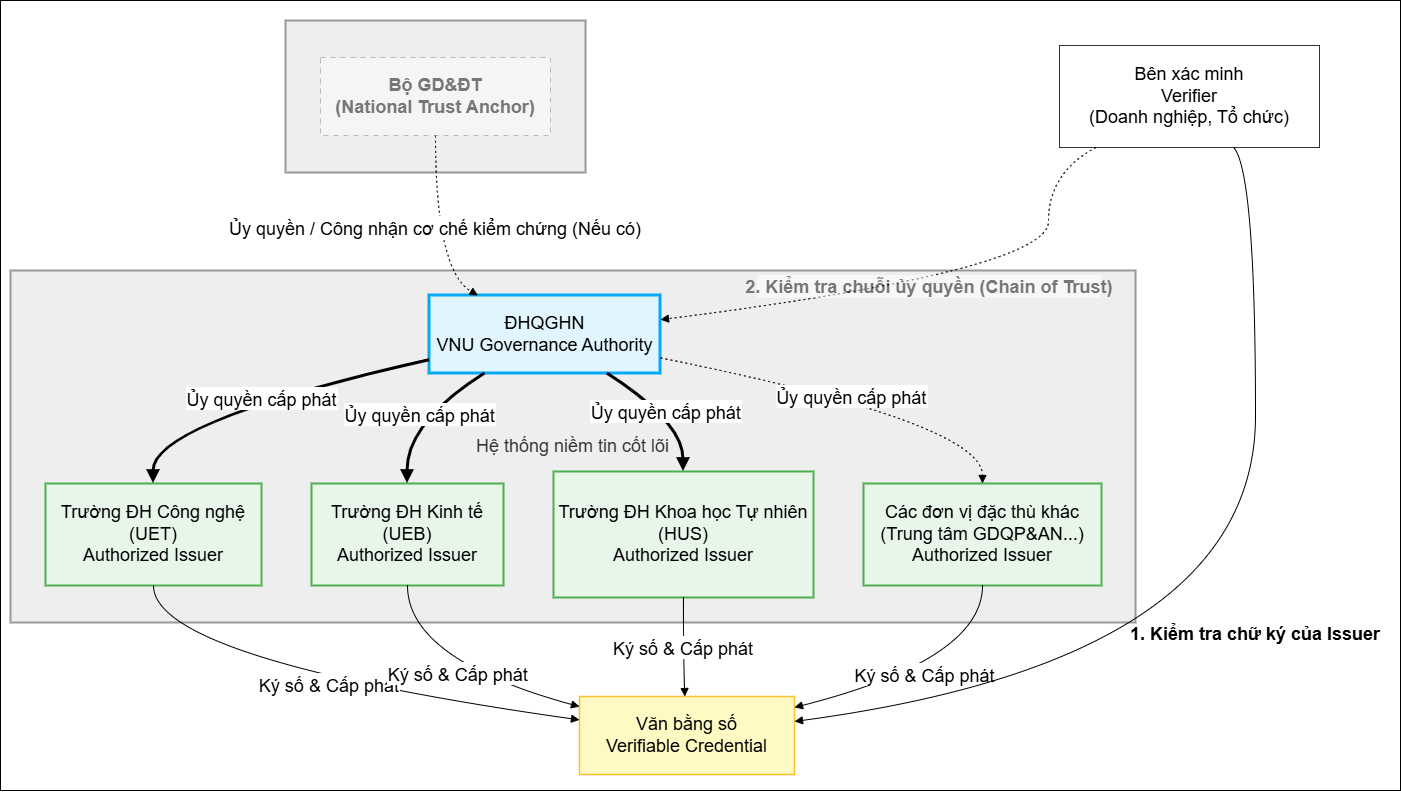
\includegraphics[width=0.88\textwidth]{images/trust-propagation-model.png}
    \caption{Mô hình lan truyền niềm tin theo cấu trúc phân cấp trong hệ thống văn bằng số}
    \label{fig:trust-propagation-model}
\end{figure}

\subsection{Sổ đăng ký tin cậy và yêu cầu đối với khung quản trị}

Thành phần hiện thực hóa tầng niềm tin thứ hai và thứ ba là \textbf{sổ đăng ký tin cậy} (trust registry) --- cơ chế lưu trữ và công bố trạng thái tin cậy của các bên phát hành trong hệ thống. Sổ đăng ký quản lý các thông tin: định danh của bên phát hành, trạng thái hiệu lực, phạm vi cấp phát được phép, thời hạn ủy quyền và quan hệ ủy quyền giữa các tổ chức. Theo nghĩa đó, nó là cầu nối giữa niềm tin kỹ thuật và niềm tin thể chế.

Khái niệm này đã được chuẩn hóa. Trust over IP Foundation công bố đặc tả Trust Registry Query Protocol phiên bản 2.0 vào tháng 4/2026 \cite{ToIP_TRQP2026}, định nghĩa một giao thức chỉ đọc để truy vấn dữ liệu có thẩm quyền từ các sổ đăng ký. Đặc tả xác định trường hợp sử dụng cốt lõi chính là câu hỏi đang xét: xác nhận rằng một bên phát hành được phép cấp một loại chứng thực cụ thể. Phiên bản 2.0 định nghĩa hai loại truy vấn --- truy vấn về thẩm quyền (authorization) và truy vấn về sự công nhận giữa các sổ đăng ký (recognition) --- và hoãn hai loại truy vấn khác, trong đó có truy vấn về ủy quyền nhiều cấp (delegation), sang phiên bản sau. Việc chính đặc tả chuẩn hóa còn hoãn phần ủy quyền nhiều cấp cho thấy đây là nội dung còn mở, và đó là một trong những điểm mà nghiên cứu này đóng góp.

Từ các phân tích trên, một khung quản trị niềm tin cần đáp ứng năm đặc tính:

\begin{itemize}
    \item \textbf{Tra cứu độc lập.} Trạng thái của bên phát hành phải tra cứu được mà không cần liên hệ bên phát hành hay cơ quan quản trị.
    \item \textbf{Lan truyền nhất quán.} Thay đổi về thẩm quyền phải có hiệu lực ngay trong các lần xác minh tiếp theo, không phụ thuộc vào việc bên xác minh có được thông báo hay không.
    \item \textbf{Phạm vi tường minh.} Thẩm quyền phải biểu diễn được theo phạm vi cụ thể, chứ không chỉ ở dạng nhị phân {``}được tin cậy / không được tin cậy{''}.
    \item \textbf{Dấu vết kiểm toán.} Mọi thay đổi quản trị phải để lại dấu vết không thể xóa, kể cả bởi chính cơ quan quản trị.
    \item \textbf{Phân tách khỏi lớp xác minh.} Thay đổi về quản trị không được đòi hỏi thay đổi ở phía bên xác minh.
\end{itemize}

Một đặc tính thứ sáu được các nghiên cứu gần đây nhấn mạnh và đáng được nêu, dù nằm ngoài phạm vi triển khai của khóa luận: trạng thái quản trị cần ở dạng \textbf{máy đọc được}, để ví và các tác nhân phần mềm tự động hóa được quyết định tin cậy thay vì đòi hỏi người dùng tự phán xét \cite{Weigl2025}. Yêu cầu này quan trọng vì nếu bên xác minh phải tự đọc và diễn giải một văn bản chính sách thì lớp quản trị không khác gì quy trình hành chính được số hóa. Trong thiết kế ở Chương 3, trạng thái thẩm quyền là dữ liệu có cấu trúc trên chuỗi nên thỏa mãn đặc tính này ở mức dữ liệu; phần chưa có là một biểu diễn máy đọc được cho \emph{chính sách} quản trị --- tức các quy tắc về điều kiện được cấp thẩm quyền, vốn hiện nằm ngoài hệ thống.

Năm đặc tính này trở thành tiêu chí thiết kế của khung quản trị được đề xuất ở Chương 3 và là căn cứ đối chiếu khi khảo sát các hệ thống hiện có.

\section{Khảo sát các hệ thống và giải pháp tiêu biểu}

Phần này phân tích các hệ thống tiêu biểu dưới lăng kính ba tầng niềm tin, nhằm xác định mỗi hệ thống giải quyết được tầng nào và để trống tầng nào.

\subsection{Blockcerts}

Blockcerts là một trong những hệ thống đầu tiên ứng dụng blockchain vào xác minh văn bằng, khởi nguồn từ MIT Media Lab \cite{Blockcerts2016}. Hệ thống biểu diễn chứng thực bằng JSON-LD, ký bằng khóa riêng của bên phát hành và neo giá trị băm của chứng thực lên một blockchain công khai.

Đóng góp lớn nhất của Blockcerts nằm ở tầng niềm tin kỹ thuật, và đóng góp đó mang tính lịch sử: hệ thống chứng minh được rằng xác minh độc lập hoàn toàn khả thi trong thực tế, ở quy mô thật, trước khi các chuẩn W3C đạt độ chín. Bên xác minh tự kiểm tra được chữ ký và tính toàn vẹn mà không cần liên hệ bên phát hành.

Tuy nhiên Blockcerts hầu như không giải quyết hai tầng còn lại. Hệ thống không có sổ đăng ký tin cậy hay cơ chế nào xác định tổ chức nào có thẩm quyền cấp phát; bất kỳ tổ chức nào cũng có thể sinh khóa và phát hành chứng thực {``}hợp lệ{''} về mặt kỹ thuật. Cơ chế thu hồi dựa vào danh sách do chính bên phát hành duy trì, nên bài toán quản trị ở quy mô hệ sinh thái vẫn còn nguyên. Đối chiếu với năm đặc tính ở Mục 2.6.3, Blockcerts đáp ứng đặc tính tra cứu độc lập đối với bản thân chứng thực nhưng không đáp ứng ba đặc tính liên quan tới thẩm quyền.

\noindent \textbf{Khoảng trống về thẩm quyền không phải một nhận xét lý thuyết}

Phần trên là một phân tích thiết kế, và một phân tích thiết kế có thể bị phản bác bằng lập luận rằng khoảng trống đó không gây hậu quả thực tế. Hai công trình phân tích an toàn cho thấy nó gây hậu quả thực tế, và cùng chỉ về một nguyên nhân gốc.

Baldi và cộng sự rà soát quy trình xác minh của Blockcerts và phát hiện một \textbf{tấn công mạo danh} \cite{Baldi2019}. Nguyên nhân nằm ở chỗ quy trình xác minh đối chiếu danh tính của bên phát hành với một \emph{hồ sơ bên phát hành không được xác thực}, lấy trực tuyến từ một địa chỉ do chính bên phát hành công bố. Kẻ tấn công vì vậy có thể dựng một hồ sơ bên phát hành giả cùng một chứng thực được sửa tương ứng, sao cho chứng thực giả \emph{không phân biệt được} với chứng thực thật bằng chính quy trình xác minh của hệ thống. Đáng chú ý là biện pháp khắc phục mà các tác giả đề xuất: tích hợp một hạ tầng khóa công khai cổ điển hoặc một hệ thống định danh phi tập trung --- nghĩa là bổ sung đúng lớp ràng buộc danh tính tổ chức mà hệ thống còn thiếu.

Bảy năm sau, cùng nhóm nghiên cứu báo cáo một \textbf{tấn công giả mạo} trên Block.co, một hệ thống chứng nhận văn bằng trên chuỗi đang được thương mại hóa, trong đó kẻ tấn công tạo được chứng thực giả mà hệ thống chấp nhận là hợp lệ \cite{Zonneveld2026}. Nguyên nhân gốc mà các tác giả xác định là việc \emph{thiếu một cơ quan có thẩm quyền được tin cậy}, khiến không thể ràng buộc danh tính pháp lý của một tổ chức với danh tính số của bên phát hành thuộc tổ chức đó; họ mô tả đây là một giới hạn nội tại của cách tiếp cận chứng nhận trên chuỗi và cảnh báo rằng các hệ thống tương tự có thể cũng dễ bị tấn công theo cách này.

Hai kết quả này có ý nghĩa trực tiếp đối với định hướng của khóa luận. Chúng cho thấy khoảng trống ở tầng niềm tin thể chế không phải một thiếu sót về sự hoàn chỉnh của mô hình mà là một \textbf{lớp lỗ hổng khai thác được}, và rằng việc bổ sung thêm cơ chế mật mã không lấp được nó --- cả hai hệ thống bị tấn công đều có chữ ký số hợp lệ và giá trị băm neo trên chuỗi đúng cách. Điều thiếu là một cơ chế để bên xác minh biết rằng \emph{khóa này thuộc về tổ chức có thẩm quyền đó}, và cơ chế đó thuộc phạm trù quản trị chứ không phải mật mã.

\subsection{Hạ tầng văn bằng số châu Âu: EDC và EBSI}

Liên minh Châu Âu phát triển hai thành phần bổ trợ nhau: European Digital Credentials for Learning cùng mô hình dữ liệu European Learning Model \cite{EDC_ELM} ở tầng chứng thực, và European Blockchain Services Infrastructure \cite{EBSI_TrustModel} ở tầng neo và quản trị.

Khác với Blockcerts, hệ thống này giải quyết đầy đủ cả ba tầng, và cách giải quyết tầng thứ ba đặc biệt đáng tham khảo. Mô hình niềm tin của EBSI xây dựng trên khái niệm \emph{tổ chức kiểm định được tin cậy}: các tổ chức này công nhận các bên phát hành cho một lĩnh vực và một phạm vi địa lý cụ thể, và bản thân sự công nhận đó cũng là một chứng thực có thể xác minh. Trong giáo dục, một bộ giáo dục quốc gia công nhận các trường đại học. Đồng thời, lược đồ của từng loại chứng thực được đăng ký trong một sổ đăng ký lược đồ riêng, nên bên xác minh kiểm tra được ba điều: định danh của bên phát hành, sự công nhận dành cho bên đó, và việc chứng thực có tuân theo lược đồ đã đăng ký.

Hai quan sát từ tài liệu kỹ thuật của EBSI có giá trị trực tiếp cho nghiên cứu này. Thứ nhất, sổ cái ghi nhận các quyết định về niềm tin nhưng không tạo ra chúng --- quyết định vẫn thuộc về cơ quan quản lý hoặc tổ chức kiểm định. Thứ hai, mỗi bên xác minh tự quyết định họ chấp nhận gốc niềm tin nào và theo chính sách nào. Hai nguyên tắc này được kế thừa trong thiết kế ở Chương 3.

Điểm mạnh khác của hệ thống châu Âu là sự gắn kết với hạ tầng pháp lý. Chứng thực không chỉ hợp lệ về mặt mật mã mà có giá trị pháp lý trong phạm vi Liên minh nhờ tích hợp với khung eIDAS \cite{eIDAS2014}, và khung này đã được sửa đổi năm 2024 để thiết lập Ví Định danh số Châu Âu \cite{eIDAS2_2024}, trong đó mỗi quốc gia thành viên có nghĩa vụ cung cấp ít nhất một ví vào cuối năm 2026.

Hạn chế của mô hình này là nó đánh đổi mức độ phi tập trung để lấy khả năng quản trị. Toàn bộ hệ sinh thái phụ thuộc mạnh vào hạ tầng và cơ chế quản trị của Liên minh, khiến nó khó áp dụng trực tiếp cho bối cảnh ngoài khối. Người học cũng có quyền kiểm soát hạn chế hơn, do dữ liệu chủ yếu nằm trên hạ tầng nền tảng thay vì trong ví cá nhân.

\subsection{Open Badges phiên bản 3.0}

Open Badges được thiết kế cho các chứng nhận vi mô và thành tích học tập linh hoạt. Phiên bản 3.0, được 1EdTech thông qua tháng 5/2024 \cite{OpenBadges2024}, đã tái cấu trúc để biểu diễn huy hiệu dưới dạng Verifiable Credential theo mô hình dữ liệu W3C, qua đó giải quyết tốt tầng niềm tin kỹ thuật.

Điểm mạnh của Open Badges là khả năng tổng hợp nhiều loại thành tích từ nhiều nguồn vào cùng một hồ sơ của người học, phù hợp với học tập mở và các chương trình đào tạo ngắn hạn. Tuy nhiên tầng niềm tin thể chế vẫn yếu: giá trị của một huy hiệu phụ thuộc chủ yếu vào uy tín xã hội của bên phát hành, và hệ thống không có sổ đăng ký tin cậy hay khung quản trị thống nhất để kiểm soát chất lượng bên phát hành. Đây là lựa chọn phù hợp với mục đích của chuẩn --- chứng nhận vi mô cần sự linh hoạt hơn là sự kiểm soát --- nhưng không đáp ứng yêu cầu của văn bằng đại học chính quy, nơi thẩm quyền cấp phát và sự công nhận pháp lý là điều kiện bắt buộc.

\subsection{Kiến trúc tham chiếu Trust over IP}

Trust over IP Foundation không phải một hệ thống triển khai mà là một kiến trúc tham chiếu cho hệ sinh thái định danh phi tập trung \cite{ToIP_Stack2022}. Đóng góp quan trọng nhất của kiến trúc này chính là nhận thức rằng niềm tin kỹ thuật không đủ để tạo niềm tin ở quy mô hệ sinh thái.

Phiên bản hiện hành của kiến trúc tổ chức tầng kỹ thuật thành bốn lớp: \emph{Trust Support} chứa các thành phần nền tảng như mô-đun tính toán tin cậy, lưu trữ an toàn và các sổ đăng ký dữ liệu có thể xác minh; \emph{Trust Spanning} thiết lập kết nối tin cậy giữa hai điểm cuối bằng một giao thức thống nhất, giữ vai trò tương tự lớp IP trong chồng giao thức TCP/IP; \emph{Trust Tasks} gồm các tác vụ nguyên tử như cấp phát và trình bày chứng thực; \emph{Trust Applications} là các ứng dụng gọi tới hai lớp dưới để thiết lập kết nối tin cậy.

Điểm đáng chú ý nhất về mặt phương pháp là cách kiến trúc xử lý vấn đề quản trị. Thay vì đặt quản trị thành một lớp riêng ở trên cùng, Trust over IP mô tả một \emph{chồng quản trị} song song với chồng kỹ thuật, trong đó siêu mô hình quản trị áp dụng được ở cả bốn lớp \cite{ToIP_GovMetamodel2022}. Cách nhìn này chính xác hơn: quản trị không phải một tầng chức năng mà là một chiều xuyên suốt của hệ thống. Thiết kế ở Chương 3 kế thừa quan điểm này ở mức nguyên tắc, dù vẫn trình bày quản trị thành một lớp riêng để giữ sự rõ ràng trong mô tả.

Hạn chế của Trust over IP là nó dừng ở mức kiến trúc tham chiếu. Nó không áp đặt blockchain, phương thức DID hay lược đồ cụ thể, và không cung cấp một mô hình triển khai cho lĩnh vực giáo dục; mỗi hệ sinh thái vẫn phải tự xây dựng khung quản trị phù hợp với bối cảnh của mình.

\subsection{EduCTX và các công trình học thuật liên quan}

EduCTX của Turkanović và cộng sự \cite{Turkanovic2018} là một trong những đề xuất học thuật có ảnh hưởng về nền tảng tín chỉ liên trường trên blockchain. Công trình xác định rõ bài toán liên thông định danh trong môi trường giáo dục đa cơ sở --- vấn đề thứ hai trong ba vấn đề của nghiên cứu này --- và đề xuất mô hình biểu diễn tín chỉ học tập dưới dạng token. Hạn chế là mô hình tập trung vào việc biểu diễn và chuyển đổi tín chỉ hơn là vào bài toán thẩm quyền cấp phát.

Các khảo sát hệ thống gần đây cho thấy khoảng trống về quản trị là đặc điểm chung của cả lĩnh vực. Rà soát 63 bài báo giai đoạn 2018--2023 về quản trị trong kiểm định giáo dục trên nền blockchain, De Alwis và cộng sự kết luận rằng tài liệu hiện có hầu như không có đề xuất nào về một khung quản trị, trong khi ở mô hình truyền thống chính khung quản trị mới là yếu tố bảo đảm tính xác thực của văn bằng \cite{DeAlwis2025}. Báo cáo chính sách của Trung tâm Nghiên cứu Chung thuộc Ủy ban Châu Âu về blockchain trong giáo dục cũng nêu bật rằng các rào cản chính không nằm ở công nghệ mà ở quản trị và tiêu chuẩn hóa \cite{Grech2017}. Ở phía định danh, các khảo sát của Mühle và cộng sự \cite{Muhle2018} cùng Schardong và Custódio \cite{Schardong2022} xác nhận rằng cơ chế thiết lập niềm tin ở mức hệ sinh thái là một trong những thành phần ít được giải quyết nhất của các hệ thống định danh tự chủ.

\subsection{Bối cảnh Việt Nam}

Tại Việt Nam, hạ tầng liên quan đang hình thành nhanh. Nền tảng blockchain quốc gia NDAChain, ra mắt năm 2025, được thiết kế như một lớp hạ tầng trung gian để xác thực và ghi nhận giao dịch dữ liệu, theo mô hình được cấp phép với tập nút xác thực được lựa chọn và giám sát; nền tảng đi kèm một giải pháp định danh phi tập trung và một ứng dụng quản lý định danh \cite{NDAChain2025}. Khung kiến trúc tổng thể quốc gia số công bố tháng 10/2025 xác định blockchain quốc gia là hạ tầng số dùng chung. Song song, hệ thống định danh điện tử công dân đã đạt độ phủ rộng và theo Thông tư 10/2026/TT-BGDĐT \cite{TT10_2026}, việc tra cứu văn bằng trên nền tảng này có thể thay thế bản sao từ sổ gốc.

Đặc điểm của bối cảnh này là các khối hạ tầng đã có nhưng lớp quản trị thẩm quyền cấp phát trong lĩnh vực giáo dục thì chưa được định hình. Đây là lý do nghiên cứu thiết kế khung quản trị độc lập với nền tảng neo cụ thể: mô hình thẩm quyền có thể chuyển sang một hạ tầng khác mà không cần thiết kế lại, miễn hạ tầng đó cung cấp ba tính chất đã nêu ở Mục 2.5.1.

\subsection{Tổng hợp khảo sát}

\begin{longtable}{|p{2.4cm}|p{2.5cm}|p{3.1cm}|p{3.1cm}|p{2.6cm}|}
\caption{Tổng hợp khảo sát các hệ thống tiêu biểu theo ba tầng niềm tin}
\label{tab:trust-layer-survey} \\

\hline
\textbf{Hệ thống} &
\textbf{Niềm tin kỹ thuật} &
\textbf{Niềm tin thể chế} &
\textbf{Niềm tin quản trị} &
\textbf{Holder giữ dữ liệu} \\
\hline
\endfirsthead

\hline
\textbf{Hệ thống} &
\textbf{Niềm tin kỹ thuật} &
\textbf{Niềm tin thể chế} &
\textbf{Niềm tin quản trị} &
\textbf{Holder giữ dữ liệu} \\
\hline
\endhead

\hline
\endfoot

\hline
\endlastfoot

Blockcerts
& Đầy đủ: chữ ký và băm neo trên chuỗi
& Không có. Khoảng trống này đã bị khai thác: tấn công mạo danh qua hồ sơ bên phát hành không được xác thực \cite{Baldi2019}
& Không có: thu hồi dựa trên danh sách do bên phát hành tự giữ
& Có
\\ \hline

EDC / EBSI
& Đầy đủ
& Đầy đủ: tổ chức kiểm định công nhận bên phát hành theo lĩnh vực và địa bàn
& Đầy đủ nhưng tập trung: phụ thuộc hạ tầng và quản trị của Liên minh
& Hạn chế: dữ liệu chủ yếu trên hạ tầng nền tảng
\\ \hline

Open Badges 3.0
& Đầy đủ sau khi tích hợp mô hình dữ liệu W3C
& Yếu: giá trị phụ thuộc uy tín xã hội của bên phát hành
& Không có sổ đăng ký hay khung quản trị thống nhất
& Có
\\ \hline

Trust over IP
& Mô tả ở mức kiến trúc tham chiếu
& Mô tả: chồng quản trị song song chồng kỹ thuật
& Mô tả đầy đủ nhất về khái niệm, không có triển khai cho giáo dục
& Theo thiết kế
\\ \hline

EduCTX
& Đầy đủ cho biểu diễn tín chỉ
& Không phải trọng tâm của công trình
& Không đề cập cơ chế thu hồi thẩm quyền
& Có
\\ \hline

Mô hình đề xuất
& Đầy đủ, kèm bước đối chiếu nội dung với băm đã neo
& Chuỗi thẩm quyền đặc tả thành mã thi hành, có phạm vi và thời hạn
& Trạng thái quản trị công khai trên chuỗi, dấu vết không thể xóa
& Có: ví không lưu ký
\\ \hline

\end{longtable}


\section{Khoảng trống nghiên cứu}

\subsection{Phân loại khoảng trống theo tầng}

Khảo sát ở Mục 2.7 cho phép xác định khoảng trống cụ thể hơn so với phát biểu chung {``}thiếu quản trị niềm tin{''}. Tuy nhiên, nếu chỉ liệt kê các khoảng trống ở dạng danh sách ngang hàng thì không đánh giá được chúng thuộc loại nào và một nghiên cứu đơn lẻ có thể xử lý tới đâu --- một khoảng trống ở tầng chuẩn hóa đòi hỏi quá trình đồng thuận của cả cộng đồng, trong khi một khoảng trống ở tầng kiến trúc có thể xử lý trong phạm vi một hệ thống.

Vì vậy phần này phân loại khoảng trống thành sáu tầng, mỗi tầng kèm bằng chứng từ tài liệu và phạm vi xử lý của nghiên cứu này. Bảng \ref{tab:gap-taxonomy} tổng hợp, và các mục dưới đây phân tích từng tầng.

\begin{longtable}{|c|p{2.9cm}|p{4.4cm}|p{2.5cm}|p{2.6cm}|}
\caption{Phân loại khoảng trống nghiên cứu theo tầng và phạm vi can thiệp của khóa luận}
\label{tab:gap-taxonomy} \\

\hline
\textbf{Mã} & \textbf{Tầng} & \textbf{Nội dung khoảng trống} & \textbf{Bằng chứng} & \textbf{Khóa luận xử lý} \\
\hline
\endfirsthead

\hline
\textbf{Mã} & \textbf{Tầng} & \textbf{Nội dung khoảng trống} & \textbf{Bằng chứng} & \textbf{Khóa luận xử lý} \\
\hline
\endhead

\hline
\endfoot

\hline
\endlastfoot

G1 & Chuẩn hóa
& Chuẩn về truy vấn sổ đăng ký tin cậy còn hoãn phần ủy quyền nhiều cấp; chuẩn về trạng thái chứng thực không biểu diễn thẩm quyền
& \cite{ToIP_TRQP2026}, \cite{W3C_BitstringStatusList2025}
& \textbf{Góp một điểm dữ liệu}: đưa ra cách biểu diễn cụ thể và chứng minh nó chạy được
\\ \hline

G2 & Kiến trúc
& Lớp quản trị khi tồn tại thường là cơ sở dữ liệu do một tổ chức vận hành, nên chỉ \emph{di chuyển} sự phụ thuộc vào trung gian chứ không loại bỏ
& \cite{Baldi2019}, \cite{Zonneveld2026}, \cite{SSI_Survey2025}
& \textbf{Xử lý trực tiếp}: sổ đăng ký là trạng thái hợp đồng trên chuỗi công khai
\\ \hline

G3 & Biểu diễn thẩm quyền
& Thẩm quyền biểu diễn ở dạng nhị phân; thiếu ba chiều phạm vi, thời hạn và số cấp ủy quyền
& \cite{Blockcerts2016}, \cite{OpenBadges2024}, \cite{ToIP_TRQP2026}
& \textbf{Xử lý trực tiếp}: mặt nạ bit, trường thời hạn, ủy quyền hai cấp có ràng buộc
\\ \hline

G4 & Ngữ nghĩa xác minh
& Quy trình xác minh không phân biệt loại thất bại; nhiều hệ thống không đối chiếu nội dung với giá trị băm đã neo
& Mục 2.7.1, Mục 2.7.3
& \textbf{Xử lý trực tiếp}: bảy bước có báo cáo riêng, gồm bước đối chiếu nội dung
\\ \hline

G5 & Phương pháp đánh giá
& Lĩnh vực thiếu nghiên cứu người dùng: chỉ 2 trong 47 công trình được phân tích có đánh giá tính khả dụng; các khung niềm tin chỉ kiểm chứng bằng cài đặt hợp đồng
& \cite{Ambati2026}, \cite{DeSalve2023}
& \textbf{Không xử lý} --- khóa luận nằm trong cùng giới hạn này; thừa nhận tại Mục 4.11 và Mục 5.3
\\ \hline

G6 & Bối cảnh
& Tại Việt Nam, hành lang pháp lý và hạ tầng số đã hình thành nhưng chưa có lớp quản trị thẩm quyền cấp phát cho lĩnh vực giáo dục
& \cite{TT10_2026}, \cite{LuatBVDLCN2025}, \cite{NDAChain2025}
& \textbf{Xử lý một phần}: trong phạm vi một trường hợp nghiên cứu
\\ \hline

\end{longtable}


\noindent \textbf{G1 --- Khoảng trống ở tầng chuẩn hóa}

Các đặc tả hiện hành chưa bao phủ đầy đủ việc biểu diễn thẩm quyền. Đặc tả Trust Registry Query Protocol phiên bản 2.0 định nghĩa hai loại truy vấn --- về thẩm quyền và về sự công nhận lẫn nhau giữa các sổ đăng ký --- nhưng \textbf{hoãn loại truy vấn về ủy quyền nhiều cấp sang phiên bản sau} \cite{ToIP_TRQP2026}. Ở phía trạng thái chứng thực, cơ chế danh sách bit của W3C \cite{W3C_BitstringStatusList2025} giải quyết rất tốt bài toán trạng thái nhưng không biểu diễn thẩm quyền của bên phát hành; hai bài toán này được chuẩn hóa độc lập và chưa có cơ chế gắn kết chúng.

Đây là khoảng trống mà một khóa luận \emph{không thể lấp}, vì việc chuẩn hóa thuộc về quá trình đồng thuận của cộng đồng. Điều nghiên cứu này có thể làm là đưa ra một cách biểu diễn cụ thể cho phần còn hoãn và chứng minh nó chạy được, qua đó đóng góp một điểm dữ liệu cho quá trình chuẩn hóa.

\noindent \textbf{G2 --- Khoảng trống ở tầng kiến trúc}

Khi lớp quản trị tồn tại, nó thường được hiện thực hóa bằng một cơ sở dữ liệu do một tổ chức vận hành. Hạ tầng văn bằng số châu Âu là ví dụ hoàn chỉnh nhất của hướng này \cite{EBSI_TrustModel}, và nó hoạt động tốt trong phạm vi có một cơ quan quản trị được công nhận.

Quan sát quan trọng là: cách làm đó \textbf{di chuyển} sự phụ thuộc vào trung gian chứ không loại bỏ nó. Bên xác minh không còn phải tin cơ sở cấp phát, nhưng phải tin tổ chức vận hành sổ đăng ký. Khảo sát tổng quan về định danh tự chủ ghi nhận rủi ro tập trung hóa bên phát hành như một nguy cơ quản trị có thể tạo ra điểm hỏng đơn lẻ \cite{SSI_Survey2025}. Đây là khoảng trống mà nghiên cứu này xử lý trực tiếp: đặt sổ đăng ký thành trạng thái của một hợp đồng trên chuỗi công khai.

Cần ghi nhận rằng hướng này đã có công trình đi trước. Eer, Diaz và Kohlweiss đề xuất một sổ đăng ký tin cậy theo hướng từ dưới lên, dựa trên uy tín và kèm cơ chế khuyến khích tham gia trung thực \cite{Eer2022}; De Salve và cộng sự đề xuất một khung niềm tin nhiều lớp dựa trên quan hệ tin cậy giữa các tác nhân, cài đặt bằng hợp đồng thông minh \cite{DeSalve2023}. Hai công trình này giải quyết câu hỏi {``}bên xác minh nên tin ai{''} theo hướng \emph{uy tín phân tán}; nghiên cứu này giải quyết theo hướng \emph{ủy quyền thể chế có cấu trúc}. Hai hướng bổ trợ nhau và phù hợp với hai loại hệ sinh thái khác nhau: hướng uy tín phù hợp khi không có cơ quan quản trị được công nhận, hướng ủy quyền phù hợp khi có --- và trong giáo dục đại học thì luôn có.

\noindent \textbf{G3 --- Khoảng trống ở tầng biểu diễn thẩm quyền}

Phần lớn hệ thống biểu diễn thẩm quyền ở dạng nhị phân: một bên phát hành được tin cậy hoặc không. Ba chiều thông tin bị thiếu, và cả ba đều có trong thực tiễn quản trị giáo dục:

\begin{itemize}
    \item \textbf{Phạm vi.} Một trường được kiểm định cho một số ngành và trình độ nhất định, không phải cho mọi loại văn bằng.
    \item \textbf{Thời hạn.} Thẩm quyền gắn với một chu kỳ kiểm định và tự hết hiệu lực nếu không được gia hạn.
    \item \textbf{Số cấp.} Một trường được ủy quyền có thể cần ủy quyền tiếp cho một đơn vị trực thuộc.
\end{itemize}

Hạ tầng châu Âu xử lý được hai chiều đầu thông qua khái niệm tổ chức kiểm định công nhận bên phát hành theo lĩnh vực và địa bàn \cite{EBSI_TrustModel}. Chiều thứ ba thì, như đã nêu ở G1, còn hoãn ngay ở tầng chuẩn hóa. Đây là khoảng trống mà nghiên cứu này xử lý đầy đủ nhất.

\noindent \textbf{G4 --- Khoảng trống ở tầng ngữ nghĩa của quy trình xác minh}

Khi một chứng thực bị từ chối, bên xác minh cần biết nguyên nhân là nội dung bị sửa, hay chứng thực đã bị thu hồi, hay bên phát hành đã mất thẩm quyền --- ba tình huống đòi hỏi ba cách xử lý hoàn toàn khác nhau. Một kết quả {``}không hợp lệ{''} chung không đủ để hành động.

Liên quan tới đây là một khoảng trống cụ thể hơn: nhiều hệ thống kiểm trạng thái chứng thực nhưng không đối chiếu \emph{nội dung} với giá trị băm đã neo, nên không phát hiện được trường hợp nội dung bị sửa sau khi cấp. Mục 3.6.1 và Mục 4.8.3 phân tích và kiểm chứng điểm này.

\noindent \textbf{G5 --- Khoảng trống ở tầng phương pháp đánh giá}

Đây là khoảng trống mà nghiên cứu này \emph{cũng mắc phải}, nên cần nêu trung thực. Khảo sát hệ thống của Ambati và cộng sự trên 80 nguồn, trong đó phân tích 47 công trình khoa học và 12 hệ thống đang vận hành, ghi nhận rằng chỉ \textbf{2 trong 47} công trình có nghiên cứu người dùng hoặc đánh giá tính khả dụng, và gọi đây là một khoảng trống nghiêm trọng của lĩnh vực \cite{Ambati2026}. Các khung niềm tin được đề xuất thường được kiểm chứng bằng cách cài đặt hợp đồng thông minh và đo hiệu năng \cite{DeSalve2023}, chứ không bằng nghiên cứu người dùng hay triển khai thực địa.

Trong số rất ít nghiên cứu người dùng đã có, nghiên cứu của Zaeem và cộng sự ghi nhận rằng quá trình khởi tạo gây khó hiểu và người dùng lo lắng về việc mất khóa riêng \cite{Zaeem2021} --- đúng hai vấn đề mà mô hình ví không lưu ký ở Mục 2.3.4 đặt ra. Nghiên cứu này ở trong đúng nhóm thiếu bằng chứng đó: nó kiểm chứng bằng bộ kiểm thử và phép đo hiệu năng, không có nghiên cứu người dùng. Việc đặt khoảng trống này thành một tầng riêng có hai mục đích: thừa nhận giới hạn của kết quả thu được (Mục 4.11), và xác định rõ rằng kết luận của khóa luận là về \emph{tính khả thi kỹ thuật}, không phải về \emph{mức độ tiếp nhận}. Nghiên cứu phỏng vấn về yếu tố quyết định mức độ tiếp nhận định danh tự chủ cho thấy hai câu hỏi này tách biệt và không suy ra được từ nhau \cite{SSI_Adoption2025}.

\noindent \textbf{G6 --- Khoảng trống ở tầng bối cảnh}

Khoảng trống này mang tính địa phương nhưng là lý do trực tiếp của đề tài. Tại Việt Nam, ba điều kiện đã hội đủ: hành lang pháp lý công nhận giá trị pháp lý của văn bằng số \cite{TT10_2026}, quy định về bảo vệ dữ liệu cá nhân đặt ra ràng buộc kiến trúc rõ ràng \cite{LuatBVDLCN2025}, và hạ tầng số quốc gia gồm nền tảng blockchain và giải pháp định danh phi tập trung đang được triển khai \cite{NDAChain2025}.

Điều còn thiếu là lớp quản trị thẩm quyền cấp phát trong lĩnh vực giáo dục: chưa có cơ chế nào cho phép một bên thứ ba kiểm chứng rằng một đơn vị được phép cấp một loại văn bằng cụ thể. Các hạ tầng nêu trên cung cấp nền neo và nền định danh, nhưng không tự sinh ra lớp quản trị đó --- nó phải được thiết kế riêng cho từng lĩnh vực, giống như hạ tầng châu Âu phải thiết kế riêng mô hình tổ chức kiểm định cho giáo dục.

\subsection{Định hướng của nghiên cứu}

Từ phân loại trên, phạm vi can thiệp của khóa luận được xác định như sau. Nghiên cứu xử lý \textbf{trực tiếp} ba tầng G2, G3 và G4, là ba tầng thuộc phạm vi kiến trúc và có thể kiểm chứng trong một hệ thống đơn lẻ. Nghiên cứu \textbf{đóng góp một điểm dữ liệu} cho G1 bằng cách đưa ra một cách biểu diễn cụ thể cho phần mà chuẩn còn hoãn và chứng minh nó chạy được. Nghiên cứu \textbf{xử lý một phần} G6 trong phạm vi một trường hợp nghiên cứu. Và nghiên cứu \textbf{không xử lý} G5 --- nó nằm trong cùng giới hạn phương pháp mà G5 mô tả, và điều này được thừa nhận thay vì bỏ qua.

Hướng tiếp cận tương ứng: dùng các chuẩn mở về định danh phi tập trung và chứng thực có thể xác minh làm nền kỹ thuật, bảo đảm xác minh độc lập và quyền kiểm soát dữ liệu của người học; đồng thời xây dựng một khung quản trị niềm tin trong đó chuỗi thẩm quyền được đặc tả thành mã thi hành trên một hạ tầng công khai bất biến, với phạm vi và thời hạn tường minh, và quy trình xác minh phân biệt rõ các loại thất bại. Kiến trúc hiện thực hóa hướng tiếp cận này được trình bày ở Chương 3.

% Chương 3: Đề xuất kiến trúc và khung quản trị niềm tin
\chapter{ĐỀ XUẤT KIẾN TRÚC VÀ KHUNG QUẢN TRỊ NIỀM TIN}

Chương này trình bày đóng góp lý thuyết trung tâm của nghiên cứu. Nội dung đi từ yêu cầu (Mục 3.1) qua nguyên tắc thiết kế (Mục 3.2) đến kiến trúc tổng thể (Mục 3.3), sau đó tập trung vào khung quản trị niềm tin (Mục 3.4) --- phần lấp đầy khoảng trống đã xác định ở Mục 2.8. Mục 3.5 đặc tả mô hình dữ liệu, Mục 3.6 đặc tả quy trình xác minh. Mục 3.7 phân tích mô hình đe dọa, qua đó kiểm tra lại tính đầy đủ của thiết kế. Hai mục cuối trình bày các đánh đổi và đối chiếu với các kiến trúc tham chiếu.

\section{Yêu cầu hệ thống}

\subsection{Mục tiêu thiết kế}

Hệ thống được thiết kế để giải quyết đồng thời hai bài toán mà Chương 2 đã chỉ ra là thuộc hai tầng khác nhau: xác minh kỹ thuật và quản trị thẩm quyền. Điều đó dẫn tới năm mục tiêu thiết kế, trong đó mục tiêu cuối là điểm phân biệt với các hệ thống định danh tự chủ thông thường.

Thứ nhất, hệ thống cung cấp một hạ tầng định danh phi tập trung cho mọi thực thể tham gia --- người học, cơ sở đào tạo, bên xác minh và cơ quan quản trị. Mỗi thực thể sở hữu một định danh độc lập với hệ thống thông tin của bất kỳ tổ chức nào, kiểm soát bằng khóa mật mã mà chủ thể giữ.

Thứ hai, hệ thống hỗ trợ toàn bộ vòng đời của chứng thực: cấp phát, lưu trữ trong ví của chủ thể, trình bày, xác minh và thu hồi. Việc xác minh phải thực hiện được mà không cần tương tác với đơn vị cấp phát.

Thứ ba, hệ thống bảo đảm khả năng liên thông giữa nhiều cơ sở: người học dùng cùng một định danh để tiếp nhận và quản lý chứng thực từ nhiều đơn vị trong hệ sinh thái, và trình bày chúng trong một lần xác minh duy nhất.

Thứ tư, hệ thống tuân theo nguyên tắc bảo vệ quyền riêng tư từ gốc \cite{Cavoukian2009}: dữ liệu cá nhân không được ghi lên hạ tầng công khai bất biến, chủ thể kiểm soát việc chia sẻ, và mọi thao tác quản trị đều để lại dấu vết kiểm chứng được.

Thứ năm, và quan trọng nhất đối với đóng góp của nghiên cứu, hệ thống xây dựng một khung quản trị niềm tin cho môi trường giáo dục liên trường, trong đó thẩm quyền cấp phát được thiết lập, giới hạn phạm vi, giới hạn thời hạn, ủy quyền lại và thu hồi theo cách mà bất kỳ bên thứ ba nào cũng kiểm chứng được công khai --- thay vì dựa vào uy tín hoặc vào một quy trình thủ công.

\subsection{Yêu cầu chức năng}

Các yêu cầu chức năng được xây dựng xoay quanh vòng đời chứng thực, đồng thời bổ sung nhóm yêu cầu về quản trị thẩm quyền mà mô hình ba bên thuần túy không bao gồm. Mỗi yêu cầu đi kèm một tiêu chí kiểm chứng có thể quan sát được; đây là điều kiện đã đặt ra ở Mục 1.5.1 khi chọn khung phương pháp khoa học thiết kế.

\begin{longtable}{|c|p{2.6cm}|p{4.4cm}|p{4.8cm}|p{1.3cm}|}
\caption{Danh sách yêu cầu chức năng\label{tab:functional-requirements}} \\
\hline
\textbf{Mã} & \textbf{Yêu cầu} & \textbf{Mô tả} & \textbf{Tiêu chí kiểm chứng} & \textbf{Kịch bản} \\
\hline
\endfirsthead

\hline
\textbf{Mã} & \textbf{Yêu cầu} & \textbf{Mô tả} & \textbf{Tiêu chí kiểm chứng} & \textbf{Kịch bản} \\
\hline
\endhead

\hline
\endfoot

\hline
\endlastfoot

F1 & Đăng ký định danh
& Mọi thực thể sinh khóa phía máy khách, dựng DID Document và đăng ký định danh kèm giá trị băm lên chuỗi
& Phân giải định danh thành công; giá trị băm tính lại khớp giá trị đã neo trên chuỗi
& KB1 \\ \hline

F2 & Xoay vòng khóa và giữ lịch sử phiên bản
& Chủ sở hữu cập nhật DID Document bằng chữ ký của khóa hiện tại; các phiên bản trước vẫn truy xuất được
& Cập nhật tăng số phiên bản; chứng thực cấp bằng khóa cũ vẫn xác minh được
& KB1 \\ \hline

F3 & Quản lý vòng đời thẩm quyền
& Cơ quan quản trị phê duyệt bên phát hành kèm phạm vi và thời hạn, cập nhật phạm vi, đình chỉ và thu hồi
& Phê duyệt thành công; thu hồi có hiệu lực ngay trong lần xác minh tiếp theo; mọi thao tác có mã giao dịch trên chuỗi
& KB2, KB5 \\ \hline

F4 & Ủy quyền nhiều cấp có ràng buộc
& Bên phát hành có bit ủy quyền phê duyệt được bên phát hành cấp dưới trong phạm vi hẹp hơn
& Phạm vi vượt tập cha bị từ chối; thời hạn vượt thời hạn cha bị từ chối; bit ủy quyền không truyền tiếp
& KB2 \\ \hline

F5 & Chuyển quyền gốc hai bước
& Quản trị viên gốc đề cử; người được đề cử tự ký để tiếp nhận; đề cử có thể bị hủy trước khi tiếp nhận
& Quyền chỉ chuyển sau khi người được đề cử ký; địa chỉ không được đề cử ký nhận sẽ thất bại
& KB2 \\ \hline

F6 & Cấp phát chứng thực
& Bên phát hành dựng chứng thực theo mô hình dữ liệu W3C, ký bằng khóa riêng và ghi bản ghi neo lên chuỗi
& Chứng thực hợp lệ về cấu trúc; chữ ký Ed25519 kiểm tra được; loại văn bằng ngoài phạm vi bị từ chối tại hợp đồng
& KB3 \\ \hline

F7 & Lưu trữ an toàn phía chủ thể
& Khóa riêng được mã hóa và chỉ lưu dạng bản mã trên thiết bị của chủ thể
& Bản mã AES-256-GCM \cite{NIST_SP800_38D}; không gói tin nào gửi lên dịch vụ chứa khóa riêng hoặc mật khẩu
& KB1 \\ \hline

F8 & Trình bày có chọn lọc
& Chủ thể dựng bản trình bày từ tập chứng thực mình chọn và ký bằng khóa riêng
& Bản trình bày chỉ chứa các chứng thực được chọn; chữ ký của chủ thể kiểm tra được
& KB4 \\ \hline

F9 & Xác minh tính toàn vẹn và quyền sở hữu
& Bên xác minh kiểm tra chữ ký của bên phát hành, chữ ký của chủ thể, và đối chiếu nội dung với giá trị băm đã neo
& Phát hiện được nội dung bị sửa sau khi cấp; phát hiện được bản trình bày do thực thể khác ký
& KB4, KB7 \\ \hline

F10 & Xác minh thẩm quyền độc lập
& Bên xác minh tra cứu trạng thái thẩm quyền của bên phát hành trực tiếp từ chuỗi
& Xác minh hoàn tất khi dịch vụ của bên phát hành không hoạt động; phát hiện bên phát hành đã bị thu hồi hoặc hết hạn ủy quyền
& KB4, KB5 \\ \hline

F11 & Quản lý trạng thái chứng thực
& Thu hồi, đình chỉ và kích hoạt lại chứng thực; trạng thái phản ánh ngay trong mọi lần xác minh sau đó
& Chứng thực bị thu hồi bị từ chối; chứng thực hợp lệ vẫn đạt; đơn vị hết hạn ủy quyền vẫn thu hồi được chứng thực mình đã cấp
& KB6, KB7 \\ \hline

F12 & Dấu vết kiểm toán
& Mọi thao tác thay đổi trạng thái đều được ghi nhận kèm chủ thể thực hiện, đối tượng và thời điểm
& Nhật ký trả về đúng các thao tác đã thực hiện với cùng bộ tên hành động ở mọi cài đặt của tầng dịch vụ
& KB2, KB6 \\ \hline

\end{longtable}


\subsection{Yêu cầu phi chức năng}

\begin{longtable}{|c|p{2.6cm}|p{4.6cm}|p{5.4cm}|}
\caption{Danh sách yêu cầu phi chức năng}
\label{tab:non-functional-requirements} \\

\hline
\textbf{Mã} & \textbf{Nhóm} & \textbf{Yêu cầu} & \textbf{Tiêu chí đo lường} \\
\hline
\endfirsthead

\hline
\textbf{Mã} & \textbf{Nhóm} & \textbf{Yêu cầu} & \textbf{Tiêu chí đo lường} \\
\hline
\endhead

\hline
\endfoot

\hline
\endlastfoot

N1 & Niềm tin &
Thẩm quyền của bên phát hành kiểm chứng được độc lập &
Tra cứu trạng thái thẩm quyền không cần liên hệ bên phát hành hay cơ quan quản trị, không cần tài khoản hay thỏa thuận trước \\ \hline

N2 & Niềm tin &
Mọi thay đổi quản trị để lại dấu vết bất biến &
Toàn bộ thao tác ghi sổ đăng ký tin cậy đều có mã giao dịch trên chuỗi; không có thao tác nào xóa hoặc sửa được lịch sử, kể cả từ quản trị viên gốc \\ \hline

N3 & Niềm tin &
Quy tắc phân quyền được thi hành ở nơi không thể bỏ qua &
Mọi quy tắc phân quyền nằm trong hợp đồng; gọi trực tiếp hợp đồng mà bỏ qua tầng dịch vụ vẫn bị chặn \\ \hline

N4 & An toàn &
Không có thông tin học thuật đọc trực tiếp được từ dữ liệu trên chuỗi &
Liệt kê đầy đủ các trường được ghi vào hợp đồng; không trường nào chứa nội dung văn bằng ở dạng đọc được. Lưu ý: tiêu chí này \textbf{không} đồng nghĩa với {``}không có dữ liệu cá nhân trên chuỗi{''} --- xem phân tích tại Mục 2.5.4 và Mục 3.5.1 \\ \hline

N5 & An toàn &
Khóa riêng không rời khỏi thiết bị của chủ thể &
Kiểm tra toàn bộ gói tin gửi lên dịch vụ, không gói tin nào chứa khóa riêng, mật khẩu hay cụm từ khôi phục \\ \hline

N6 & An toàn &
Phát hiện toàn bộ kịch bản gian lận được định nghĩa trước &
Mỗi kịch bản ở Mục 3.7.2 bị chặn, và thông điệp từ chối khớp đúng nguyên nhân thật chứ không do một phép kiểm khác chặn trước \\ \hline

N7 & Quyền riêng tư &
Chủ thể kiểm soát việc chia sẻ &
Bản trình bày chỉ chứa các chứng thực chủ thể chọn; không thành phần nào của hệ thống trình bày được chứng thực thay chủ thể \\ \hline

N8 & Phi tập trung &
Xác minh không phụ thuộc bên phát hành trực tuyến &
Xác minh hoàn tất khi dịch vụ của bên phát hành ngừng hoạt động, chỉ cần chuỗi và lớp lưu trữ ngoài chuỗi \\ \hline

N9 & Liên thông &
Tuân thủ chuẩn W3C DID Core và mô hình dữ liệu chứng thực &
Cấu trúc DID Document và chứng thực hợp lệ theo đặc tả \cite{W3C_DIDCore2022, W3C_VCDM2025}; các điểm chưa tuân thủ được liệt kê tường minh \\ \hline

N10 & Liên thông &
Tầng dịch vụ có hợp đồng giao diện ổn định, không phụ thuộc cài đặt &
Hai cài đặt độc lập trả cùng kết quả và cùng mã trạng thái cho cùng một yêu cầu, kể cả với dữ liệu vào không hợp lệ \\ \hline

N11 & Hiệu năng &
Thời gian xác minh ở mức chấp nhận được &
Phân vị 95 của các tuyến đọc không vượt 500\,ms dưới tải đồng thời. \textbf{Yêu cầu này không kiểm chứng được} trên cách thiết lập đo hiện tại --- xem phân tích tại Mục 4.9.6 \\ \hline

N12 & Hiệu năng &
Hệ thống không sinh lỗi chức năng dưới tải &
Không yêu cầu nào thất bại và không yêu cầu nào chạm hạn mức trong toàn bộ phép đo. Đây là một phép đếm nên không bị ảnh hưởng bởi nhiễu đo \\ \hline

N13 & Khả năng mở rộng &
Kiến trúc hỗ trợ mở rộng ngang &
Tầng dịch vụ không giữ trạng thái phiên; mọi trạng thái dùng chung nằm trong cơ sở dữ liệu dùng chung hoặc trên chuỗi \\ \hline

\end{longtable}


Một lưu ý về cách đặt yêu cầu phi chức năng. Các tiêu chí đo lường ở Bảng \ref{tab:non-functional-requirements} được phát biểu dưới dạng có thể làm cho thất bại, chứ không dưới dạng mô tả định tính. Chẳng hạn yêu cầu {``}dữ liệu cá nhân không được ghi lên chuỗi{''} được đo bằng việc liệt kê toàn bộ các trường được ghi vào hợp đồng và kiểm tra rằng không trường nào chứa dữ liệu cá nhân, thay vì bằng một khẳng định chung về nguyên tắc thiết kế. Cách phát biểu này xuất phát từ nhận định ở Mục 1.5.2: một tiêu chí không thể làm cho thất bại thì không chứng minh được điều gì.

\section{Nguyên tắc thiết kế}

Ba nguyên tắc sau được áp dụng xuyên suốt và được dùng làm căn cứ khi phải lựa chọn giữa các phương án.

\noindent \textbf{Nguyên tắc 1 --- Phi tập trung có kiểm soát.}

Hệ thống loại bỏ sự phụ thuộc vào một điểm xác minh trung tâm, nhưng không theo hướng phi tập trung tuyệt đối. Mô hình vẫn duy trì một nguồn niềm tin gốc đảm nhiệm việc quản trị thẩm quyền cấp phát. Điểm cần làm rõ là \emph{giới hạn} của quyền lực đó: nguồn niềm tin gốc quyết định ai được cấp phát loại văn bằng nào, nhưng không giữ dữ liệu của người học, không tham gia vào từng lần xác minh, và không có khả năng kỹ thuật để ký thay bất kỳ bên phát hành nào. Sự phân tách này là có chủ đích --- nó giữ lại đúng phần quyền lực mà thể chế thực sự cần, và loại bỏ phần quyền lực mà thể chế không cần nhưng lại tạo ra rủi ro tập trung.

\noindent \textbf{Nguyên tắc 2 --- Phân tách lớp với phụ thuộc một chiều.}

Hệ thống được phân thành bốn lớp, trong đó lớp trên phụ thuộc lớp dưới và không có chiều ngược lại. Hệ quả thực tiễn là mỗi lớp có thể thay thế độc lập: đổi phương thức DID ở lớp định danh không ảnh hưởng tới cấu trúc chứng thực ở lớp trên; mở rộng từ mô hình một nguồn niềm tin gốc sang mô hình liên hợp ở lớp quản trị không đòi hỏi thay đổi ba lớp dưới.

\noindent \textbf{Nguyên tắc 3 --- Mọi tuyên bố phải kiểm chứng được tại nguồn.}

Hệ thống không chấp nhận một tuyên bố chỉ vì nó đến từ một thành phần đáng tin cậy. Giá trị băm do phía máy khách khai báo đều được tính lại từ chính nội dung để đối chiếu; quyền hạn của một thực thể được kiểm trực tiếp trên chuỗi thay vì dựa vào vai trò ghi trong phiên đăng nhập; mọi bản ghi tham chiếu tới một giao dịch trên chuỗi đều được xác minh với nút đầy đủ trước khi ghi vào chỉ mục. Nguyên tắc này có một hệ quả quan trọng về cấu trúc dữ liệu: cơ sở dữ liệu quan hệ trong hệ thống chỉ là \emph{chỉ mục} phục vụ truy vấn nhanh, không phải nguồn sự thật. Nguồn sự thật là trạng thái trên chuỗi.

\section{Kiến trúc tổng thể}

\subsection{Các thực thể tham gia}

Hệ thống gồm bốn thực thể. Ba thực thể đầu là mô hình ba bên chuẩn của định danh tự chủ; thực thể thứ tư là điểm khác biệt so với một hệ thống thuần túy theo mô hình đó.

\begin{figure}[H]
    \centering
    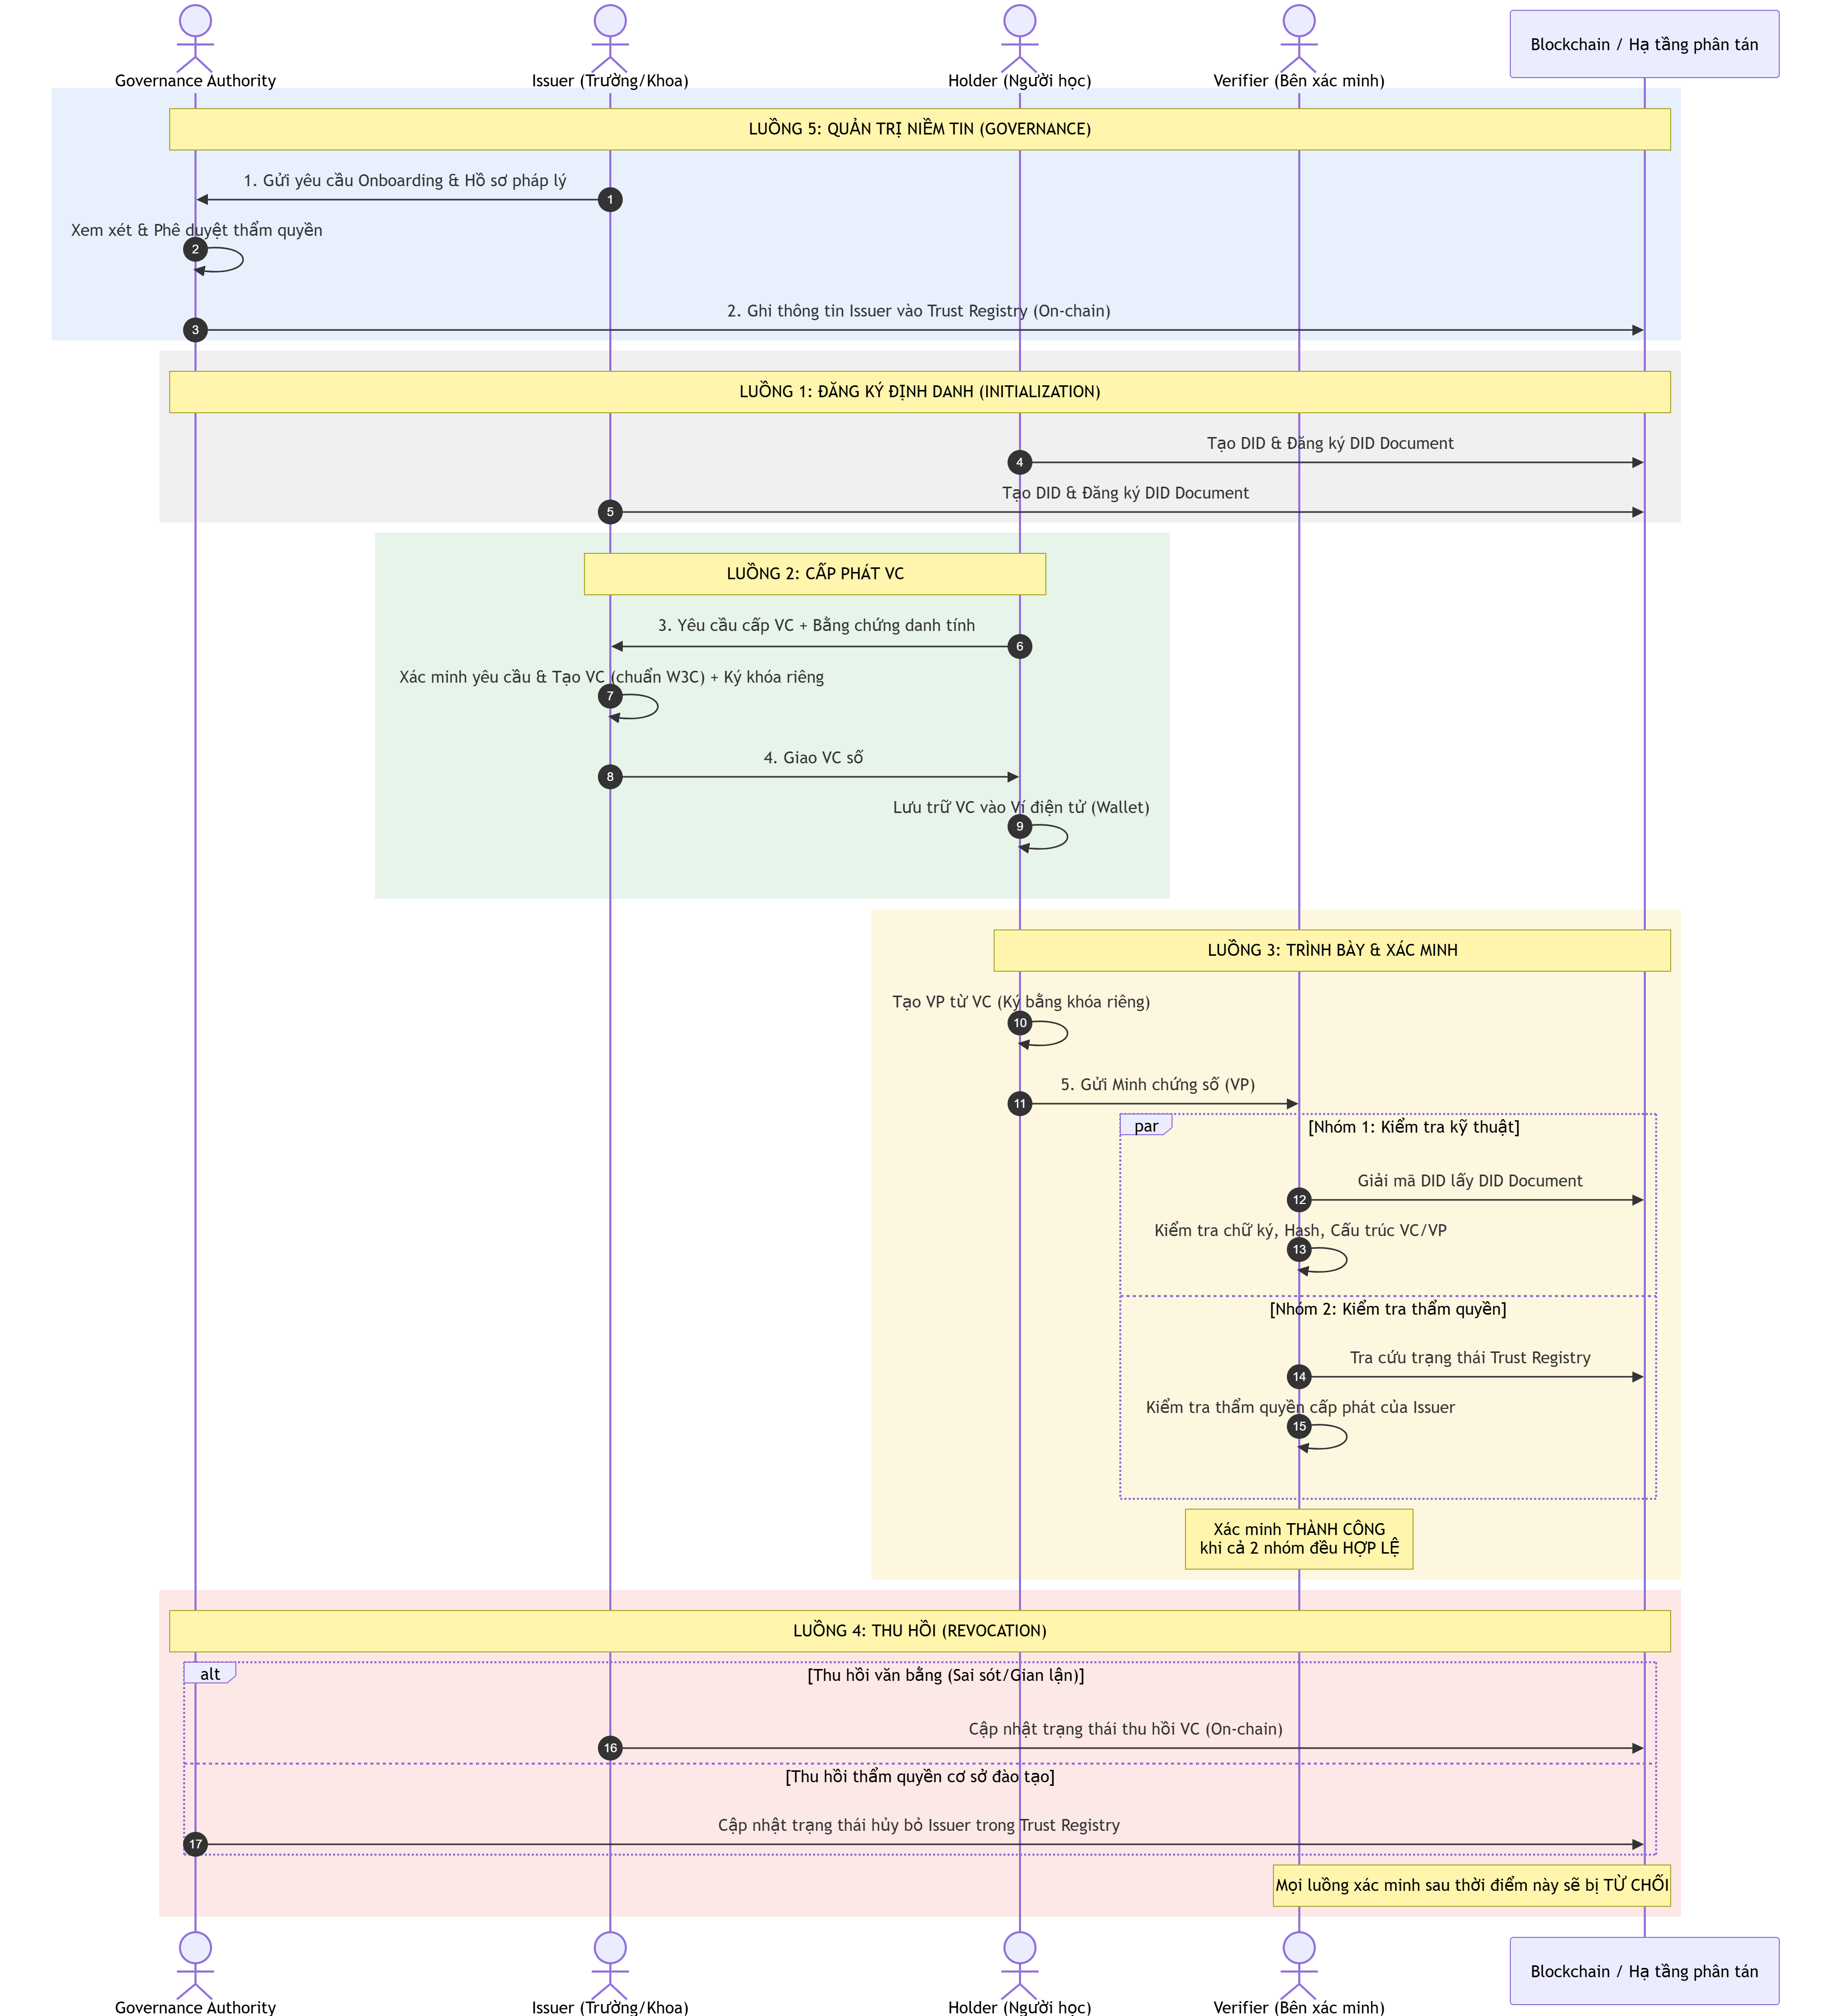
\includegraphics[width=0.75\textwidth]{images/system-flow.png}
    \caption{Luồng hoạt động tổng thể giữa bốn thực thể của hệ thống}
    \label{fig:system-workflow}
\end{figure}

\textbf{Cơ quan quản trị} (Governance Authority) là thực thể có thẩm quyền cao nhất trong hệ sinh thái. Trong bối cảnh ĐHQGHN, đây là cấp quản lý của ĐHQGHN hoặc đơn vị được ủy quyền về đảm bảo chất lượng. Cơ quan quản trị không tham gia vào luồng cấp phát hay xác minh thông thường; vai trò của nó là thiết lập và duy trì các quy tắc, cụ thể hóa qua việc quản lý sổ đăng ký tin cậy --- quyết định tổ chức nào được phép cấp phát, với phạm vi thẩm quyền nào, trong thời hạn nào, và thu hồi khi cần. Đây là nguồn niềm tin gốc của toàn hệ thống, nên khóa của nó cần mức bảo vệ cao nhất, và cơ chế chuyển quyền gốc là một điểm thiết kế quan trọng (Mục 3.4.4).

\textbf{Bên phát hành} (Issuer) là các đơn vị được cơ quan quản trị phê duyệt để cấp phát văn bằng --- các trường thành viên hoặc đơn vị đào tạo của ĐHQGHN. Mỗi bên phát hành có định danh riêng và bộ khóa riêng. Phạm vi thẩm quyền quy định những loại văn bằng mà đơn vị được phép cấp, và được ghi nhận trong sổ đăng ký tin cậy.

\textbf{Chủ thể} (Holder) là người học --- đối tượng của văn bằng, đồng thời là bên nhận và lưu giữ chứng thực trong ví định danh của mình. Chủ thể là thực thể duy nhất quyết định chia sẻ thông tin nào, với ai và khi nào.

\textbf{Bên xác minh} (Verifier) là bất kỳ bên nào cần kiểm chứng tính hợp lệ của văn bằng. Điểm quan trọng là bên xác minh không cần quan hệ đặc biệt nào với bên phát hành hay cơ quan quản trị; họ chỉ cần truy cập được hạ tầng công bố trạng thái.

\subsection{Luồng hoạt động}

Hệ thống vận hành qua năm luồng. Bốn luồng đầu tương ứng với vòng đời chứng thực; luồng thứ năm là luồng quản trị --- luồng diễn ra ít thường xuyên nhất nhưng có tác động dài hạn lớn nhất, và thường bị bỏ qua trong các mô tả về định danh tự chủ.

\noindent \textbf{Luồng 1 --- Đăng ký định danh.} Thực thể muốn tham gia hệ thống sinh cặp khóa, dựng DID Document chứa khóa công khai, ghim tài liệu đó lên lớp lưu trữ ngoài chuỗi để nhận một định danh nội dung, rồi ghi định danh cùng giá trị băm của tài liệu lên chuỗi. Sau bước này, bất kỳ ai cũng phân giải được DID để lấy khóa công khai và kiểm tra được tài liệu nhận về đúng là bản đã đăng ký.

\noindent \textbf{Luồng 2 --- Cấp phát chứng thực.} Chủ thể gửi yêu cầu cấp phát kèm bằng chứng về danh tính. Bên phát hành xác minh yêu cầu, dựng chứng thực theo chuẩn, ký bằng khóa riêng của mình, ghim nội dung lên lớp lưu trữ ngoài chuỗi, rồi ghi bản ghi neo lên chuỗi. Hợp đồng kiểm tra thẩm quyền của bên phát hành \emph{trước khi} ghi --- nghĩa là một đơn vị không có thẩm quyền sẽ thất bại ngay tại bước này, chứ không phải bị phát hiện về sau ở bước xác minh.

\noindent \textbf{Luồng 3 --- Trình bày và xác minh.} Chủ thể dựng bản trình bày từ các chứng thực mình chọn, ký bằng khóa riêng, và chuyển cho bên xác minh. Bên xác minh thực hiện một chuỗi kiểm tra gồm hai nhóm độc lập: nhóm kỹ thuật kiểm tra chữ ký và tính toàn vẹn; nhóm thẩm quyền tra cứu trạng thái của chứng thực và trạng thái của bên phát hành trên chuỗi. Chi tiết tại Mục 3.6.

\noindent \textbf{Luồng 4 --- Thu hồi chứng thực.} Khi cần thu hồi một chứng thực, bên có thẩm quyền cập nhật trạng thái trên chuỗi. Mọi lần xác minh sau đó phát hiện trạng thái này và từ chối chứng thực, dù chữ ký vẫn hợp lệ về mặt toán học.

\noindent \textbf{Luồng 5 --- Quản trị thẩm quyền.} Khi một tổ chức muốn trở thành bên phát hành, cơ quan quản trị xem xét và --- nếu phê duyệt --- ghi bản ghi thẩm quyền lên chuỗi kèm phạm vi và thời hạn. Thao tác này để lại dấu vết vĩnh viễn. Tương tự khi thu hồi: cơ quan quản trị cập nhật trạng thái, và từ thời điểm đó mọi chứng thực do đơn vị đó cấp sẽ không vượt qua bước kiểm tra thẩm quyền, dù chúng vẫn hợp lệ về mặt kỹ thuật. Điểm cần nhấn mạnh: cơ quan quản trị \emph{không} tự thực hiện thao tác này thông qua một dịch vụ trung gian --- chính người quản trị ký giao dịch từ ví của mình, và hợp đồng là bên quyết định thao tác đó có được phép hay không.

\subsection{Mô hình phân lớp}

Kiến trúc được tổ chức thành bốn lớp xếp chồng từ hạ tầng tới ứng dụng. Ba lớp đầu là các lớp kỹ thuật tương ứng với hạ tầng định danh tự chủ; lớp thứ tư là lớp quản trị.

\begin{figure}[H]
    \centering
    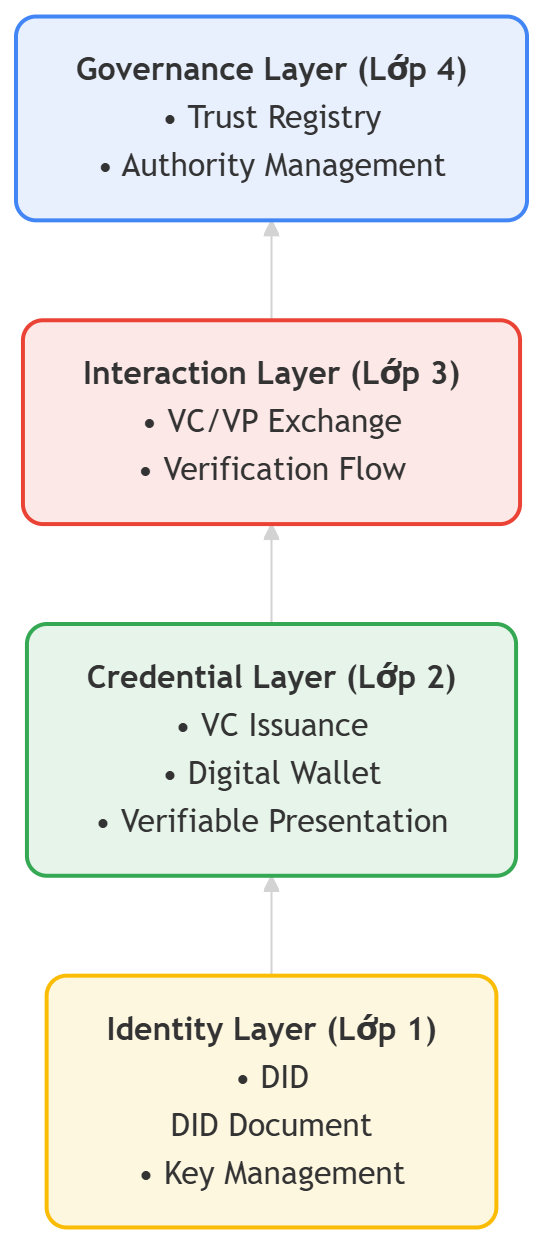
\includegraphics[width=0.3\textwidth]{images/layered_architecture.png}
    \caption{Mô hình kiến trúc phân lớp của hệ thống đề xuất}
    \label{fig:layered-architecture}
\end{figure}

\textbf{Lớp định danh} (Identity Layer) là nền của toàn hệ thống: cung cấp định danh duy nhất và bền vững cho mọi thực thể, cơ chế quản lý và xoay vòng khóa, và khả năng phân giải định danh thành thông tin kỹ thuật cần cho việc kiểm tra chữ ký.

\textbf{Lớp chứng thực} (Credential Layer) xây trên lớp định danh để thực hiện vòng đời văn bằng số: cấu trúc dữ liệu, cấp phát, lưu trữ, và quản lý trạng thái hiệu lực.

\textbf{Lớp tương tác} (Interaction Layer) định nghĩa cách các thực thể trao đổi: giao thức trình bày, quy trình xác minh, và cơ chế chia sẻ giữa các tổ chức.

\textbf{Lớp quản trị} (Governance Layer) lấp đầy khoảng trống về niềm tin thể chế và niềm tin quản trị: duy trì sổ đăng ký tin cậy, xử lý các quyết định phê duyệt và thu hồi, và cung cấp dữ liệu để lớp tương tác trả lời được câu hỏi {``}bên phát hành này có thẩm quyền hay không{''}.

Cần ghi nhận một điểm về cách trình bày. Như đã phân tích ở Mục 2.7.4, kiến trúc tham chiếu Trust over IP mô tả quản trị như một chiều xuyên suốt song song với chồng kỹ thuật, không phải một lớp riêng \cite{ToIP_GovMetamodel2022}. Cách nhìn đó chính xác hơn về mặt khái niệm, bởi các quyết định quản trị thực tế tác động tới cả bốn lớp. Nghiên cứu này vẫn trình bày quản trị thành một lớp riêng vì nó giúp mô tả rõ ranh giới trách nhiệm trong một hệ thống cụ thể, nhưng không xem đó là mô hình khái niệm đầy đủ.

\subsection{Các thành phần hệ thống}

\begin{longtable}{|p{2.8cm}|p{4.3cm}|p{2.1cm}|p{2.4cm}|p{2.4cm}|}
\caption{Các thành phần chính của hệ thống}
\label{tab:system-components} \\

\hline
\textbf{Thành phần} & \textbf{Trách nhiệm} & \textbf{Đầu vào chính} & \textbf{Đầu ra chính} & \textbf{Phụ thuộc} \\
\hline
\endfirsthead

\hline
\textbf{Thành phần} & \textbf{Trách nhiệm} & \textbf{Đầu vào chính} & \textbf{Đầu ra chính} & \textbf{Phụ thuộc} \\
\hline
\endhead

\hline
\endfoot

\hline
\endlastfoot

Sổ đăng ký định danh
& Đăng ký, cập nhật, thu hồi định danh; giữ lịch sử phiên bản DID Document
& Giá trị băm và định danh nội dung của DID Document
& Bản ghi định danh trên chuỗi
& Lớp lưu trữ ngoài chuỗi
\\ \hline

Sổ đăng ký tin cậy
& Lưu và công bố trạng thái thẩm quyền: phạm vi, thời hạn, trạng thái, phiên bản
& Địa chỉ của bên phát hành
& Bản ghi thẩm quyền trên chuỗi
& Sổ đăng ký định danh
\\ \hline

Sổ đăng ký chứng thực
& Neo giá trị băm của chứng thực và quản lý trạng thái hiệu lực
& Giá trị băm, định danh nội dung, loại và thời hạn
& Bản ghi chứng thực trên chuỗi
& Sổ đăng ký tin cậy, sổ đăng ký định danh
\\ \hline

Ví định danh số
& Sinh và bảo vệ khóa, ký chứng thực và ký giao dịch, dựng bản trình bày
& Mật khẩu hoặc cụm từ khôi phục
& Chữ ký, giao dịch đã ký, bản trình bày
& Không phụ thuộc tầng dịch vụ
\\ \hline

Tầng chuỗi phía máy khách
& Dựng giao dịch, lấy dạng tuần tự hóa từ nút đầy đủ, ký, gửi và chờ xác nhận
& Tên hàm và tham số
& Mã giao dịch đã xác nhận
& Ví định danh, nút đầy đủ
\\ \hline

Dịch vụ xác minh giao dịch
& Kiểm bốn điều kiện của giao dịch với nút đầy đủ trước khi ghi chỉ mục
& Mã giao dịch do máy khách khai báo
& Kết luận chấp nhận hoặc từ chối
& Nút đầy đủ
\\ \hline

Dịch vụ xác minh chứng thực
& Thực hiện bảy bước kiểm tra và trả báo cáo theo từng bước
& Bản trình bày
& Báo cáo xác minh chi tiết
& Toàn bộ sổ đăng ký, lớp lưu trữ ngoài chuỗi
\\ \hline

Tầng chỉ mục
& Lưu bản sao phục vụ truy vấn nhanh, nhật ký kiểm toán, dữ liệu danh sách
& Bản ghi đã được xác minh
& Kết quả truy vấn
& Cơ sở dữ liệu dùng chung
\\ \hline

Điểm vào dịch vụ
& Điều phối yêu cầu, xác thực phiên, giới hạn tần suất
& Yêu cầu HTTP
& Phản hồi theo hợp đồng giao diện
& Toàn bộ hệ thống
\\ \hline

\end{longtable}


Ba điểm về quan hệ giữa các thành phần cần được làm rõ.

Thứ nhất, \textbf{ví định danh là thành phần duy nhất vận hành hoàn toàn phía máy khách}. Toàn bộ thao tác sinh khóa, mã hóa và ký số được thực thi trong trình duyệt bằng Web Cryptography API \cite{W3C_WebCrypto} và các thư viện mật mã chạy phía máy khách; dữ liệu đã mã hóa được lưu cục bộ qua Indexed Database API \cite{W3C_IndexedDB}. Tầng dịch vụ không tham gia vào bất kỳ thao tác mật mã nào của chủ thể và không có khả năng kỹ thuật để ký thay chủ thể. Đây là điều kiện cần để tính tự chủ của chủ thể không chỉ là một tuyên bố về chính sách.

Thứ hai, \textbf{tầng chỉ mục không nằm trên đường tin cậy}. Dịch vụ chỉ mục tồn tại để trả lời nhanh các truy vấn danh sách và lịch sử; nếu nó trả về dữ liệu sai, kết quả xác minh vẫn không bị ảnh hưởng, bởi mọi kết luận về tính hợp lệ đều được kiểm lại với chuỗi và với nội dung thực. Tính chất này là hệ quả trực tiếp của Nguyên tắc 3.

Thứ ba, \textbf{các thao tác ghi trạng thái lên chuỗi đều do chính chủ thể ký}. Dịch vụ không giữ khóa của bất kỳ vai trò nào, nên nó không thể khởi tạo một thao tác thay đổi trạng thái. Vai trò của nó trong các luồng ghi là xác minh rằng giao dịch mà máy khách khai báo thực sự tồn tại và đúng như khai báo, trước khi cập nhật chỉ mục.

\begin{figure}[H]
    \centering
    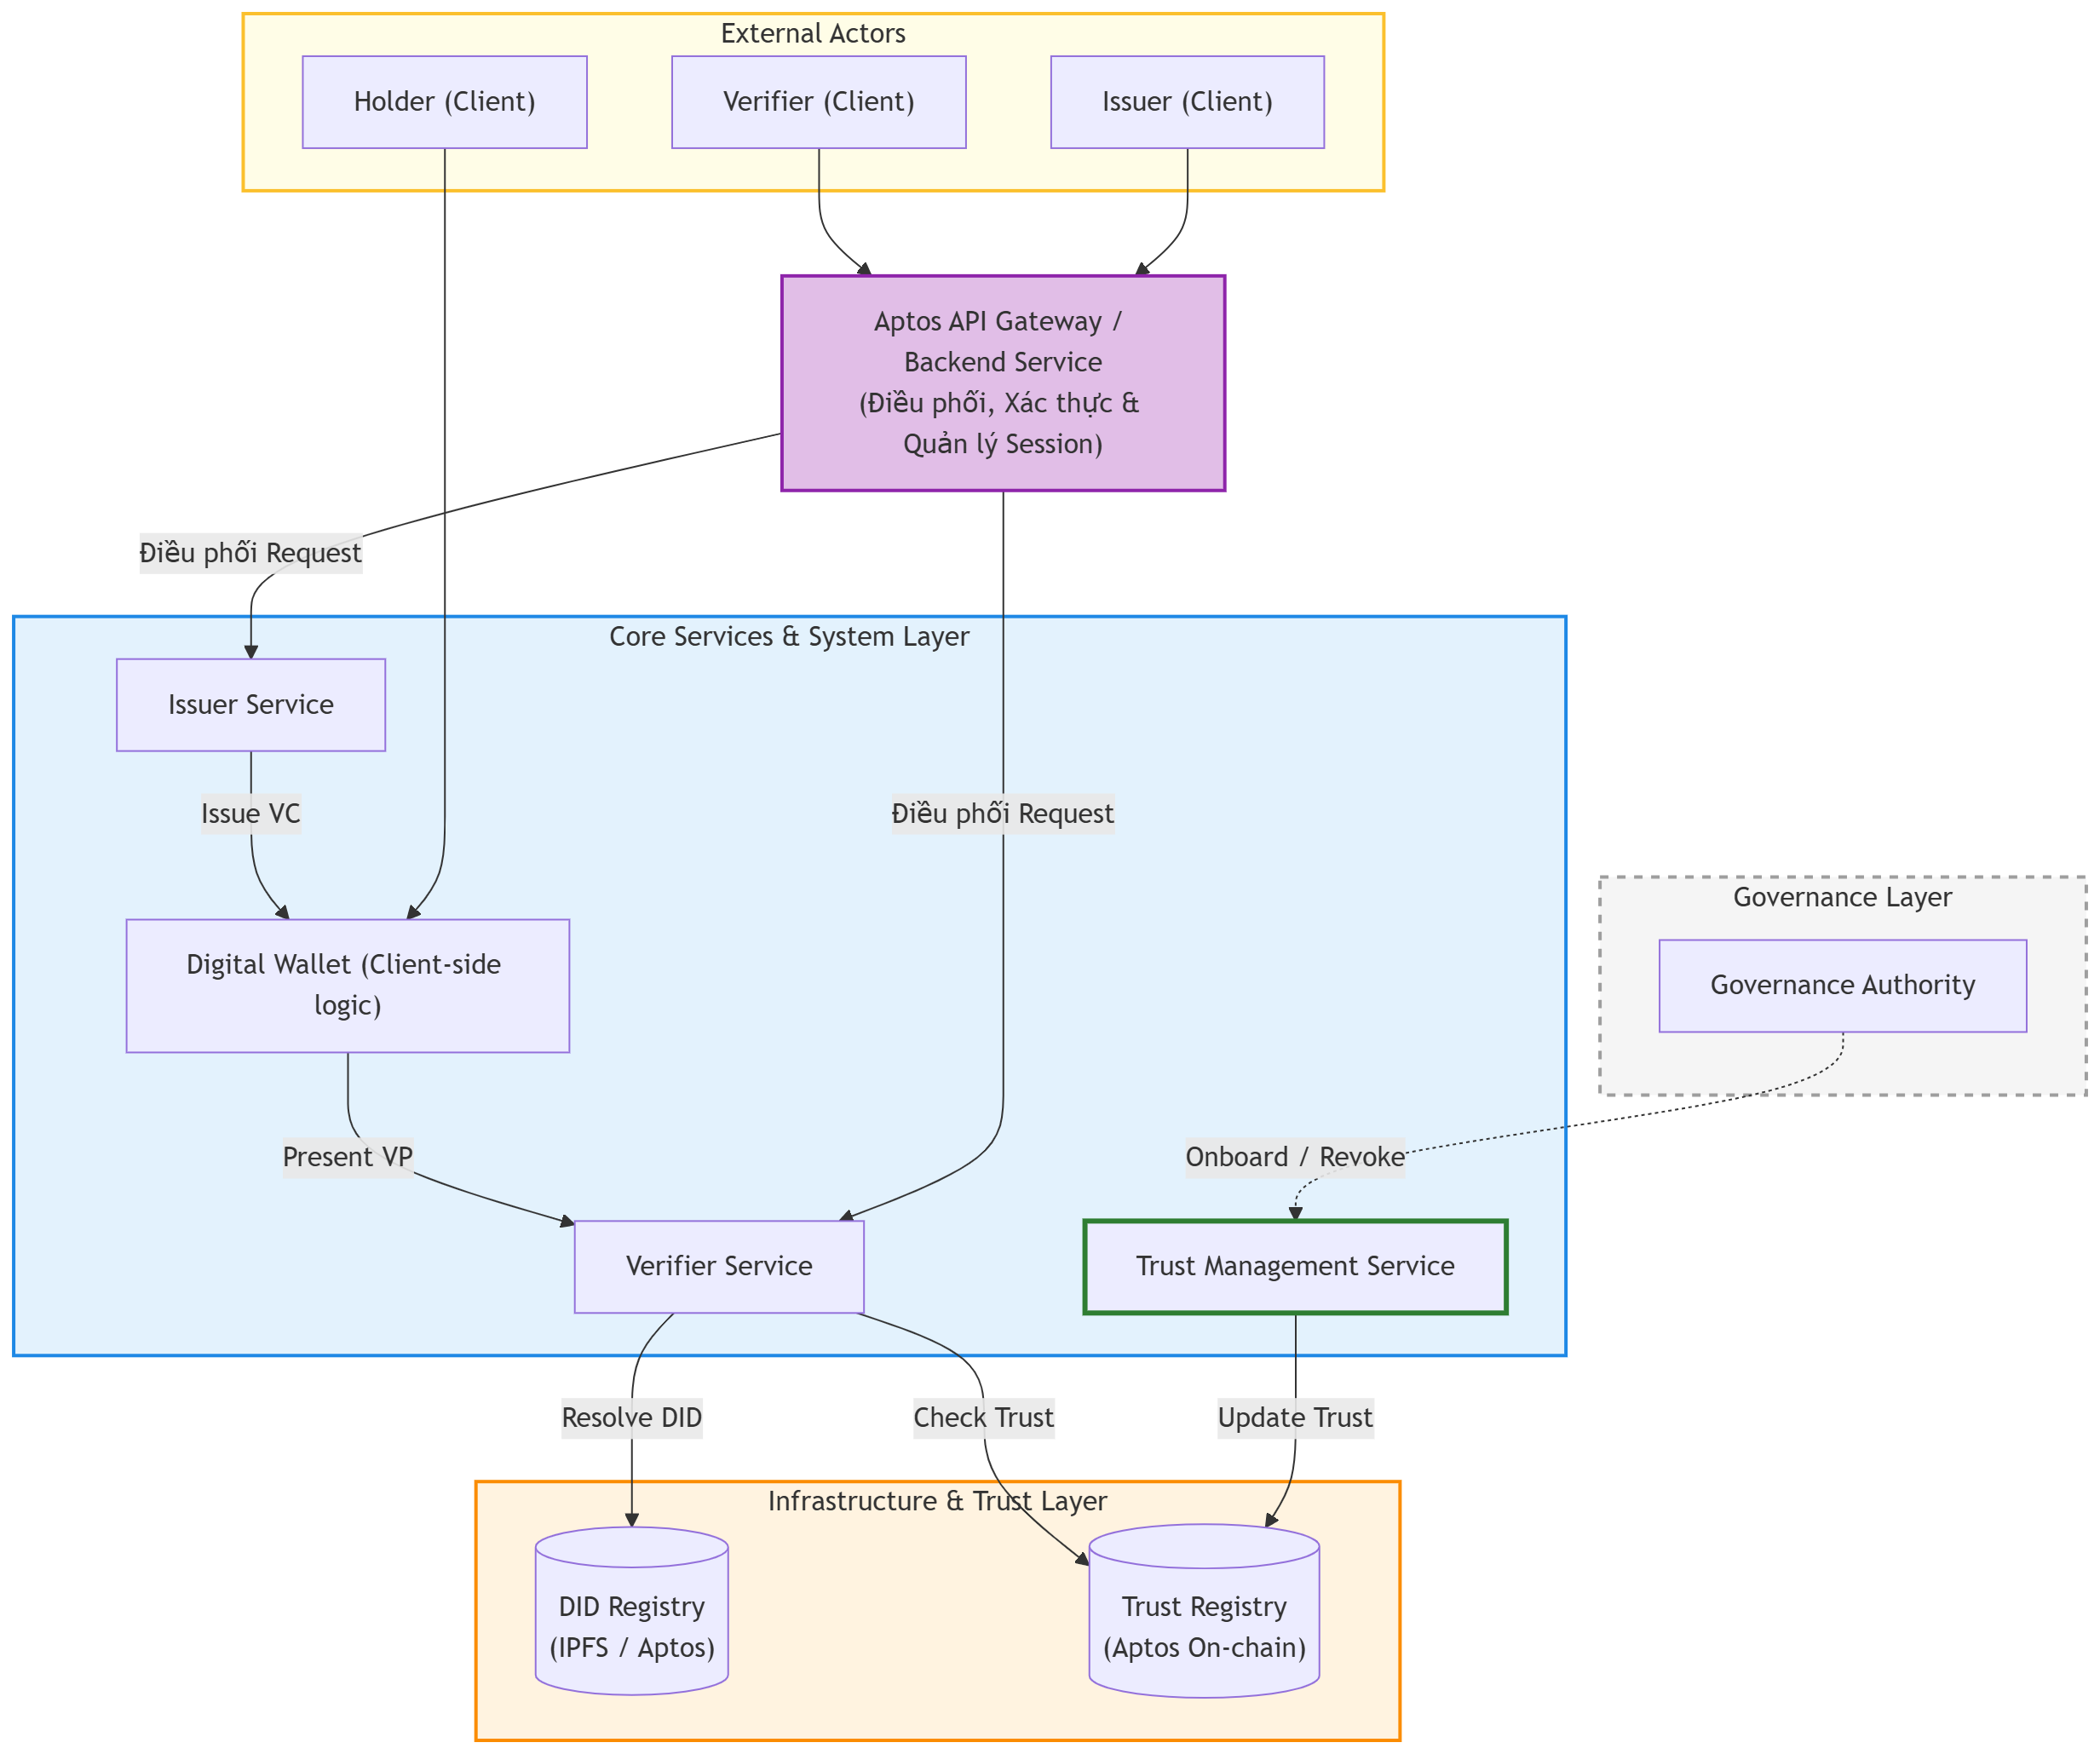
\includegraphics[width=1\textwidth]{images/system-architecture-components.png}
    \caption{Quan hệ giữa các thành phần của hệ thống}
    \label{fig:system-architecture-components}
\end{figure}

\section{Khung quản trị niềm tin}

\subsection{Vấn đề khởi tạo niềm tin}

Trước khi mô tả khung quản trị, cần xử lý một câu hỏi nền tảng mà mọi hệ thống niềm tin đều phải đối mặt: nếu mọi niềm tin đều cần được một cấp trên xác nhận, thì cấp cao nhất lấy niềm tin từ đâu?

Câu trả lời là: không lấy từ bên trong hệ thống kỹ thuật. Nguồn niềm tin gốc không thể tự chứng minh thẩm quyền của mình bằng cơ chế mật mã, bởi mọi bằng chứng mà nó tạo ra đều chỉ chứng minh rằng nó giữ một khóa cụ thể --- điều mà bất kỳ ai cũng làm được. Thẩm quyền của nguồn niềm tin gốc đến từ sự công nhận bên ngoài hệ thống: pháp lý, thể chế và xã hội. Trong trường hợp này, ĐHQGHN là nguồn niềm tin gốc không phải vì hệ thống kỹ thuật chứng minh được điều đó, mà vì ĐHQGHN được công nhận theo Luật Giáo dục đại học và có tư cách pháp nhân rõ ràng.

Nhận thức này không phải sự thừa nhận một thất bại mà là một định hướng thiết kế. Hệ thống kỹ thuật không cố thay thế sự công nhận thể chế; nó làm cho sự công nhận đó trở nên kiểm chứng được. Nói cách khác, hệ thống chuyển câu hỏi từ

\begin{quote}
{``}ĐHQGHN có đáng tin cậy hay không?{''} --- một câu hỏi thuộc phạm trù thể chế,
\end{quote}

thành

\begin{quote}
{``}Đơn vị này có đang được ĐHQGHN ủy quyền cấp loại văn bằng này hay không, và tôi có thể kiểm chứng điều đó mà không cần hỏi bất kỳ ai?{''} --- một câu hỏi trả lời được hoàn toàn bằng kỹ thuật.
\end{quote}

Đây là sự chuyển đổi mà cả tài liệu kỹ thuật của EBSI cũng nêu rõ dưới dạng nguyên tắc: sổ cái ghi nhận các quyết định về niềm tin nhưng không tạo ra chúng \cite{EBSI_TrustModel}.

\subsection{Chuỗi thẩm quyền và phạm vi cấp phát}

Khung quản trị biểu diễn thẩm quyền thành một chuỗi phân cấp có bốn mức, phản ánh đúng cấu trúc thể chế mô tả ở Mục 2.6.2.

\begin{figure}[H]
    \centering
    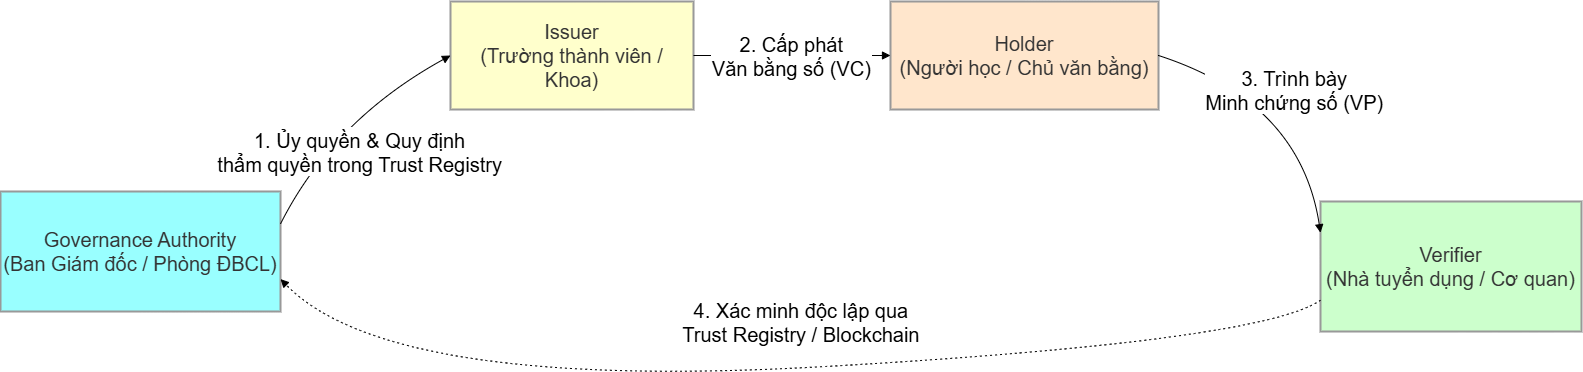
\includegraphics[width=1\textwidth]{images/system-interaction.png}
    \caption{Chuỗi niềm tin và các quan hệ ủy quyền trong hệ thống}
    \label{fig:system-interaction}
\end{figure}

Ở gốc là \textbf{quản trị viên gốc} (root), thực thể duy nhất và được xác lập tại thời điểm khởi tạo hệ thống. Quản trị viên gốc cấp quyền cho các \textbf{quản trị viên} (admin), là các đơn vị được giao nhiệm vụ quản lý việc phê duyệt bên phát hành. Quản trị viên phê duyệt các \textbf{bên phát hành} (issuer) kèm phạm vi thẩm quyền. Bên phát hành có bit ủy quyền đặc biệt có thể phê duyệt \textbf{bên phát hành cấp dưới} (sub-issuer) trong phạm vi hẹp hơn của mình (Mục 3.4.3).

Điểm thiết kế quan trọng là \textbf{cách biểu diễn phạm vi thẩm quyền}. Như đã nêu ở Mục 2.8, phần lớn hệ thống hiện có chỉ biểu diễn thẩm quyền ở dạng nhị phân. Thiết kế này dùng một mặt nạ bit để biểu diễn tập các loại văn bằng mà một đơn vị được phép cấp: mỗi loại ứng với một bit, và phạm vi thẩm quyền của đơn vị là phép hợp của các bit tương ứng.

\begin{table}[H]
\centering
\caption{Biểu diễn phạm vi thẩm quyền bằng mặt nạ bit}
\label{tab:vc-type-mask}
\renewcommand{\arraystretch}{1.25}
\begin{tabular}{|c|c|p{4.6cm}|p{5.2cm}|}
\hline
\textbf{Bit} & \textbf{Giá trị} & \textbf{Loại chứng thực} & \textbf{Ghi chú} \\
\hline
0 & 1  & Bằng cử nhân / kỹ sư & \\ \hline
1 & 2  & Bằng thạc sĩ & \\ \hline
2 & 4  & Bằng tiến sĩ & \\ \hline
3 & 8  & Bảng điểm, kết quả học tập & \\ \hline
4 & 16 & Chứng nhận vi mô, chứng chỉ ngắn hạn & \\ \hline
5 & 32 & Chứng thực ủy quyền & Chỉ quản trị viên gốc được cấp bit này; cho phép đơn vị phê duyệt bên phát hành cấp dưới \\ \hline
\end{tabular}
\end{table}

\noindent Phạm vi thẩm quyền của một đơn vị là phép hợp các giá trị tương ứng. Ví dụ, một trường được phép cấp bằng cử nhân, bằng thạc sĩ và bảng điểm có phạm vi $M = 1 \vee 2 \vee 8 = 11$. Phép kiểm tra {``}đơn vị này có được cấp loại $T$ hay không{''} rút về điều kiện $M \wedge T \neq 0$, còn phép kiểm tra {``}phạm vi $A$ là tập con của phạm vi $B$ hay không{''} rút về điều kiện $A \wedge \neg B = 0$. Cả hai đều có chi phí không đổi, không phụ thuộc số loại văn bằng trong phạm vi.


Cách biểu diễn này có ba ưu điểm thực tiễn. Thao tác kiểm tra {``}đơn vị này có được phép cấp loại văn bằng $T$ hay không{''} trở thành một phép giao bit duy nhất, nên chi phí không đổi dù phạm vi rộng hay hẹp. Thao tác kiểm tra {``}phạm vi $A$ có là tập con của phạm vi $B$ hay không{''} --- cần thiết cho việc ủy quyền lại --- cũng rút về một phép bit. Và toàn bộ phạm vi thẩm quyền được lưu trong một số nguyên duy nhất, nên không làm tăng đáng kể chi phí lưu trữ trên chuỗi. Giới hạn là số loại văn bằng tối đa bằng độ rộng của số nguyên được chọn; với một số nguyên 64 bit, giới hạn này đủ rộng cho bài toán hiện tại và có thể mở rộng bằng cách dùng nhiều từ hoặc chuyển sang sổ đăng ký loại dựa trên chuỗi định danh.

Ngoài phạm vi, mỗi bản ghi thẩm quyền còn mang \textbf{thời hạn ủy quyền}. Trường này cho phép biểu diễn đúng thực tiễn quản trị: một đơn vị được phép cấp bằng trong một chu kỳ kiểm định, và thẩm quyền tự hết hiệu lực khi chu kỳ kết thúc nếu không được gia hạn. Giá trị không được đặt tương ứng với ủy quyền vô thời hạn, hợp lý với một số loại thẩm quyền nhưng không nên là mặc định.

\subsection{Ủy quyền nhiều cấp}

Một yêu cầu thực tiễn mà các hệ thống hiện có chưa xử lý --- và như đã nêu ở Mục 2.6.3, chính đặc tả chuẩn hóa còn hoãn sang phiên bản sau --- là ủy quyền nhiều cấp: một trường thành viên được ĐHQGHN ủy quyền có thể cần ủy quyền tiếp cho một khoa hoặc một đơn vị trực thuộc.

Nếu cho phép ủy quyền lại không giới hạn, chuỗi thẩm quyền sẽ mất ý nghĩa: một đơn vị được phép cấp bằng cử nhân có thể ủy quyền cho đơn vị khác quyền cấp bằng tiến sĩ, hoặc ủy quyền với thời hạn dài hơn thời hạn của chính mình. Vì vậy thiết kế đặt ba ràng buộc, và cả ba được thi hành bởi hợp đồng chứ không bởi quy trình hành chính:

\begin{itemize}
    \item \textbf{Phạm vi phải là tập con.} Phạm vi mà bên ủy quyền trao cho cấp dưới phải là tập con của phạm vi mà chính họ đang có. Không thể trao thứ mình không có.
    \item \textbf{Thời hạn không được vượt quá thời hạn của bên ủy quyền.} Một ủy quyền phái sinh không thể sống lâu hơn ủy quyền gốc của nó.
    \item \textbf{Bit ủy quyền không được truyền tiếp.} Bên phát hành cấp dưới không nhận được quyền ủy quyền lại. Ràng buộc này giới hạn độ sâu của chuỗi ở hai cấp, và đó là lựa chọn có chủ đích: một chuỗi ủy quyền sâu không giới hạn khiến việc truy vết trách nhiệm trở nên bất khả thi trong thực tế, trong khi lợi ích thu được không rõ ràng. Riêng bit ủy quyền chỉ quản trị viên gốc được cấp.
\end{itemize}

Mỗi quan hệ ủy quyền còn được gắn với một \emph{chứng thực ủy quyền} --- một chứng thực do bên ủy quyền ký, xác nhận phạm vi được trao. Nội dung chứng thực được lưu ngoài chuỗi và giá trị băm cùng định danh nội dung của nó được ghi vào bản ghi thẩm quyền. Nhờ đó bên xác minh có thể truy xuất và kiểm tra bằng chứng về quan hệ ủy quyền, chứ không chỉ đọc một cờ trạng thái. Để tránh biến yêu cầu này thành gánh nặng vô ích, hợp đồng chỉ bắt buộc có chứng thực ủy quyền khi thực sự có quan hệ ủy quyền --- tức khi đơn vị được cấp bit ủy quyền, hoặc khi chính nó được phê duyệt bởi một bên phát hành chứ không phải bởi quản trị viên.

\subsection{Chuyển quyền gốc gồm hai bước}

Quản trị viên gốc là điểm tập trung quyền lực duy nhất của hệ thống, nên cơ chế chuyển quyền gốc là một điểm thiết kế có hệ quả đặc biệt lớn. Thiết kế trực quan nhất --- một thao tác duy nhất trong đó quản trị viên gốc hiện tại chỉ định địa chỉ của người kế nhiệm --- có một khuyết điểm nghiêm trọng mà chỉ bộc lộ khi đã quá muộn: nó không có cơ chế nào kiểm tra rằng địa chỉ đích thực sự có người kiểm soát.

Nếu địa chỉ đích bị gõ sai, hoặc thuộc về một khóa đã mất, quyền quản trị gốc chuyển tới một địa chỉ không ai điều khiển được. Hệ thống không hỏng ngay --- các thao tác cấp phát và xác minh vẫn chạy bình thường --- nhưng toàn bộ năng lực quản trị bị mất vĩnh viễn: không thể phê duyệt bên phát hành mới, không thể thu hồi bên phát hành cũ, và không thể sửa chính sai sót đó. Vì trạng thái trên chuỗi là bất biến, không có cách khắc phục nào ngoài việc triển khai lại toàn bộ hệ thống ở một địa chỉ mới.

Thiết kế vì vậy tách thao tác này thành hai bước:

\begin{enumerate}
    \item \textbf{Đề cử.} Quản trị viên gốc hiện tại ghi địa chỉ của người được đề cử vào trạng thái chờ. Quyền quản trị \emph{chưa} chuyển.
    \item \textbf{Ký nhận.} Người được đề cử tự ký một giao dịch để tiếp nhận. Chỉ khi giao dịch này thành công thì quyền mới chuyển.
\end{enumerate}

Cùng với đó là thao tác thứ ba --- \textbf{hủy đề cử} --- cho phép quản trị viên gốc rút lại đề cử trước khi nó được tiếp nhận.

Giá trị của thiết kế này nằm ở bước thứ hai, và chính xác hơn là ở \emph{bản chất của chữ ký} trong bước đó. Chữ ký của người được đề cử là bằng chứng mật mã duy nhất cho thấy họ thực sự kiểm soát khóa riêng tương ứng với địa chỉ đã nêu --- điều mà một thao tác một bước không bao giờ chứng minh được. Đây là một trường hợp cụ thể của một nguyên tắc tổng quát hơn: khi một thao tác không thể hoàn tác, điều kiện tiên quyết của nó phải được chứng minh bằng hành động của bên bị ảnh hưởng, không phải bằng khai báo của bên thực hiện.

\subsection{Nguyên tắc bất đối xứng giữa cấp và thu hồi}

Nguyên tắc thiết kế thứ hai được rút ra trong quá trình xây dựng hệ thống liên quan tới quan hệ giữa thao tác cấp và thao tác thu hồi.

Cách thiết kế tự nhiên là đối xứng: nếu một đơn vị cần thẩm quyền còn hiệu lực để cấp văn bằng, thì nó cũng cần thẩm quyền còn hiệu lực để thu hồi văn bằng. Logic nghe hợp lý nhưng dẫn tới một kết quả sai trong tình huống quan trọng nhất.

Xét kịch bản sau. Một trường thành viên có thẩm quyền cấp bằng đến hết năm 2026. Năm 2027, trường phát hiện một văn bằng mình đã cấp năm 2025 là kết quả của gian lận. Với thiết kế đối xứng, trường không thu hồi được văn bằng đó, vì thẩm quyền của họ đã hết hạn. Văn bằng gian lận tiếp tục vượt qua mọi phép xác minh. Tình huống tương tự xảy ra khi thẩm quyền của một đơn vị bị thu hồi vì phát hiện sai phạm --- đúng lúc cần thu hồi các văn bằng đã cấp nhất thì năng lực thu hồi lại bị khóa.

Phân tích này dẫn tới nguyên tắc: \textbf{thao tác thu hồi luôn phải dễ hơn thao tác cấp}. Cụ thể, trong thiết kế:

\begin{itemize}
    \item Cấp phát chứng thực đòi hỏi thẩm quyền \emph{còn hiệu lực} và loại văn bằng nằm \emph{trong phạm vi} được phép.
    \item Thu hồi chứng thực chỉ đòi hỏi \emph{quyền sở hữu} --- bên thu hồi đúng là bên đã cấp chứng thực đó --- và định danh của bên đó còn hoạt động. Không kiểm tra thẩm quyền còn hiệu lực, không kiểm tra phạm vi.
    \item Một chứng thực đã hết hạn vẫn thu hồi được. Điều này thoạt nghe vô nghĩa, nhưng thu hồi và hết hạn mang hai thông điệp khác nhau: hết hạn nói rằng chứng thực không còn giá trị \emph{từ thời điểm nào đó}; thu hồi nói rằng chứng thực \emph{chưa bao giờ} đáng tin. Thông điệp thứ hai cần được phát ra kể cả khi chứng thực đã hết hạn, vì nó là một tuyên bố vĩnh viễn về gian lận.
\end{itemize}

Nguyên tắc này có một phát biểu tổng quát: trong hệ thống an toàn, các thao tác làm giảm quyền hoặc giảm độ tin cậy nên có điều kiện tiên quyết lỏng hơn các thao tác làm tăng chúng. Điều kiện chặt ở thao tác giảm không bảo vệ hệ thống mà chỉ ngăn hệ thống tự sửa lỗi.

\subsection{Dấu vết kiểm toán và khôi phục vai trò}

Hai yêu cầu đối lập cần được xử lý cùng nhau: mọi thay đổi quản trị phải để lại dấu vết không thể xóa, và một đơn vị bị thu hồi thẩm quyền phải có thể được cấp lại sau khi khắc phục sai phạm.

Nếu bản ghi thẩm quyền bị ghi đè khi cấp lại, dấu vết kiểm toán sẽ mất. Nếu không cho cấp lại, hệ thống không phản ánh được thực tiễn --- một đơn vị bị đình chỉ rồi được phục hồi sau kiểm định là tình huống bình thường. Thiết kế giải quyết bằng cách tách hai thứ: bảng tra cứu {``}đơn vị $A$ hiện ứng với bản ghi nào{''} được cập nhật, còn bản ghi cũ vẫn nằm nguyên trong tập các bản ghi. Mỗi bản ghi mang một số \textbf{phiên bản} tăng dần theo mỗi lần được cấp lại. Nhờ đó lịch sử đầy đủ của một đơn vị --- được cấp quyền lần nào, bị thu hồi khi nào vì lý do gì, được phục hồi khi nào --- đều truy xuất được, trong khi truy vấn trạng thái hiện tại vẫn là một phép tra cứu trực tiếp.

Cơ chế tương tự áp dụng cho định danh. Khi khóa riêng của một thực thể bị lộ, hành động đúng là thu hồi định danh cũ và đăng ký định danh mới bằng khóa mới. Nếu hệ thống khóa một địa chỉ vào đúng một định danh vĩnh viễn, thì sự cố lộ khóa đồng nghĩa với mất địa chỉ vĩnh viễn. Thiết kế cho phép đăng ký định danh mới sau khi định danh cũ đã bị thu hồi, đồng thời giữ định danh cũ trong sổ với trạng thái đã thu hồi --- để các chứng thực được cấp bằng khóa cũ vẫn tra cứu được và vẫn phản ánh đúng trạng thái.

\subsection{Phân tách thẩm quyền theo thao tác}

Một nội dung của khung quản trị là việc quy định thao tác nào thuộc vai trò nào. Các quy định này không phải lựa chọn tùy ý mà xuất phát từ yêu cầu phân tách trách nhiệm.

\begin{longtable}{|p{4.3cm}|p{3.2cm}|p{6.5cm}|}
\caption{Phân tách thẩm quyền theo thao tác}
\label{tab:role-permission} \\

\hline
\textbf{Thao tác} & \textbf{Vai trò được phép} & \textbf{Cơ sở của quy định} \\
\hline
\endfirsthead

\hline
\textbf{Thao tác} & \textbf{Vai trò được phép} & \textbf{Cơ sở của quy định} \\
\hline
\endhead

\hline
\endfoot

\hline
\endlastfoot

Cấp và thu hồi quyền quản trị viên
& Chỉ quản trị viên gốc
& Quyền phê duyệt bên phát hành là quyền có hệ quả rộng nhất, nên việc trao quyền đó phải tập trung ở gốc
\\ \hline

Cấp bit ủy quyền cho bên phát hành
& Chỉ quản trị viên gốc
& Bit này cho phép mở rộng chuỗi thẩm quyền; nếu quản trị viên cấp được thì chuỗi có thể mở rộng ngoài kiểm soát của gốc
\\ \hline

Phê duyệt bên phát hành (không kèm bit ủy quyền)
& Quản trị viên gốc, quản trị viên
& Đây là thao tác quản trị thường xuyên, cần phân cấp để vận hành được
\\ \hline

Phê duyệt bên phát hành cấp dưới
& Bên phát hành có bit ủy quyền
& Phạm vi phải là tập con, thời hạn không vượt thời hạn của bên ủy quyền, bit ủy quyền không truyền tiếp
\\ \hline

Đình chỉ, kích hoạt lại, thu hồi bên phát hành
& Quản trị viên gốc, quản trị viên
& Thao tác làm giảm quyền, nên điều kiện tiên quyết lỏng hơn thao tác cấp
\\ \hline

Đề cử người nhận quyền gốc; hủy đề cử
& Chỉ quản trị viên gốc
& Chỉ gốc hiện tại mới có quyền quyết định người kế nhiệm
\\ \hline

Ký nhận quyền gốc
& Địa chỉ đang được đề cử, không chặn theo vai trò
& Tại thời điểm ký nhận, người được đề cử chưa phải gốc; rào chắn thật là điều kiện trùng khớp địa chỉ trong hợp đồng
\\ \hline

Cấp phát chứng thực
& Bên phát hành đang hoạt động, loại nằm trong phạm vi
& Yêu cầu đầy đủ nhất trong hệ thống: cần cả thẩm quyền còn hiệu lực và phạm vi phù hợp
\\ \hline

Thu hồi chứng thực
& Bên đã cấp chứng thực đó
& Chỉ cần quyền sở hữu; không kiểm thẩm quyền còn hiệu lực, theo nguyên tắc bất đối xứng ở Mục 3.4.5
\\ \hline

Đình chỉ chứng thực
& Bên đã cấp chứng thực đó
& Thao tác tạm thời, thuộc quyền của đơn vị cấp
\\ \hline

Kích hoạt lại chứng thực bị đình chỉ
& Chỉ quản trị viên gốc, quản trị viên
& Nếu bên phát hành tự đình chỉ rồi tự kích hoạt lại, thao tác đình chỉ mất giá trị kiểm toán
\\ \hline

Đình chỉ, kích hoạt lại định danh của chính mình
& Chủ sở hữu định danh
& Tự khóa thì tự mở được; hệ thống ghi nhận ai đã đặt trạng thái đình chỉ để phân biệt với trường hợp bị quản trị viên khóa
\\ \hline

Đình chỉ, thu hồi định danh của người khác
& Quản trị viên gốc, quản trị viên
& Định danh bị quản trị viên khóa thì phải quản trị viên mở, tránh việc đối tượng bị xử lý tự giải khóa
\\ \hline

\end{longtable}


Hai quy định cần giải thích thêm. Thứ nhất, \textbf{thao tác kích hoạt lại một chứng thực bị đình chỉ chỉ thuộc quản trị viên}, không thuộc bên phát hành --- dù chính bên phát hành đã thực hiện việc đình chỉ. Lý do: nếu một đơn vị tự đình chỉ rồi tự kích hoạt lại, thao tác đình chỉ không còn giá trị kiểm toán nào, vì nó có thể được hoàn tác bất kỳ lúc nào mà không ai biết. Thứ hai, \textbf{thao tác ký nhận quyền gốc không bị chặn theo vai trò}, bởi tại đúng thời điểm ký nhận, người được đề cử vẫn chưa phải quản trị viên gốc. Chặn theo vai trò ở đó sẽ khóa đúng bước duy nhất chứng minh được họ giữ khóa riêng. Rào chắn thật vẫn nguyên: thao tác chỉ thành công trên chuỗi nếu người ký đúng là địa chỉ đang được đề cử.

\section{Mô hình dữ liệu trên chuỗi và ngoài chuỗi}

\subsection{Nguyên tắc phân chia dữ liệu}

Việc quyết định dữ liệu nào lên chuỗi và dữ liệu nào ở ngoài chuỗi không chỉ là bài toán tối ưu chi phí mà là một quyết định có ràng buộc pháp lý. Nguyên tắc áp dụng:

\begin{itemize}
    \item \textbf{Lên chuỗi:} những dữ liệu cần tính bất biến và khả năng đọc không cần xin phép, và không chứa dữ liệu cá nhân. Cụ thể gồm: định danh, giá trị băm và định danh nội dung của DID Document; bản ghi thẩm quyền của bên phát hành cùng phạm vi, thời hạn, trạng thái; giá trị băm của chứng thực, định danh nội dung của nó và trạng thái hiệu lực. Mọi trường trong nhóm này đều là giá trị băm, định danh kỹ thuật, cờ trạng thái hoặc dấu thời gian.
    \item \textbf{Ngoài chuỗi:} nội dung đầy đủ của DID Document và của chứng thực, tức những dữ liệu có khối lượng lớn hoặc chứa thông tin cá nhân.
\end{itemize}

Việc giảm tối đa dữ liệu ghi lên chuỗi là yêu cầu bắt buộc, không phải lựa chọn. Hạ tầng công khai bất biến về bản chất không hỗ trợ việc xóa, nên dữ liệu ghi lên đó không thể bị thu hồi khi chủ thể dữ liệu thực hiện quyền của mình theo Luật Bảo vệ dữ liệu cá nhân \cite{LuatBVDLCN2025}. Đây cũng là lý do thiết kế lưu giá trị băm của \emph{định danh} chứng thực chứ không lưu bản thân định danh đó: giá trị băm đủ để tra cứu nhưng không tiết lộ định danh cho người quan sát ngẫu nhiên.

\noindent \textbf{Phát biểu đúng mức về tính chất đạt được}

Một lập luận thường gặp trong lĩnh vực --- và là lập luận mà bản thiết kế này ban đầu dựa vào --- là: vì mọi trường trên chuỗi đều là giá trị băm, định danh kỹ thuật, cờ trạng thái hoặc dấu thời gian, nên không có dữ liệu cá nhân trên chuỗi. Lập luận này \textbf{không đứng vững}, và lý do đã được phân tích tại Mục 2.5.4: theo cách giải thích hiện hành của cơ quan bảo vệ dữ liệu, dữ liệu đã băm vẫn là dữ liệu cá nhân, và giá trị băm không có muối không đủ bảo đảm mức bảo mật cần thiết trên một chuỗi công khai \cite{EDPB2025}.

Trong kiến trúc này có một lý do kỹ thuật cụ thể khiến kết luận đó đúng. Giá trị băm của nội dung chứng thực \emph{buộc phải} không có muối, vì bên xác minh cần tính lại được nó từ nội dung họ nhận --- đó chính là cơ chế của bước xác minh thứ sáu. Nhưng điều đó biến giá trị băm thành một máy xác nhận: ai có một nội dung dự đoán cũng kiểm được nó có khớp bản đã neo hay không. Với dữ liệu văn bằng, không gian giá trị của các trường là hẹp, nên khả năng dò theo từ điển là có thật. Ngoài ra, địa chỉ tài khoản của chủ thể xuất hiện trong bản ghi chứng thực là một định danh giả danh có thể liên kết được với một con người cụ thể nếu người quan sát có thêm thông tin phụ.

Vì vậy tính chất mà thiết kế này đạt được cần được phát biểu như sau: kiến trúc \textbf{giảm đáng kể mức phơi nhiễm} dữ liệu cá nhân so với việc ghi nội dung trực tiếp lên chuỗi, và loại bỏ khả năng đọc trực tiếp thông tin học thuật từ dữ liệu trên chuỗi. Nó \textbf{không} bảo đảm quyền xóa dữ liệu, và không nên được trình bày như đã bảo đảm. Hai hướng xử lý triệt để --- cam kết có khóa mà khóa có thể bị tiêu hủy, hoặc chuyển sang chuỗi được cấp phép nơi vai trò bên kiểm soát dữ liệu xác định được --- đều nằm ngoài phạm vi bản thử nghiệm và được nêu tại Mục 5.4.

\subsection{Chính sách bảo vệ dữ liệu ngoài chuỗi}

\begin{longtable}{|p{3.2cm}|p{2.6cm}|p{3.1cm}|p{4.5cm}|}
\caption{Chính sách bảo vệ các loại dữ liệu lưu ngoài chuỗi}
\label{tab:encryption-policy}
\\
\hline
\textbf{Loại dữ liệu} & \textbf{Mức bảo vệ trong thiết kế} & \textbf{Trạng thái trong bản thử nghiệm} & \textbf{Cơ sở} \\
\hline
\endfirsthead

\hline
\textbf{Loại dữ liệu} & \textbf{Mức bảo vệ trong thiết kế} & \textbf{Trạng thái trong bản thử nghiệm} & \textbf{Cơ sở} \\
\hline
\endhead

\hline
\endfoot

\hline
\endlastfoot

DID Document
& Không mã hóa
& Không mã hóa, đúng thiết kế
& Theo đặc tả, tài liệu này là thông tin công khai và chỉ chứa khóa công khai cùng điểm cuối dịch vụ; không chứa dữ liệu cá nhân
\\ \hline

Chứng thực ủy quyền
& Không mã hóa
& Không mã hóa, đúng thiết kế
& Là bằng chứng về quan hệ ủy quyền giữa hai tổ chức, cần công khai để bên xác minh kiểm chứng được
\\ \hline

Nội dung chứng thực văn bằng
& Mã hóa bằng khóa công khai của chủ thể trước khi ghim
& \textbf{Chưa triển khai}: hiện ghim ở dạng không mã hóa
& Chứa dữ liệu định danh cá nhân. Hạn chế này được ghi nhận tại Mục 3.5.2 và Mục 5.3
\\ \hline

Bản trình bày
& Mã hóa hoặc giới hạn truy cập theo liên kết chia sẻ có thời hạn
& Giới hạn bằng liên kết chia sẻ có thời hạn và có thể thu hồi
& Bản trình bày được tạo cho một lần xác minh cụ thể, nên vòng đời ngắn là biện pháp giảm nhẹ hợp lý
\\ \hline

Khóa riêng của chủ thể
& Không bao giờ rời khỏi thiết bị
& Mã hóa AES-256-GCM, khóa dẫn xuất bằng PBKDF2-HMAC-SHA256, chỉ lưu bản mã trên thiết bị
& Mục 2.4.3
\\ \hline

\end{longtable}


Cần nói rõ một giới hạn của bản thử nghiệm. Trong thiết kế đầy đủ, nội dung chứng thực cần được mã hóa bằng khóa công khai của chủ thể trước khi ghim lên lớp lưu trữ ngoài chuỗi, bởi lớp lưu trữ này là công khai và việc biết được định danh nội dung đồng nghĩa với việc đọc được nội dung. Bản thử nghiệm hiện ghim nội dung chứng thực ở dạng không mã hóa, nên mô hình an toàn thực tế dựa trên việc định danh nội dung không được công bố --- một dạng bảo mật dựa trên sự khó đoán, không phải bảo mật bằng mật mã. Đây là một hạn chế thật, được ghi nhận tại Mục 5.3 chứ không được trình bày như đã giải quyết.

\subsection{Thiết kế phương thức định danh \texttt{did:vnu}}

Phương thức \cbox{did:vnu} được thiết kế cho bối cảnh nghiên cứu, với cú pháp tuân theo đặc tả W3C DID Core \cite{W3C_DIDCore2022}:

\begin{lstlisting}
    did:vnu:<loai-thuc-the>:<dia-chi-tai-khoan>
\end{lstlisting}

Trong đó \cbox{loai-thuc-the} nhận một trong các giá trị tương ứng với bốn vai trò, và \cbox{dia-chi-tai-khoan} là địa chỉ tài khoản trên chuỗi của chủ thể. Ví dụ:

\begin{lstlisting}
    did:vnu:holder:0x8f3a...4b5c
    did:vnu:issuer:0x1a2b...ef12
    did:vnu:root:0xe14d...50f4
\end{lstlisting}

Việc ánh xạ phần định danh với địa chỉ tài khoản trên chuỗi mang lại một tính chất quan trọng: chủ thể kiểm soát được định danh của mình bằng chính cặp khóa mà họ dùng để ký giao dịch, nên không cần quản lý hai bộ khóa cho hai mục đích. Tuy nhiên tính chất này cũng tạo ra một ràng buộc cần được ghi nhận: thành phần \cbox{loai-thuc-the} nằm trong chuỗi định danh, nên khi một thực thể thay đổi vai trò --- chẳng hạn một người học được phê duyệt làm bên phát hành --- định danh cũ không tự động phản ánh vai trò mới. Thiết kế xử lý bằng cách coi thành phần này là một nhãn mô tả thời điểm đăng ký, còn thẩm quyền thực tế luôn được tra cứu từ sổ đăng ký trên chuỗi theo địa chỉ. Hệ quả là giá trị của nhãn không bao giờ được dùng làm căn cứ phân quyền.

Quy trình phân giải gồm bốn bước: tách địa chỉ từ chuỗi định danh; truy vấn hợp đồng để lấy định danh nội dung, giá trị băm, phiên bản và trạng thái; tải tài liệu từ lớp lưu trữ ngoài chuỗi theo định danh nội dung; và tính lại giá trị băm của tài liệu để đối chiếu với giá trị đã neo.

\begin{figure}[H]
    \centering
    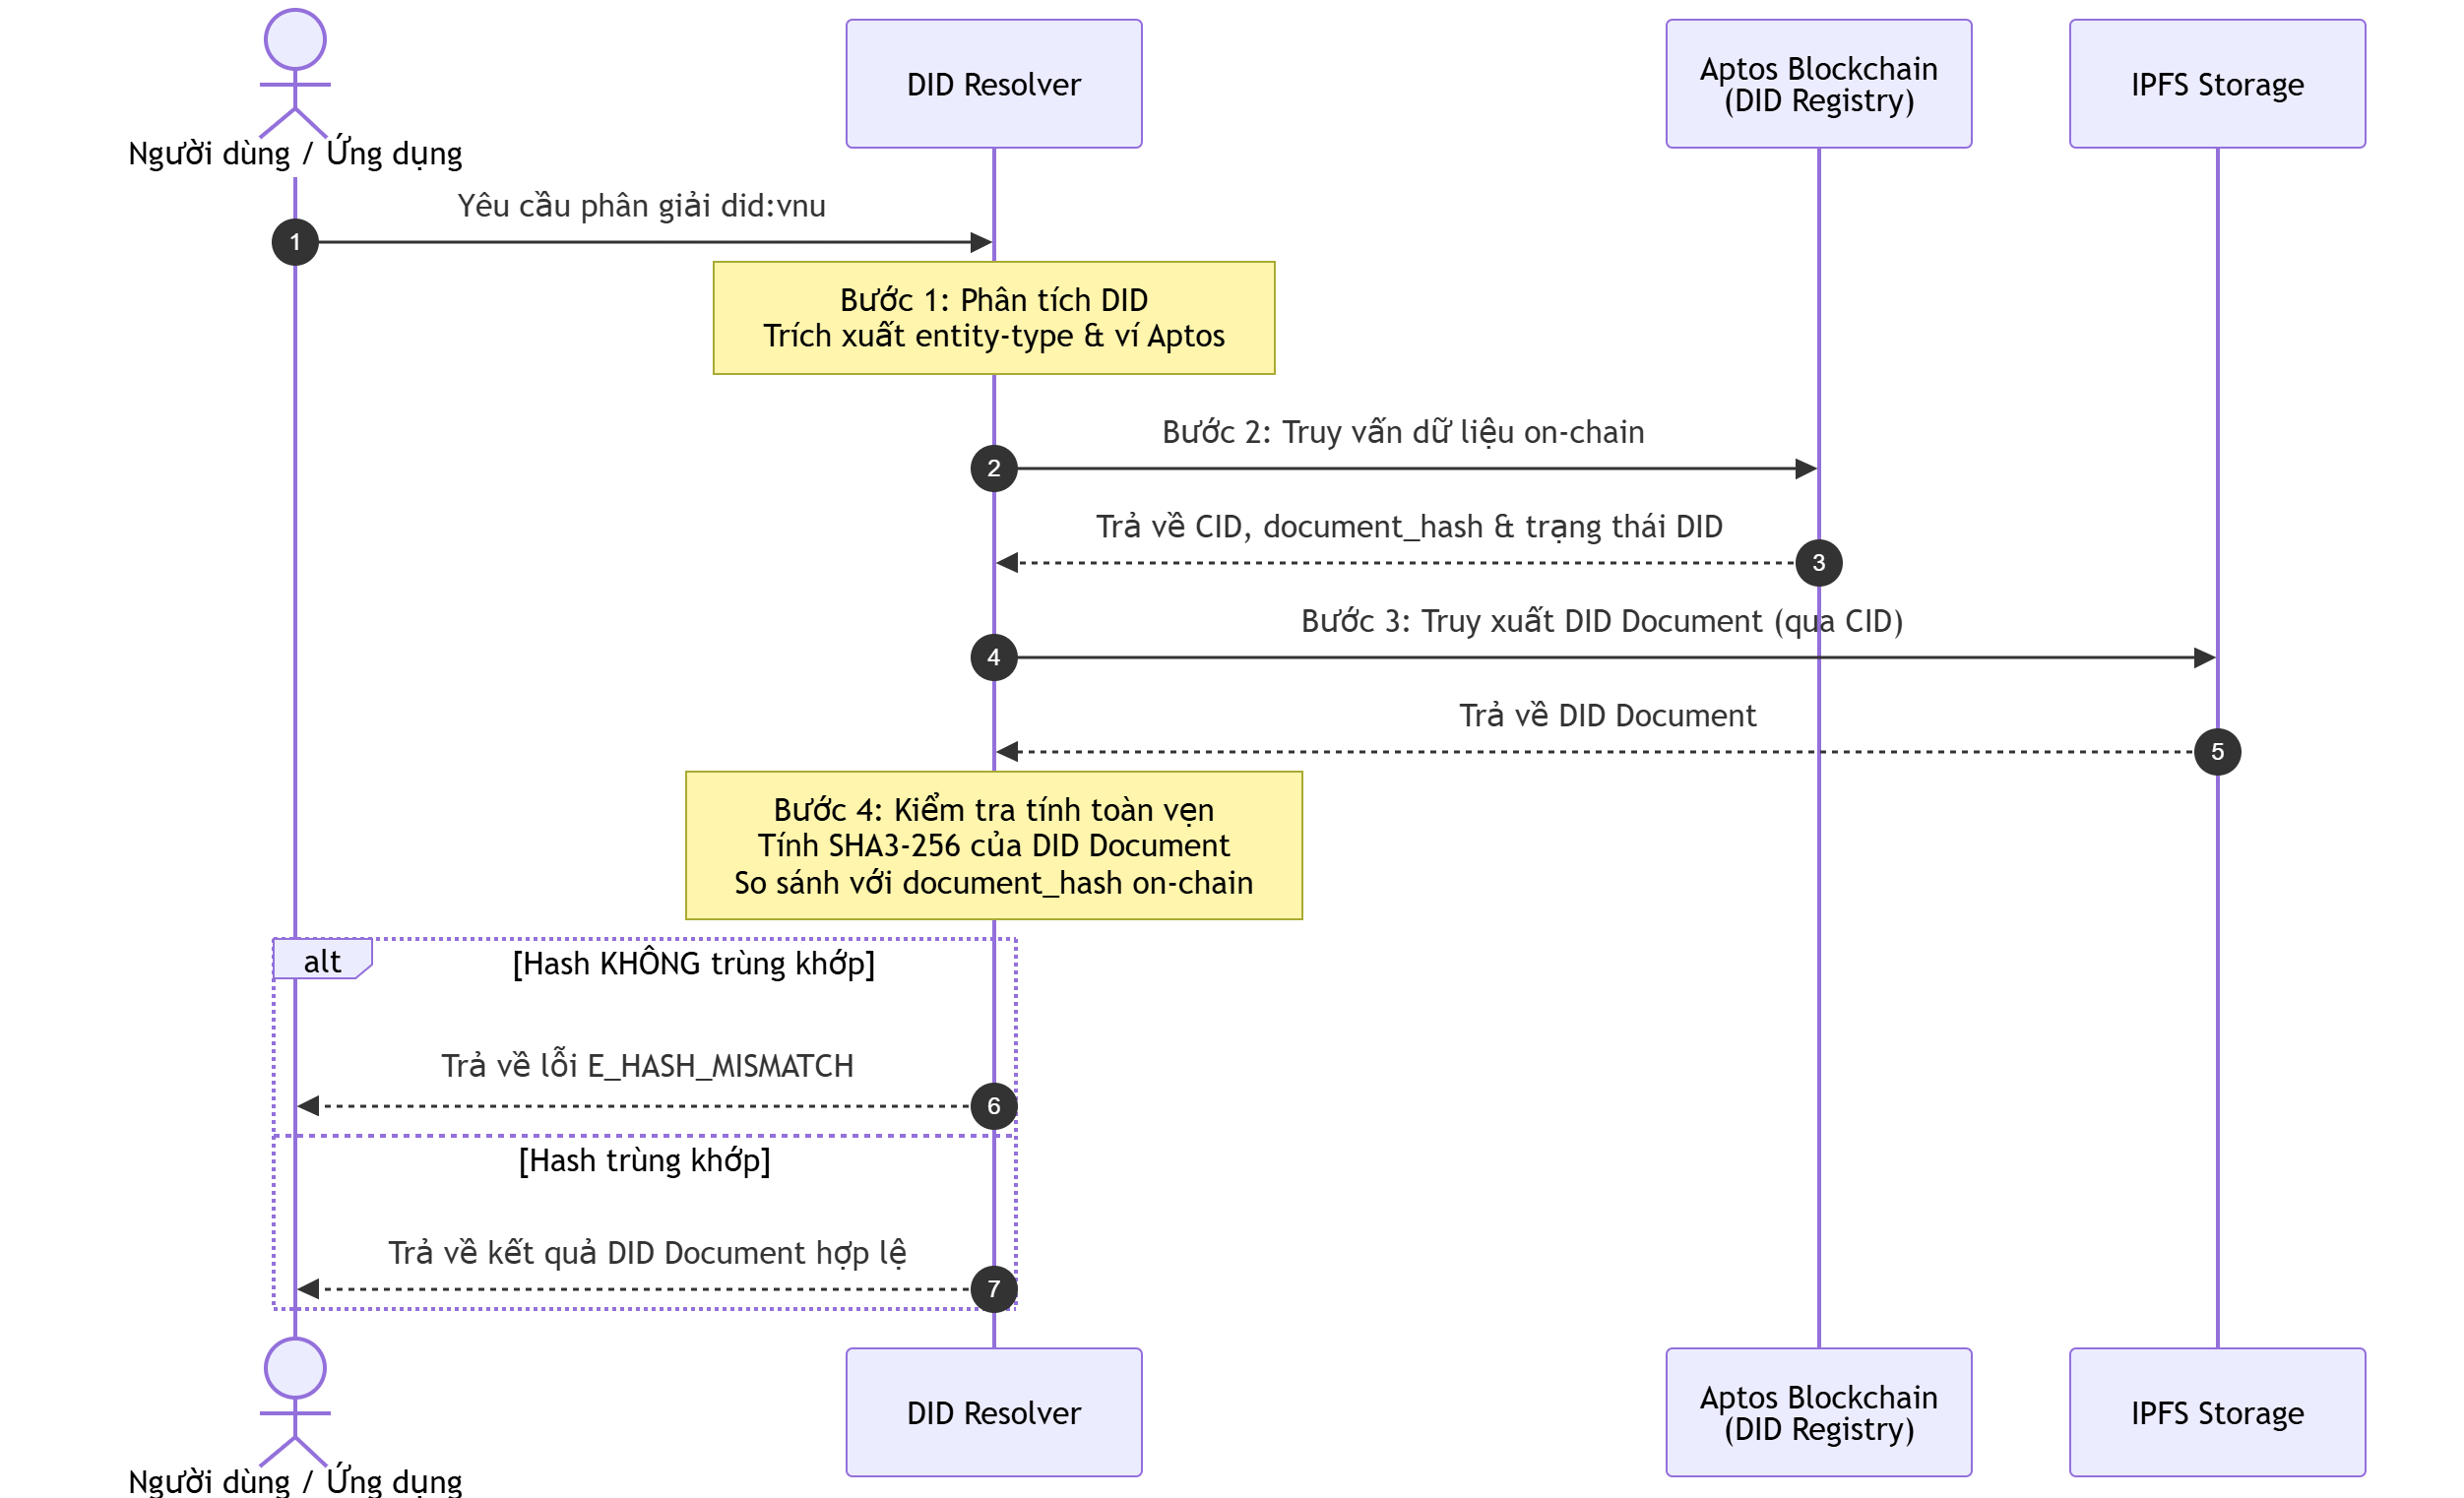
\includegraphics[width=0.9\textwidth]{images/did-resolution.png}
    \caption{Quy trình phân giải định danh trong phương thức \texttt{did:vnu}}
    \label{fig:did-resolution}
\end{figure}

Bước thứ tư là điểm phân biệt thiết kế này với các triển khai chỉ đọc tài liệu từ lớp lưu trữ mà không kiểm tra lại. Về lý thuyết, cơ chế định địa chỉ theo nội dung đã bảo đảm rằng nội dung không thể thay đổi mà giữ nguyên định danh. Trên thực tế, giữa bên xác minh và lớp lưu trữ còn có các cổng truy cập trung gian, và kết quả nhận về phụ thuộc vào cổng đó hoạt động đúng. Việc tính lại giá trị băm và đối chiếu với giá trị đã neo trên chuỗi loại bỏ sự phụ thuộc này: dù cổng nào trả về dữ liệu, bên xác minh vẫn phát hiện được sự không nhất quán.

\textbf{Về cơ chế xoay vòng khóa.} Khi một thực thể cần thay cặp khóa --- do nghi ngờ lộ khóa hoặc theo chu kỳ định kỳ --- thực thể đó dựng DID Document mới chứa khóa công khai mới, ghim lên lớp lưu trữ ngoài chuỗi để nhận định danh nội dung mới, rồi gọi thao tác cập nhật trên hợp đồng bằng chữ ký của khóa \emph{hiện tại}, qua đó chứng minh quyền kiểm soát định danh. Hợp đồng cập nhật định danh nội dung, giá trị băm và tăng số phiên bản. Các phiên bản trước vẫn được giữ, nhờ đó các chứng thực đã phát hành bằng khóa cũ vẫn xác minh được --- đáp ứng đúng yêu cầu đã nêu ở Mục 2.3.1 làm lý do thiết kế phương thức riêng. Thao tác cập nhật cũng nhận một tham số phiên bản kỳ vọng, nhằm phát hiện trường hợp hai cập nhật đồng thời ghi đè lên nhau.

\section{Quy trình xác minh}

\subsection{Bảy bước kiểm tra}

Quy trình xác minh được thiết kế theo nguyên tắc: mỗi bước kiểm tra một tính chất độc lập, và kết quả của từng bước được báo riêng. Cách này cho phép bên xác minh biết chính xác nguyên nhân thất bại --- điều mà Mục 2.8 xác định là một trong bốn khoảng trống của các hệ thống hiện có.

\begin{figure}[H]
    \centering
    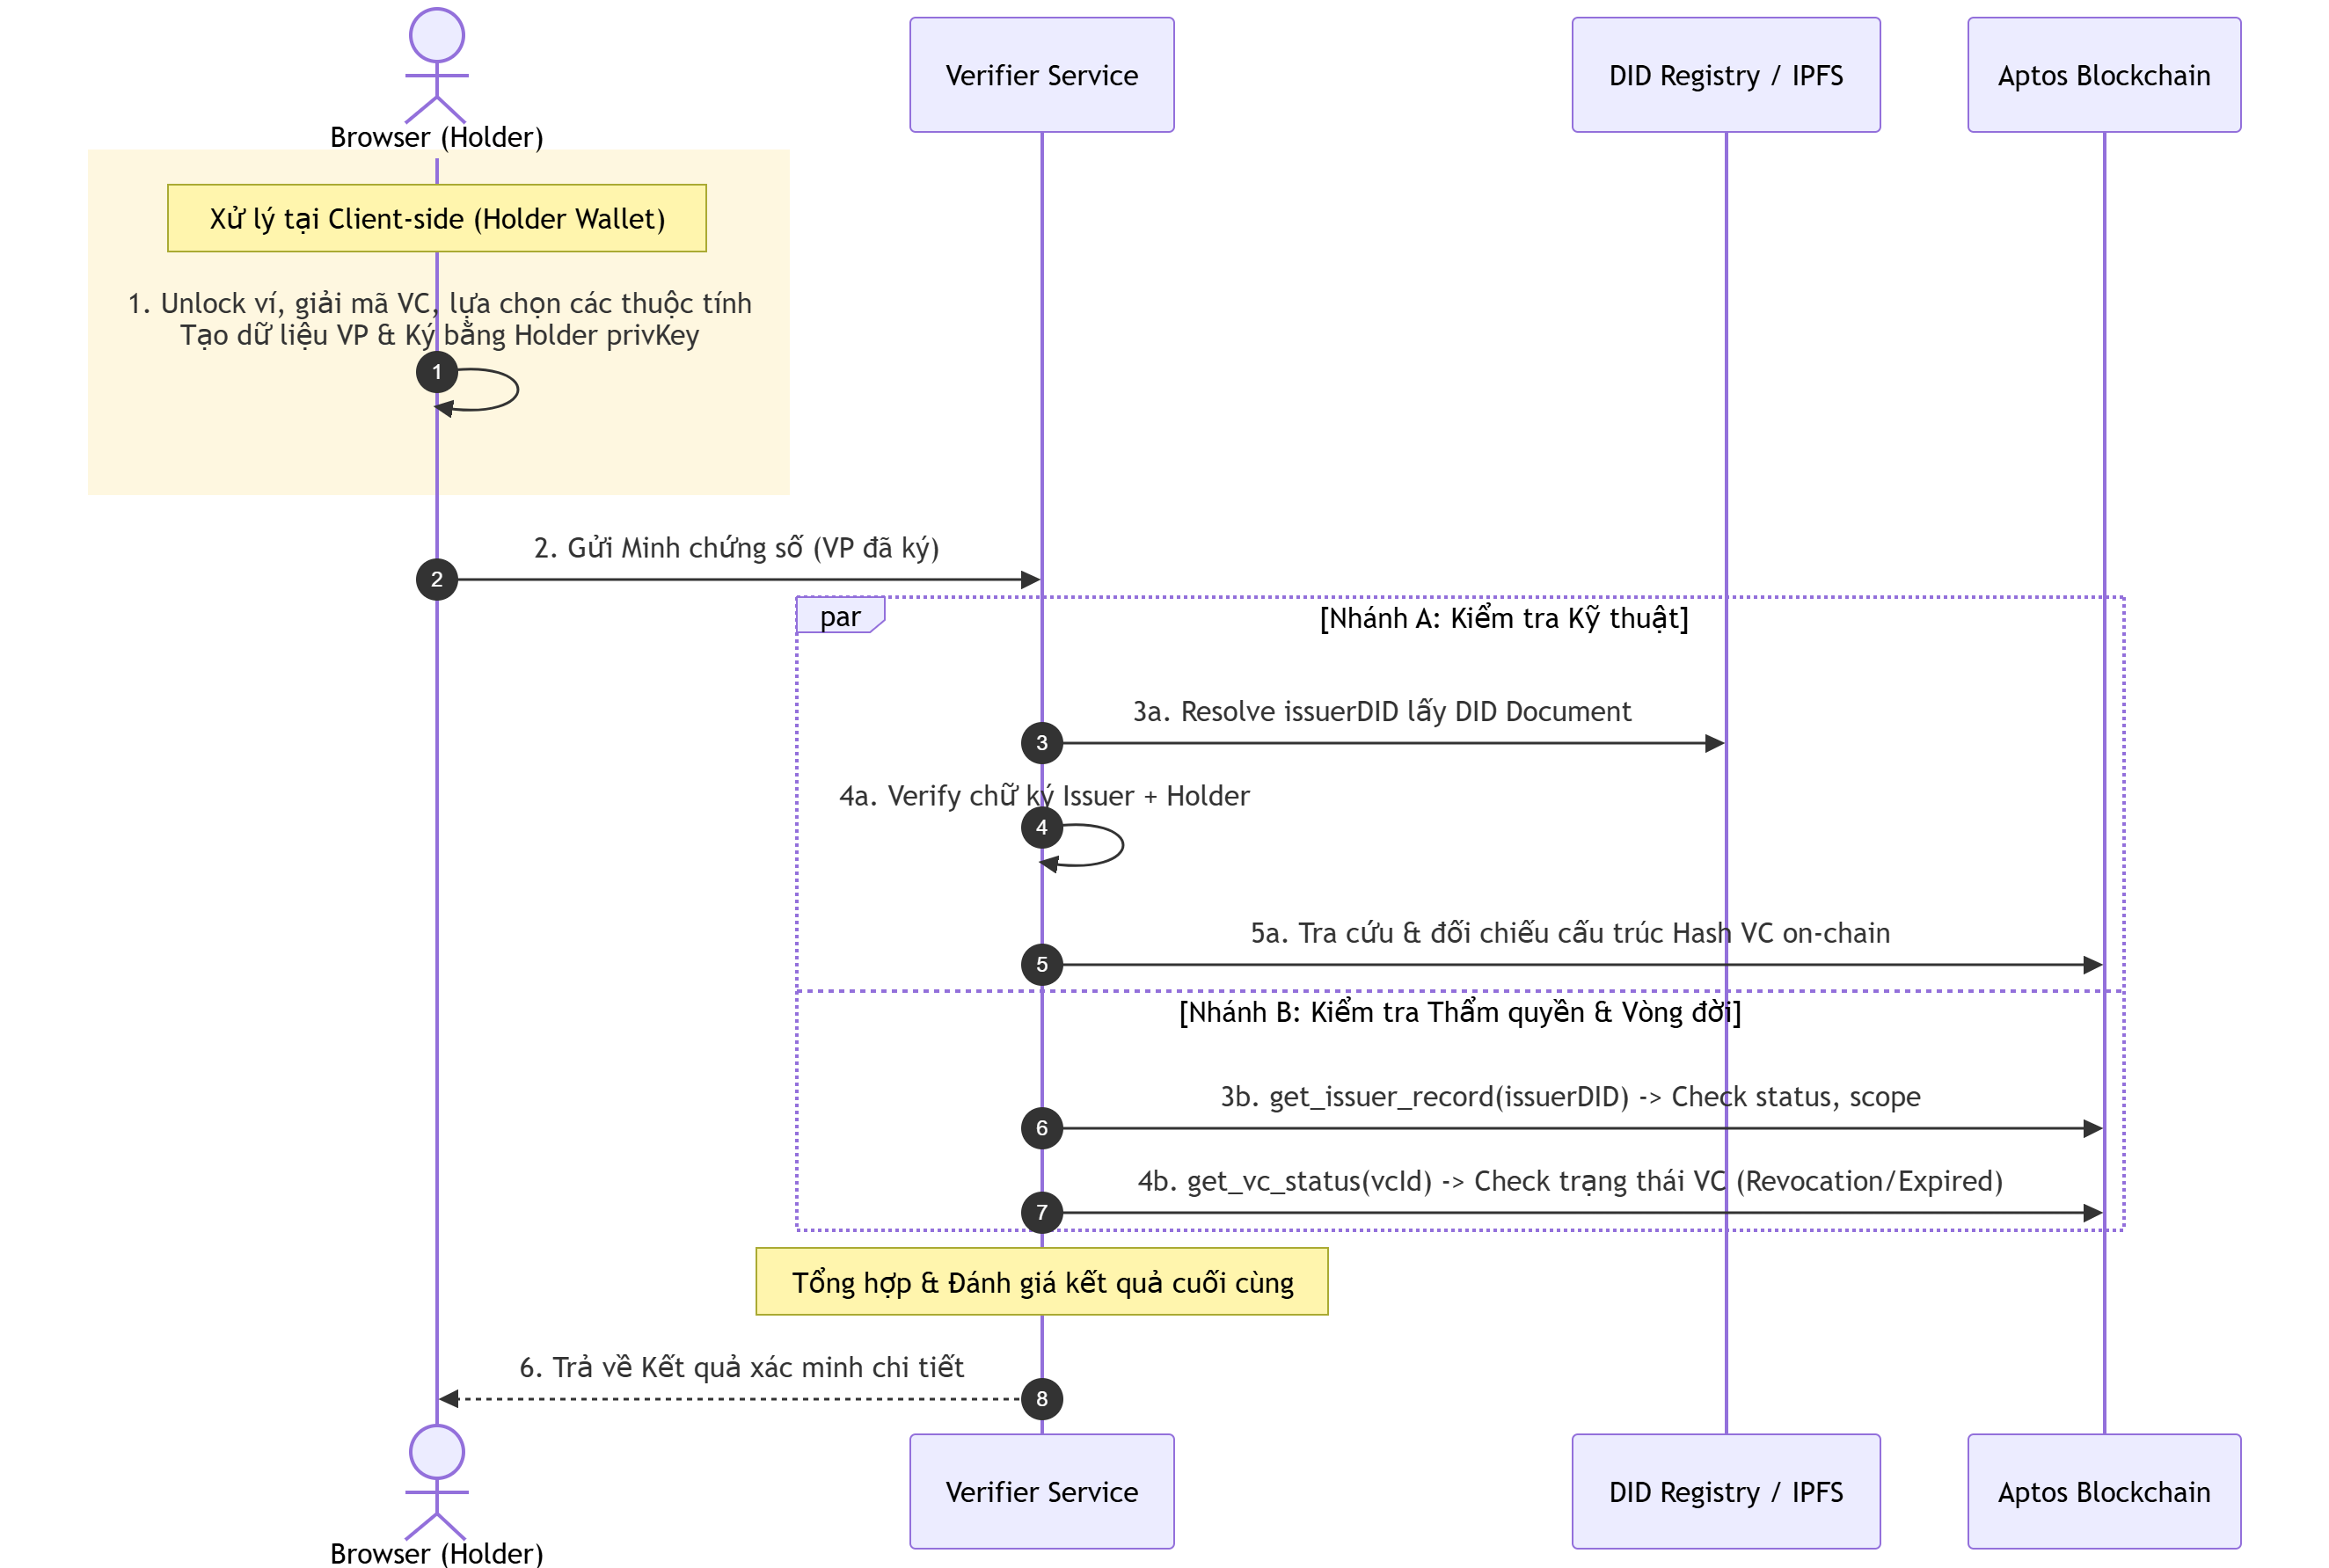
\includegraphics[width=1\textwidth]{images/seq_xac_minh_vp.png}
    \caption{Sơ đồ tuần tự quy trình trình bày và xác minh}
    \label{fig:seq_xac_minh_vp}
\end{figure}

Bảy bước, chia thành hai nhóm:

\noindent \textbf{Nhóm kỹ thuật --- tính toàn vẹn và quyền sở hữu:}

\begin{enumerate}
    \item \textbf{Truy xuất bản trình bày.} Tải nội dung bản trình bày từ lớp lưu trữ ngoài chuỗi theo định danh nội dung. Thất bại ở bước này nghĩa là dữ liệu không khả dụng, không phải dữ liệu không hợp lệ --- hai tình huống khác nhau cần được báo khác nhau.
    \item \textbf{Toàn vẹn bản trình bày.} Tính lại giá trị băm của nội dung nhận được và đối chiếu với giá trị đã ghi nhận.
    \item \textbf{Chữ ký của người trình bày.} Kiểm tra chữ ký trên bản trình bày bằng khóa công khai của chủ thể. Bước này xác lập rằng người trình bày đúng là chủ thể của chứng thực, không phải người đã lấy được một bản sao.
    \item \textbf{Trạng thái định danh của người trình bày.} Phân giải định danh của chủ thể và kiểm tra định danh đó còn hoạt động. Một định danh đã bị thu hồi --- chẳng hạn vì lộ khóa --- không được dùng để trình bày chứng thực.
\end{enumerate}

\noindent \textbf{Nhóm thẩm quyền và trạng thái:}

\begin{enumerate}
    \setcounter{enumi}{4}
    \item \textbf{Trạng thái hiệu lực của từng chứng thực.} Truy vấn trạng thái của từng chứng thực trong bản trình bày, bao gồm cả việc đánh giá thời điểm hết hạn.
    \item \textbf{Nội dung chứng thực khớp bản neo trên chuỗi.} Tính lại giá trị băm của nội dung chứng thực đang được trình bày và đối chiếu với giá trị băm đã neo trên chuỗi tại thời điểm cấp phát.
    \item \textbf{Thẩm quyền của bên phát hành.} Tra cứu trạng thái thẩm quyền của bên phát hành từng chứng thực trên chuỗi.
\end{enumerate}

Bước thứ sáu đáng được phân tích riêng, bởi nó là bước mà các hệ thống chỉ theo dõi trạng thái không có, và sự thiếu vắng của nó tạo ra một lỗ hổng cụ thể. Bước thứ năm trả lời câu hỏi {``}chứng thực này còn hiệu lực hay không{''}. Nó \emph{không} phát hiện được trường hợp nội dung chứng thực bị sửa sau khi cấp: nếu một bên nào đó sửa một trường trong nội dung --- chẳng hạn xếp loại hoặc điểm trung bình --- rồi ghim lại nội dung đã sửa, thì trạng thái của bản ghi trên chuỗi vẫn là {``}đang hiệu lực{''}, và cả bước thứ năm lẫn bước thứ bảy đều cho kết quả đạt. Phép kiểm duy nhất phát hiện được tình huống này là đối chiếu nội dung với giá trị băm đã neo.

Điều này không phải một khả năng lý thuyết. Mục 4.7 trình bày một kịch bản kiểm thử sửa nội dung trực tiếp trong chỉ mục rồi kiểm rằng bước toàn vẹn thất bại trong khi bước trạng thái vẫn đạt --- đúng để chứng minh rằng bước thứ sáu không dư thừa, và rằng một quy trình thiếu nó sẽ bỏ sót loại tấn công này.

\subsection{Ma trận kết quả xác minh}

Kết quả cuối cùng của quy trình là hợp lệ khi và chỉ khi cả bảy bước đều đạt. Tuy nhiên báo cáo xác minh không chỉ trả về một kết luận nhị phân mà trả về trạng thái của từng bước kèm chi tiết, bởi ba loại thất bại dưới đây có ý nghĩa xử lý hoàn toàn khác nhau.

\begin{longtable}{|p{2.3cm}|p{2.6cm}|p{2.2cm}|p{6.2cm}|}
\caption{Ma trận kết quả xác minh và ý nghĩa của từng loại thất bại}
\label{tab:verification-matrix} \\

\hline
\textbf{Nhóm kỹ thuật} & \textbf{Nhóm thẩm quyền} & \textbf{Kết quả} & \textbf{Ý nghĩa đối với bên xác minh} \\
\hline
\endfirsthead

\hline
\textbf{Nhóm kỹ thuật} & \textbf{Nhóm thẩm quyền} & \textbf{Kết quả} & \textbf{Ý nghĩa đối với bên xác minh} \\
\hline
\endhead

\hline
\endfoot

\hline
\endlastfoot

Đạt & Đạt & Hợp lệ
& Văn bằng hợp lệ cả về nội dung lẫn thẩm quyền cấp phát. Có thể chấp nhận.
\\ \hline

Không đạt & Đạt & Từ chối
& Nội dung bị sửa, chữ ký sai, hoặc bản trình bày do thực thể khác ký. Đây là dấu hiệu của gian lận chủ động và cần được báo cáo.
\\ \hline

Đạt & Không đạt & Từ chối
& Nội dung nguyên vẹn nhưng chứng thực đã bị thu hồi, đã hết hạn, hoặc bên phát hành không còn thẩm quyền. Báo cáo chỉ rõ nguyên nhân nào trong ba nguyên nhân này.
\\ \hline

Không đạt & Không đạt & Từ chối
& Báo cáo liệt kê đầy đủ các bước không đạt thay vì dừng ở bước đầu tiên, để bên xác minh thấy toàn bộ vấn đề.
\\ \hline

\end{longtable}


Sự phân biệt này có giá trị thực tiễn trực tiếp. Khi nội dung bị sửa, bên xác minh đang đối mặt với một hành vi gian lận chủ động và cần báo cáo. Khi chứng thực đã bị thu hồi, văn bằng đã từng hợp lệ nhưng không còn --- một tình huống hành chính bình thường. Khi bên phát hành mất thẩm quyền, bản thân chứng thực có thể vẫn đúng về nội dung, nhưng giá trị thể chế của nó cần được xem xét lại. Một kết quả {``}không hợp lệ{''} chung không cho phép phân biệt ba tình huống này.

\section{Mô hình đe dọa và các rào chắn}

Mục này kiểm tra lại tính đầy đủ của thiết kế bằng cách đi từ phía kẻ tấn công: liệt kê các hành vi mà một bên có ý đồ xấu có thể thực hiện, và xác định rào chắn nào ngăn mỗi hành vi đó.

\subsection{Giả định về năng lực của kẻ tấn công}

Mô hình đe dọa giả định kẻ tấn công có các năng lực sau: gửi được yêu cầu bất kỳ tới tầng dịch vụ, bao gồm yêu cầu có dữ liệu được dựng cố ý; đọc được mọi dữ liệu công khai trên chuỗi và trên lớp lưu trữ ngoài chuỗi khi biết định danh nội dung; và kiểm soát một tài khoản hợp lệ của chính mình, kèm khóa riêng tương ứng.

Mô hình \emph{không} giả định kẻ tấn công: chiếm được khóa riêng của người dùng khác; thực thi được mã trong trình duyệt của người dùng khác; hay làm sai lệch được trạng thái của chuỗi. Ba năng lực này nằm ngoài phạm vi phòng vệ của thiết kế, và hệ quả của chúng được thảo luận ở Mục 5.3.

Trong ba năng lực nằm ngoài phạm vi, một trường hợp cần được nêu riêng vì hệ quả của nó rộng hơn các trường hợp còn lại: \textbf{khóa riêng của một bên phát hành bị lộ}. Thiết kế hiện tại cho phép mỗi bên phát hành ký bằng một khóa duy nhất, nên kẻ chiếm được khóa đó cấp được chứng thực hợp lệ trong toàn bộ phạm vi thẩm quyền của đơn vị, cho tới khi thẩm quyền bị thu hồi. Đây là một đặc điểm chung của các hệ thống chứng nhận văn bằng dựa trên chữ ký đơn \cite{Saramago2021}, và nó không được giảm nhẹ bởi cơ chế hai bước ở Mục 3.4.4 --- cơ chế đó chỉ áp dụng cho việc chuyển quyền quản trị gốc.

Ba biện pháp giảm nhẹ \emph{một phần} có trong thiết kế: thẩm quyền có thời hạn nên thiệt hại bị chặn trên về thời gian; thẩm quyền có phạm vi nên thiệt hại bị chặn trên về loại văn bằng; và mọi chứng thực đã cấp đều thu hồi được, kể cả sau khi thẩm quyền của đơn vị đã bị thu hồi, theo nguyên tắc ở Mục 3.4.5. Biện pháp xử lý triệt để --- yêu cầu nhiều chữ ký hoặc chữ ký ngưỡng cho thao tác cấp phát --- nằm ngoài phạm vi bản thử nghiệm và được nêu tại Mục 5.4.

Một giới hạn về phương pháp cần được nêu ngay tại đây, trước khi trình bày kết quả. Mô hình đe dọa dưới đây do chính nghiên cứu định nghĩa, nên việc hệ thống chặn được toàn bộ các hành vi trong mô hình là \textbf{điều kiện cần chứ không phải điều kiện đủ} để kết luận về mức an toàn. Một mô hình tự định nghĩa luôn có nguy cơ bỏ sót đúng những hành vi mà người thiết kế không nghĩ tới --- và đó cũng là những hành vi nguy hiểm nhất. Để giảm nguy cơ này, các hành vi được liệt kê không xuất phát từ việc suy luận trên thiết kế mà từ ba nguồn độc lập hơn: các lỗi thật phát hiện trong đợt rà soát hợp đồng (Mục 4.3.5), các lỗi thật phát hiện khi đối chiếu hai cài đặt của tầng chỉ mục (Mục 4.4.1), và các loại tấn công được nêu trong tài liệu về định danh tự chủ \cite{Krul2024, Ambati2026}. Dù vậy, giới hạn vẫn còn và được thảo luận tại Mục 4.11.

\subsection{Các hành vi tấn công và rào chắn tương ứng}

\begin{longtable}{|c|p{3.6cm}|p{5.3cm}|p{3.4cm}|}
\caption{Mô hình đe dọa và rào chắn tương ứng}
\label{tab:threat-model} \\

\hline
\textbf{Mã} & \textbf{Hành vi tấn công} & \textbf{Rào chắn} & \textbf{Vị trí rào chắn} \\
\hline
\endfirsthead

\hline
\textbf{Mã} & \textbf{Hành vi tấn công} & \textbf{Rào chắn} & \textbf{Vị trí rào chắn} \\
\hline
\endhead

\hline
\endfoot

\hline
\endlastfoot

T1 & Tự khai là bên phát hành rồi cấp văn bằng
& Hợp đồng kiểm thẩm quyền trước khi ghi bản ghi; địa chỉ không có bản ghi thẩm quyền đang hoạt động thì thao tác thất bại
& Hợp đồng
\\ \hline

T2 & Cấp loại văn bằng ngoài phạm vi được phép
& Phép giao bit giữa loại văn bằng và mặt nạ phạm vi; kết quả bằng không thì từ chối
& Hợp đồng
\\ \hline

T3 & Tiếp tục cấp văn bằng sau khi thẩm quyền đã hết hạn
& Hợp đồng đối chiếu thời hạn ủy quyền với dấu thời gian của chuỗi
& Hợp đồng
\\ \hline

T4 & Khai báo mã giao dịch không tồn tại để tạo bản ghi về văn bằng không có trên chuỗi
& Bốn phép kiểm với nút đầy đủ trước khi ghi chỉ mục: giao dịch tồn tại; thành công; đúng hàm được gọi; đúng người gửi
& Tầng dịch vụ
\\ \hline

T5 & Tái sử dụng một giao dịch thật của chính mình nhưng thuộc loại thao tác khác
& Phép kiểm thứ ba trong T4: so khớp tên hàm trong phần tải của giao dịch với hàm mong đợi của tuyến
& Tầng dịch vụ
\\ \hline

T6 & Tái sử dụng giao dịch của người khác
& Phép kiểm thứ tư trong T4: so khớp người gửi giao dịch với tài khoản đang thực hiện yêu cầu
& Tầng dịch vụ
\\ \hline

T7 & Sửa nội dung văn bằng sau khi cấp rồi ghim lại nội dung đã sửa
& Bước thứ sáu của quy trình xác minh: tính lại giá trị băm của nội dung và đối chiếu với giá trị đã neo trên chuỗi
& Quy trình xác minh
\\ \hline

T8 & Trình bày một chứng thực của người khác đã lấy được bản sao
& Bước thứ ba của quy trình xác minh: chữ ký của người trình bày phải khớp khóa công khai của chủ thể ghi trong chứng thực
& Quy trình xác minh
\\ \hline

T9 & Khai báo giá trị băm sai để nội dung không khớp vẫn được chấp nhận
& Giá trị băm do máy khách khai báo đều được tính lại từ chính nội dung để đối chiếu trước khi ghi
& Tầng dịch vụ
\\ \hline

T10 & Mạo danh người khác khi đăng nhập bằng cách gửi lại chữ ký đã thu được
& Đăng nhập theo cơ chế thách thức -- đáp ứng với số dùng một lần có thời hạn; số đã dùng bị đánh dấu và không nhận lại
& Tầng dịch vụ
\\ \hline

T11 & Lợi dụng vai trò ghi trong phiên đăng nhập để thực hiện thao tác vượt quyền
& Các tuyến ghi có hệ quả trên chuỗi kiểm quyền trực tiếp trên chuỗi, không dựa vào vai trò trong phiên
& Tầng dịch vụ và hợp đồng
\\ \hline

T12 & Gán quyền gốc cho một địa chỉ không ai kiểm soát, qua đó làm mất năng lực quản trị
& Chuyển quyền gốc gồm hai bước; quyền chỉ chuyển sau khi người được đề cử tự ký để tiếp nhận
& Hợp đồng
\\ \hline

T13 & Đơn vị tự đình chỉ chứng thực rồi tự kích hoạt lại để xóa dấu vết
& Thao tác kích hoạt lại chỉ thuộc quản trị viên, không thuộc bên phát hành
& Hợp đồng
\\ \hline

T14 & Đăng ký một chuỗi định danh đã thuộc về thực thể khác
& Hợp đồng kiểm tính duy nhất của chuỗi định danh; đăng ký lại cho cùng một địa chỉ chỉ được phép sau khi định danh cũ đã bị thu hồi
& Hợp đồng
\\ \hline

T15 & Khai thác cổng truy cập trung gian để trả về nội dung khác nội dung đã đăng ký
& Phân giải định danh tính lại giá trị băm của tài liệu nhận được và đối chiếu với giá trị đã neo, bất kể nội dung đến từ cổng nào
& Quy trình phân giải
\\ \hline

\end{longtable}


Hai nhận xét về bảng trên.

Thứ nhất, \textbf{rào chắn cho các hành vi nghiêm trọng nhất đều nằm trong hợp đồng, không nằm trong tầng dịch vụ}. Điều này có chủ đích. Một rào chắn đặt ở tầng dịch vụ chỉ hiệu lực khi kẻ tấn công buộc phải đi qua dịch vụ đó; nhưng vì chuỗi là công khai, kẻ tấn công có thể gọi trực tiếp hợp đồng và bỏ qua hoàn toàn tầng dịch vụ. Vì vậy mọi quy tắc phân quyền phải được thi hành ở nơi không thể bị bỏ qua.

Thứ hai, \textbf{hành vi khai báo một tham chiếu giao dịch không tồn tại là hành vi đáng chú ý nhất về mặt thiết kế}. Trong một kiến trúc mà cơ sở dữ liệu chỉ là chỉ mục, mỗi bản ghi chỉ mục đều mang một tham chiếu tới giao dịch trên chuỗi đã tạo ra nó. Nếu tầng dịch vụ ghi nhận tham chiếu nào mà máy khách khai báo, thì máy khách chỉ cần gửi một chuỗi thập lục phân bất kỳ là tạo được một bản ghi về một văn bằng không tồn tại trên chuỗi. Rào chắn là bốn phép kiểm với nút đầy đủ trước khi ghi: giao dịch tồn tại; giao dịch thành công; hàm được gọi đúng là hàm mong đợi; và người gửi giao dịch khớp với tài khoản đang thực hiện yêu cầu. Thiếu phép kiểm thứ ba, kẻ tấn công có thể tái sử dụng một giao dịch thật của mình nhưng thuộc loại khác; thiếu phép kiểm thứ tư, họ có thể tái sử dụng giao dịch của người khác.

\section{Các đánh đổi trong quyết định thiết kế}

Mỗi quyết định kiến trúc đều kèm đánh đổi. Các đánh đổi dưới đây được ghi nhận tường minh --- không phải như hạn chế cần tránh nói tới, mà như kết quả của việc lựa chọn có chủ đích giữa những thuộc tính không thể đạt đồng thời.

\begin{longtable}{|p{2.9cm}|p{3.6cm}|p{3.6cm}|p{3.8cm}|}

\caption{Các đánh đổi trong quyết định thiết kế hệ thống
\label{tab:design-tradeoff}} \\

\hline
\textbf{Quyết định} &
\textbf{Thuộc tính thu được} &
\textbf{Thuộc tính phải hy sinh} &
\textbf{Cơ sở của lựa chọn} \\
\hline
\endfirsthead

\hline
\textbf{Quyết định} &
\textbf{Thuộc tính thu được} &
\textbf{Thuộc tính phải hy sinh} &
\textbf{Cơ sở của lựa chọn} \\
\hline
\endhead

\hline
\endfoot

\hline
\endlastfoot

Sổ đăng ký tin cậy trên chuỗi công khai thay cho cơ sở dữ liệu
&
Bên xác minh đọc được trạng thái thẩm quyền trực tiếp, không cần quan hệ trước với tổ chức nào; lịch sử quản trị không thể sửa
&
Chi phí giao dịch cho mỗi thao tác quản trị; trạng thái thẩm quyền trở thành thông tin công khai
&
Nếu sổ đăng ký là cơ sở dữ liệu thì bên xác minh lại phải tin tổ chức vận hành nó --- tức chỉ di chuyển sự phụ thuộc chứ không loại bỏ
\\ \hline

Một nguồn niềm tin gốc duy nhất
&
Mô hình quản trị đơn giản, trách nhiệm rõ ràng, phù hợp phạm vi kiểm chứng khái niệm
&
Tồn tại một điểm tập trung quyền lực quản trị
&
Phản ánh đúng cấu trúc thể chế hiện có của ĐHQGHN; kiến trúc phân lớp cho phép chuyển sang mô hình liên hợp mà không thay đổi ba lớp dưới
\\ \hline

Ví không lưu ký
&
Chủ thể là bên duy nhất ký được bản trình bày của mình, nhờ đó bước kiểm tra chữ ký của người trình bày có giá trị thật
&
Trải nghiệm phức tạp hơn; mất cụm từ khôi phục là mất quyền truy cập, không có cơ chế đặt lại
&
Mô hình lưu ký làm thay đổi tính chất an toàn mà hệ thống cung cấp, không chỉ làm giảm tính tự chủ về nguyên tắc
\\ \hline

Tách dữ liệu trên chuỗi và ngoài chuỗi
&
Chi phí lưu trữ thấp; không có dữ liệu cá nhân trên hạ tầng không thể xóa
&
Phụ thuộc vào tính khả dụng dài hạn của lớp lưu trữ ngoài chuỗi và cơ chế ghim
&
Ghi dữ liệu cá nhân lên hạ tầng bất biến khiến không thể thực hiện quyền của chủ thể dữ liệu theo quy định pháp luật
\\ \hline

Trạng thái theo từng bản ghi thay cho danh sách bit
&
Truy vấn trạng thái tức thời; thống nhất hạ tầng của ba sổ đăng ký trên cùng một lớp
&
Mỗi lần thu hồi là một giao dịch riêng; mỗi lần tra cứu để lại dấu vết về chứng thực được kiểm tra
&
Đơn giản hóa vận hành ở quy mô thử nghiệm; đây là điểm cần chuyển đổi khi mở rộng, và chỉ ảnh hưởng tới lớp chứng thực
\\ \hline

Chuẩn hóa JSON thay cho chuẩn hóa tập dữ liệu RDF
&
Triển khai được bằng mã ngắn, đồng nhất được giữa nhiều ngôn ngữ, dễ kiểm chứng tính tất định
&
Chỉ bảo đảm tương đương ở mức cú pháp; bên xác minh ngoài hệ thống cần mã kiểm tra riêng
&
Tương đương ngữ nghĩa của RDF yêu cầu bên xác minh triển khai toàn bộ phép xử lý JSON-LD, chi phí không tương xứng ở phạm vi hiện tại
\\ \hline

Giao diện dịch vụ theo kiểu REST thay cho giao thức truyền thông điệp giữa các tác nhân
&
Giảm đáng kể độ phức tạp triển khai và tích hợp
&
Khả năng tương tác giữa các hệ sinh thái thấp hơn kiến trúc tham chiếu đầy đủ
&
Phù hợp mục tiêu kiểm chứng mô hình quản trị; việc bổ sung giao thức truyền thông điệp không làm thay đổi kết luận về khung quản trị
\\ \hline

Giới hạn chuỗi ủy quyền ở hai cấp
&
Trách nhiệm luôn truy vết được tới một đơn vị cụ thể
&
Không biểu diễn được cấu trúc tổ chức sâu hơn hai cấp
&
Chuỗi ủy quyền sâu không giới hạn khiến việc truy vết trách nhiệm trở nên bất khả thi, trong khi lợi ích không rõ ràng
\\ \hline

\end{longtable}


Hai đánh đổi có ảnh hưởng lớn nhất cần được phân tích thêm.

\noindent \textbf{Ví không lưu ký.} Đây là đánh đổi tác động mạnh nhất tới trải nghiệm người dùng. Quyết định chọn mô hình không lưu ký xuất phát từ một quan sát ở Mục 2.3.4: trong mô hình lưu ký, bên vận hành có khả năng kỹ thuật để ký thay người dùng, nên toàn bộ lập luận về việc {``}chủ thể là bên duy nhất trình bày được chứng thực của mình{''} không còn thành lập. Nếu lập luận đó không thành lập, thì bước kiểm tra chữ ký của người trình bày trong quy trình xác minh mất ý nghĩa, và một trong ba thuộc tính tin cậy bị suy giảm. Nói cách khác, đây không phải một lựa chọn về nguyên tắc mà là một ràng buộc kỹ thuật: mô hình lưu ký làm thay đổi tính chất an toàn mà hệ thống cung cấp. Giá phải trả là người dùng gánh trách nhiệm bảo vệ khóa, và việc mất cụm từ khôi phục đồng nghĩa với mất quyền truy cập.

\noindent \textbf{Trạng thái theo từng bản ghi thay cho danh sách bit.} Như đã phân tích ở Mục 2.3.3, cơ chế danh sách bit của chuẩn W3C hiệu quả hơn về chi phí và cung cấp quyền riêng tư theo nhóm. Thiết kế này chọn cơ chế theo từng bản ghi vì nó cho phép truy vấn trạng thái tức thời và thống nhất hạ tầng quản lý định danh, thẩm quyền và trạng thái chứng thực trên cùng một lớp, giảm số thành phần cần vận hành. Hai cái giá phải trả là rõ ràng: mỗi lần thu hồi là một giao dịch riêng, nên chi phí tăng tuyến tính theo số lần thu hồi; và mỗi lần tra cứu để lại dấu vết về việc chứng thực nào đang được kiểm tra. Ở quy mô thử nghiệm, cả hai đều trong mức chấp nhận được; ở quy mô triển khai thật, đây là điểm cần chuyển đổi, và việc chuyển đổi khả thi vì nó chỉ ảnh hưởng tới lớp chứng thực.

\section{Đối chiếu với các kiến trúc tham chiếu}

\subsection{Những gì được kế thừa}

Kiến trúc đề xuất không được xây dựng từ đầu mà kế thừa có chọn lọc từ các mô hình đã phân tích ở Mục 2.7.

Từ Trust over IP \cite{ToIP_Stack2022}, nghiên cứu kế thừa tư duy phân lớp và --- quan trọng hơn --- quan điểm rằng quản trị phải được xem xét như một chiều kiến trúc độc lập ngay từ đầu, không phải một thành phần bổ sung sau cùng. Các thành phần phức tạp hơn của kiến trúc tham chiếu, cụ thể là giao thức truyền thông điệp giữa các tác nhân \cite{DIDComm2021} và kiến trúc dựa trên tác nhân, không được sử dụng nhằm giảm độ phức tạp triển khai trong phạm vi kiểm chứng khái niệm.

Từ mô hình niềm tin của EBSI \cite{EBSI_TrustModel}, nghiên cứu kế thừa hai nguyên tắc đã nêu ở Mục 2.7.2: hạ tầng ghi nhận các quyết định về niềm tin nhưng không tạo ra chúng, và mỗi bên xác minh tự quyết định họ chấp nhận gốc niềm tin nào. Nghiên cứu cũng kế thừa ý tưởng biểu diễn bản thân quan hệ ủy quyền thành một chứng thực có thể xác minh, thay vì chỉ một cờ trạng thái.

Điểm khác biệt cơ bản so với EBSI là nơi lưu trữ sổ đăng ký tin cậy. Thay vì một hạ tầng do một tổ chức vận hành, sổ đăng ký trong mô hình đề xuất là trạng thái của một hợp đồng trên chuỗi công khai, nên trạng thái thẩm quyền trở thành dữ liệu mà bất kỳ bên nào cũng đọc được trực tiếp. Điều này xử lý đúng khoảng trống thứ hai đã nêu ở Mục 2.8: giải quyết tầng niềm tin thể chế bằng cách tập trung hóa chỉ di chuyển vấn đề chứ không loại bỏ nó.

\subsection{So sánh ở mức thiết kế}

% Sáu cột ở cỡ chữ thường thì tràn lề phải ~20pt và chữ bị giãn rất xấu.
% Thu nhỏ cỡ chữ, giảm đệm cột và canh trái các ô thay vì bỏ bớt cột.
\begingroup
\footnotesize
\setlength{\tabcolsep}{3pt}
\begin{longtable}{|>{\raggedright\arraybackslash}p{2.8cm}|>{\raggedright\arraybackslash}p{2.4cm}|>{\raggedright\arraybackslash}p{2.5cm}|>{\raggedright\arraybackslash}p{2.3cm}|>{\raggedright\arraybackslash}p{2.3cm}|>{\raggedright\arraybackslash}p{2.3cm}|}
\caption{So sánh mô hình đề xuất với các hệ thống và kiến trúc tham chiếu}
\label{tab:system-comparison} \\

\hline
\textbf{Tiêu chí} & \textbf{Blockcerts} & \textbf{EDC / EBSI} & \textbf{Open Badges 3.0} & \textbf{Trust over IP} & \textbf{Mô hình đề xuất} \\
\hline
\endfirsthead

\hline
\textbf{Tiêu chí} & \textbf{Blockcerts} & \textbf{EDC / EBSI} & \textbf{Open Badges 3.0} & \textbf{Trust over IP} & \textbf{Mô hình đề xuất} \\
\hline
\endhead

\hline
\endfoot

\hline
\endlastfoot

Xác minh độc lập với bên phát hành
& Có
& Phụ thuộc hạ tầng khu vực
& Có
& Theo thiết kế
& Có
\\ \hline

Sổ đăng ký thẩm quyền
& Không có
& Có, do tổ chức vận hành
& Không có
& Mô tả khái niệm
& Có, là trạng thái hợp đồng trên chuỗi công khai
\\ \hline

Biểu diễn phạm vi cấp phát
& Không
& Theo lĩnh vực và địa bàn
& Không
& Mô tả khái niệm
& Mặt nạ bit theo loại văn bằng
\\ \hline

Thời hạn ủy quyền
& Không
& Theo chu kỳ kiểm định
& Không
& Mô tả khái niệm
& Trường thời hạn trong bản ghi, hợp đồng tự đối chiếu
\\ \hline

Ủy quyền nhiều cấp
& Không
& Có, qua tổ chức kiểm định
& Không
& Hoãn ở đặc tả truy vấn v2.0
& Có, với ba ràng buộc thi hành bởi hợp đồng
\\ \hline

Thu hồi thẩm quyền
& Không
& Có
& Không
& Mô tả khái niệm
& Có, trạng thái cập nhật trên chuỗi
\\ \hline

Cơ chế thu hồi chứng thực
& Danh sách do bên phát hành tự giữ
& Tập trung
& Tùy triển khai
& Không quy định
& Trạng thái theo từng bản ghi trên chuỗi
\\ \hline

Đối chiếu nội dung với bản neo khi xác minh
& Có
& Có
& Tùy triển khai
& Không quy định
& Có, là một bước riêng trong quy trình
\\ \hline

Phân biệt loại thất bại khi xác minh
& Không
& Không rõ
& Không
& Không quy định
& Có, báo cáo theo từng bước
\\ \hline

Chủ thể kiểm soát khóa
& Một phần
& Không
& Tùy triển khai
& Theo thiết kế
& Ví không lưu ký
\\ \hline

Tuân thủ chuẩn W3C DID / VC
& Một phần
& Một phần
& Có ở lớp chứng thực
& Tham chiếu chuẩn
& Tuân thủ, trừ phép chuẩn hóa và cơ chế trạng thái
\\ \hline

Cơ sở pháp lý đi kèm
& Không
& Có, theo khung eIDAS
& Không
& Không
& Chưa có; hành lang pháp lý trong nước đã hình thành
\\ \hline

\end{longtable}
\endgroup


Các mô hình hiện có chưa cân bằng được đồng thời ba thuộc tính: quản trị thẩm quyền, mức độ phi tập trung, và khả năng liên thông theo chuẩn mở. Blockcerts và Open Badges hỗ trợ xác minh độc lập nhưng thiếu quản trị bên phát hành; hạ tầng châu Âu có quản trị đầy đủ nhưng phụ thuộc hạ tầng tập trung; Trust over IP mô tả cả ba nhưng dừng ở mức kiến trúc tham chiếu.

\subsection{So sánh với mô hình truyền thống và mô hình định danh tự chủ thuần túy}

\begin{longtable}{|p{3.1cm}|p{3.5cm}|p{3.5cm}|p{3.5cm}|}
\caption{So sánh mô hình truyền thống, mô hình định danh tự chủ thuần túy và mô hình đề xuất}
\label{tab:traditional-ssi-comparison} \\

\hline
\textbf{Tiêu chí} & \textbf{Mô hình truyền thống} & \textbf{Định danh tự chủ thuần túy} & \textbf{Mô hình đề xuất} \\
\hline
\endfirsthead

\hline
\textbf{Tiêu chí} & \textbf{Mô hình truyền thống} & \textbf{Định danh tự chủ thuần túy} & \textbf{Mô hình đề xuất} \\
\hline
\endhead

\hline
\endfoot

\hline
\endlastfoot

Nơi đặt niềm tin
& Tổ chức trung gian
& Bằng chứng mật mã
& Bằng chứng mật mã cho nội dung; trạng thái công khai trên chuỗi cho thẩm quyền
\\ \hline

Điều kiện để xác minh
& Bên cấp phát hợp tác và còn tồn tại
& Truy cập được hạ tầng công bố khóa
& Truy cập được chuỗi và lớp lưu trữ ngoài chuỗi
\\ \hline

Chi phí một lần xác minh
& Tỉ lệ với số lần xác minh
& Gần như không đổi
& Gần như không đổi
\\ \hline

Phát hiện nội dung bị sửa
& Có, nếu đối chiếu được sổ gốc
& Có, bằng chữ ký
& Có, bằng chữ ký và bằng đối chiếu với giá trị băm đã neo
\\ \hline

Trả lời câu hỏi về thẩm quyền cấp phát
& Có, nhưng theo quy trình hành chính
& \textbf{Không}
& Có, bằng truy vấn công khai trên chuỗi
\\ \hline

Phạm vi và thời hạn của thẩm quyền
& Có trên văn bản, không kiểm chứng tự động được
& Không biểu diễn
& Biểu diễn tường minh và được hợp đồng thi hành
\\ \hline

Liên thông định danh giữa các cơ sở
& Không: mỗi cơ sở một mã riêng
& Có
& Có
\\ \hline

Chủ thể kiểm soát dữ liệu
& Không
& Có
& Có
\\ \hline

Dấu vết của thao tác quản trị
& Lưu nội bộ, có thể sửa
& Không có khái niệm quản trị
& Bất biến, công khai
\\ \hline

Phụ thuộc hạ tầng kỹ thuật
& Thấp
& Trung bình
& Cao: cần chuỗi, lớp lưu trữ ngoài chuỗi và ví
\\ \hline

Gánh nặng cho người học
& Thấp
& Cao: tự quản lý khóa
& Cao: tự quản lý khóa
\\ \hline

\end{longtable}


Bảng trên làm rõ vị trí của đóng góp. So với mô hình truyền thống, thay đổi nằm ở việc chuyển niềm tin từ trung gian sang bằng chứng, qua đó loại bỏ sự phụ thuộc vào bên cấp phát tại thời điểm xác minh. So với một hệ thống định danh tự chủ thuần túy, thay đổi nằm ở việc bổ sung lớp trả lời câu hỏi về thẩm quyền --- câu hỏi mà mật mã học không thể trả lời, và là lý do một hệ thống định danh tự chủ đúng về mặt kỹ thuật vẫn chưa đủ cho bài toán văn bằng.

% Chương 4: Triển khai và đánh giá
\chapter{TRIỂN KHAI VÀ ĐÁNH GIÁ}

\section{Phạm vi và môi trường triển khai}

\subsection{Phạm vi triển khai}

Chương này trình bày việc hiện thực hóa kiến trúc và khung quản trị ở Chương 3 thành một hệ thống hoạt động, nhằm kiểm chứng ba điều: logic phân quyền được đặc tả ở Mục 3.4 có đúng đắn và có thực sự chặn được các hành vi vi phạm; quy trình xác minh ở Mục 3.6 có phát hiện được các kịch bản gian lận trong mô hình đe dọa ở Mục 3.7; và hệ thống có hiệu năng đủ để việc xác minh trở thành thao tác thường xuyên chứ không phải ngoại lệ.

Hệ thống mô phỏng mô hình liên trường của ĐHQGHN: cơ quan quản trị quản lý sổ đăng ký tin cậy, các trường thành viên đóng vai trò bên phát hành, sinh viên là chủ thể, và bên xác minh hoạt động hoàn toàn độc lập.

Những nội dung nằm ngoài phạm vi triển khai được nêu rõ để tránh suy luận quá mức từ kết quả: tích hợp với hệ thống quản lý đào tạo thực tế; liên hợp giữa nhiều miền quản trị; sử dụng mô-đun bảo mật phần cứng để lưu khóa của cơ quan quản trị; kiểm thử tải ở quy mô sản xuất; và triển khai trên mạng chính.

\subsection{Thành phần và phiên bản}

\begin{longtable}{|p{3.4cm}|p{2.9cm}|p{7.3cm}|}
\caption{Thành phần và phiên bản của hệ thống thử nghiệm}
\label{tab:system-environment}
\\
\hline
\textbf{Thành phần} & \textbf{Phiên bản} & \textbf{Vai trò trong hệ thống} \\
\hline
\endfirsthead

\hline
\textbf{Thành phần} & \textbf{Phiên bản} & \textbf{Vai trò trong hệ thống} \\
\hline
\endhead

\hline
\endfoot

\hline
\endlastfoot

Mạng thử nghiệm Move
& Mã chuỗi 250
& Nguồn sự thật: định danh, thẩm quyền, trạng thái chứng thực \\
\hline

Trình biên dịch Move
& Phiên bản 3.x
& Biên dịch và xuất bản ba mô-đun hợp đồng \\
\hline

Node.js
& 20 LTS trở lên
& Môi trường chạy cài đặt TypeScript của tầng chỉ mục và công cụ phát triển giao diện \\
\hline

TypeScript
& 5.7
& Cài đặt thứ nhất của tầng chỉ mục, biên dịch ở chế độ kiểm kiểu nghiêm ngặt \\
\hline

Express, \texttt{pg}, \texttt{zod}
& 4.21 / 8.13 / 3.24
& Khung dịch vụ HTTP, truy cập cơ sở dữ liệu, kiểm tra lược đồ thân yêu cầu \\
\hline

Go
& 1.23
& Cài đặt thứ hai của tầng chỉ mục, dùng thư viện HTTP chuẩn \\
\hline

\texttt{pgx}, \texttt{golang-jwt}, \texttt{x/crypto}
& 5.7 / 5.2 / 0.31
& Truy cập cơ sở dữ liệu, ký phiên, hàm băm SHA-3 \\
\hline

PostgreSQL
& 16
& Tầng chỉ mục dùng chung cho cả hai cài đặt, kèm nhật ký kiểm toán \\
\hline

React, Vite, Tailwind
& 18.3 / 6.0 / 3.4
& Giao diện theo vai trò, gói phát hành 405\,KB \\
\hline

\texttt{@noble/curves}, \texttt{@noble/hashes}
& 1.9 / 1.8
& Ký Ed25519 và băm SHA3-256 phía máy khách, thay cho bộ công cụ của nền tảng \\
\hline

\texttt{@scure/bip39}
& 1.6
& Sinh và kiểm tra cụm từ ghi nhớ để khôi phục ví trên thiết bị khác \\
\hline

Web Cryptography API
& Theo trình duyệt
& Dẫn xuất khóa PBKDF2 và mã hóa AES-256-GCM cho kho khóa cục bộ \\
\hline

Indexed Database API
& Theo trình duyệt
& Lưu bản mã của kho khóa trên thiết bị người dùng \\
\hline

Dịch vụ ghim IPFS
& Giao diện HTTP
& Lưu DID Document và nội dung chứng thực ngoài chuỗi; có chế độ mô phỏng dùng cơ sở dữ liệu dùng chung \\
\hline

\end{longtable}


Hai điểm trong bảng trên khác với một triển khai thông thường và cần giải thích.

Thứ nhất, \textbf{tầng chỉ mục được hiện thực hóa hai lần bằng hai ngôn ngữ khác nhau} --- một bản TypeScript và một bản Go --- cài đặt cùng một hợp đồng giao diện trên cùng một lược đồ cơ sở dữ liệu. Lý do và giá trị kiểm chứng của quyết định này được trình bày tại Mục 4.4.

Thứ hai, \textbf{giao diện không sử dụng bộ công cụ phát triển chính thức của nền tảng chuỗi}. Toàn bộ thao tác mật mã và thao tác chuỗi phía máy khách được thực hiện bằng các thư viện mật mã độc lập. Cơ sở của quyết định này và cách nó được kiểm chứng được trình bày tại Mục 4.5.3.

\subsection{Quản lý thông số chuỗi}

Hệ thống có ba thành phần cùng cần biết địa chỉ gói hợp đồng và các thông số chuỗi: hai cài đặt của tầng chỉ mục và giao diện. Trong giai đoạn đầu, các thông số này được khai riêng trong tệp cấu hình của từng thành phần. Cách làm đó tạo ra một lớp lỗi khó chẩn đoán: khi triển khai lại hợp đồng mà cập nhật sót một tệp, hai cài đặt của tầng chỉ mục sẽ nói chuyện với hai gói hợp đồng khác nhau, và không thành phần nào báo lỗi --- mỗi bên đều hoạt động bình thường với gói mà nó biết, chỉ có kết quả là không nhất quán.

Thiết kế hiện tại đặt toàn bộ thông số chuỗi vào một tệp duy nhất ở gốc dự án, và một tập lệnh đồng bộ đẩy giá trị sang cấu hình của ba thành phần. Tập lệnh triển khai hợp đồng tự cập nhật tệp này sau khi xuất bản gói rồi gọi tập lệnh đồng bộ. Đây là một ví dụ nhỏ nhưng tiêu biểu cho một nguyên tắc chung trong hệ thống phân tán: một giá trị cần nhất quán giữa nhiều thành phần thì phải có đúng một nguồn, bởi sự nhất quán được duy trì bằng quy trình thủ công sẽ thất bại sớm hơn dự kiến.

\section{Lựa chọn nền tảng}

\subsection{Nền tảng chuỗi}

Việc lựa chọn nền tảng chuỗi ảnh hưởng tới cơ chế quản trị, độ trễ xác minh và khả năng mở rộng. Ba hướng được xem xét.

\begin{longtable}{|p{3.3cm}|p{3.3cm}|p{3.3cm}|p{3.3cm}|}
\caption{So sánh ba hướng nền tảng chuỗi cho hệ thống văn bằng số}
\label{tab:blockchain-comparison} \\
\hline
\textbf{Tiêu chí} & \textbf{Chuỗi công khai hợp đồng chung} & \textbf{Chuỗi được cấp phép} & \textbf{Chuỗi công khai máy ảo Move} \\
\hline
\endfirsthead

\hline
\textbf{Tiêu chí} & \textbf{Chuỗi công khai hợp đồng chung} & \textbf{Chuỗi được cấp phép} & \textbf{Chuỗi công khai máy ảo Move} \\
\hline
\endhead

\hline
\endfoot

\hline
\endlastfoot

Ngôn ngữ hợp đồng
& Solidity
& Go, Java, JavaScript
& Move
\\ \hline

Mô hình lập trình
& Hướng tài khoản
& Hướng tài khoản
& Hướng tài nguyên, hệ thống kiểu ngăn nhân bản và hủy ngoài ý muốn
\\ \hline

Kiểm soát truy cập giữa các mô-đun
& Theo quy ước và bộ sửa đổi do lập trình viên viết
& Theo chính sách của mạng
& Cơ chế \texttt{friend} ở tầng ngôn ngữ
\\ \hline

Thời gian xác nhận
& Khoảng 12 giây
& Dưới 1 giây
& Dưới 1 giây, nhờ thực thi song song
\\ \hline

Đọc dữ liệu không cần cấp phép
& Có
& \textbf{Không}: bên ngoài tập thành viên phải đi qua một cổng dịch vụ
& Có
\\ \hline

Chi phí ở giai đoạn thử nghiệm
& Cao và biến động theo thị trường
& Cần vận hành nút xác thực riêng
& Thấp trên mạng thử nghiệm
\\ \hline

Phù hợp cho kiểm chứng xác minh độc lập
& Có
& Không: không kiểm chứng được tính chất {``}không cần thỏa thuận trước{''}
& Có
\\ \hline

Phù hợp cho triển khai thật nhiều cơ sở
& Chi phí là rào cản
& Phù hợp nếu theo mô hình liên hợp
& Cần đánh giá lại chi phí và quản trị
\\ \hline

\end{longtable}


Hệ thống được triển khai trên một mạng thử nghiệm công khai sử dụng máy ảo Move \cite{Movement2024}, với bốn lý do.

Thứ nhất, \textbf{mô hình hướng tài nguyên của Move loại bỏ một lớp lỗi ở tầng ngôn ngữ} \cite{Blackshear2019Move}. Với bài toán quản lý quyền hạn, việc hệ thống kiểu bảo đảm các bản ghi thẩm quyền không thể bị nhân bản hoặc bị hủy ngoài ý muốn là một bảo đảm mạnh hơn so với việc phải kiểm tra điều đó bằng mã.

Thứ hai, \textbf{cơ chế \cbox{friend} cho phép thu hẹp bề mặt tấn công mà không mất tính mô-đun}. Mô-đun quản lý quyền cần thực hiện một số thao tác trên mô-đun định danh --- chẳng hạn đình chỉ định danh của một đơn vị bị xử lý --- và cơ chế này cho phép mở các hàm đó cho đúng một mô-đun gọi, thay vì phải công khai cho mọi bên.

Thứ ba, \textbf{thời gian xác nhận giao dịch ở mức dưới một giây} nhờ cơ chế thực thi song song Block-STM \cite{Gelashvili2023}, phù hợp với yêu cầu xác minh gần thời gian thực.

Thứ tư, \textbf{mạng công khai cho phép kiểm chứng đúng tính chất cần kiểm chứng}. Yêu cầu N1 ở Mục 3.1.3 là {``}tra cứu trạng thái thẩm quyền không cần tài khoản hay thỏa thuận trước{''}. Trên một mạng riêng, tính chất này không thể kiểm chứng được, bởi mọi bên truy vấn đều phải là thành viên. Đây là lý do một mạng công khai được chọn cho giai đoạn kiểm chứng khái niệm, dù một mạng liên hợp phù hợp hơn cho triển khai thật.

Lựa chọn này không mang tính khuyến nghị cho môi trường sản xuất, và cần nói rõ rằng lý do không chỉ nằm ở chi phí. Như phân tích tại Mục 2.5.4, cách giải thích hiện hành của cơ quan bảo vệ dữ liệu nghiêng về chuỗi được cấp phép thay vì chuỗi công khai không cần cấp phép, bởi trên chuỗi loại sau không xác định được ai là bên kiểm soát dữ liệu, và vì vậy không xác định được ai chịu trách nhiệm khi chủ thể dữ liệu thực hiện quyền của mình \cite{EDPB2025}. Đây là một lập luận về trách nhiệm pháp lý, không phải về kỹ thuật, và nó mạnh hơn lập luận về chi phí.

Khi mở rộng sang quy mô liên trường hoặc cấp quốc gia, mô hình liên hợp vì vậy phù hợp hơn ở cả ba phương diện: chi phí vận hành, cơ chế quản trị, và khả năng xác định bên kiểm soát dữ liệu. Nền tảng blockchain quốc gia \cite{NDAChain2025} --- vốn theo mô hình được cấp phép với tập nút xác thực được lựa chọn --- là một lựa chọn đáng xem xét đúng theo hướng này. Kiến trúc phân lớp ở Mục 3.3.3 cho phép chuyển đổi này mà không thiết kế lại khung quản trị, miễn nền tảng đích cung cấp ba tính chất đã nêu ở Mục 2.5.1.

\subsection{Lớp lưu trữ ngoài chuỗi}

Hệ thống dùng IPFS làm lớp lưu trữ cho DID Document và nội dung chứng thực \cite{Benet2014}. Cơ chế định địa chỉ theo nội dung bổ trợ trực tiếp cho mô hình neo: định danh nội dung chính là giá trị băm của nội dung, nên không thể thay nội dung mà giữ nguyên tham chiếu.

Hệ thống hỗ trợ hai chế độ. Chế độ thật dùng một dịch vụ ghim thương mại. Chế độ mô phỏng sinh định danh nội dung một cách tất định từ chính nội dung và lưu nội dung vào cơ sở dữ liệu dùng chung, phục vụ phát triển và kiểm thử tự động mà không cần phụ thuộc mạng ngoài.

Chi tiết về vị trí lưu nội dung ở chế độ mô phỏng đáng được ghi lại, vì nó là một lỗi thật có hai hệ quả cùng gốc. Ban đầu nội dung ở chế độ này được giữ trong bộ nhớ của tiến trình. Hệ quả thứ nhất: mỗi lần khởi động lại dịch vụ, toàn bộ nội dung đã ghim biến mất, nên mọi định danh đã đăng ký trước đó đều phân giải ra kết quả {``}không kiểm được tính toàn vẹn{''} --- đúng thứ mà hệ thống được xây dựng để bảo đảm. Hệ quả thứ hai, nghiêm trọng hơn về mặt kiến trúc: nội dung ghim qua cài đặt TypeScript thì cài đặt Go không thấy và ngược lại, nên hai cài đặt \emph{không} thực sự thay thế được cho nhau --- phá vỡ chính tính chất mà việc duy trì hai cài đặt nhằm bảo đảm. Chuyển kho nội dung mô phỏng vào cơ sở dữ liệu dùng chung sửa cả hai hệ quả, và như Mục 4.9 cho thấy, còn mang lại một cải thiện hiệu năng đáng kể. Bài học tổng quát: bất cứ trạng thái nào mà nhiều thành phần cùng phải thấy thì không được giữ trong bộ nhớ tiến trình.

\section{Hợp đồng thông minh}

\subsection{Ba mô-đun và quan hệ phụ thuộc}

Hệ thống triển khai ba mô-đun theo nguyên tắc phân tách trách nhiệm, cùng hai mô-đun tiện ích chứa hằng số và mã lỗi dùng chung.

\begin{itemize}
    \item \cbox{did\_registry} quản lý định danh và DID Document: đăng ký, cập nhật kèm số phiên bản, đình chỉ, kích hoạt lại, thu hồi, và cung cấp các hàm phân giải. Mô-đun này không phụ thuộc hai mô-đun còn lại.
    \item \cbox{authority} quản lý chuỗi thẩm quyền: quản trị viên gốc, quản trị viên, bên phát hành, chuyển quyền gốc hai bước, và các thao tác quản trị trên định danh. Mô-đun này phụ thuộc \cbox{did\_registry}, bởi một thực thể phải có định danh đang hoạt động mới được cấp thẩm quyền.
    \item \cbox{vc\_registry} quản lý bản ghi neo và trạng thái của chứng thực. Mô-đun này phụ thuộc cả hai mô-đun trên: trước khi ghi một bản ghi chứng thực, nó kiểm thẩm quyền của bên phát hành qua \cbox{authority} và kiểm trạng thái định danh của cả bên phát hành lẫn chủ thể qua \cbox{did\_registry}.
\end{itemize}

Quan hệ phụ thuộc là một chiều, nhất quán với Nguyên tắc 2 ở Mục 3.2. Các hàm nội bộ mà \cbox{authority} cần gọi trên \cbox{did\_registry} được khai báo qua cơ chế \cbox{friend}, nên chúng không thuộc giao diện công khai của hợp đồng.

Một chi tiết thiết kế trong hàm cấp phát chứng thực đáng được nêu: định danh của bên phát hành \emph{không} được nhận từ tham số đầu vào mà được suy ra từ địa chỉ của người ký giao dịch, thông qua một hàm tra cứu định danh đang hoạt động của địa chỉ đó. Nếu nhận từ tham số, một bên phát hành hợp lệ có thể khai định danh của một trường khác và tạo ra chứng thực mang tên trường đó --- một dạng mạo danh mà mọi phép kiểm tra chữ ký vẫn cho kết quả đạt.

\subsection{Mô hình dữ liệu trên chuỗi}

Bản ghi thẩm quyền --- thành phần trung tâm của khung quản trị --- có cấu trúc như sau:

\lstinputlisting[
    language=Move,
    caption={Cấu trúc bản ghi thẩm quyền trong mô-đun \texttt{authority}}
]{source/code/issuer-record.move}

Bốn trường trong cấu trúc này hiện thực hóa trực tiếp các nội dung thiết kế ở Mục 3.4. Trường \cbox{vc\_type\_mask} là mặt nạ bit biểu diễn phạm vi cấp phát (Mục 3.4.2). Trường \cbox{expires\_at} là thời hạn ủy quyền, với giá trị không tương ứng với ủy quyền vô thời hạn. Hai trường \cbox{delegation\_vc\_cid} và \cbox{delegation\_vc\_hash} lưu tham chiếu tới chứng thực ủy quyền (Mục 3.4.3). Trường \cbox{version} hiện thực hóa cơ chế khôi phục vai trò mà vẫn giữ dấu vết kiểm toán (Mục 3.4.6): khi một đơn vị bị thu hồi rồi được cấp lại, bản ghi mới có số phiên bản tăng thêm một, còn bản ghi cũ vẫn nằm trong tập bản ghi.

Cấu trúc bản ghi định danh và bản ghi chứng thực theo nguyên tắc tương tự. Bản ghi định danh lưu chuỗi định danh, định danh nội dung và giá trị băm của DID Document, trạng thái, số phiên bản, cùng một trường ghi lại \emph{ai} đã đặt trạng thái đình chỉ --- trường cuối cần thiết để phân biệt trường hợp chủ thể tự đình chỉ với trường hợp bị quản trị viên đình chỉ, theo quy định ở Bảng \ref{tab:role-permission}. Bản ghi chứng thực lưu giá trị băm của định danh chứng thực, định danh nội dung và giá trị băm của nội dung, loại văn bằng, trạng thái, thời điểm cấp và thời điểm hết hạn.

Một quyết định về bộ đếm cần được nêu, vì nó ảnh hưởng tới số liệu mà giao diện hiển thị. Hệ thống duy trì hai nhóm bộ đếm cho mỗi bên phát hành và mỗi chủ thể: \emph{tổng số đã từng cấp}, chỉ tăng và không bao giờ giảm, phục vụ mục đích thống kê; và \emph{số đang có hiệu lực}, giảm khi chứng thực bị thu hồi hoặc bị đình chỉ và tăng lại khi được kích hoạt. Nếu chỉ có nhóm thứ nhất, con số {``}số văn bằng{''} hiển thị trên giao diện sẽ bao gồm cả những văn bằng đã bị thu hồi.

\subsection{Phương thức định danh và mẫu dữ liệu}

Phương thức \cbox{did:vnu} được hiện thực theo đặc tả ở Mục 3.5.3. Dưới đây là một DID Document của bên phát hành như hệ thống thực sự sinh ra:

\lstinputlisting[
    language=json,
    caption={DID Document của một bên phát hành}
]{source/json/issuer-uet.json}

Cấu trúc này gọn hơn so với một số triển khai khác và sự gọn nhẹ là có chủ đích. Khóa công khai được biểu diễn ở dạng thập lục phân thay vì dạng đa cơ số, để cùng một giá trị dùng được trực tiếp cho cả việc kiểm tra chữ ký chứng thực và việc kiểm tra chữ ký giao dịch mà không cần bước chuyển đổi. Hai trường \cbox{authentication} và \cbox{assertionMethod} được khai riêng theo đặc tả, dù trong bản thử nghiệm chúng trỏ tới cùng một khóa; việc giữ hai trường riêng là để khi tách khóa đăng nhập và khóa cấp phát --- điều cần thiết trong triển khai thật --- không phải thay đổi cấu trúc tài liệu.

Và đây là một chứng thực văn bằng:

\lstinputlisting[
    language=json,
    caption={Chứng thực văn bằng do bên phát hành sinh ra}
]{source/json/VC-example.json}

Ba điểm về cấu trúc này cần được nêu tường minh, bao gồm cả những điểm chưa tuân thủ đầy đủ chuẩn.

Thứ nhất, \textbf{các thuộc tính riêng của hệ thống được đặt trong một không gian tên riêng} khai báo qua \cbox{@context}, thay vì đặt trực tiếp ở mức gốc. Cách này bảo đảm một bên xử lý JSON-LD không nhầm các thuộc tính riêng với thuộc tính của chuẩn.

Thứ hai, \textbf{bản thử nghiệm dùng ngữ cảnh của mô hình dữ liệu chứng thực phiên bản 1.1 thay vì phiên bản 2.0}. Đây là một điểm chưa tuân thủ phiên bản chuẩn mới nhất \cite{W3C_VCDM2025} và được ghi nhận như một hạn chế.

Thứ ba, \textbf{bằng chứng được lưu tách rời thay vì nhúng trong tài liệu}. Giá trị chữ ký được lưu trong tầng chỉ mục và trong bản trình bày chứ không nằm trong đối tượng chứng thực được ghim. Lý do kỹ thuật: giá trị băm neo trên chuỗi được tính trên chính đối tượng chứng thực, nên nếu nhúng chữ ký vào đối tượng thì phải định nghĩa thêm quy tắc loại trừ trường bằng chứng khi băm. Cách tách rời đơn giản hơn nhưng khác với cấu trúc mà một bên xác minh theo chuẩn mong đợi, nên là một hạn chế về khả năng liên thông.

Thứ tư, \textbf{trường trạng thái không theo cơ chế danh sách bit của chuẩn} \cite{W3C_BitstringStatusList2025} mà trỏ tới hợp đồng trên chuỗi, theo đánh đổi đã phân tích ở Mục 3.8. Bên xác minh dùng giá trị băm của định danh chứng thực làm khóa để tra cứu, và kết quả trả về gồm cả trạng thái lẫn giá trị băm của nội dung --- nhờ đó một lần truy vấn phục vụ được cả bước thứ năm và bước thứ sáu của quy trình xác minh.

\subsection{Mã lỗi và thông điệp}

Hợp đồng định nghĩa một tập mã lỗi riêng cho từng loại vi phạm, chia theo nhóm tương ứng ba mô-đun: nhóm thẩm quyền (không phải quản trị viên gốc, không phải quản trị viên, bên phát hành không hoạt động, thẩm quyền đã hết hạn, loại văn bằng không được phép, xung đột vai trò, không được ủy quyền lại), nhóm định danh (định danh đã tồn tại, không tìm thấy, không hoạt động, địa chỉ đã có định danh, định danh nội dung không hợp lệ) và nhóm chứng thực (không tìm thấy, không hoạt động, đã thu hồi, đã hết hạn, không phải bên cấp, đã tồn tại). Ngoài ra có nhóm mã lỗi chung cho sai độ dài giá trị băm, giá trị băm không khớp và vượt giới hạn kết quả.

Việc tách mã lỗi chi tiết thay vì dùng một mã chung có một giá trị cụ thể trong kiểm thử, liên quan tới nhận định ở Mục 1.5.2. Một phép kiểm trường hợp vi phạm chỉ có giá trị nếu nó thất bại \emph{vì đúng nguyên nhân dự kiến}. Nếu hợp đồng chỉ trả một mã lỗi chung, không thể phân biệt trường hợp {``}phép kiểm thẩm quyền đã chặn{''} với trường hợp {``}một phép kiểm định dạng nào đó chặn trước, chưa chạm tới phép kiểm thẩm quyền{''}. Tình huống thứ hai đã thực sự xảy ra trong quá trình phát triển: một phép kiểm về việc từ chối mã giao dịch bịa đặt cho kết quả đạt, nhưng nguyên nhân thật là một định danh nội dung sai định dạng đã bị chặn trước đó, nên bước xác minh giao dịch chưa từng được thực thi. Mã lỗi chi tiết cho phép phép kiểm khẳng định đúng nguyên nhân.

Ở tầng giao diện, mỗi mã lỗi được chuyển thành một câu tiếng Việt nêu rõ nguyên nhân và hành động cần làm, thay vì hiển thị mã số. Đây không chỉ là vấn đề trải nghiệm: một thông điệp nêu đúng nguyên nhân giúp người dùng phân biệt được {``}tôi không có quyền{''} với {``}thẩm quyền của tôi đã hết hạn{''} --- hai tình huống cần hai cách xử lý khác nhau.

\subsection{Rà soát an toàn hợp đồng và kết quả xử lý}

Hợp đồng đã trải qua một đợt rà soát an toàn có hệ thống, trong đó mỗi vấn đề phát hiện được chứng minh bằng một phép kiểm thể hiện hệ quả của nó trước khi sửa. Mười vấn đề được xác nhận là lỗi thật.

\begin{longtable}{|c|p{4.1cm}|p{8.3cm}|}
\caption{Mười vấn đề phát hiện trong đợt rà soát an toàn hợp đồng và cách xử lý}
\label{tab:contract-audit} \\

\hline
\textbf{Mã} & \textbf{Vấn đề} & \textbf{Cách xử lý} \\
\hline
\endfirsthead

\hline
\textbf{Mã} & \textbf{Vấn đề} & \textbf{Cách xử lý} \\
\hline
\endhead

\hline
\endfoot

\hline
\endlastfoot

V1 & Chuyển quyền gốc một bước, không kiểm tra được địa chỉ đích có người kiểm soát
& Thay bằng cơ chế hai bước: đề cử rồi ký nhận, kèm thao tác hủy đề cử. Hàm chuyển một bước bị xóa. Hàm khởi tạo tự lấy người xuất bản làm quản trị viên gốc khi không được truyền tham số
\\ \hline

V2 & Mọi bên phát hành đều bị đòi giá trị băm chứng thực ủy quyền, kể cả bên không có quan hệ ủy quyền nào
& Phép kiểm độ dài giá trị băm chuyển vào trong nhánh điều kiện; chỉ bắt buộc khi thực sự có quan hệ ủy quyền. Giá trị rỗng được chấp nhận, nhưng giá trị sai độ dài vẫn bị từ chối
\\ \hline

V3 & Không có cơ chế ủy quyền nhiều cấp
& Bên phát hành có bit ủy quyền phê duyệt được bên phát hành cấp dưới, với ba ràng buộc: phạm vi là tập con, thời hạn không vượt thời hạn cha, bit ủy quyền không truyền tiếp
\\ \hline

V4 & Quản trị viên và bên phát hành bị thu hồi không thể được cấp lại
& Cho phép cấp lại; bản ghi mới có số phiên bản tăng thêm một, bản ghi cũ giữ nguyên trong tập bản ghi làm dấu vết kiểm toán
\\ \hline

V5 & Định danh bị thu hồi khóa địa chỉ vĩnh viễn, nên lộ khóa riêng đồng nghĩa mất địa chỉ
& Cho phép đăng ký định danh mới sau khi định danh cũ đã bị thu hồi; định danh cũ vẫn tra cứu ra trạng thái đã thu hồi
\\ \hline

V6 & Định danh nội dung không được kiểm tra độ dài, dù trong mã có chú thích nói rằng có kiểm
& Bổ sung phép kiểm ở cả ba thao tác: đăng ký định danh, cập nhật tài liệu định danh và cấp phát chứng thực
\\ \hline

V7 & Không phân biệt được chủ thể tự đình chỉ định danh với bị quản trị viên đình chỉ
& Bổ sung các thao tác tự đình chỉ và tự kích hoạt lại, cùng một trường ghi lại ai đã đặt trạng thái đình chỉ: tự khóa thì tự mở, bị quản trị viên khóa thì phải quản trị viên mở
\\ \hline

V8 & Thu hồi chứng thực đòi hỏi thẩm quyền còn hiệu lực, nên đơn vị hết hạn ủy quyền không thu hồi được văn bằng mình đã cấp
& Thu hồi chỉ cần quyền sở hữu và định danh còn hoạt động; bỏ phép kiểm thẩm quyền còn hiệu lực
\\ \hline

V9 & Tham số thời hạn của chứng thực bị ghi cứng bằng giá trị không, khiến toàn bộ nhánh xử lý hết hạn là mã chết
& Thời hạn trở thành tham số thật, với giá trị không tương ứng vĩnh viễn; hàm tra cứu chứng thực không còn dừng đột ngột mà trả về bản ghi kèm trạng thái đã tính
\\ \hline

V10 & Các hàm truy vấn liệt kê toàn bộ danh sách sẽ vỡ âm thầm khi vượt giới hạn chi phí tính toán
& Bổ sung các hàm truy vấn phân trang; các hàm liệt kê toàn bộ dừng rõ ràng khi vượt ngưỡng an toàn thay vì vỡ âm thầm
\\ \hline

V11 & Nhóm vấn đề nhỏ: mã lỗi không khớp loại vi phạm, nhánh mã không bao giờ thực thi, bộ sinh số hiệu vai trò có thể trùng, một địa chỉ giữ đồng thời hai vai trò xung đột, bộ đếm không phân biệt tổng đã cấp và số đang hiệu lực
& Xử lý từng mục: đúng mã lỗi, bỏ nhánh chết, tách bộ sinh số hiệu riêng chỉ tăng, chặn xung đột vai trò, bổ sung nhóm bộ đếm số chứng thực đang hiệu lực
\\ \hline

\end{longtable}


Ba vấn đề trong bảng trên đã trở thành nguyên tắc thiết kế được trình bày ở Chương 3, và quá trình phát hiện chúng minh họa giá trị của việc rà soát: cả ba đều không phải lỗi lập trình mà là lỗi mô hình.

Vấn đề thứ nhất là cơ chế chuyển quyền gốc một bước, dẫn tới nguyên tắc ở Mục 3.4.4. Phép kiểm cho thấy hệ quả: sau khi chuyển quyền tới một địa chỉ không ai kiểm soát, hệ thống vẫn chạy bình thường nhưng toàn bộ năng lực quản trị mất vĩnh viễn.

Vấn đề thứ hai là việc thu hồi chứng thực đòi hỏi thẩm quyền còn hiệu lực, dẫn tới nguyên tắc bất đối xứng ở Mục 3.4.5. Phép kiểm dựng đúng kịch bản đã phân tích: một đơn vị hết hạn ủy quyền phát hiện gian lận trong văn bằng mình đã cấp và không thu hồi được.

Vấn đề thứ ba là việc một định danh bị thu hồi khóa địa chỉ vĩnh viễn, dẫn tới cơ chế phiên bản ở Mục 3.4.6. Kịch bản thật là lộ khóa riêng: hành động đúng của người dùng là thu hồi định danh cũ và đăng ký định danh mới bằng khóa mới, nhưng thiết kế ban đầu khiến hành động đó làm mất địa chỉ.

Một vấn đề khác đáng nêu vì nó thuộc loại lỗi khó phát hiện nhất --- mã chết tạo cảm giác an toàn giả. Tham số thời hạn của chứng thực ban đầu bị ghi cứng bằng giá trị không, nên toàn bộ nhánh xử lý hết hạn là mã không bao giờ được thực thi: trạng thái {``}đã hết hạn{''} không bao giờ được ghi, và hai phép kiểm chặn nó không bao giờ đúng. Mã nguồn trông như đã xử lý việc hết hạn, trong khi thực tế không. Đây là trường hợp cụ thể của nhận định ở Mục 1.5.2: một bước kiểm tra luôn cho kết quả đạt còn tệ hơn việc không có bước đó.

Sau khi xử lý toàn bộ mười vấn đề, bộ kiểm thử được viết lại theo một tiêu chí khác. Trước đó, mỗi phép kiểm đạt nghĩa là lỗi \emph{có thật}; sau khi sửa, mỗi phép kiểm đạt nghĩa là lỗi \emph{đã được sửa và không quay lại}. Quy mô bộ kiểm thử tăng từ 94 lên 126 phép.

\section{Tầng chỉ mục với hai cài đặt độc lập}

\subsection{Lý do duy trì hai cài đặt}

Tầng chỉ mục được hiện thực hóa hai lần: một bản bằng TypeScript trên Express và một bản bằng Go trên thư viện HTTP chuẩn, cùng cài đặt một hợp đồng giao diện trên cùng một lược đồ cơ sở dữ liệu. Giao diện người dùng chọn cài đặt nào để làm việc ngay lúc chạy, và vì hai bản dùng chung khóa ký phiên, một phiên đăng nhập do bên này cấp dùng được ở bên kia.

Mục đích của việc này không phải dự phòng mà là \textbf{biến đặc tả giao diện từ một tài liệu thành một tính chất kiểm chứng được}. Khi chỉ có một cài đặt, đặc tả giao diện là những gì mã nguồn làm --- không có cách nào phát hiện rằng một hành vi là quyết định thiết kế hay là hệ quả tình cờ của thư viện được dùng. Khi có hai cài đặt độc lập cùng một bộ đối chiếu, mọi điểm khác biệt giữa chúng đều lộ ra, và mỗi điểm khác biệt buộc phải được giải quyết thành một quyết định tường minh.

Cách làm này đã phát hiện ba loại lệch mà một bộ kiểm thử thông thường không bắt được.

\textbf{Lệch về xử lý trường lạ trong thân yêu cầu.} Thư viện kiểm tra lược đồ bên TypeScript mặc định \emph{bỏ qua} các trường không khai báo, trong khi bộ giải mã JSON chuẩn của Go \emph{từ chối} chúng. Cùng một yêu cầu cho hai mã trạng thái khác nhau. Điểm lệch này ẩn rất lâu vì luồng sử dụng bình thường không gửi trường lạ; nó chỉ lộ ra khi một kịch bản kiểm thử vô tình gửi thừa một trường. Hướng xử lý đã chọn là nghiêm ngặt ở cả hai bên, với lý do cụ thể: gõ nhầm tên trường thời hạn phải báo lỗi ngay, chứ không được âm thầm cấp một văn bằng vô thời hạn.

\textbf{Lệch về thứ tự kiểm tra đầu vào.} Bản TypeScript kiểm {``}định danh đã tồn tại{''} trước, bản Go kiểm độ dài giá trị băm trước. Cùng một yêu cầu sai cho hai mã lỗi khác nhau. Điểm lệch này ẩn vì ở chế độ nghiêm ngặt, cả hai bên đều dừng sớm hơn ở bước xác minh giao dịch. Hướng xử lý: cả hai theo thứ tự rẻ trước, đắt sau --- kiểm định dạng trong bộ nhớ, rồi truy vấn cơ sở dữ liệu, rồi gọi nút đầy đủ. Nhận định rút ra là \textbf{thứ tự kiểm tra đầu vào cũng là một phần của hợp đồng giao diện}, không phải chi tiết triển khai.

\textbf{Lệch về tuyến không được cài đặt.} Hai tuyến đọc chi tiết một chứng thực chỉ tồn tại ở bản TypeScript; bản Go không đăng ký tuyến nào cho chúng. Bộ đối chiếu vẫn cho kết quả đạt toàn bộ trong thời gian dài vì không phép đối chiếu nào chạm tới hai tuyến đó. Điểm lệch chỉ lộ ra khi màn hình quản trị cần đọc số hiệu trên chuỗi của một văn bằng. Nhận định rút ra: \textbf{một bộ đối chiếu chỉ kiểm được những gì nó biết}, nên việc thêm tuyến mới phải kéo theo việc thêm phép đối chiếu ngay tại thời điểm đó.

\subsection{Ba bất biến phải giữ giữa các cài đặt}

Ba tính chất sau phải giống nhau từng byte ở cả ba nơi --- hai cài đặt tầng chỉ mục và giao diện --- và mỗi tính chất có bộ kiểm riêng.

\textbf{Thứ nhất, chuỗi được ký khi đăng nhập.} Cơ chế đăng nhập theo thách thức -- đáp ứng: dịch vụ sinh một số dùng một lần, giao diện dựng một thông điệp theo khuôn cố định chứa địa chỉ và số đó rồi ký, dịch vụ kiểm chữ ký bằng khóa công khai đã ghi danh. Không mật khẩu nào đi qua mạng. Nếu khuôn thông điệp lệch một ký tự giữa giao diện và dịch vụ, chữ ký sẽ không bao giờ khớp.

\textbf{Thứ hai, phép tuần tự hóa tất định.} Khóa đối tượng sắp xếp tăng dần, không khoảng trắng dư, số nguyên biểu diễn không có phần thập phân. Đây là đầu vào của mọi phép băm, nên một khác biệt nhỏ ở đây làm toàn bộ bước kiểm tra toàn vẹn thất bại trong khi dữ liệu hoàn toàn nguyên vẹn.

\textbf{Thứ ba, hàm băm.} SHA3-256 trên bản tuần tự hóa tất định, trả về tiền tố \cbox{0x} cùng 64 ký tự thập lục phân. Ba cài đặt dùng ba thư viện khác nhau --- thư viện mật mã chuẩn của môi trường chạy JavaScript, một thư viện mật mã độc lập ở giao diện, và thư viện mật mã mở rộng của Go --- và đã được đối chiếu cho cùng kết quả, bao gồm các trường hợp có ký tự tiếng Việt và cấu trúc lồng sâu.

\subsection{Xác minh giao dịch trước khi ghi chỉ mục}

Theo Nguyên tắc 3 ở Mục 3.2, cơ sở dữ liệu chỉ là chỉ mục và chuỗi là nguồn sự thật. Hệ quả là mọi bản ghi chỉ mục có tham chiếu trên chuỗi đều mang một mã giao dịch, và tầng dịch vụ kiểm bốn điều với nút đầy đủ trước khi ghi:

\begin{enumerate}
    \item Giao dịch \textbf{tồn tại} trên chuỗi.
    \item Giao dịch \textbf{thành công}.
    \item Hàm được gọi trong phần tải của giao dịch \textbf{đúng là hàm mong đợi} của tuyến đó.
    \item Người gửi giao dịch \textbf{khớp} tài khoản đang thực hiện yêu cầu, sau khi chuẩn hóa địa chỉ.
\end{enumerate}

Bốn phép kiểm này là rào chắn cho các hành vi T4, T5 và T6 trong mô hình đe dọa. Vai trò của từng phép kiểm đã được phân tích ở Mục 3.7.2; điểm cần nhấn mạnh là \emph{không} phép kiểm nào trong bốn phép này là dư thừa: thiếu phép kiểm thứ ba, kẻ tấn công tái sử dụng được một giao dịch thật của mình nhưng thuộc loại thao tác khác; thiếu phép kiểm thứ tư, họ tái sử dụng được giao dịch của người khác.

Việc so khớp tên hàm ở phép kiểm thứ ba dẫn tới một yêu cầu kỹ thuật: tên hàm hợp đồng xuất hiện ở ba nơi --- mã Move, hai cài đặt tầng chỉ mục, và tầng chuỗi của giao diện. Một sai lệch giữa các nơi này tạo ra kiểu hỏng khó chẩn đoán nhất: giao dịch lên chuỗi thành công nhưng tầng dịch vụ từ chối ghi chỉ mục, nên hệ thống hỏng đúng nửa chừng. Một bộ kiểm đọc trực tiếp mã Move, rút ra tập hàm công khai rồi đối chiếu với tên mà từng thành phần đang dùng, được bổ sung đúng để chặn lớp lỗi này. Khi bộ kiểm được mở rộng từ hai nơi lên ba nơi, nó phát hiện ngay một sai lệch thật: giao diện gọi thao tác đình chỉ chứng thực bằng một tên, trong khi tầng dịch vụ xác minh giao dịch đình chỉ bằng một tên khác.

\subsection{Chế độ không phụ thuộc chuỗi và các rào chắn đi kèm}

Hệ thống có một cờ chế độ cho phép chạy và kiểm thử khi chưa có chuỗi hoặc khi chuỗi được dựng lại. Thiết kế của cờ này đáng được trình bày, vì phiên bản đầu của nó là một ví dụ về việc một cờ chế độ nửa vời còn tệ hơn không có cờ.

Ban đầu, cờ chỉ bỏ qua bước xác minh giao dịch mà \emph{không} bỏ qua việc kiểm quyền trên chuỗi. Kết quả là hệ thống vẫn không chạy được khi chưa có chuỗi, vì mọi câu hỏi về quyền hạn và trạng thái đều phải gọi tới hợp đồng. Cờ không đạt được mục đích của chính nó. Thiết kế hiện tại áp dụng cờ nhất quán trên toàn bộ các đường phụ thuộc: khi tắt, cả hai cài đặt bỏ qua xác minh giao dịch \emph{và} trả lời các câu hỏi về quyền, định danh, trạng thái chứng thực bằng chỉ mục cơ sở dữ liệu thay vì bằng hàm truy vấn trên chuỗi.

Điểm thiết kế quan trọng là chế độ này \emph{không} trả kết quả chấp nhận vô điều kiện. Một chủ thể vẫn bị chặn khỏi các tuyến của bên phát hành, một bên tự khai là bên phát hành vẫn bị từ chối. Nếu trả kết quả chấp nhận vô điều kiện, bộ kiểm thử chạy ở chế độ này sẽ không chứng minh được điều gì về logic phân quyền --- nó chỉ chứng minh rằng hệ thống không báo lỗi.

Bốn rào chắn đi kèm để cờ này không trở thành một lỗ hổng:

\begin{itemize}
    \item Khởi động ở môi trường sản xuất cùng với cờ này ở trạng thái tắt sẽ làm tiến trình thoát ngay, ở cả hai cài đặt.
    \item Tuyến kiểm tra trạng thái dịch vụ trả về giá trị của cờ, và giao diện hiển thị một dải cảnh báo rõ ràng.
    \item Nguồn dữ liệu trong mỗi phản hồi được báo đúng là chỉ mục cơ sở dữ liệu, không khai là chuỗi.
    \item Một bộ kiểm riêng chứng minh rằng ở chế độ nghiêm ngặt, hệ thống vẫn chặn mã giao dịch bịa đặt và vẫn từ chối bên tự khai là bên phát hành.
\end{itemize}

Rào chắn thứ ba đáng được nhấn mạnh. Trong một hệ thống mà giá trị cốt lõi là tính kiểm chứng được, việc báo sai nguồn dữ liệu nghiêm trọng hơn việc không có dữ liệu: người dùng tin rằng một tuyên bố đã được chuỗi xác nhận trong khi nó chỉ đến từ một chỉ mục có thể bị sửa.

\subsection{Nhật ký kiểm toán}

Yêu cầu F12 đòi hỏi mọi thao tác thay đổi trạng thái đều để lại dấu vết. Hiện thực hóa yêu cầu này có một chi tiết đáng ghi lại: bảng nhật ký kiểm toán tồn tại trong lược đồ cơ sở dữ liệu từ đầu, nhưng \emph{không cài đặt nào ghi vào đó}, nên tuyến đọc nhật ký luôn trả về rỗng. Không bộ kiểm thử nào phát hiện điều này, vì không bộ nào kiểm nội dung của nhật ký --- chúng chỉ kiểm rằng tuyến trả về đúng định dạng.

Hiện tại cả hai cài đặt cùng ghi nhật ký với cùng một bộ tên hành động, và bộ kiểm thử kiểm nội dung thực của nhật ký sau mỗi thao tác. Việc ghi nhật ký thất bại chỉ sinh một dòng lỗi và không làm thất bại thao tác chính --- nhật ký là dữ liệu phụ trợ, không được phép làm hỏng thao tác nghiệp vụ.

Nhận định rút ra có giá trị tổng quát: \textbf{một bảng có sẵn trong lược đồ không có nghĩa là có thành phần nào ghi vào nó}, và một tuyến trả về đúng định dạng không có nghĩa là nó trả về đúng dữ liệu.

\section{Ví định danh và tầng chuỗi phía máy khách}

\subsection{Mô hình bảo vệ khóa}

Ví được hiện thực theo mô hình không lưu ký đã chọn ở Mục 3.8. Khóa riêng được sinh và lưu hoàn toàn phía máy khách; tầng dịch vụ không lưu và không có khả năng truy cập khóa riêng dưới bất kỳ hình thức nào.

\begin{longtable}{|p{3.1cm}|p{10.6cm}|}
\caption{Mô hình bảo vệ khóa của ví không lưu ký}
\label{tab:wallet-security} \\

\hline
\textbf{Lớp bảo vệ} & \textbf{Cách thực hiện} \\
\hline
\endfirsthead

\hline
\textbf{Lớp bảo vệ} & \textbf{Cách thực hiện} \\
\hline
\endhead

\hline
\endfoot

\hline
\endlastfoot

Sinh khóa
& Cặp khóa Ed25519 sinh ngay trong trình duyệt bằng nguồn ngẫu nhiên mật mã của nền tảng \\
\hline

Lưu trữ
& Chỉ lưu \textbf{bản mã} trong cơ sở dữ liệu cục bộ của chính thiết bị đó; khóa riêng dạng rõ không bao giờ được ghi xuống \\
\hline

Mã hóa
& AES-256-GCM; khóa mã hóa dẫn xuất bằng PBKDF2-HMAC-SHA256 với 600.000 vòng lặp theo khuyến nghị OWASP \cite{OWASP_PasswordStorage}, muối 16 byte riêng cho mỗi ví \\
\hline

Toàn vẹn
& Chế độ GCM có xác thực: sửa một byte của bản mã bị phát hiện ngay khi giải mã, thay vì cho ra một khóa sai một cách âm thầm \\
\hline

Thời gian tồn tại trong bộ nhớ
& Khóa riêng dạng rõ chỉ tồn tại khi ví đang mở; ví tự khóa sau 15 phút không thao tác \\
\hline

Đăng nhập
& Thách thức -- đáp ứng: dịch vụ gửi một số dùng một lần, trình duyệt ký, dịch vụ kiểm bằng khóa công khai đã ghi danh. \textbf{Không mật khẩu nào truyền qua mạng} \\
\hline

Phiên làm việc
& Thẻ phiên lưu trong bộ lưu trữ theo phiên của trình duyệt, mất khi đóng thẻ \\
\hline

Sao lưu
& Tệp kho khóa xuất ra \textbf{vẫn ở dạng đã mã hóa}, an toàn để cất giữ ngoài thiết bị \\
\hline

Khôi phục trên thiết bị khác
& Cụm 12 từ ghi nhớ theo BIP-39, dẫn xuất theo SLIP-0010 cho họ khóa Ed25519 \\
\hline

Dữ liệu dịch vụ lưu
& Chỉ bản ghi công khai: địa chỉ, khóa công khai, định danh, vai trò, nhãn. Không giá trị băm mật khẩu, không khóa riêng, không cụm từ khôi phục \\
\hline

\end{longtable}


\begin{figure}[H]
    \centering
    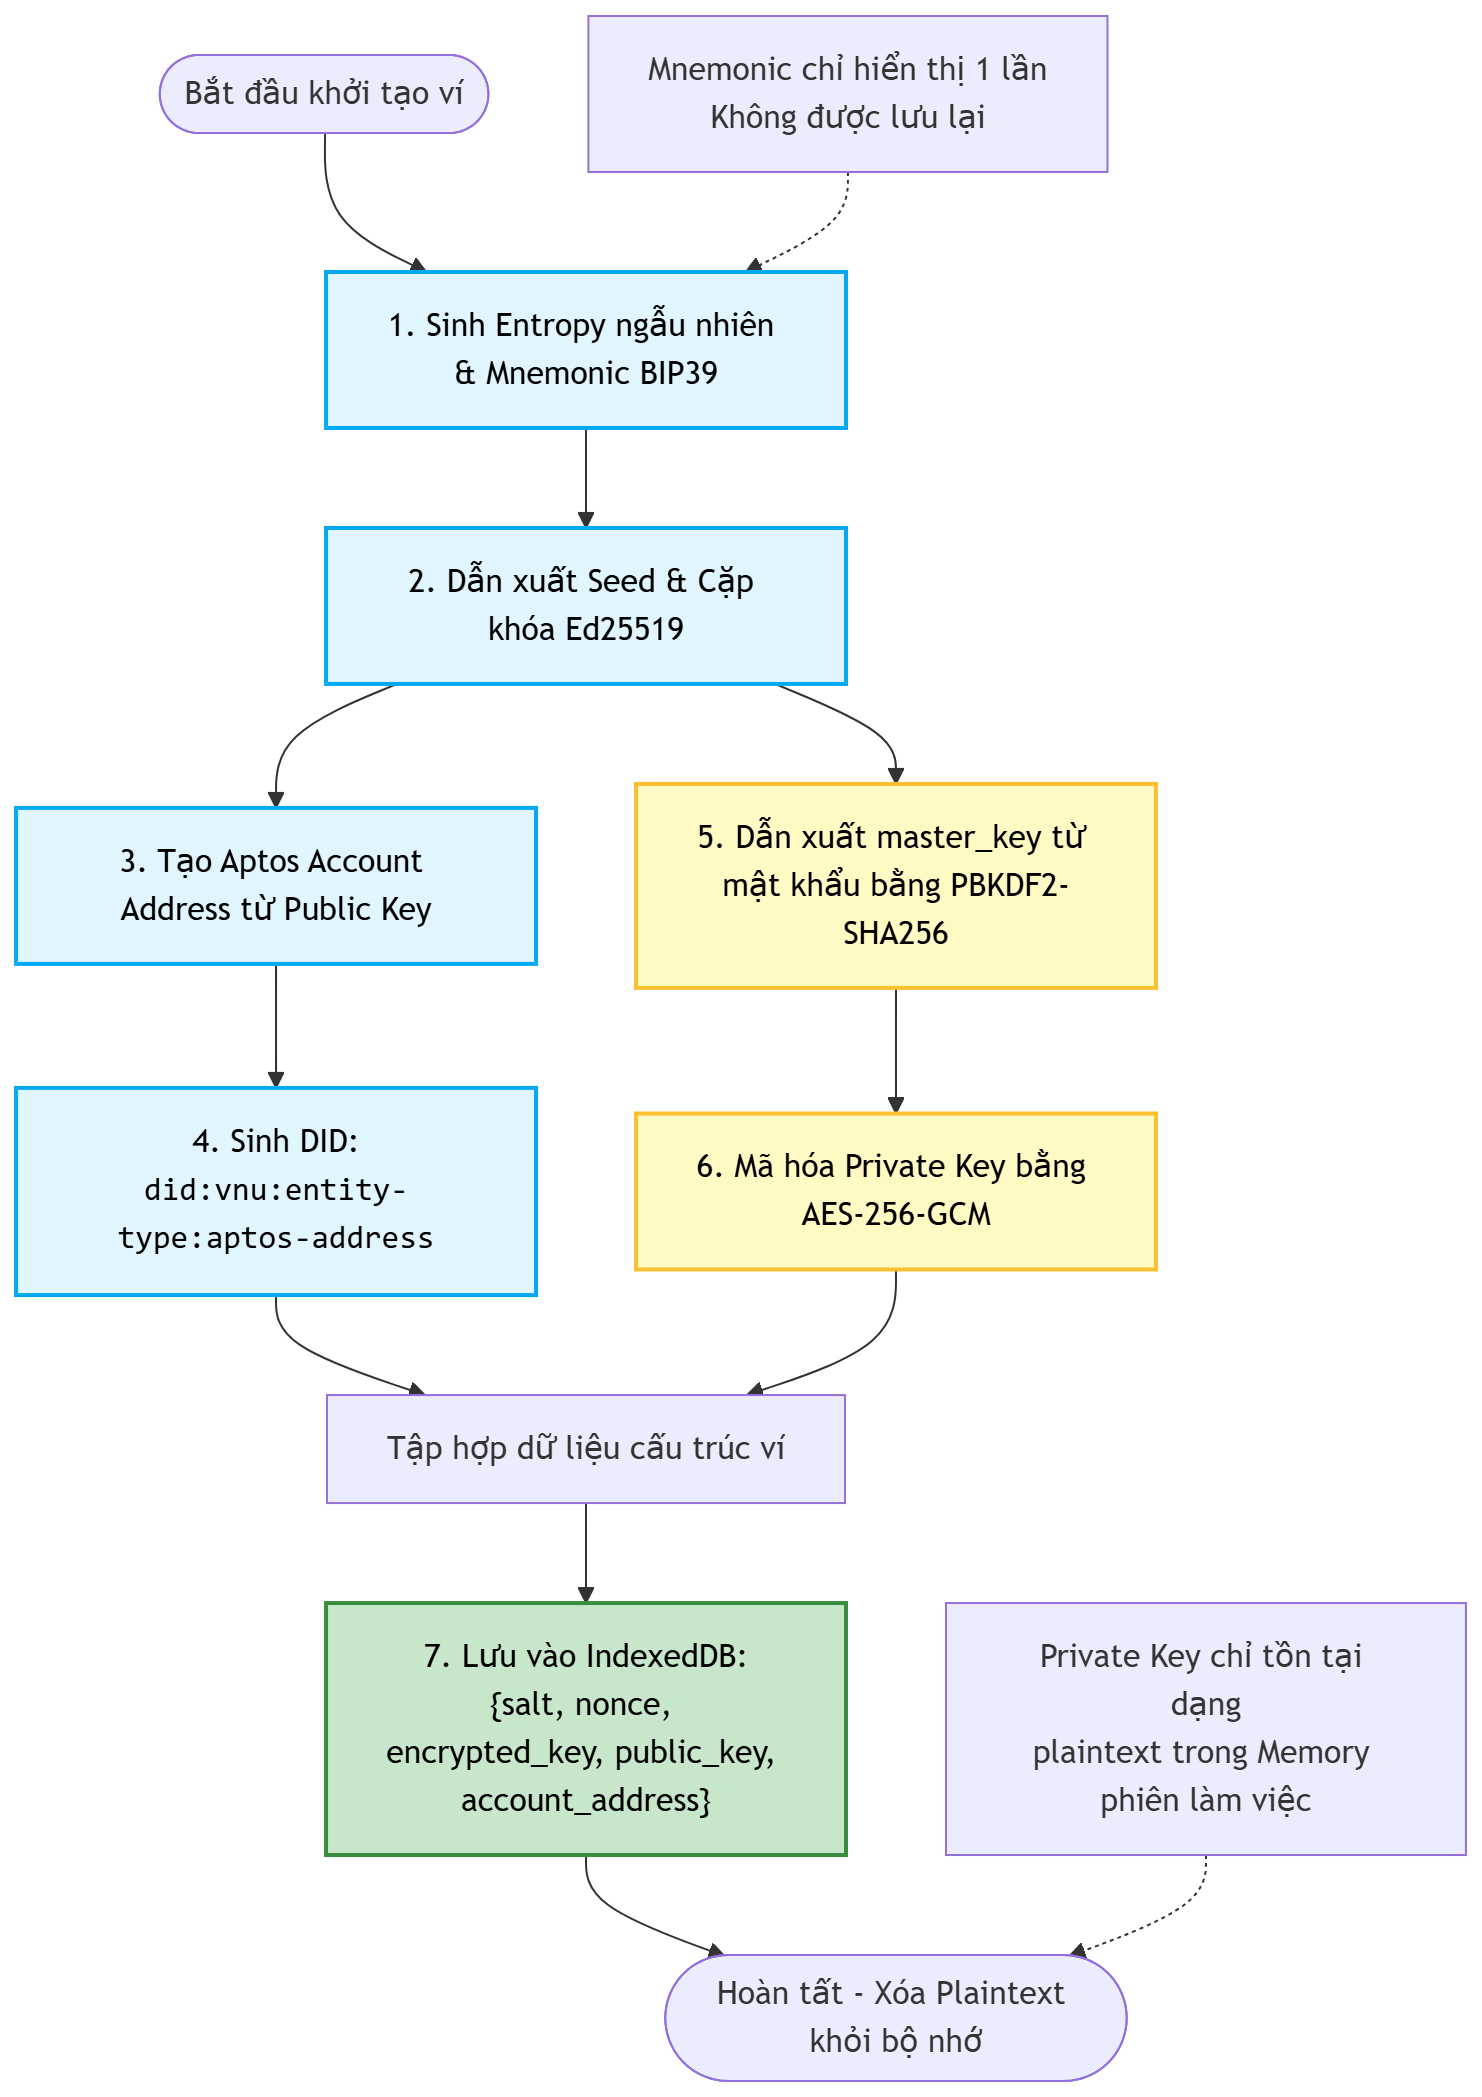
\includegraphics[width=0.5\textwidth]{images/khoi-tao-vi.png}
    \caption{Chuỗi bước sinh khóa và lưu trữ khi khởi tạo ví}
    \label{fig:khoi-tao-vi}
\end{figure}

Sau khi ví được khởi tạo, các thông tin nhạy cảm nằm ở dạng bản mã trong cơ sở dữ liệu cục bộ. Khi người dùng quay lại để đăng nhập, ký xác thực hoặc dựng bản trình bày, trình tự tương tác giữa các thành phần diễn ra như Hình \ref{fig:mo-khoa-va-su-dung}. Điểm cần chú ý trong sơ đồ: khóa riêng dạng rõ chỉ tồn tại trong bộ nhớ phiên làm việc và được giải phóng khi phiên kết thúc, nên bề mặt tấn công bị thu hẹp về đúng khoảng thời gian ví đang mở.

\begin{figure}[H]
    \centering
    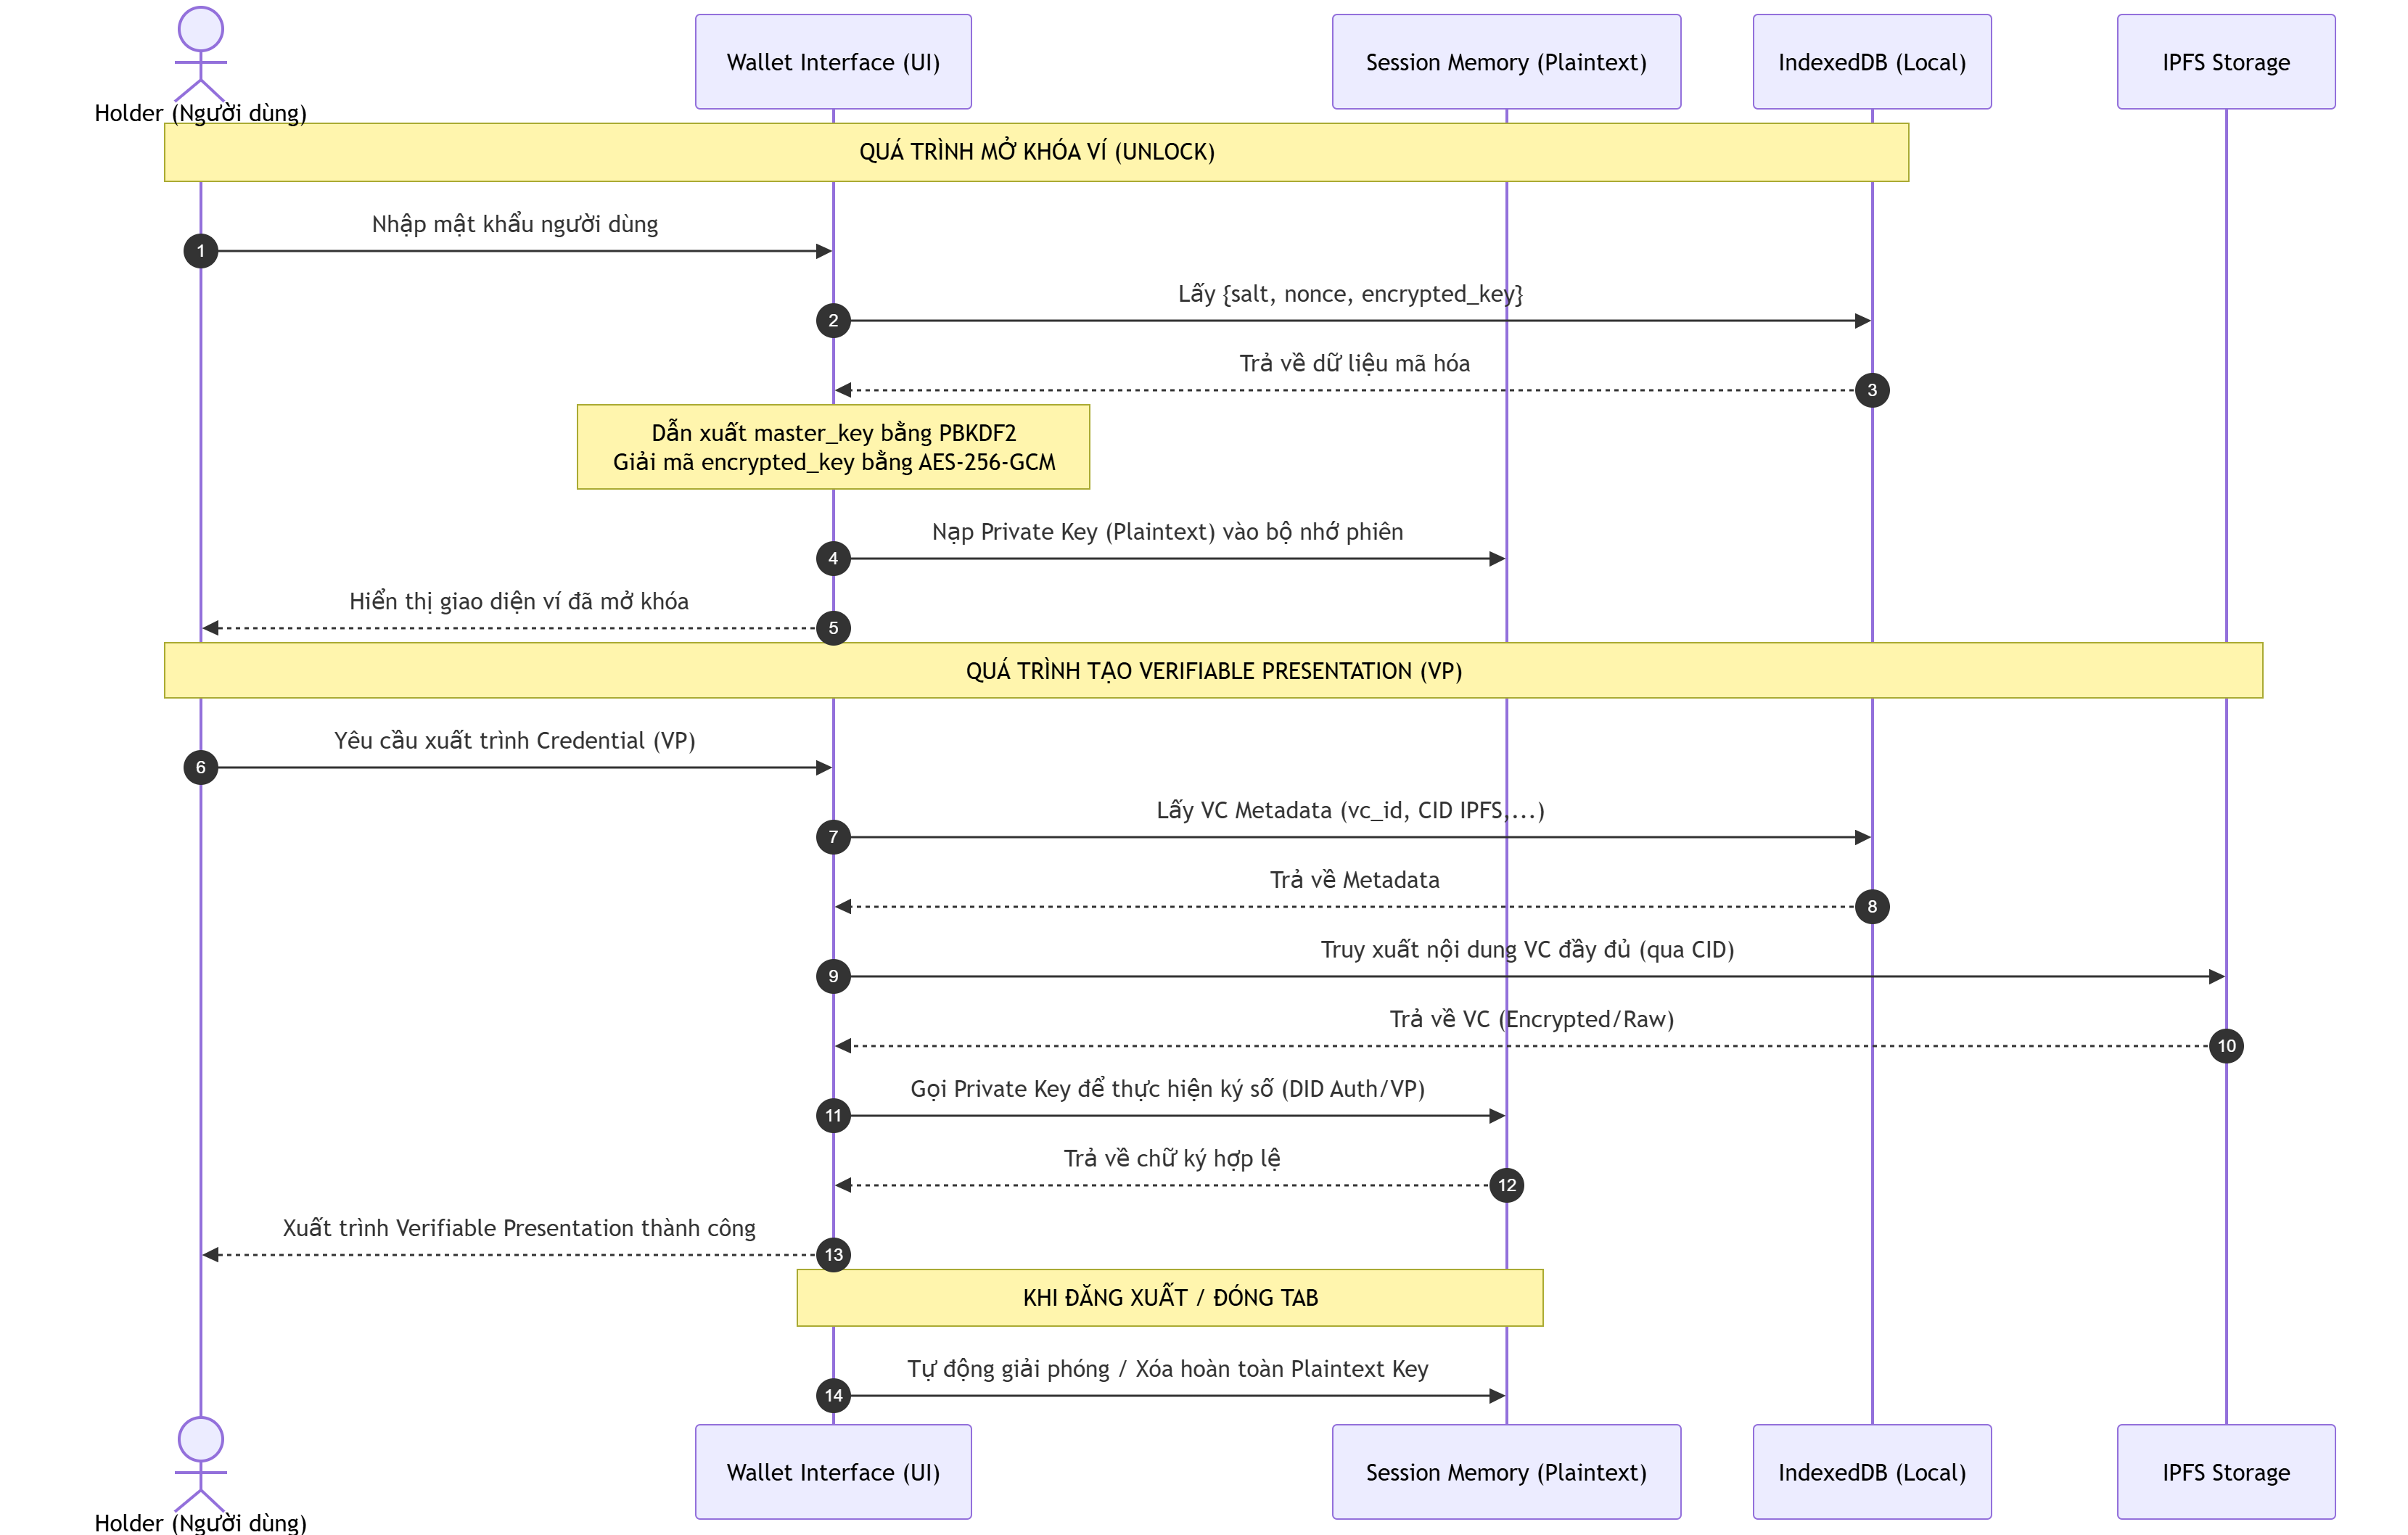
\includegraphics[width=1\textwidth]{images/mo-khoa-su-dung.png}
    \caption{Sơ đồ tuần tự khi mở khóa ví và dựng bản trình bày}
    \label{fig:mo-khoa-va-su-dung}
\end{figure}

Đánh đổi đã chấp nhận và được cảnh báo rõ trên giao diện: \textbf{mất mật khẩu là mất ví}, không có cơ chế đặt lại. Giao diện nhắc người dùng tải bản sao lưu ngay tại thời điểm tạo ví.

Một điểm cần nói rõ về những gì tầng dịch vụ lưu. Dịch vụ chỉ giữ \emph{bản ghi công khai} của mỗi thực thể: địa chỉ, khóa công khai, định danh, vai trò và nhãn hiển thị. Đó là một cuốn danh bạ, không phải một kho tài khoản --- không có giá trị băm mật khẩu, không có khóa riêng, không có cụm từ khôi phục. Hệ quả kiểm chứng được: biết địa chỉ của một người mà không có khóa riêng của họ thì không đăng nhập được.

\subsection{Khôi phục trên thiết bị khác}

Để chủ thể sử dụng được định danh của mình trên thiết bị khác, ví hỗ trợ khôi phục từ cụm từ ghi nhớ. Chuỗi dẫn xuất gồm bốn bước: mười hai từ theo từ điển BIP-39 \cite{BIP39} cho ra một hạt giống; hạt giống đi qua phép dẫn xuất phân cấp theo SLIP-0010 cho họ khóa Ed25519 \cite{SLIP0010} theo một đường dẫn xác định; từ đó suy ra khóa riêng và khóa công khai; và từ khóa công khai suy ra địa chỉ tài khoản.

Đường dẫn dẫn xuất được chọn trùng với đường dẫn mà các ví của hệ sinh thái Move sử dụng, nên một cụm từ ghi nhớ tạo bởi hệ thống này khôi phục được bằng ví phổ thông và ngược lại. Tính tương thích đó đã được kiểm chứng bằng cách đối chiếu kết quả dẫn xuất với bộ công cụ phát triển chính thức của nền tảng trên năm cụm từ ngẫu nhiên, với tiêu chí khớp tuyệt đối ở cả ba giá trị: khóa riêng, khóa công khai và địa chỉ.

Đây là một ví dụ của nguyên tắc kiểm chứng đã nêu ở Mục 1.5.2: giá trị kỳ vọng của phép kiểm không được tự đặt ra mà phải lấy từ một nguồn độc lập. Nếu bộ kiểm chỉ so kết quả dẫn xuất với một hằng số do chính người viết nghĩ ra, nó sẽ đạt kể cả khi phép dẫn xuất sai.

\subsection{Ký và gửi giao dịch không dùng bộ công cụ của nền tảng}

\noindent \textbf{Vấn đề}

Phiên bản đầu của giao diện có một ô {``}Mã giao dịch{''} ở mọi biểu mẫu: người dùng phải mở một ví ngoài, tự gọi hàm hợp đồng, chép mã giao dịch, rồi dán lại vào giao diện. Thiết kế này sai ở hai mức.

Ở mức trải nghiệm, nó đẩy phần khó nhất sang cho người dùng trong khi trình duyệt đã có sẵn khóa riêng trong bộ nhớ tab --- nếu trình duyệt ký được thì nó phải tự ký.

Ở mức dữ liệu, hệ quả nghiêm trọng hơn và không hiển nhiên: vì giao diện không tự gửi giao dịch, nó cũng \emph{không đọc được phản hồi của giao dịch}. Số hiệu của chứng thực do hợp đồng cấp nằm trong sự kiện mà giao dịch phát ra, và vì không đọc được sự kiện đó, trường số hiệu trên chuỗi bị ghi cứng bằng giá trị không --- một trường bịa nằm im trong cơ sở dữ liệu, trông như dữ liệu thật. Lỗi này chỉ lộ ra khi màn hình quản trị cần số hiệu đó để ký thao tác thu hồi.

Nhận định rút ra: thấy một ô {``}dán mã giao dịch{''} trong một giao diện có ví không lưu ký thì đó là dấu hiệu của thiết kế sai, không phải một yêu cầu nghiệp vụ.

\noindent \textbf{Ràng buộc: không thêm bộ công cụ của nền tảng}

Hướng xử lý hiển nhiên là nhúng bộ công cụ phát triển chính thức của nền tảng vào giao diện. Nhưng bộ công cụ đó có kích thước khoảng 4,7\,MB cho một vài phép ký, và việc nhúng nó đưa kích thước gói giao diện lên 4,98\,MB. Với một ứng dụng mà người dùng chủ yếu truy cập qua trình duyệt, đây là một cái giá không tương xứng.

Hướng đã chọn là thực hiện toàn bộ chuỗi thao tác bằng các thư viện mật mã độc lập, nhờ chính nút đầy đủ của mạng thực hiện phép tuần tự hóa nhị phân:

\begin{lstlisting}
POST /v1/transactions/encode_submission   <- giao dich chua ky
   -> chuoi thap luc phan cua thong diep can ky
ed25519.sign(thong diep, khoa rieng trong bo nho)
POST /v1/transactions                     <- giao dich + chu ky
   -> { hash }
GET  /v1/transactions/by_hash/{hash}       lap cho den khi xac nhan
\end{lstlisting}

Kết quả: kích thước gói giao diện giảm từ 4,98\,MB xuống 405\,KB. Đánh đổi là thêm một vòng gọi mạng cho mỗi giao dịch, để nút đầy đủ thực hiện phép tuần tự hóa. Trước khi chọn hướng này, các giá trị do thư viện mật mã độc lập sinh ra --- địa chỉ, khóa công khai và chữ ký --- đã được đối chiếu với bộ công cụ chính thức và cho kết quả khớp tuyệt đối.

\noindent \textbf{Kiểm chứng đường ký trên chuỗi thật}

Một đường ký tự hiện thực cần được kiểm chứng với chuỗi thật, nhưng việc kiểm chứng không nên tạo ra dữ liệu công khai ngoài ý muốn. Hệ thống dùng tuyến mô phỏng giao dịch của nút đầy đủ cho mục đích này. Tuyến này thực thi đầy đủ việc giải mã tham số, tìm hàm, vào thân hàm và tính chi phí, nên chứng minh được rằng cách mã hóa tham số và thứ tự tham số của giao diện là đúng --- mà không ghi bất cứ gì lên chuỗi.

Quá trình kiểm chứng này làm lộ ba chi tiết kỹ thuật không có trong tài liệu và đều từng gây lỗi:

\begin{itemize}
    \item \textbf{Tham số kiểu dãy byte phải được truyền ở dạng chuỗi thập lục phân}, không phải dạng mảng số. Truyền mảng số bị nút đầy đủ từ chối.
    \item \textbf{Nút đầy đủ từ chối mô phỏng một giao dịch có chữ ký hợp lệ.} Để mô phỏng, phải gửi một chữ ký toàn số không kèm khóa công khai \emph{thật} của người gửi.
    \item \textbf{Khóa xác thực trong thông tin tài khoản không phải khóa công khai} --- nó là giá trị băm của khóa công khai. Dùng sai giá trị này làm giao dịch bị từ chối vì khóa xác thực không hợp lệ.
\end{itemize}

\section{Giao diện theo vai trò}

Giao diện được tổ chức theo vai trò, với nguyên tắc: mỗi màn hình chỉ hiển thị những thao tác mà vai trò đó thực sự được phép thực hiện trên chuỗi. Điều này không thay thế việc kiểm quyền --- rào chắn thật vẫn ở hợp đồng --- nhưng tránh để người dùng thực hiện một thao tác chắc chắn thất bại.

Năm quy tắc phân quyền trên giao diện được lấy trực tiếp từ Bảng \ref{tab:role-permission}:

\begin{itemize}
    \item Ô chọn cấp bit ủy quyền bị khóa nếu người đang dùng không phải quản trị viên gốc.
    \item Các thao tác cấp và thu hồi quyền quản trị viên, đề cử người nhận quyền gốc chỉ xuất hiện ở màn hình quản trị gốc, và màn hình đó tự kiểm tra trên chuỗi rằng người đang dùng đúng là quản trị viên gốc.
    \item Thẻ ký nhận quyền gốc nằm ở trang cá nhân, không nằm trong khu quản trị --- vì tại thời điểm ký nhận, người đó vẫn chưa phải quản trị viên gốc.
    \item Nút kích hoạt lại chứng thực chỉ có ở màn hình quản trị viên, không có ở màn hình bên phát hành.
    \item Vai trò hiển thị trong ví được đồng bộ theo dịch vụ mỗi lần đăng nhập, nên một ví khai là chủ thể mà đã được cấp quyền quản trị viên sẽ thấy ngay các màn hình tương ứng.
\end{itemize}

Hai thành phần giao diện đáng được nêu vì chúng giải quyết các vấn đề vận hành thực tế.

\textbf{Thành phần tiến trình giao dịch} hiển thị năm bước của một thao tác ghi --- chuẩn bị dữ liệu, bảo đảm có chi phí giao dịch, ký, chờ chuỗi xác nhận, ghi chỉ mục --- mỗi bước một nhãn riêng. Mã giao dịch xuất hiện như \emph{kết quả} của thao tác kèm liên kết tới trình xem giao dịch, chứ không phải như dữ liệu người dùng phải nhập. Việc tách năm bước có giá trị chẩn đoán: khi thao tác thất bại, người dùng biết nó thất bại ở đâu, và ba nguyên nhân phổ biến nhất --- không đủ chi phí giao dịch, bị hợp đồng từ chối vì thiếu quyền, và chuỗi xác nhận chậm --- có ba cách xử lý khác nhau.

\textbf{Thẻ chi phí giao dịch} hiển thị số dư và một nút xin chi phí thử nghiệm cho chính tài khoản đang dùng. Thẻ này hiện cho mọi vai trò, kể cả chủ thể --- một lựa chọn cần giải thích, vì thoạt nhìn chủ thể không cần đến nó. Lý do: thao tác đăng ký định danh cũng tốn chi phí giao dịch, nên một chủ thể tự đăng ký định danh của mình vẫn cần. Cần nói rõ phạm vi của thành phần này: hệ thống \emph{không có} chức năng chuyển token --- không màn hình, không tuyến dịch vụ, không giao dịch chuyển token nào kể cả để thử nghiệm. Thao tác duy nhất liên quan tới token là việc xin chi phí giao dịch cho chính mình.

Khi chạy ở chế độ không phụ thuộc chuỗi, giao diện \emph{không} gửi giao dịch lên chuỗi, vì gói trên chuỗi có thể chưa tồn tại hoặc không khớp mã nguồn. Ví vẫn ký đúng nội dung giao dịch bằng khóa riêng thật, và tham chiếu gửi lên dịch vụ là giá trị băm của bản đã ký. Giao diện gọi đúng tên của giá trị này là \emph{tham chiếu cục bộ}, không gọi là mã giao dịch, và không đưa liên kết tới trình xem giao dịch. Đây là hệ quả của nguyên tắc ở Mục 4.4.4: một cờ chế độ phải được áp dụng nhất quán ở cả hai phía, và nguồn dữ liệu không được khai sai.

\section{Các kịch bản sử dụng}

Bảy kịch bản dưới đây bao phủ toàn bộ vòng đời văn bằng cùng các luồng quản trị, và được dùng làm căn cứ cho phần đánh giá ở Mục 4.8.

\subsection{Kịch bản 1: Đăng ký định danh}

\begin{figure}[H]
    \centering
    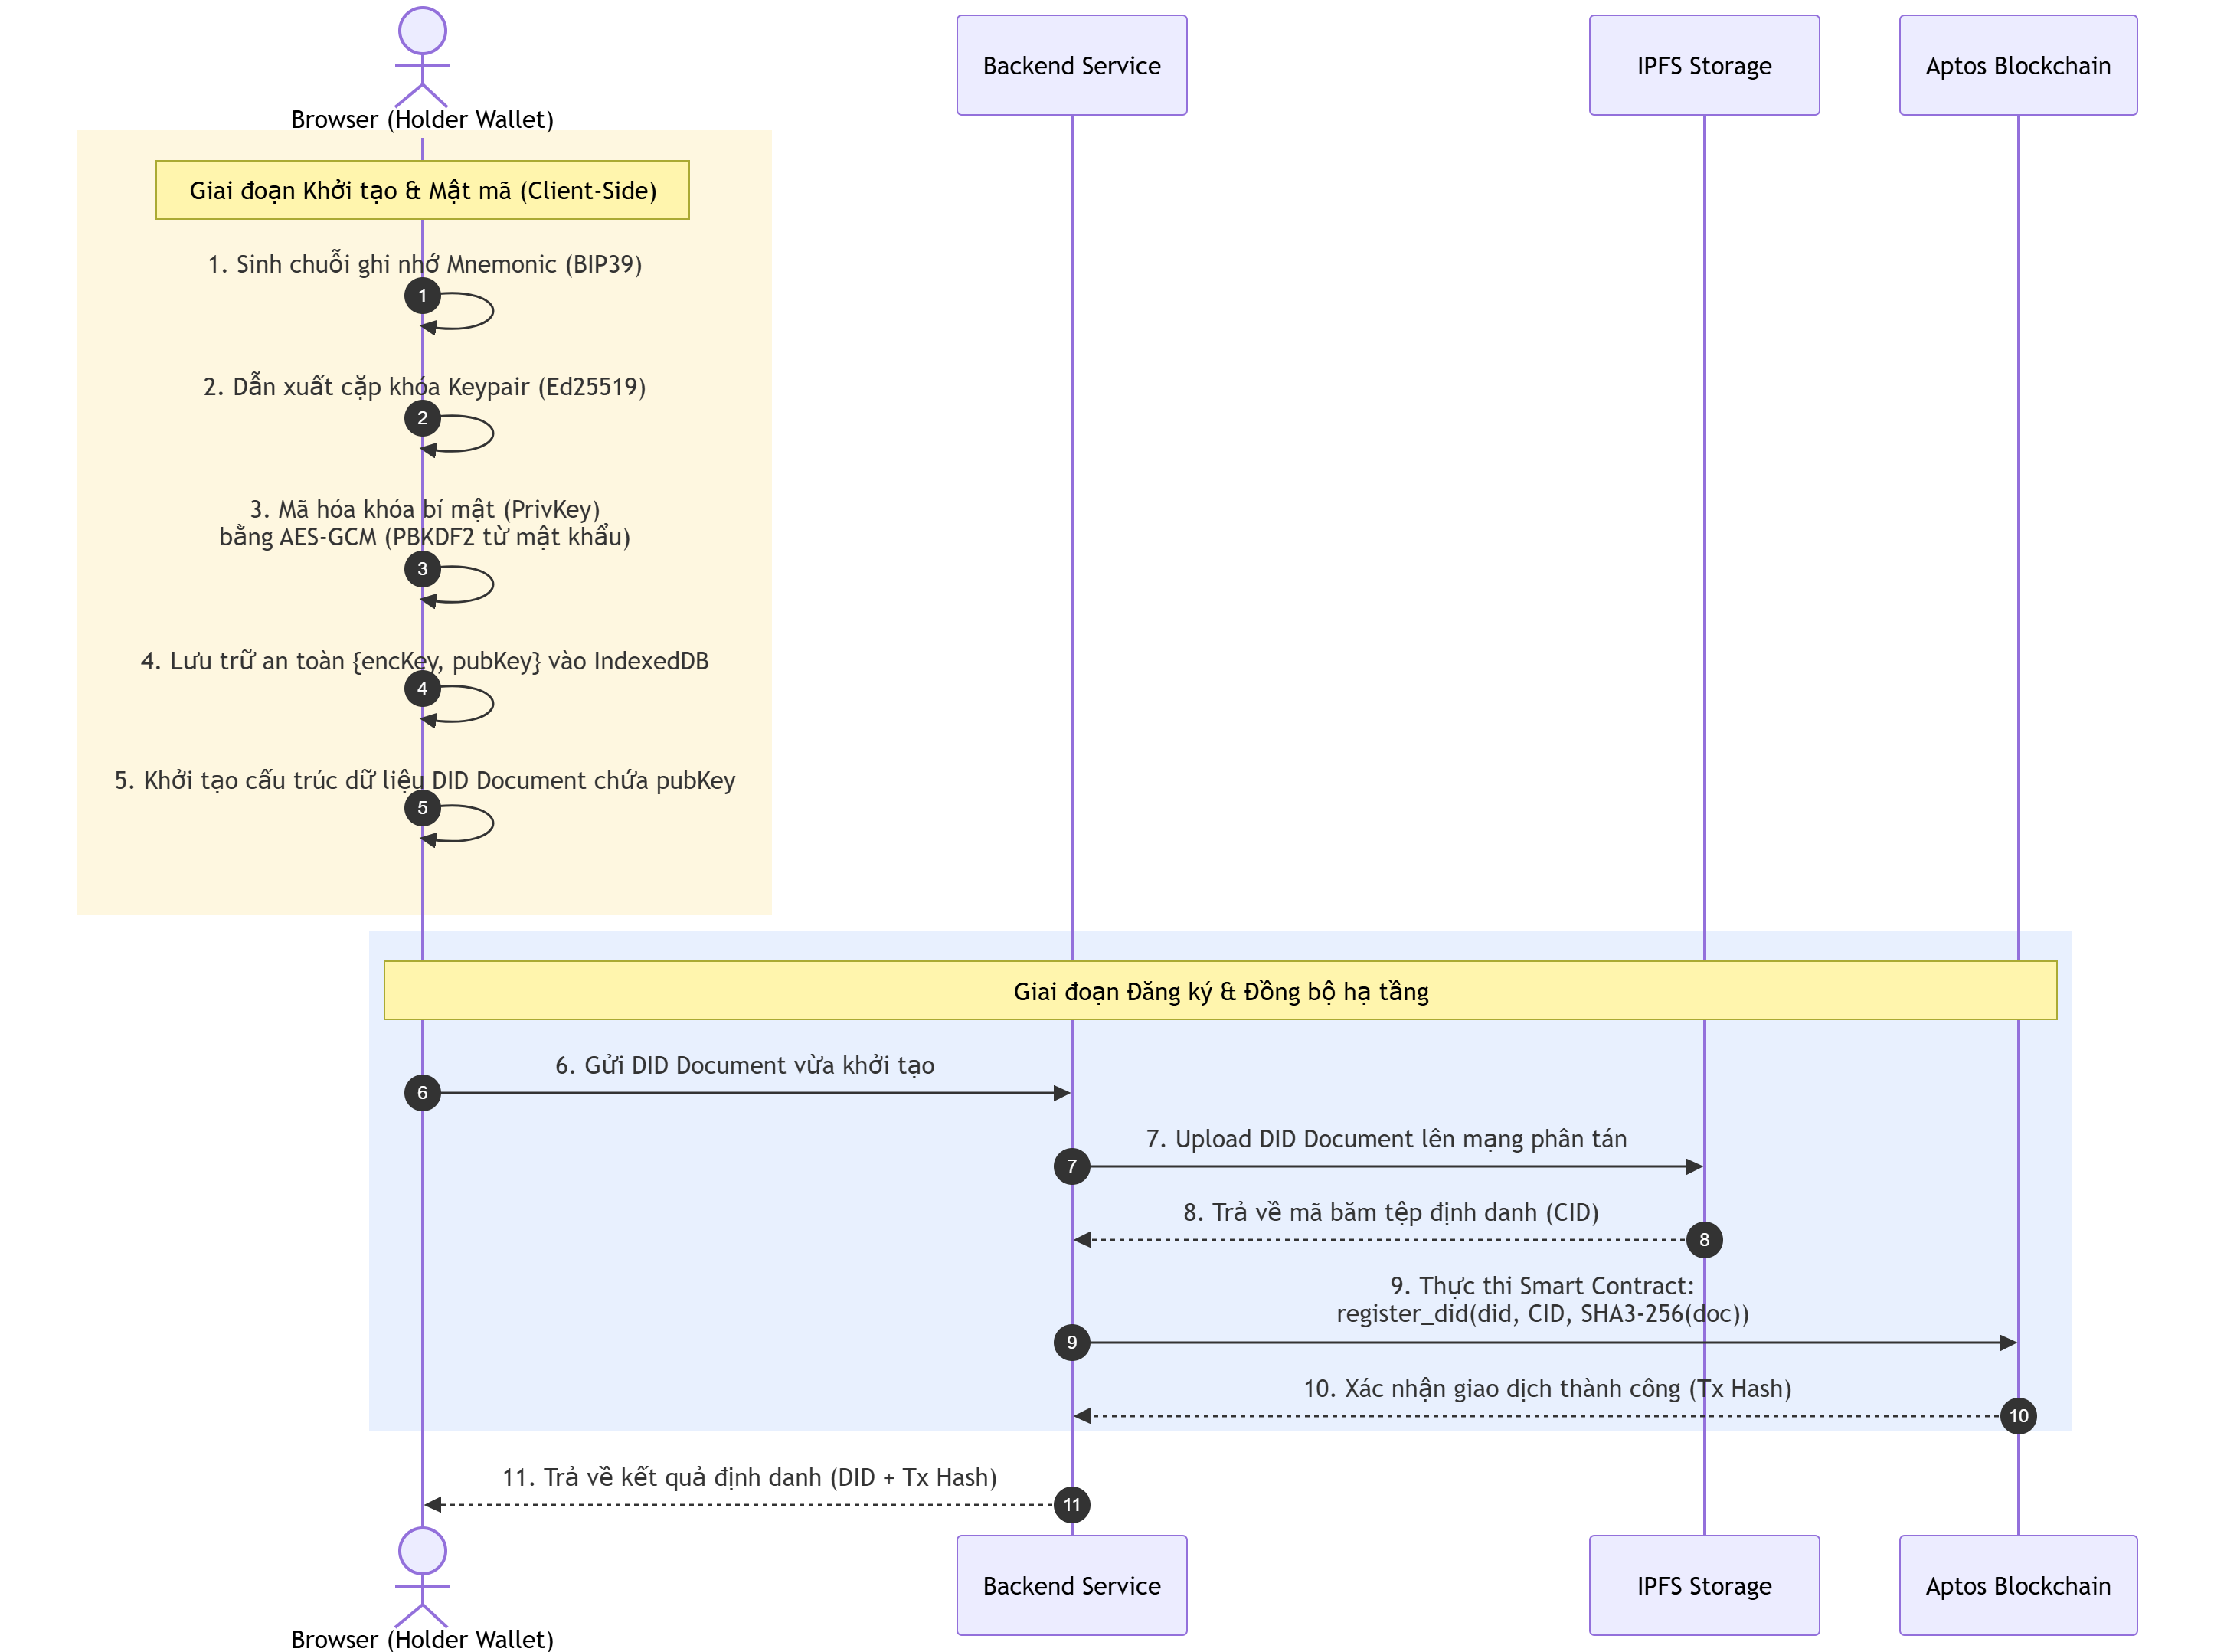
\includegraphics[width=1\textwidth]{images/seq_dang_ky_did_client.png}
    \caption{Sơ đồ tuần tự quy trình đăng ký định danh phía máy khách}
    \label{fig:seq_dang_ky_did_client}
\end{figure}

\begin{longtable}{|p{3.4cm}|p{10.3cm}|}
\caption{Đặc tả kịch bản đăng ký định danh}
\label{tab:did-registration-scenario} \\

\hline
\textbf{Mục} & \textbf{Nội dung} \\
\hline
\endfirsthead

\hline
\textbf{Mục} & \textbf{Nội dung} \\
\hline
\endhead

\hline
\endfoot

\hline
\endlastfoot

Mã kịch bản & KB1 \\
\hline

Tác nhân chính & Mọi vai trò: chủ thể, bên phát hành, quản trị viên, bên xác minh \\
\hline

Thành phần tham gia &
Ví định danh, tầng chuỗi phía máy khách, lớp lưu trữ ngoài chuỗi, mô-đun \cbox{did\_registry}, tầng chỉ mục \\
\hline

Mục đích &
Tạo một định danh phi tập trung và đăng ký siêu dữ liệu của nó lên chuỗi, để bất kỳ bên nào cũng phân giải được \\
\hline

Điều kiện tiên quyết &
\begin{itemize}[leftmargin=*, nosep]
    \item Ví đã được khởi tạo và đang ở trạng thái mở
    \item Địa chỉ của người dùng có đủ chi phí giao dịch
    \item Địa chỉ chưa có định danh đang hoạt động, hoặc định danh cũ đã bị thu hồi
\end{itemize} \\
\hline

Luồng thực hiện chính &
\begin{enumerate}[leftmargin=*, nosep]
    \item Ví dựng chuỗi định danh theo khuôn \cbox{did:vnu:<vai-tro>:<dia-chi>} từ địa chỉ của chính nó
    \item Ví dựng DID Document chứa khóa công khai, hai phương thức xác thực và khẳng định
    \item Giao diện tính giá trị băm SHA3-256 của tài liệu trên bản tuần tự hóa tất định
    \item Tài liệu được ghim lên lớp lưu trữ ngoài chuỗi, nhận về định danh nội dung
    \item Tầng chuỗi dựng giao dịch gọi \cbox{register\_did}, nhờ nút đầy đủ tuần tự hóa, ký bằng khóa riêng trong bộ nhớ, rồi gửi
    \item Giao diện chờ giao dịch được xác nhận và lấy mã giao dịch
    \item Tầng chỉ mục xác minh bốn điều của giao dịch rồi ghi bản ghi vào chỉ mục
\end{enumerate} \\
\hline

Luồng ngoại lệ &
\begin{itemize}[leftmargin=*, nosep]
    \item Ghim lên lớp lưu trữ thất bại $\rightarrow$ dừng ở bước chuẩn bị, không có giao dịch nào được gửi
    \item Không đủ chi phí giao dịch $\rightarrow$ giao diện gợi ý xin chi phí thử nghiệm rồi thử lại
    \item Chuỗi định danh đã tồn tại $\rightarrow$ hợp đồng từ chối với mã lỗi định danh đã được đăng ký
    \item Địa chỉ đã có định danh đang hoạt động $\rightarrow$ hợp đồng từ chối; phải thu hồi định danh cũ trước
    \item Giao dịch thất bại trên chuỗi $\rightarrow$ không có bản ghi nào được ghi vào chỉ mục
\end{itemize} \\
\hline

Kết quả sau cùng &
\begin{itemize}[leftmargin=*, nosep]
    \item Định danh được đăng ký với phiên bản 1 và trạng thái đang hoạt động
    \item Phân giải định danh thành công, giá trị băm tính lại khớp giá trị đã neo
\end{itemize} \\
\hline

Tính chất được kiểm chứng &
F1, F7, N5 --- khóa riêng không rời khỏi trình duyệt trong toàn bộ luồng \\
\hline

\end{longtable}


\subsection{Kịch bản 2: Phê duyệt bên phát hành}

\begin{longtable}{|p{3.4cm}|p{10.3cm}|}
\caption{Đặc tả kịch bản phê duyệt bên phát hành}
\label{tab:onboarding-issuer-scenario} \\

\hline
\textbf{Mục} & \textbf{Nội dung} \\
\hline
\endfirsthead

\hline
\textbf{Mục} & \textbf{Nội dung} \\
\hline
\endhead

\hline
\endfoot

\hline
\endlastfoot

Mã kịch bản & KB2 \\
\hline

Tác nhân chính & Quản trị viên gốc hoặc quản trị viên \\
\hline

Thành phần tham gia &
Ví của người quản trị, mô-đun \cbox{authority}, mô-đun \cbox{did\_registry}, lớp lưu trữ ngoài chuỗi, tầng chỉ mục \\
\hline

Mục đích &
Ghi một bản ghi thẩm quyền lên chuỗi, xác lập rằng một đơn vị được phép cấp một tập loại văn bằng xác định trong một thời hạn xác định \\
\hline

Điều kiện tiên quyết &
\begin{itemize}[leftmargin=*, nosep]
    \item Người thực hiện là quản trị viên gốc hoặc quản trị viên đang hoạt động trên chuỗi
    \item Đơn vị được phê duyệt đã có định danh đang hoạt động
    \item Đơn vị đó chưa giữ vai trò quản trị viên đang hoạt động
\end{itemize} \\
\hline

Luồng thực hiện chính &
\begin{enumerate}[leftmargin=*, nosep]
    \item Người quản trị chọn đơn vị và đánh dấu tập loại văn bằng được phép; giao diện gộp thành mặt nạ bit
    \item Ô chọn bit ủy quyền bị khóa nếu người thực hiện không phải quản trị viên gốc
    \item Người quản trị đặt thời hạn ủy quyền, hoặc để trống nếu vô thời hạn
    \item Nếu có quan hệ ủy quyền, chứng thực ủy quyền được ký và ghim lên lớp lưu trữ ngoài chuỗi
    \item Ví ký giao dịch gọi \cbox{approve\_issuer} với mặt nạ, thời hạn và tham chiếu chứng thực ủy quyền
    \item Hợp đồng kiểm các điều kiện, ghi bản ghi mới với phiên bản tăng thêm một, rồi phát sự kiện
    \item Tầng chỉ mục xác minh giao dịch, cập nhật vai trò trong chỉ mục và ghi nhật ký kiểm toán
\end{enumerate} \\
\hline

Luồng ngoại lệ &
\begin{itemize}[leftmargin=*, nosep]
    \item Người thực hiện không có quyền $\rightarrow$ hợp đồng từ chối với mã lỗi không phải quản trị viên
    \item Quản trị viên cố cấp bit ủy quyền $\rightarrow$ từ chối, chỉ quản trị viên gốc được cấp bit này
    \item Đơn vị chưa có định danh đang hoạt động $\rightarrow$ từ chối với mã lỗi định danh không hoạt động
    \item Đơn vị đang là quản trị viên $\rightarrow$ từ chối với mã lỗi xung đột vai trò
    \item Đơn vị đã là bên phát hành đang hoạt động $\rightarrow$ từ chối; phải thu hồi trước khi cấp lại
    \item Có quan hệ ủy quyền nhưng giá trị băm chứng thực ủy quyền sai độ dài $\rightarrow$ từ chối
\end{itemize} \\
\hline

Luồng thay thế: ủy quyền lại &
Một bên phát hành có bit ủy quyền thực hiện cùng thao tác cho đơn vị cấp dưới, với ba ràng buộc bổ sung do hợp đồng thi hành: phạm vi là tập con của phạm vi mình đang có, thời hạn không vượt thời hạn của mình, và bit ủy quyền không được truyền tiếp \\
\hline

Kết quả sau cùng &
\begin{itemize}[leftmargin=*, nosep]
    \item Bản ghi thẩm quyền tồn tại trên chuỗi và tra cứu được công khai
    \item Bản ghi cũ nếu có vẫn nằm trong tập bản ghi làm dấu vết kiểm toán
    \item Thao tác có mã giao dịch và có một dòng trong nhật ký kiểm toán
\end{itemize} \\
\hline

Tính chất được kiểm chứng &
F3, F4, F5, F12, N1, N2, N3 --- và các hành vi T1, T2 trong mô hình đe dọa \\
\hline

\end{longtable}


\subsection{Kịch bản 3: Cấp phát chứng thực}

\begin{figure}[H]
    \centering
    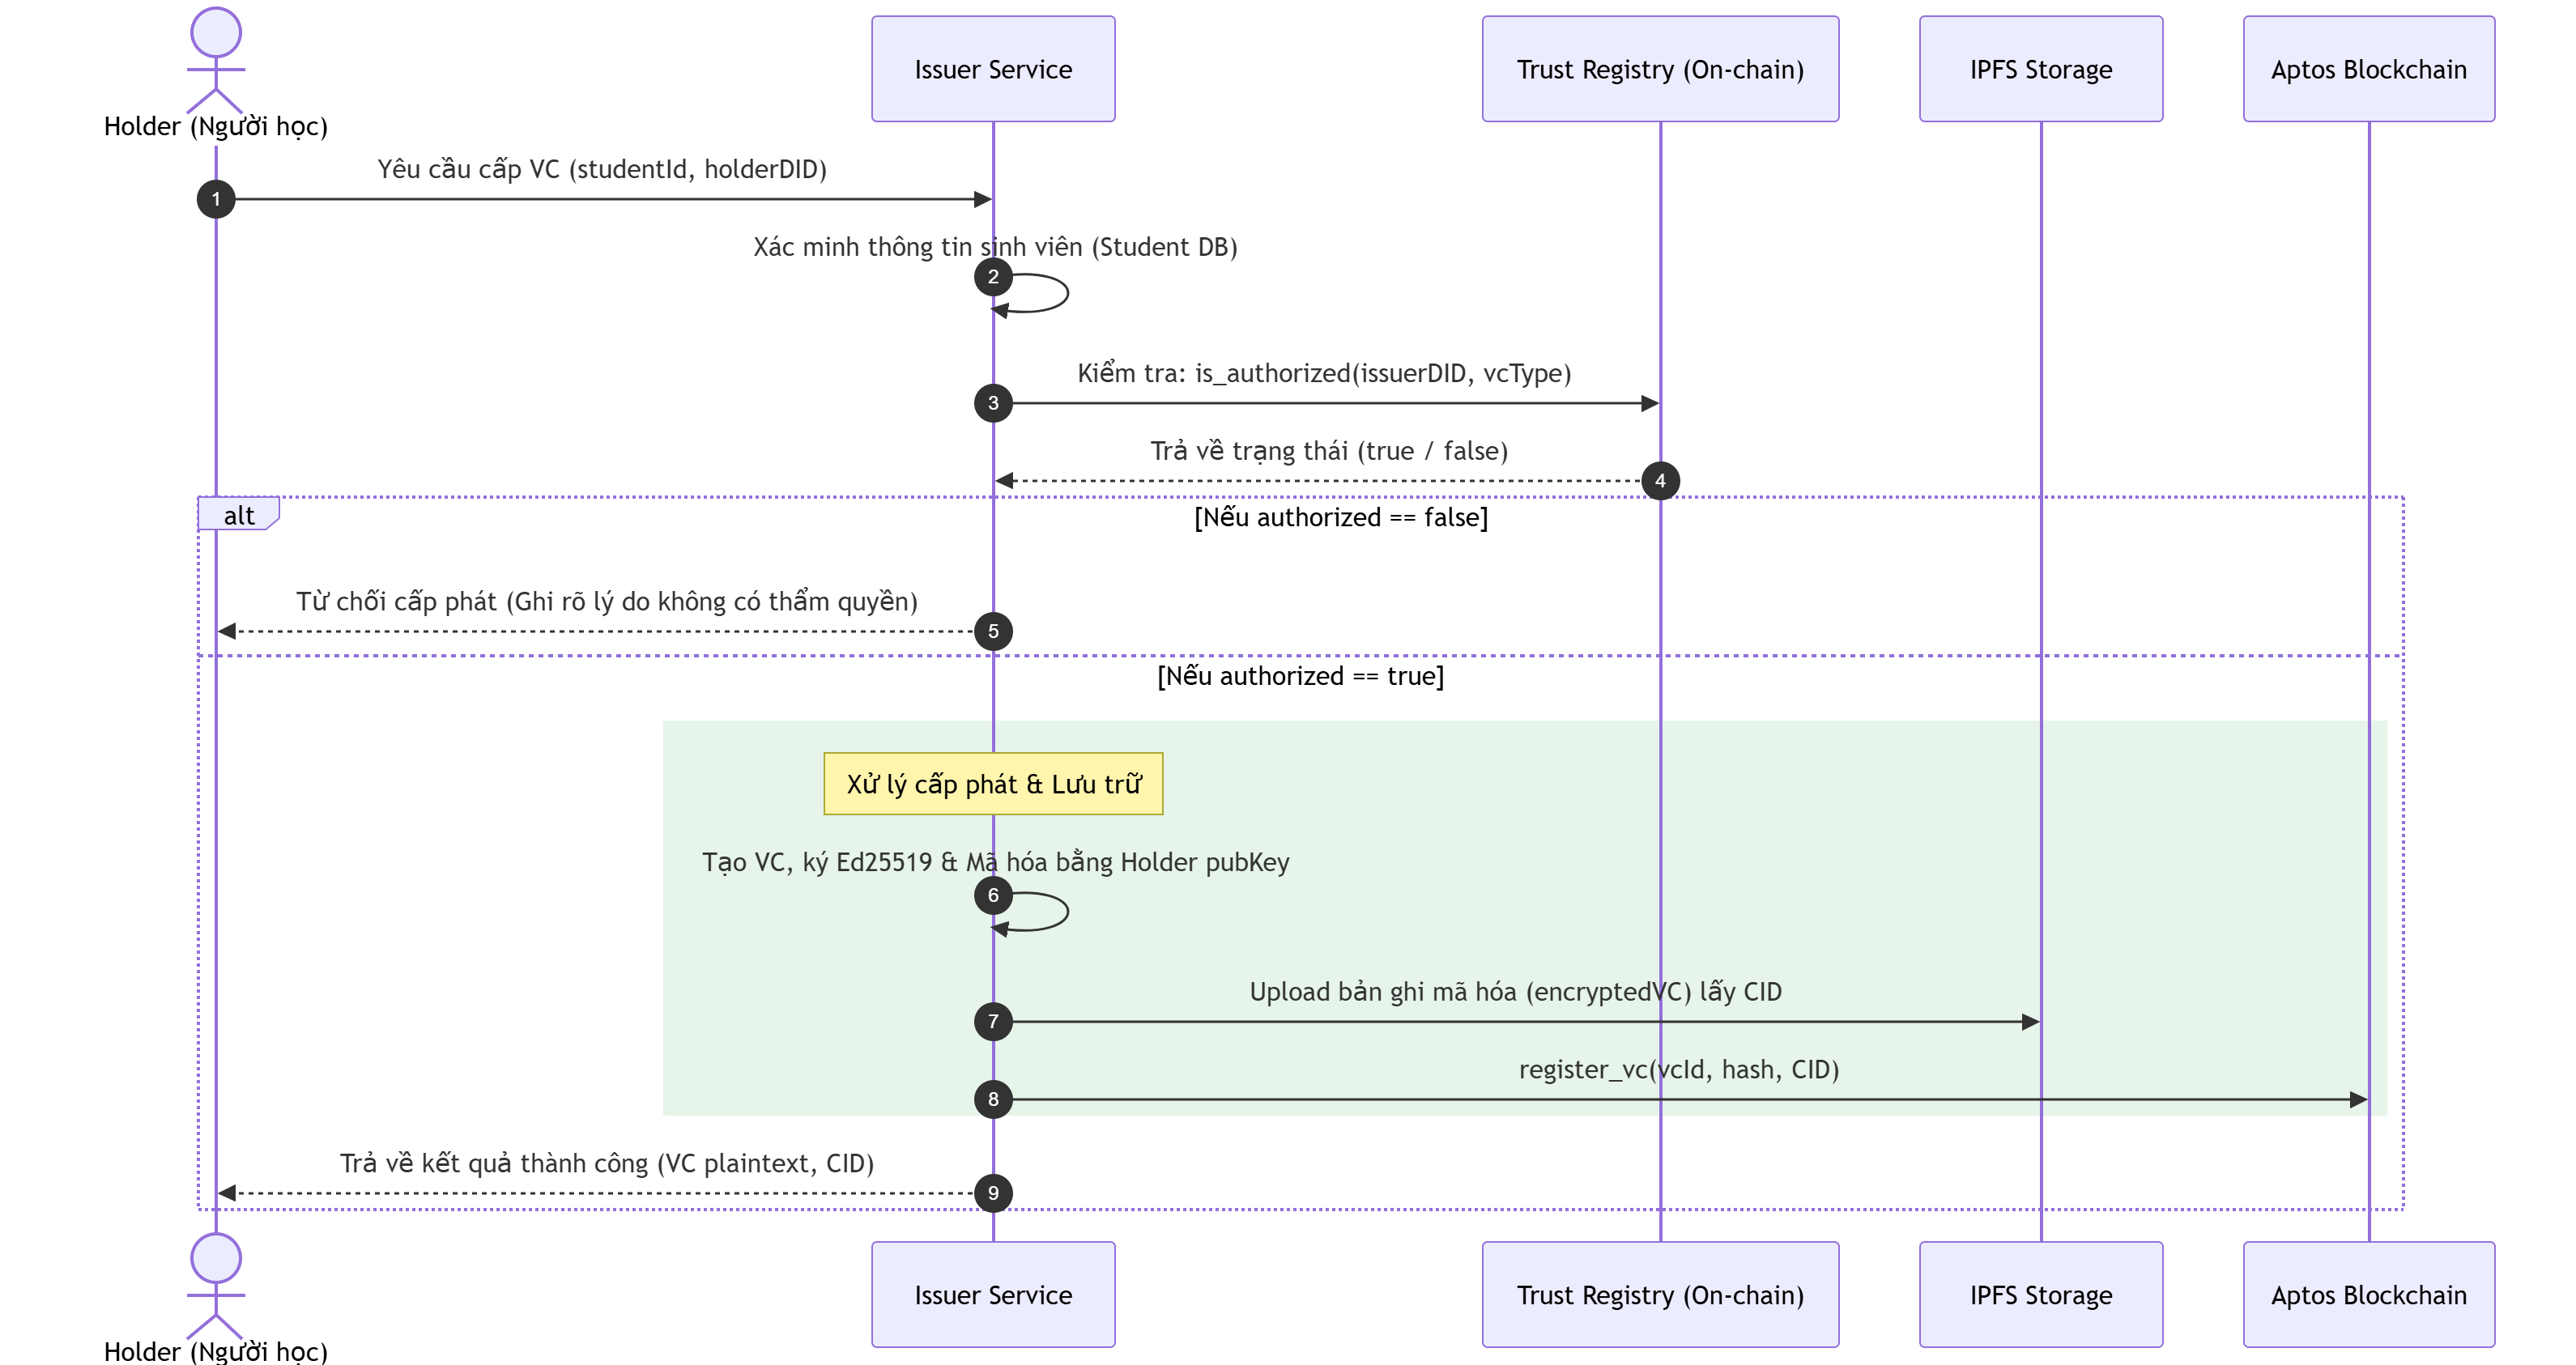
\includegraphics[width=1\textwidth]{images/seq_cap_phat_vc_authorized.png}
    \caption{Sơ đồ tuần tự quy trình cấp phát chứng thực}
    \label{fig:seq_cap_phat_vc_authorized}
\end{figure}

\begin{longtable}{|p{3.4cm}|p{10.3cm}|}
\caption{Đặc tả kịch bản cấp phát chứng thực}
\label{tab:vc-issuance-scenario} \\

\hline
\textbf{Mục} & \textbf{Nội dung} \\
\hline
\endfirsthead

\hline
\textbf{Mục} & \textbf{Nội dung} \\
\hline
\endhead

\hline
\endfoot

\hline
\endlastfoot

Mã kịch bản & KB3 \\
\hline

Tác nhân chính & Bên phát hành \\
\hline

Thành phần tham gia &
Ví của bên phát hành, lớp lưu trữ ngoài chuỗi, mô-đun \cbox{vc\_registry}, mô-đun \cbox{authority}, tầng chỉ mục \\
\hline

Mục đích &
Tạo một chứng thực văn bằng, ký bằng khóa riêng của bên phát hành, và neo giá trị băm của nó lên chuỗi \\
\hline

Điều kiện tiên quyết &
\begin{itemize}[leftmargin=*, nosep]
    \item Bên phát hành có bản ghi thẩm quyền đang hoạt động và chưa hết hạn
    \item Loại văn bằng cần cấp nằm trong phạm vi được phép
    \item Cả bên phát hành và chủ thể đều có định danh đang hoạt động
\end{itemize} \\
\hline

Luồng thực hiện chính &
\begin{enumerate}[leftmargin=*, nosep]
    \item Bên phát hành nhập dữ liệu văn bằng và định danh của chủ thể
    \item Giao diện dựng chứng thực theo mô hình dữ liệu W3C, với các thuộc tính riêng trong không gian tên của hệ thống
    \item Tính giá trị băm của nội dung chứng thực và giá trị băm của định danh chứng thực
    \item Ví ký nội dung chứng thực trên bản tuần tự hóa tất định
    \item Nội dung được ghim lên lớp lưu trữ ngoài chuỗi, nhận về định danh nội dung
    \item Ví ký giao dịch gọi \cbox{issue\_vc} với bảy tham số, trong đó có thời hạn
    \item Hợp đồng kiểm thẩm quyền, kiểm trạng thái định danh hai bên, kiểm độ dài các giá trị băm và định dạng định danh nội dung, rồi ghi bản ghi
    \item Giao diện đọc số hiệu chứng thực từ sự kiện trong phản hồi giao dịch
    \item Tầng chỉ mục xác minh giao dịch rồi ghi bản ghi kèm số hiệu thật
\end{enumerate} \\
\hline

Luồng ngoại lệ &
\begin{itemize}[leftmargin=*, nosep]
    \item Bên phát hành không có thẩm quyền $\rightarrow$ hợp đồng từ chối với mã lỗi bên phát hành không hoạt động
    \item Loại văn bằng ngoài phạm vi $\rightarrow$ từ chối với mã lỗi loại văn bằng không được phép
    \item Thẩm quyền đã hết hạn $\rightarrow$ từ chối với mã lỗi thẩm quyền đã hết hạn
    \item Định danh của chủ thể không hoạt động $\rightarrow$ từ chối
    \item Thời hạn chứng thực đặt vào quá khứ $\rightarrow$ từ chối, vì cấp một chứng thực đã hết hạn là vô nghĩa
    \item Giá trị băm của định danh chứng thực đã tồn tại $\rightarrow$ từ chối, chống cấp trùng
\end{itemize} \\
\hline

Kết quả sau cùng &
\begin{itemize}[leftmargin=*, nosep]
    \item Bản ghi chứng thực tồn tại trên chuỗi với trạng thái đang hoạt động
    \item Số hiệu chứng thực trong chỉ mục là số hiệu thật do hợp đồng cấp, đọc từ sự kiện
    \item Bộ đếm tổng đã cấp và bộ đếm số đang hiệu lực đều tăng
\end{itemize} \\
\hline

Tính chất được kiểm chứng &
F6, F12, N3, N4 --- và các hành vi T1, T2, T3, T9 trong mô hình đe dọa \\
\hline

\end{longtable}


\subsection{Kịch bản 4: Trình bày và xác minh}

\begin{longtable}{|p{3.4cm}|p{10.3cm}|}
\caption{Đặc tả kịch bản trình bày và xác minh}
\label{tab:vp-verification-scenario} \\

\hline
\textbf{Mục} & \textbf{Nội dung} \\
\hline
\endfirsthead

\hline
\textbf{Mục} & \textbf{Nội dung} \\
\hline
\endhead

\hline
\endfoot

\hline
\endlastfoot

Mã kịch bản & KB4 \\
\hline

Tác nhân chính & Chủ thể (trình bày) và bên xác minh (kiểm tra) \\
\hline

Thành phần tham gia &
Ví của chủ thể, lớp lưu trữ ngoài chuỗi, ba mô-đun hợp đồng, dịch vụ xác minh \\
\hline

Mục đích &
Chủ thể chứng minh mình sở hữu một tập văn bằng hợp lệ; bên xác minh kiểm chứng điều đó độc lập với bên phát hành \\
\hline

Điều kiện tiên quyết &
\begin{itemize}[leftmargin=*, nosep]
    \item Chủ thể có ít nhất một chứng thực trong ví
    \item Ví đang ở trạng thái mở
\end{itemize} \\
\hline

Luồng thực hiện chính &
\begin{enumerate}[leftmargin=*, nosep]
    \item Chủ thể chọn tập chứng thực muốn trình bày
    \item Giao diện dựng bản trình bày và ví ký bằng khóa riêng của chủ thể
    \item Bản trình bày được ghim lên lớp lưu trữ ngoài chuỗi
    \item Hệ thống sinh một liên kết chia sẻ có thời hạn, có thể thu hồi, kèm mã QR
    \item Bên xác minh mở liên kết và yêu cầu chạy quy trình xác minh
    \item Dịch vụ xác minh thực hiện bảy bước và trả báo cáo theo từng bước
    \item Bên xác minh có thể lưu kết quả vào lịch sử xác minh của mình
\end{enumerate} \\
\hline

Bảy bước kiểm tra &
\begin{enumerate}[leftmargin=*, nosep]
    \item Truy xuất bản trình bày từ lớp lưu trữ ngoài chuỗi
    \item Đối chiếu giá trị băm của bản trình bày
    \item Kiểm chữ ký của người trình bày bằng khóa công khai của chủ thể
    \item Kiểm trạng thái định danh của người trình bày
    \item Kiểm trạng thái hiệu lực của từng chứng thực, gồm cả thời điểm hết hạn
    \item Đối chiếu nội dung từng chứng thực với giá trị băm đã neo trên chuỗi
    \item Kiểm trạng thái thẩm quyền của bên phát hành từng chứng thực
\end{enumerate} \\
\hline

Luồng ngoại lệ &
\begin{itemize}[leftmargin=*, nosep]
    \item Liên kết chia sẻ đã hết hạn hoặc đã bị chủ thể thu hồi $\rightarrow$ dịch vụ từ chối truy cập
    \item Không tải được bản trình bày $\rightarrow$ bước một thất bại, và báo cáo phân biệt rõ đây là lỗi khả dụng chứ không phải lỗi hợp lệ
    \item Một hoặc nhiều bước thất bại $\rightarrow$ xem kịch bản KB7
\end{itemize} \\
\hline

Kết quả sau cùng &
\begin{itemize}[leftmargin=*, nosep]
    \item Báo cáo xác minh gồm trạng thái và chi tiết của cả bảy bước
    \item Kết quả tổng thể hợp lệ khi và chỉ khi cả bảy bước đạt
    \item Toàn bộ quy trình hoàn tất mà không cần liên hệ bên phát hành
\end{itemize} \\
\hline

Tính chất được kiểm chứng &
F8, F9, F10, N7, N8, N11 --- và các hành vi T7, T8, T15 trong mô hình đe dọa \\
\hline

\end{longtable}


\subsection{Kịch bản 5: Thu hồi thẩm quyền của bên phát hành}

\begin{longtable}{|p{3.4cm}|p{10.3cm}|}
\caption{Đặc tả kịch bản thu hồi thẩm quyền của bên phát hành}
\label{tab:issuer-revocation-scenario} \\

\hline
\textbf{Mục} & \textbf{Nội dung} \\
\hline
\endfirsthead

\hline
\textbf{Mục} & \textbf{Nội dung} \\
\hline
\endhead

\hline
\endfoot

\hline
\endlastfoot

Mã kịch bản & KB5 \\
\hline

Tác nhân chính & Quản trị viên gốc hoặc quản trị viên \\
\hline

Thành phần tham gia &
Ví của người quản trị, mô-đun \cbox{authority}, tầng chỉ mục, dịch vụ xác minh \\
\hline

Mục đích &
Đình chỉ hoặc thu hồi thẩm quyền cấp phát của một đơn vị, sao cho các lần xác minh sau đó phát hiện được trạng thái này \\
\hline

Điều kiện tiên quyết &
Người thực hiện là quản trị viên gốc hoặc quản trị viên đang hoạt động; đơn vị bị xử lý có bản ghi thẩm quyền \\
\hline

Phân biệt ba thao tác &
\begin{itemize}[leftmargin=*, nosep]
    \item \textbf{Đình chỉ}: trạng thái chuyển sang tạm đình chỉ. Quyền vẫn còn trong bản ghi, chỉ bị khóa. Vai trò trong chỉ mục \textbf{không đổi}
    \item \textbf{Kích hoạt lại}: đưa trạng thái từ tạm đình chỉ trở về đang hoạt động
    \item \textbf{Thu hồi}: trạng thái chuyển sang đã thu hồi. Vai trò trong chỉ mục hạ xuống chủ thể, nhưng đơn vị vẫn giữ định danh và các văn bằng của riêng mình
\end{itemize} \\
\hline

Luồng thực hiện chính &
\begin{enumerate}[leftmargin=*, nosep]
    \item Người quản trị chọn đơn vị, chọn thao tác và nhập lý do
    \item Ví ký giao dịch gọi hàm tương ứng trên mô-đun \cbox{authority}
    \item Hợp đồng cập nhật trạng thái, ghi lý do và dấu thời gian, rồi phát sự kiện
    \item Tầng chỉ mục xác minh giao dịch, cập nhật vai trò nếu cần và ghi nhật ký kiểm toán
    \item Từ thời điểm này, bước thứ bảy của quy trình xác minh phát hiện trạng thái mới
\end{enumerate} \\
\hline

Hệ quả đối với các chứng thực đã cấp &
\begin{itemize}[leftmargin=*, nosep]
    \item Các chứng thực do đơn vị đó cấp \textbf{vẫn hợp lệ về mặt kỹ thuật}: chữ ký vẫn đúng, nội dung vẫn khớp giá trị băm đã neo
    \item Nhưng chúng \textbf{bị từ chối ở bước kiểm thẩm quyền}, và báo cáo xác minh nêu rõ nguyên nhân là thẩm quyền của bên phát hành chứ không phải lỗi nội dung
    \item Đơn vị \textbf{vẫn thu hồi được} các chứng thực mình đã cấp, theo nguyên tắc bất đối xứng ở Mục 3.4.5
\end{itemize} \\
\hline

Luồng ngoại lệ &
\begin{itemize}[leftmargin=*, nosep]
    \item Người thực hiện không có quyền $\rightarrow$ hợp đồng từ chối
    \item Kích hoạt lại một đơn vị không ở trạng thái tạm đình chỉ $\rightarrow$ từ chối với mã lỗi tương ứng
    \item Thu hồi một đơn vị đã bị thu hồi $\rightarrow$ từ chối, tránh ghi hai bản ghi cho cùng một thao tác
\end{itemize} \\
\hline

Kết quả sau cùng &
Trạng thái mới tra cứu được công khai trên chuỗi; bản ghi cũ giữ nguyên làm dấu vết; thao tác có mã giao dịch và một dòng nhật ký \\
\hline

Tính chất được kiểm chứng &
F3, F10, F12, N1, N2 --- và nguyên tắc bất đối xứng ở Mục 3.4.5 \\
\hline

\end{longtable}


\subsection{Kịch bản 6: Thu hồi chứng thực}

\begin{longtable}{|p{3.4cm}|p{10.3cm}|}
\caption{Đặc tả kịch bản thu hồi chứng thực}
\label{tab:vc-revocation-scenario} \\

\hline
\textbf{Mục} & \textbf{Nội dung} \\
\hline
\endfirsthead

\hline
\textbf{Mục} & \textbf{Nội dung} \\
\hline
\endhead

\hline
\endfoot

\hline
\endlastfoot

Mã kịch bản & KB6 \\
\hline

Tác nhân chính & Bên phát hành (thu hồi, đình chỉ) hoặc quản trị viên (thu hồi, kích hoạt lại) \\
\hline

Thành phần tham gia &
Ví của người thực hiện, mô-đun \cbox{vc\_registry}, tầng chỉ mục, dịch vụ xác minh \\
\hline

Mục đích &
Cập nhật trạng thái của một chứng thực để các lần xác minh sau đó từ chối nó, dù chữ ký vẫn hợp lệ về mặt toán học \\
\hline

Điều kiện tiên quyết &
\begin{itemize}[leftmargin=*, nosep]
    \item Chứng thực tồn tại trên chuỗi
    \item Với thao tác của bên phát hành: người thực hiện đúng là bên đã cấp chứng thực đó, và định danh của họ còn hoạt động. \textbf{Không} yêu cầu thẩm quyền còn hiệu lực
    \item Với thao tác của quản trị viên: người thực hiện là quản trị viên gốc hoặc quản trị viên đang hoạt động
\end{itemize} \\
\hline

Phân biệt bốn thao tác &
\begin{itemize}[leftmargin=*, nosep]
    \item \textbf{Đình chỉ} (bên phát hành): trạng thái tạm thời, có thể đảo ngược --- nhưng chỉ quản trị viên đảo ngược được
    \item \textbf{Kích hoạt lại} (chỉ quản trị viên): đưa chứng thực từ tạm đình chỉ về đang hoạt động
    \item \textbf{Thu hồi} (bên phát hành): tuyên bố vĩnh viễn, không thể đảo ngược
    \item \textbf{Thu hồi} (quản trị viên): dùng khi cần cưỡng chế, chẳng hạn khi bên phát hành không còn hoạt động
\end{itemize} \\
\hline

Luồng thực hiện chính &
\begin{enumerate}[leftmargin=*, nosep]
    \item Người thực hiện chọn chứng thực trong bảng danh sách và chọn thao tác
    \item Giao diện đọc số hiệu chứng thực trên chuỗi từ chỉ mục --- số này không do người dùng gõ tay, để tránh gõ nhầm một chữ số và xử lý nhầm văn bằng của người khác
    \item Ví ký giao dịch gọi hàm tương ứng kèm lý do
    \item Hợp đồng kiểm điều kiện, cập nhật trạng thái, giảm bộ đếm số đang hiệu lực, rồi phát sự kiện
    \item Tầng chỉ mục xác minh giao dịch, cập nhật trạng thái trong chỉ mục và ghi nhật ký
\end{enumerate} \\
\hline

Hai trường hợp đặc biệt được hỗ trợ &
\begin{itemize}[leftmargin=*, nosep]
    \item \textbf{Đơn vị đã hết hạn ủy quyền vẫn thu hồi được} chứng thực mình đã cấp. Đây là kịch bản quan trọng nhất của nguyên tắc bất đối xứng: phát hiện gian lận thường xảy ra sau khi chu kỳ ủy quyền đã kết thúc
    \item \textbf{Chứng thực đã hết hạn vẫn thu hồi được}, vì hết hạn và thu hồi mang hai thông điệp khác nhau: hết hạn nói chứng thực không còn giá trị từ một thời điểm, thu hồi nói nó chưa bao giờ đáng tin
\end{itemize} \\
\hline

Luồng ngoại lệ &
\begin{itemize}[leftmargin=*, nosep]
    \item Người thực hiện không phải bên đã cấp $\rightarrow$ từ chối với mã lỗi không phải bên cấp
    \item Bên phát hành cố kích hoạt lại chứng thực $\rightarrow$ từ chối, thao tác này chỉ thuộc quản trị viên
    \item Thu hồi một chứng thực đã bị thu hồi $\rightarrow$ từ chối
    \item Định danh của bên thực hiện đã bị thu hồi $\rightarrow$ từ chối
\end{itemize} \\
\hline

Kết quả sau cùng &
Trạng thái mới tra cứu được trên chuỗi; bước thứ năm của quy trình xác minh từ chối chứng thực từ thời điểm này; bộ đếm số đang hiệu lực giảm \\
\hline

Tính chất được kiểm chứng &
F11, F12, N2 --- và các hành vi T13 trong mô hình đe dọa \\
\hline

\end{longtable}


\subsection{Kịch bản 7: Xác minh thất bại}

\begin{longtable}{|p{3.4cm}|p{10.3cm}|}
\caption{Đặc tả kịch bản xác minh thất bại}
\label{tab:verification-failure-scenario} \\

\hline
\textbf{Mục} & \textbf{Nội dung} \\
\hline
\endfirsthead

\hline
\textbf{Mục} & \textbf{Nội dung} \\
\hline
\endhead

\hline
\endfoot

\hline
\endlastfoot

Mã kịch bản & KB7 \\
\hline

Tác nhân chính & Bên xác minh \\
\hline

Mục đích &
Kiểm chứng rằng quy trình xác minh không chỉ từ chối đúng các trường hợp không hợp lệ, mà còn \textbf{nêu đúng nguyên nhân} --- điều kiện cần để bên xác minh biết phải xử lý thế nào \\
\hline

Nguyên tắc thiết kế được kiểm chứng &
Quy trình không dừng ở bước thất bại đầu tiên mà chạy hết cả bảy bước, rồi trả báo cáo đầy đủ. Lý do: một bản trình bày có thể hỏng ở nhiều chỗ, và bên xác minh cần thấy toàn bộ vấn đề \\
\hline

Trường hợp A: nội dung chứng thực bị sửa sau khi cấp &
Bước 6 (đối chiếu nội dung với giá trị băm đã neo) \textbf{thất bại}, trong khi bước 5 (trạng thái hiệu lực) và bước 7 (thẩm quyền bên phát hành) \textbf{vẫn đạt}. Đây là trường hợp quan trọng nhất của kịch bản: nó chứng minh một quy trình thiếu bước 6 sẽ chấp nhận chứng thực đã bị sửa. Tương ứng hành vi T7 \\
\hline

Trường hợp B: bản trình bày do thực thể khác ký &
Bước 3 (chữ ký của người trình bày) thất bại. Các bước còn lại có thể vẫn đạt, vì bản thân chứng thực không bị sửa gì. Tương ứng hành vi T8 \\
\hline

Trường hợp C: chứng thực đã bị thu hồi &
Bước 5 thất bại, nêu rõ trạng thái là đã thu hồi kèm lý do. Bước 6 vẫn đạt, vì nội dung không bị sửa --- đây là điểm phân biệt với trường hợp A \\
\hline

Trường hợp D: chứng thực đã hết hạn &
Bước 5 thất bại với trạng thái đã hết hạn. Báo cáo phân biệt rõ hết hạn với thu hồi, vì hai trạng thái này mang hai thông điệp khác nhau \\
\hline

Trường hợp E: bên phát hành đã bị thu hồi thẩm quyền &
Bước 7 thất bại. Các bước kỹ thuật đều đạt, vì chứng thực vẫn nguyên vẹn và chữ ký vẫn đúng. Tương ứng kịch bản KB5 \\
\hline

Trường hợp F: định danh của người trình bày đã bị thu hồi &
Bước 4 thất bại, nêu rõ trạng thái định danh. Trường hợp này tương ứng tình huống chủ thể đã thu hồi định danh cũ sau khi lộ khóa riêng \\
\hline

Trường hợp G: DID Document bị thay đổi trên lớp lưu trữ &
Phép đối chiếu giá trị băm trong quy trình phân giải định danh thất bại, nên bước 4 không hoàn tất. Tương ứng hành vi T15 \\
\hline

Trường hợp H: không tải được bản trình bày &
Bước 1 thất bại. Báo cáo phân biệt rõ đây là \textbf{lỗi khả dụng} chứ không phải \textbf{lỗi hợp lệ} --- một bản trình bày không tải được không có nghĩa là văn bằng không hợp lệ \\
\hline

Trường hợp I: liên kết chia sẻ hết hạn hoặc đã bị thu hồi &
Dịch vụ từ chối ngay ở bước mở liên kết, với mã trạng thái riêng phân biệt với lỗi không tìm thấy \\
\hline

Kết quả sau cùng &
\begin{itemize}[leftmargin=*, nosep]
    \item Mọi trường hợp đều bị từ chối ở kết quả tổng thể
    \item Báo cáo nêu đúng bước nào thất bại và vì nguyên nhân gì
    \item Ba nhóm nguyên nhân --- nội dung bị sửa, trạng thái không còn hiệu lực, thẩm quyền không còn --- được phân biệt rõ, theo Bảng \ref{tab:verification-matrix}
\end{itemize} \\
\hline

Tính chất được kiểm chứng &
F9, F10, N6 --- và các hành vi T7, T8, T15 trong mô hình đe dọa \\
\hline

\end{longtable}


\section{Chiến lược kiểm thử và kết quả kiểm chứng}

\subsection{Cấu trúc bộ kiểm thử}

Hệ thống được kiểm chứng bằng chín bộ kiểm thử ở các tầng khác nhau, mỗi bộ nhằm chứng minh một loại tính chất.

\begin{longtable}{|p{3.3cm}|c|p{8.4cm}|}
\caption{Chín bộ kiểm thử và tính chất mà mỗi bộ nhằm chứng minh}
\label{tab:test-suites} \\

\hline
\textbf{Bộ kiểm thử} & \textbf{Số phép} & \textbf{Tính chất được chứng minh} \\
\hline
\endfirsthead

\hline
\textbf{Bộ kiểm thử} & \textbf{Số phép} & \textbf{Tính chất được chứng minh} \\
\hline
\endhead

\hline
\endfoot

\hline
\endlastfoot

Kiểm thử đơn vị hợp đồng
& 126
& Logic phân quyền đúng đắn. Trong đó 83 phép dựng một thao tác vi phạm và khẳng định nó bị từ chối với đúng mã lỗi dự kiến
\\ \hline

Đối chiếu tên hàm hợp đồng
& 19
& Tên hàm khớp nhau giữa ba nơi gọi: mã Move, hai cài đặt tầng chỉ mục, và tầng chuỗi của giao diện
\\ \hline

Kiểm thử đầu cuối
& 19 $\times$ 2
& Các luồng chính hoạt động đầu cuối. Cùng một bộ chạy lên cả hai cài đặt qua biến môi trường chỉ địa chỉ dịch vụ
\\ \hline

Kiểm thử luồng nghiệp vụ
& 31 $\times$ 2
& Toàn bộ vòng đời văn bằng và các luồng quản trị, bao gồm nội dung thực của nhật ký kiểm toán
\\ \hline

Đối chiếu hai cài đặt
& 59
& Hai cài đặt trả cùng kết quả và cùng mã trạng thái cho cùng một yêu cầu, kể cả với dữ liệu vào không hợp lệ
\\ \hline

Phát hiện nội dung bị sửa
& 7 $\times$ 2
& Bước đối chiếu nội dung với giá trị băm đã neo phát hiện được nội dung bị sửa sau khi cấp, trong khi bước kiểm trạng thái vẫn đạt
\\ \hline

Kiểm thử chế độ nghiêm ngặt
& 6
& Ở chế độ phụ thuộc chuỗi, hệ thống vẫn chặn mã giao dịch bịa đặt và vẫn từ chối bên tự khai là bên phát hành
\\ \hline

Kiểm thử ví
& 17
& Khóa riêng không rời khỏi trình duyệt: kiểm toàn bộ gói tin gửi lên dịch vụ, không gói nào chứa khóa riêng hay mật khẩu
\\ \hline

Kiểm thử khôi phục thiết bị khác
& 17
& Khôi phục bằng cụm từ ghi nhớ cho đúng cặp khóa và địa chỉ; biết địa chỉ mà không có khóa thì đăng nhập thất bại
\\ \hline

Đối chiếu tầng chuỗi với nút đầy đủ
& 12
& Cách mã hóa tham số và thứ tự tham số của giao diện đúng với hợp đồng trên chuỗi thật, kiểm bằng tuyến mô phỏng nên không ghi gì lên chuỗi
\\ \hline

Phép đo tải
& 905.160 yêu cầu
& Hệ thống không sinh lỗi chức năng dưới tải; đồng thời lượng hoá chính độ tin cậy của phép đo (Mục 4.9)
\\ \hline

\end{longtable}


Ba đặc điểm của chiến lược này cần được nêu.

Thứ nhất, \textbf{phần lớn các phép kiểm trên hợp đồng là phép kiểm trường hợp vi phạm}. Trong 126 phép kiểm, có 83 phép --- tức khoảng 66\% --- dựng một thao tác vi phạm và khẳng định rằng nó bị từ chối với đúng mã lỗi dự kiến. Tỷ lệ này là có chủ đích, theo nhận định ở Mục 1.5.2: một quy tắc phân quyền chỉ được coi là hoạt động khi có một phép kiểm chứng minh nó thực sự chặn được điều nó tuyên bố chặn.

Thứ hai, \textbf{cùng một bộ kiểm thử đầu cuối được chạy lên cả hai cài đặt của tầng chỉ mục} thông qua một biến môi trường chỉ định địa chỉ dịch vụ. Đây là cách bảo đảm hai cài đặt thực sự tương đương, thay vì mỗi bên có một bộ kiểm riêng viết theo chính hành vi của nó.

Thứ ba, \textbf{bộ điều khiển kiểm thử cũng cần được kiểm thử}. Tập lệnh chạy toàn bộ bộ kiểm thử ban đầu dẫn đầu ra của mỗi bộ qua một lệnh lọc để in vài dòng cuối. Vì mã thoát của một đường ống trong vỏ lệnh là mã thoát của lệnh cuối cùng, và lệnh lọc luôn thành công, tập lệnh in {``}tất cả đạt{''} \emph{bất kể} có bộ nào thất bại. Lỗi này bị phát hiện khi một bộ báo 52 trên 53 phép đạt mà dòng tổng kết vẫn xanh. Sau khi sửa, cách kiểm chứng tập lệnh là cho một bộ thất bại có chủ ý và xác nhận rằng nó bị bắt.

\subsection{Kết quả kiểm chứng chức năng}

\begin{longtable}{|p{5.4cm}|p{3.1cm}|p{5.2cm}|}
\caption{Kết quả kiểm chứng chức năng ở lần chạy gần nhất}
\label{tab:test-results} \\

\hline
\textbf{Thành phần hoặc bộ kiểm} & \textbf{Kết quả} & \textbf{Ghi chú} \\
\hline
\endfirsthead

\hline
\textbf{Thành phần hoặc bộ kiểm} & \textbf{Kết quả} & \textbf{Ghi chú} \\
\hline
\endhead

\hline
\endfoot

\hline
\endlastfoot

Hợp đồng thông minh (Move)
& \textbf{126 / 126 đạt}
& Bao gồm 83 phép kiểm trường hợp vi phạm; mười vấn đề rà soát đều có phép kiểm chứng minh đã sửa \\
\hline

Đối chiếu tên hàm ba nơi gọi
& \textbf{19 / 19 khớp}
& Tăng từ 16 phép khi bổ sung tầng chuỗi của giao diện làm nơi gọi thứ ba \\
\hline

Tầng chỉ mục, cài đặt TypeScript
& 0 lỗi kiểm kiểu; \textbf{19 / 19} đầu cuối; \textbf{31 / 31} luồng nghiệp vụ
& Biên dịch ở chế độ kiểm kiểu nghiêm ngặt \\
\hline

Tầng chỉ mục, cài đặt Go
& Biên dịch và kiểm tĩnh sạch; \textbf{19 / 19} đầu cuối; \textbf{31 / 31} luồng nghiệp vụ
& Chạy cùng bộ kiểm thử với cài đặt TypeScript \\
\hline

Đối chiếu hai cài đặt
& \textbf{59 / 59 khớp}
& Tăng từ 53 phép sau khi bổ sung các tuyến còn thiếu ở cài đặt Go \\
\hline

Giao diện
& 0 lỗi kiểm kiểu; gói phát hành 405\,KB
& Giảm từ 4,98\,MB sau khi loại bộ công cụ của nền tảng \\
\hline

Kiểm thử ví
& \textbf{17 / 17 đạt}
& Gồm phép kiểm rằng không gói tin nào gửi lên dịch vụ chứa khóa riêng hoặc mật khẩu \\
\hline

Khôi phục trên thiết bị khác
& \textbf{17 / 17 đạt}
& Gồm phép kiểm rằng biết địa chỉ mà không có khóa thì đăng nhập bị từ chối \\
\hline

Phát hiện nội dung bị sửa
& \textbf{7 / 7 đạt} $\times$ 2 cài đặt
& Xem phân tích tại Mục 4.8.3 \\
\hline

Chế độ nghiêm ngặt
& \textbf{6 / 6 đạt}
& Chạy ở chế độ phụ thuộc chuỗi \\
\hline

Tầng chuỗi với nút đầy đủ
& \textbf{11 / 12 đạt}
& Phép còn lại thất bại vì gói trên chuỗi là bản xuất bản trước đợt sửa; xem phân tích tại Mục 4.8.2 \\
\hline

Phép đo tải, bốn thí nghiệm
& \textbf{0 lỗi / 905.160 yêu cầu}
& 0 phản hồi vượt hạn mức. Kết luận về ngưỡng độ trễ: xem Mục 4.9.6 \\
\hline

\end{longtable}


Hai kết quả cần được giải thích.

\textbf{Bộ đối chiếu tầng chuỗi với nút đầy đủ đạt 11 trên 12 phép.} Phép còn lại là phép đối chiếu tập hàm trong giao diện chương trình của gói \emph{đang nằm trên chuỗi} với tập hàm trong mã nguồn hiện tại. Phép này thất bại vì gói trên chuỗi là bản được xuất bản trước đợt sửa mười vấn đề rà soát: hàm cấp phát chứng thực trên chuỗi còn nhận sáu tham số thay vì bảy --- tức chưa có tham số thời hạn --- và hai hàm của cơ chế chuyển quyền gốc hai bước chưa tồn tại, trong khi hàm chuyển quyền một bước thì vẫn còn. Nói cách khác, phép kiểm này đang báo đúng một trạng thái thật và sẽ còn thất bại cho tới khi gói được xuất bản lại. Hệ quả đối với kết luận của chương: các kết quả về logic phân quyền ở Mục 4.8.3 được kiểm chứng trên bộ kiểm thử của hợp đồng --- tức trên mã nguồn đã sửa --- chứ không trên gói đang nằm trên chuỗi.

\textbf{Bộ đối chiếu tên hàm hợp đồng tăng từ 16 lên 19 phép} khi tầng chuỗi của giao diện được thêm vào làm nơi gọi thứ ba. Việc mở rộng này phát hiện ngay một sai lệch thật, đã nêu ở Mục 4.4.3. Nhận định rút ra: thêm một nơi gọi tên hàm hợp đồng thì phải mở rộng bộ bắt lệch ngay tại thời điểm đó, không phải khi nào nhớ ra.

\subsection{Kiểm chứng khả năng phát hiện gian lận}

Phần này đánh giá yêu cầu N6: mỗi kịch bản trong mô hình đe dọa ở Mục 3.7.2 phải bị chặn, và thông điệp từ chối phải khớp đúng nguyên nhân thật.

\begin{longtable}{|c|p{3.9cm}|p{3.4cm}|p{4.5cm}|}
\caption{Kết quả kiểm chứng khả năng phát hiện các hành vi trong mô hình đe dọa}
\label{tab:detection-results} \\

\hline
\textbf{Mã} & \textbf{Hành vi} & \textbf{Nơi bị chặn} & \textbf{Bộ kiểm chứng minh} \\
\hline
\endfirsthead

\hline
\textbf{Mã} & \textbf{Hành vi} & \textbf{Nơi bị chặn} & \textbf{Bộ kiểm chứng minh} \\
\hline
\endhead

\hline
\endfoot

\hline
\endlastfoot

T1 & Tự khai là bên phát hành rồi cấp văn bằng
& Hợp đồng, phép kiểm thẩm quyền
& Kiểm thử đơn vị hợp đồng; kiểm thử chế độ nghiêm ngặt
\\ \hline

T2 & Cấp loại văn bằng ngoài phạm vi
& Hợp đồng, phép giao bit
& Kiểm thử đơn vị hợp đồng
\\ \hline

T3 & Cấp văn bằng sau khi thẩm quyền hết hạn
& Hợp đồng, đối chiếu thời hạn
& Kiểm thử đơn vị hợp đồng
\\ \hline

T4 & Khai báo mã giao dịch không tồn tại
& Tầng dịch vụ, phép kiểm tồn tại
& Kiểm thử chế độ nghiêm ngặt
\\ \hline

T5 & Tái sử dụng giao dịch thật thuộc loại thao tác khác
& Tầng dịch vụ, so khớp tên hàm
& Kiểm thử chế độ nghiêm ngặt; đối chiếu tên hàm
\\ \hline

T6 & Tái sử dụng giao dịch của người khác
& Tầng dịch vụ, so khớp người gửi
& Kiểm thử chế độ nghiêm ngặt
\\ \hline

T7 & Sửa nội dung văn bằng sau khi cấp
& Quy trình xác minh, bước thứ sáu
& Bộ kiểm phát hiện nội dung bị sửa, cả hai cài đặt
\\ \hline

T8 & Trình bày chứng thực của người khác
& Quy trình xác minh, bước thứ ba
& Kiểm thử luồng nghiệp vụ
\\ \hline

T9 & Khai báo giá trị băm sai
& Tầng dịch vụ, tính lại giá trị băm
& Kiểm thử đầu cuối; đối chiếu hai cài đặt
\\ \hline

T10 & Gửi lại chữ ký đăng nhập đã thu được
& Tầng dịch vụ, số dùng một lần
& Kiểm thử ví; khôi phục thiết bị khác
\\ \hline

T11 & Lợi dụng vai trò trong phiên để vượt quyền
& Tầng dịch vụ và hợp đồng
& Kiểm thử chế độ nghiêm ngặt
\\ \hline

T12 & Gán quyền gốc cho địa chỉ không ai kiểm soát
& Hợp đồng, cơ chế hai bước
& Kiểm thử đơn vị hợp đồng
\\ \hline

T13 & Tự đình chỉ rồi tự kích hoạt lại chứng thực
& Hợp đồng, phân tách thẩm quyền
& Kiểm thử đơn vị hợp đồng; kiểm thử luồng nghiệp vụ
\\ \hline

T14 & Đăng ký chuỗi định danh đã thuộc thực thể khác
& Hợp đồng, phép kiểm duy nhất
& Kiểm thử đơn vị hợp đồng
\\ \hline

T15 & Cổng truy cập trả về nội dung khác nội dung đã đăng ký
& Quy trình phân giải, bước đối chiếu giá trị băm
& Bộ kiểm phát hiện nội dung bị sửa
\\ \hline

\end{longtable}


Hai bộ kiểm trong bảng trên được xây dựng riêng cho mục đích này và đáng được mô tả chi tiết hơn.

\textbf{Bộ kiểm phát hiện nội dung bị sửa} nhằm chứng minh rằng bước thứ sáu của quy trình xác minh không dư thừa. Bộ kiểm thực hiện ba việc: cấp một chứng thực và xác minh nó để xác nhận toàn bộ bảy bước đều đạt; sửa một trường trong nội dung chứng thực \emph{trực tiếp trong chỉ mục}, mô phỏng đúng kịch bản T7; rồi xác minh lại và khẳng định hai điều --- bước đối chiếu nội dung với giá trị băm đã neo \emph{thất bại}, và bước kiểm trạng thái hiệu lực \emph{vẫn đạt}. Khẳng định thứ hai là phần quan trọng: nó chứng minh rằng một quy trình xác minh chỉ theo dõi trạng thái sẽ bỏ sót đúng loại tấn công này, nên bước thứ sáu là cần thiết chứ không phải một phép kiểm thừa.

Quá trình xây dựng bộ kiểm này cũng làm lộ một vấn đề thuộc loại đã nêu ở Mục 4.4.5. Hàm đối chiếu nội dung với giá trị băm trên chuỗi đã tồn tại trong mã nguồn từ đầu, với một tên gọi nghe như đang bảo vệ tính toàn vẹn, nhưng \emph{không tuyến nào gọi tới nó} --- và ở cài đặt Go thì hàm đó không có. Người đọc mã sẽ tưởng nội dung chứng thực đang được đối chiếu với chuỗi, trong khi thực tế không. Một hàm được khai báo mà không ai gọi là một cái bẫy, vì nó tạo cảm giác an toàn mà không cung cấp sự an toàn.

\textbf{Bộ kiểm chế độ nghiêm ngặt} chứng minh rằng ở chế độ phụ thuộc chuỗi, hệ thống vẫn chặn mã giao dịch bịa đặt và vẫn từ chối bên tự khai là bên phát hành. Bộ kiểm này cần thiết vì phần lớn các bộ kiểm thử tự động khác chạy ở chế độ không phụ thuộc chuỗi để không cần mạng; nếu không có bộ kiểm riêng cho chế độ nghiêm ngặt, không có gì bảo đảm rằng các rào chắn ở chế độ đó còn hoạt động.

Trong quá trình xây dựng các bộ kiểm này, ba lớp lỗi phương pháp đã được xử lý và đáng ghi lại:

\begin{itemize}
    \item \textbf{Phép kiểm đạt chưa chắc vì lý do đúng.} Phép kiểm {``}mã giao dịch bịa đặt bị từ chối{''} ban đầu cho kết quả đạt, nhưng nguyên nhân thật là một định danh nội dung sai định dạng bị chặn trước, nên bước xác minh giao dịch chưa từng được thực thi. Mọi phép kiểm trường hợp vi phạm phải đọc thông điệp lỗi để xác nhận đúng nguyên nhân.
    \item \textbf{Dữ liệu giả phải đúng hình dạng dữ liệu thật.} Định danh nội dung giả phải tuân đúng khuôn dạng của định danh nội dung thật, nếu không nó bị chính bộ kiểm tra định dạng chặn trước khi chạm tới logic cần kiểm.
    \item \textbf{Phép kiểm thất bại vì hạ tầng thì không chứng minh được gì.} Bộ kiểm thử chạy nhiều kịch bản đăng nhập liên tiếp nên dính giới hạn tần suất một cách ngẫu nhiên. Vì không bộ nào khẳng định hành vi của giới hạn tần suất, tập lệnh chạy kiểm thử nâng giới hạn cho cả lượt chạy rồi trả lại --- thay vì rải các lệnh chờ và trông vào may mắn.
\end{itemize}

\section{Đánh giá hiệu năng}

\subsection{Thiết kế phép đo}

Phần đánh giá hiệu năng của bản thảo đầu tiên báo cáo một bảng số liệu thu từ \emph{một} lượt đo cho mỗi tuyến, ở \emph{một} mức đồng thời, với 120 yêu cầu mỗi tuyến. Khi rà soát lại, cách làm đó không trả lời được ba câu hỏi mà một phép đo cần trả lời trước khi con số của nó có nghĩa:

\begin{itemize}
    \item \textbf{Số đo có lặp lại được không?} Nếu chạy lại cùng phép đo cho con số khác hẳn, thì giá trị báo cáo là một mẫu ngẫu nhiên, không phải một đặc tính của hệ thống.
    \item \textbf{Hệ thống hành xử thế nào khi tải tăng?} Một con số ở một mức đồng thời không nói gì về điểm bão hoà.
    \item \textbf{Vì sao báo phân vị 95 mà không báo giá trị trung bình?} Đây là lựa chọn cần được chứng minh bằng dữ liệu, không phải bằng quy ước.
\end{itemize}

Vì vậy phép đo được thiết kế lại thành bốn thí nghiệm, tổng cộng \textbf{905.160 yêu cầu}:

\begin{enumerate}
    \item \textbf{Độ lặp lại} --- lặp cùng một phép đo 15 lượt cho mỗi tuyến và mỗi cài đặt, ở mức 12 yêu cầu đồng thời, để lượng hoá độ phân tán.
    \item \textbf{Ảnh hưởng của số mẫu} --- giữ nguyên mức đồng thời, thay đổi số mẫu mỗi lượt từ 60 đến 4000, mỗi mức lặp 12 lượt, nhằm phân biệt hai giả thuyết: độ trễ bản chất đã dao động, hay số mẫu quá ít.
    \item \textbf{Quét mức đồng thời} --- bảy mức từ 1 đến 64, mỗi điểm lặp 5 lượt với tối thiểu 1000 yêu cầu mỗi lượt, báo trung vị kèm khoảng nhỏ nhất--lớn nhất.
    \item \textbf{Phân bố độ trễ} --- một lượt lớn 1500 yêu cầu mỗi tuyến, giữ lại độ trễ của từng yêu cầu để dựng hàm phân bố tích luỹ.
\end{enumerate}

Toàn bộ dữ liệu thô được lưu dạng JSON, và các biểu đồ dưới đây được sinh tự động từ dữ liệu đó bằng một tập lệnh riêng. Việc tách bước đo khỏi bước vẽ có một lý do cụ thể: số liệu trong biểu đồ nhúng trực tiếp trong mã nguồn báo cáo nên kiểm chứng được từng con số, và vẽ lại không cần đo lại. Bốn thí nghiệm tương ứng với bốn tập lệnh trong mã nguồn --- \cbox{bench-sweep.mjs} cho thí nghiệm 1 và 4, \cbox{bench-samplesize.mjs} cho thí nghiệm 2, \cbox{bench-sweep2.mjs} cho thí nghiệm 3 --- và tập lệnh sinh biểu đồ là \cbox{bench-plot.mjs}.

Về môi trường đo, một đặc điểm quan trọng cần nêu trước vì nó quyết định cách đọc kết quả: bộ sinh tải, hai tiến trình dịch vụ và cơ sở dữ liệu \emph{cùng chạy trên một máy} có khoảng 3,9\,GB bộ nhớ. Bộ sinh tải vì vậy cạnh tranh tài nguyên với chính hệ thống đang được đo.

\subsection{Thí nghiệm 1: phép đo không lặp lại được ở số mẫu nhỏ}

% SINH TỰ ĐỘNG bởi scripts/bench-plot.mjs — đừng sửa tay.
% Nguồn dữ liệu: .bench/repeat.json
% Bảy cột với hai cột "x ± y" thì ở cỡ chữ thường sẽ tràn lề 92pt — thu nhỏ cỡ
% chữ và khoảng đệm cột thay vì cắt bớt cột, vì cột cuối chính là bằng chứng.
\begingroup
\footnotesize
\setlength{\tabcolsep}{4pt}
\begin{longtable}{|c|l|r|r|r|r|r|}
\caption{Độ lặp lại của phép đo: 15 lượt độc lập cho mỗi tuyến và mỗi cài đặt}
\label{tab:bench-repeat} \\

\hline
\textbf{Cài đặt} & \textbf{Tuyến} & \textbf{yc/giây} & \textbf{CV (\%)} & \textbf{p95 (ms)} & \textbf{CV (\%)} & \textbf{p95 min--max} \\
\hline
\endfirsthead

\hline
\textbf{Cài đặt} & \textbf{Tuyến} & \textbf{yc/giây} & \textbf{CV (\%)} & \textbf{p95 (ms)} & \textbf{CV (\%)} & \textbf{p95 min--max} \\
\hline
\endhead

\hline
\endfoot

\hline
\endlastfoot

TS & \texttt{/health} & 1146 $\pm$ 923 & 80.6 & 45.5 $\pm$ 33.1 & 72.7 & 6.8--139.2 \\
GO & \texttt{/health} & 2974 $\pm$ 1274 & 42.8 & 16.3 $\pm$ 19.0 & 116.2 & 4.7--59.3 \\
TS & \texttt{/stats} & 1470 $\pm$ 894 & 60.8 & 41.3 $\pm$ 31.1 & 75.2 & 5.1--105.5 \\
GO & \texttt{/stats} & 4229 $\pm$ 1808 & 42.7 & 13.2 $\pm$ 27.2 & 205.4 & 2.6--107.0 \\
TS & \texttt{/did/resolve} & 1326 $\pm$ 447 & 33.7 & 18.2 $\pm$ 8.2 & 44.9 & 9.0--32.5 \\
GO & \texttt{/did/resolve} & 2443 $\pm$ 874 & 35.8 & 15.3 $\pm$ 20.0 & 130.6 & 4.3--80.3 \\
TS & \texttt{/lookup} & 1525 $\pm$ 666 & 43.7 & 19.3 $\pm$ 14.5 & 75.3 & 5.8--56.9 \\
GO & \texttt{/lookup} & 2663 $\pm$ 1053 & 39.6 & 12.0 $\pm$ 11.2 & 93.0 & 4.5--47.8 \\
TS & \texttt{/auth/me} & 577 $\pm$ 225 & 39.1 & 40.1 $\pm$ 21.1 & 52.5 & 17.6--82.9 \\
GO & \texttt{/auth/me} & 1868 $\pm$ 661 & 35.4 & 16.2 $\pm$ 14.3 & 88.3 & 5.9--56.3 \\
TS & \texttt{/holder/credentials} & 1535 $\pm$ 335 & 21.8 & 16.6 $\pm$ 13.0 & 78.3 & 8.1--59.8 \\
GO & \texttt{/holder/credentials} & 2842 $\pm$ 1102 & 38.8 & 10.5 $\pm$ 9.1 & 86.7 & 4.3--40.3 \\

\end{longtable}
\endgroup


% SINH TỰ ĐỘNG bởi scripts/bench-plot.mjs — đừng sửa tay.
% Nguồn dữ liệu: .bench/repeat.json  (15 lượt mỗi tuyến, đo 2026-10-13T14:30:43.508Z)
\begin{figure}[H]
\centering
\begin{tikzpicture}
\begin{axis}[
    name=plotR,
    width=0.95\textwidth, height=5.4cm,
    ybar, bar width=7pt,
    xlabel={}, ylabel={Độ trễ p95 (ms)},
    xtick={0,1,2,3,4,5}, xticklabels={/health, /stats, /did/resolve, /lookup, /auth/me, /holder/credentials},
    x tick label style={font=\scriptsize, rotate=20, anchor=north east},
    tick label style={font=\footnotesize}, label style={font=\small},
    ymin=0,
    grid=both, grid style={gray!18},
    error bars/y dir=both, error bars/y explicit,
    legend style={font=\scriptsize, at={(0.98,0.98)}, anchor=north east, draw=gray!40},
    title={(a) p95 trung bình qua 15 lượt đo, thanh sai số là một độ lệch chuẩn},
    title style={font=\small},
]
    \addplot[fill=blue!35, draw=blue!60!black, error bars/error bar style={black}] coordinates {(0,45.52) +- (0,33.10) (1,41.32) +- (0,31.09) (2,18.17) +- (0,8.15) (3,19.28) +- (0,14.51) (4,40.12) +- (0,21.07) (5,16.62) +- (0,13.01)};
    \addlegendentry{TypeScript}
    \addplot[fill=orange!45, draw=orange!70!black, error bars/error bar style={black}] coordinates {(0,16.33) +- (0,18.97) (1,13.23) +- (0,27.17) (2,15.33) +- (0,20.01) (3,12.05) +- (0,11.21) (4,16.23) +- (0,14.34) (5,10.52) +- (0,9.12)};
    \addlegendentry{Go}
\end{axis}
\begin{axis}[
    at={(plotR.below south west)}, anchor=above north west, yshift=-0.9cm,
    width=0.95\textwidth, height=4.2cm,
    ybar, bar width=7pt,
    ylabel={Hệ số biến thiên của p95 (\%)},
    xtick={0,1,2,3,4,5}, xticklabels={/health, /stats, /did/resolve, /lookup, /auth/me, /holder/credentials},
    x tick label style={font=\scriptsize, rotate=20, anchor=north east},
    tick label style={font=\footnotesize}, label style={font=\small},
    ymin=0,
    grid=both, grid style={gray!18},
    legend style={font=\scriptsize, at={(0.98,0.98)}, anchor=north east, draw=gray!40},
    title={(b) Hệ số biến thiên --- càng cao thì số đo một lượt càng ít ý nghĩa},
    title style={font=\small},
]
    \addplot[fill=blue!35, draw=blue!60!black] coordinates {(0,72.7) (1,75.2) (2,44.9) (3,75.3) (4,52.5) (5,78.3)};
    \addlegendentry{TypeScript}
    \addplot[fill=orange!45, draw=orange!70!black] coordinates {(0,116.2) (1,205.4) (2,130.6) (3,93.0) (4,88.3) (5,86.7)};
    \addlegendentry{Go}
\end{axis}
\end{tikzpicture}
\caption{Độ lặp lại của phép đo độ trễ: cùng một phép đo (120 yêu cầu, 12 yêu cầu đồng thời) chạy lại 15 lần trên cùng một máy và cùng một cấu hình.}
\label{fig:bench-repeat}
\end{figure}


Kết quả rõ ràng và không thuận lợi cho bản thảo trước. Hệ số biến thiên của phân vị 95 --- tỉ số giữa độ lệch chuẩn và giá trị trung bình --- nằm trong khoảng \textbf{44,9\%} đến \textbf{205,4\%}, trung bình 93,3\%. Nói cách khác, ở mức 120 yêu cầu mỗi lượt, độ lệch chuẩn của p95 xấp xỉ bằng chính giá trị trung bình của nó.

Thông lượng ổn định hơn nhưng không nhiều: hệ số biến thiên 21,8--80,6\%, trung bình 42,9\%.

Hệ quả trực tiếp: \textbf{các giá trị p95 trong bảng số liệu của bản thảo đầu không phải là đặc tính của hệ thống mà là một mẫu ngẫu nhiên}. Chúng đã được loại khỏi báo cáo. Đây là một ví dụ của nguyên tắc đã nêu tại Mục 1.5.2 --- một phép đo không kiểm được độ lặp lại thì không chứng minh được điều gì --- và lần này nguyên tắc đó áp dụng cho chính phần đánh giá của nghiên cứu.

\subsection{Thí nghiệm 2: số mẫu giảm được nhiễu nhưng không loại bỏ được}

Thí nghiệm 1 cho thấy số đo dao động, nhưng chưa cho biết \emph{vì sao}. Có hai giả thuyết dẫn tới hai cách xử lý khác nhau: nếu độ trễ bản chất đã dao động thì phải báo p95 kèm độ lệch chuẩn; nếu 120 mẫu là quá ít thì chỉ cần tăng số mẫu.

% SINH TỰ ĐỘNG bởi scripts/bench-plot.mjs — đừng sửa tay.
% Nguồn dữ liệu: .bench/samplesize.json
\begin{table}[H]
\centering
\caption{Hệ số biến thiên của p95 theo số mẫu, tính trên 12 lượt đo độc lập (đơn vị \%)}
\label{tab:bench-samplesize}
\renewcommand{\arraystretch}{1.2}
\footnotesize
\begin{tabular}{|c|l|r|r|r|r|r|r|r|}
\hline
\multirow{2}{*}{\textbf{Cài đặt}} & \multirow{2}{*}{\textbf{Tuyến}} & \multicolumn{7}{c|}{\textbf{Số yêu cầu mỗi lượt đo}} \\
\cline{3-9}
 & & \textbf{60} & \textbf{120} & \textbf{250} & \textbf{500} & \textbf{1000} & \textbf{2000} & \textbf{4000} \\
\hline
TS & \texttt{/health} & 133.0 & 80.9 & 75.4 & 46.5 & 21.3 & 52.3 & 32.8 \\
GO & \texttt{/health} & 179.2 & 129.4 & 107.8 & 77.9 & 71.7 & 67.9 & 25.8 \\
TS & \texttt{/did/resolve} & 122.1 & 81.9 & 31.2 & 18.9 & 35.4 & 29.9 & 66.4 \\
GO & \texttt{/did/resolve} & 142.0 & 89.4 & 111.8 & 87.5 & 78.7 & 84.5 & 39.6 \\
TS & \texttt{/auth/me} & 74.5 & 28.5 & 99.2 & 125.5 & 66.5 & 20.9 & 54.6 \\
GO & \texttt{/auth/me} & 120.5 & 54.6 & 43.2 & 53.9 & 46.8 & 54.1 & 28.8 \\
\hline
\end{tabular}
\end{table}


% SINH TỰ ĐỘNG bởi scripts/bench-plot.mjs — đừng sửa tay.
% Nguồn dữ liệu: .bench/samplesize.json
% 12 lượt độc lập cho mỗi mức số mẫu, đồng thời 12, đo 2026-10-13T14:40:15.734Z
\begin{figure}[H]
\centering
\begin{tikzpicture}
\begin{axis}[
    name=ssA,
    width=0.95\textwidth, height=5.0cm,
    xlabel={}, ylabel={Hệ số biến thiên của p95 (\%)},
    xmode=log, log basis x=10,
    xtick={60,120,250,500,1000,2000,4000},
    xticklabels={60,120,250,500,1000,2000,4000},
    ymin=0,
    grid=both, grid style={gray!18},
    legend style={font=\tiny, at={(0.98,0.98)}, anchor=north east, fill=white, fill opacity=0.85, text opacity=1, draw=gray!40},
    label style={font=\small}, tick label style={font=\footnotesize},
    title={(a) Độ phân tán của p95 giảm khi tăng số mẫu}, title style={font=\small},
    extra y ticks={10}, extra y tick labels={}, extra y tick style={grid=major, grid style={red!45, densely dashed}},
]
    \addplot[color=blue!70!black,mark=*,mark size=1.5pt,thick] coordinates {(60,132.99) (120,80.88) (250,75.39) (500,46.47) (1000,21.31) (2000,52.26) (4000,32.85)};
    \addlegendentry{/health --- TS}
    \addplot[dashed,color=blue!70!black,mark=square*,mark size=1.5pt,thick] coordinates {(60,179.24) (120,129.36) (250,107.81) (500,77.86) (1000,71.70) (2000,67.87) (4000,25.75)};
    \addlegendentry{/health --- GO}
    \addplot[color=red!70!black,mark=*,mark size=1.5pt,thick] coordinates {(60,122.08) (120,81.86) (250,31.16) (500,18.93) (1000,35.38) (2000,29.87) (4000,66.35)};
    \addlegendentry{/did/resolve --- TS}
    \addplot[dashed,color=red!70!black,mark=square*,mark size=1.5pt,thick] coordinates {(60,142.01) (120,89.40) (250,111.76) (500,87.51) (1000,78.74) (2000,84.52) (4000,39.59)};
    \addlegendentry{/did/resolve --- GO}
    \addplot[color=green!55!black,mark=*,mark size=1.5pt,thick] coordinates {(60,74.50) (120,28.51) (250,99.15) (500,125.51) (1000,66.53) (2000,20.91) (4000,54.60)};
    \addlegendentry{/auth/me --- TS}
    \addplot[dashed,color=green!55!black,mark=square*,mark size=1.5pt,thick] coordinates {(60,120.54) (120,54.57) (250,43.21) (500,53.95) (1000,46.81) (2000,54.13) (4000,28.75)};
    \addlegendentry{/auth/me --- GO}
\end{axis}
\begin{axis}[
    at={(ssA.below south west)}, anchor=above north west, yshift=-0.9cm,
    width=0.95\textwidth, height=5.0cm,
    xlabel={Số yêu cầu mỗi lượt đo (thang logarit)}, ylabel={p95 trung bình (ms)},
    xmode=log, log basis x=10,
    xtick={60,120,250,500,1000,2000,4000},
    xticklabels={60,120,250,500,1000,2000,4000},
    ymin=0,
    grid=both, grid style={gray!18},
    legend style={font=\tiny, at={(0.98,0.98)}, anchor=north east, fill=white, fill opacity=0.85, text opacity=1, draw=gray!40},
    label style={font=\small}, tick label style={font=\footnotesize},
    title={(b) Giá trị p95 đo được cũng giảm --- mẫu nhỏ cho kết quả lệch cao}, title style={font=\small},
]
    \addplot[color=blue!70!black,mark=*,mark size=1.5pt,thick] coordinates {(60,17.51) (120,11.61) (250,13.90) (500,8.47) (1000,4.33) (2000,7.91) (4000,5.18)};
    \addlegendentry{/health --- TS}
    \addplot[dashed,color=blue!70!black,mark=square*,mark size=1.5pt,thick] coordinates {(60,25.06) (120,14.44) (250,9.34) (500,9.77) (1000,8.15) (2000,5.88) (4000,5.70)};
    \addlegendentry{/health --- GO}
    \addplot[color=red!70!black,mark=*,mark size=1.5pt,thick] coordinates {(60,11.28) (120,11.38) (250,6.95) (500,6.71) (1000,9.60) (2000,7.06) (4000,14.09)};
    \addlegendentry{/did/resolve --- TS}
    \addplot[dashed,color=red!70!black,mark=square*,mark size=1.5pt,thick] coordinates {(60,13.56) (120,10.56) (250,15.66) (500,8.28) (1000,16.36) (2000,17.93) (4000,9.56)};
    \addlegendentry{/did/resolve --- GO}
    \addplot[color=green!55!black,mark=*,mark size=1.5pt,thick] coordinates {(60,30.18) (120,14.11) (250,54.82) (500,141.00) (1000,36.56) (2000,20.70) (4000,49.90)};
    \addlegendentry{/auth/me --- TS}
    \addplot[dashed,color=green!55!black,mark=square*,mark size=1.5pt,thick] coordinates {(60,27.82) (120,13.57) (250,12.33) (500,33.40) (1000,20.05) (2000,18.00) (4000,12.66)};
    \addlegendentry{/auth/me --- GO}
\end{axis}
\end{tikzpicture}
\caption{Ảnh hưởng của số mẫu tới phép đo độ trễ. Mỗi điểm là trung bình của 12 lượt đo độc lập ở cùng mức 12 yêu cầu đồng thời. Đường gạch đỏ ở hình (a) là mức hệ số biến thiên 10\%.}
\label{fig:bench-samplesize}
\end{figure}


Dữ liệu ủng hộ giả thuyết thứ hai, nhưng chỉ một phần. Hệ số biến thiên trung bình của p95 giảm đơn điệu theo số mẫu:

\begin{center}
\footnotesize
\begin{tabular}{l|ccccccc}
Số mẫu mỗi lượt & 60 & 120 & 250 & 500 & 1000 & 2000 & 4000 \\
\hline
CV của p95 (\%) & 128,6 & 77,4 & 78,1 & 68,4 & 53,4 & 51,6 & 41,3 \\
\end{tabular}
\end{center}

Từ 128,6\% xuống 41,3\% --- giảm hơn ba lần. Giá trị p95 đo được cũng giảm theo, nghĩa là mẫu nhỏ không chỉ cho kết quả \emph{nhiễu} mà còn \emph{lệch cao}: với 60 mẫu, phân vị 95 là giá trị thứ 57 trong dãy đã sắp xếp, nên chỉ cần vài yêu cầu đầu tiên chậm vì chi phí thiết lập kết nối là đủ đẩy p95 lên.

Nhưng kết luận quan trọng hơn là phần \emph{không} được giải quyết: ngay ở 4000 mẫu mỗi lượt, hệ số biến thiên vẫn là 41,3\%, còn rất xa mức thường được coi là chấp nhận được. Tăng số mẫu làm giảm nhiễu nhưng không loại bỏ nó, nên nguồn nhiễu chi phối không phải số mẫu mà là \textbf{môi trường đo}: bộ sinh tải cạnh tranh tài nguyên với hệ thống đang được đo trên cùng một máy. Đây là một giới hạn của cách thiết lập thí nghiệm, không phải của hệ thống, và nó không khắc phục được bằng cách đo thêm.

\subsection{Thí nghiệm 3: hành vi khi tăng tải}

% SINH TỰ ĐỘNG bởi scripts/bench-plot.mjs — đừng sửa tay.
% Nguồn dữ liệu: .bench/sweep2.json
\begin{table}[H]
\centering
\caption{Kết quả quét mức đồng thời: 5 lượt mỗi điểm, tổng 265.200 yêu cầu}
\label{tab:bench-sweep}
\renewcommand{\arraystretch}{1.2}
\footnotesize
\begin{tabular}{|c|l|r|c|r|r|r|c|}
\hline
\textbf{Cài đặt} & \textbf{Tuyến} & \textbf{Đỉnh (yc/s)} & \textbf{tại c} & \textbf{p95 ở c=8} & \textbf{p95 trung vị lớn nhất} & \textbf{p95 lớn nhất} & \textbf{Lỗi} \\
\hline
TS & \texttt{/health} & 4078 & 4 & 4.6 & 52.6 & 76.5 & 0 \\
GO & \texttt{/health} & 4797 & 32 & 3.5 & 39.3 & 894.9 & 0 \\
TS & \texttt{/did/resolve} & 2217 & 4 & 10.9 & 131.6 & 172.3 & 0 \\
GO & \texttt{/did/resolve} & 3509 & 8 & 3.8 & 141.2 & 539.1 & 0 \\
TS & \texttt{/auth/me} & 721 & 2 & 38.1 & 422.1 & 1114.6 & 0 \\
GO & \texttt{/auth/me} & 2184 & 16 & 7.4 & 77.2 & 94.5 & 0 \\
\hline
\end{tabular}

\vspace{0.2cm}
\begin{minipage}{0.95\textwidth}
\footnotesize
Cột {``}p95 trung vị lớn nhất{''} là giá trị lớn nhất của trung vị p95 trên bảy mức đồng thời; cột {``}p95 lớn nhất{''} là giá trị lớn nhất quan sát được ở bất kỳ lượt đo nào. Khoảng cách giữa hai cột là mức nhiễu của phép đo.
\end{minipage}
\end{table}


% SINH TỰ ĐỘNG bởi scripts/bench-plot.mjs — đừng sửa tay.
% Nguồn dữ liệu: .bench/sweep2.json
% 5 lượt mỗi điểm, n = max(1000, 40c), 265.200 yêu cầu, đo 2026-10-13T14:47:20.310Z
\begin{figure}[H]
\centering
\begin{tikzpicture}
\begin{axis}[
    name=plotA,
    width=0.95\textwidth, height=5.0cm,
    xlabel={}, ylabel={Thông lượng (yc/giây)},
    xmode=log, log basis x=2, xtick={1,2,4,8,16,32,64}, xticklabels={1,2,4,8,16,32,64},
    ymin=0, enlarge y limits={upper,value=0.34},
    grid=both, grid style={gray!18},
    legend style={font=\tiny, at={(0.02,0.98)}, anchor=north west, fill=white, fill opacity=0.85, text opacity=1, draw=gray!40, legend columns=3},
    label style={font=\small}, tick label style={font=\footnotesize},
    title={(a) Thông lượng --- đường là trung vị của 5 lượt, vùng tô là khoảng nhỏ nhất--lớn nhất},
    title style={font=\small},
]
    \addplot[draw=none, fill=blue!70!black, fill opacity=0.10, forget plot] coordinates {(1,2080.23) (2,3995.50) (4,4565.43) (8,5199.47) (16,4118.32) (32,4926.28) (64,3784.21) (64,2153.01) (32,2565.37) (16,1881.34) (8,1803.57) (4,2198.69) (2,2671.97) (1,1335.17)} \closedcycle;
    \addplot[draw=none, fill=blue!70!black, fill opacity=0.10, forget plot] coordinates {(1,3463.61) (2,3341.76) (4,3789.80) (8,4864.36) (16,5603.53) (32,6943.67) (64,5117.99) (64,491.17) (32,2236.57) (16,1698.18) (8,2736.30) (4,2424.54) (2,1974.63) (1,1544.42)} \closedcycle;
    \addplot[draw=none, fill=red!70!black, fill opacity=0.10, forget plot] coordinates {(1,997.10) (2,1924.33) (4,2403.84) (8,2242.03) (16,782.79) (32,2199.99) (64,2232.42) (64,961.09) (32,901.14) (16,353.02) (8,510.31) (4,859.60) (2,760.04) (1,303.27)} \closedcycle;
    \addplot[draw=none, fill=red!70!black, fill opacity=0.10, forget plot] coordinates {(1,991.21) (2,2377.12) (4,3285.60) (8,5013.67) (16,1516.74) (32,1970.33) (64,2308.92) (64,780.59) (32,235.26) (16,179.82) (8,793.94) (4,2350.66) (2,1721.89) (1,526.48)} \closedcycle;
    \addplot[draw=none, fill=green!55!black, fill opacity=0.10, forget plot] coordinates {(1,430.05) (2,872.81) (4,538.63) (8,855.20) (16,506.73) (32,511.56) (64,447.06) (64,167.78) (32,110.15) (16,157.76) (8,395.39) (4,230.06) (2,621.44) (1,191.06)} \closedcycle;
    \addplot[draw=none, fill=green!55!black, fill opacity=0.10, forget plot] coordinates {(1,437.25) (2,871.05) (4,1552.42) (8,1928.36) (16,2214.88) (32,2059.41) (64,2009.65) (64,1487.42) (32,1663.09) (16,1353.88) (8,1552.61) (4,1300.96) (2,479.96) (1,225.85)} \closedcycle;
    \addplot[color=blue!70!black,mark=*,mark size=1.5pt,thick] coordinates {(1,1600) (2,3013) (4,4078) (8,3438) (16,3413) (32,3758) (64,3190)};
    \addlegendentry{/health --- TS}
    \addplot[dashed,color=blue!70!black,mark=square*,mark size=1.5pt,thick] coordinates {(1,2157) (2,2617) (4,2720) (8,4075) (16,4376) (32,4797) (64,3669)};
    \addlegendentry{/health --- GO}
    \addplot[color=red!70!black,mark=*,mark size=1.5pt,thick] coordinates {(1,916) (2,1181) (4,2217) (8,1529) (16,522) (32,1736) (64,1970)};
    \addlegendentry{/did/resolve --- TS}
    \addplot[dashed,color=red!70!black,mark=square*,mark size=1.5pt,thick] coordinates {(1,917) (2,1871) (4,2925) (8,3509) (16,755) (32,713) (64,1853)};
    \addlegendentry{/did/resolve --- GO}
    \addplot[color=green!55!black,mark=*,mark size=1.5pt,thick] coordinates {(1,360) (2,721) (4,365) (8,491) (16,419) (32,360) (64,278)};
    \addlegendentry{/auth/me --- TS}
    \addplot[dashed,color=green!55!black,mark=square*,mark size=1.5pt,thick] coordinates {(1,334) (2,778) (4,1406) (8,1817) (16,2184) (32,1868) (64,1621)};
    \addlegendentry{/auth/me --- GO}
\end{axis}
\begin{axis}[
    at={(plotA.below south west)}, anchor=above north west, yshift=-0.9cm,
    width=0.95\textwidth, height=5.0cm,
    xlabel={Số yêu cầu đồng thời (thang logarit)}, ylabel={Độ trễ p95 (ms)},
    xmode=log, log basis x=2, xtick={1,2,4,8,16,32,64}, xticklabels={1,2,4,8,16,32,64},
    ymode=log,
    grid=both, grid style={gray!18},
    legend style={font=\tiny, at={(0.02,0.98)}, anchor=north west, fill=white, fill opacity=0.85, text opacity=1, draw=gray!40, legend columns=3},
    label style={font=\small}, tick label style={font=\footnotesize},
    title={(b) Độ trễ p95 --- đường gạch đỏ là ngưỡng 500 ms của yêu cầu N11},
    title style={font=\small},
    extra y ticks={500}, extra y tick labels={}, extra y tick style={grid=major, grid style={red!55, densely dashed, thick}},
]
    \addplot[draw=none, fill=blue!70!black, fill opacity=0.10, forget plot] coordinates {(1,1.66) (2,1.62) (4,4.18) (8,15.43) (16,23.39) (32,37.14) (64,76.47) (64,39.80) (32,14.41) (16,7.62) (8,3.19) (4,1.90) (2,1.12) (1,0.61)} \closedcycle;
    \addplot[draw=none, fill=blue!70!black, fill opacity=0.10, forget plot] coordinates {(1,0.97) (2,2.28) (4,3.92) (8,6.82) (16,22.43) (32,41.38) (64,894.94) (64,35.62) (32,7.11) (16,4.92) (8,2.54) (4,1.77) (2,0.96) (1,0.38)} \closedcycle;
    \addplot[draw=none, fill=red!70!black, fill opacity=0.10, forget plot] coordinates {(1,10.97) (2,7.18) (4,14.41) (8,61.21) (16,166.82) (32,145.07) (64,172.34) (64,50.19) (32,20.95) (16,46.21) (8,6.98) (4,2.87) (2,1.50) (1,1.47)} \closedcycle;
    \addplot[draw=none, fill=red!70!black, fill opacity=0.10, forget plot] coordinates {(1,4.65) (2,1.87) (4,3.33) (8,33.96) (16,539.07) (32,303.03) (64,303.28) (64,45.31) (32,28.35) (16,17.06) (8,2.58) (4,1.95) (2,1.17) (1,1.47)} \closedcycle;
    \addplot[draw=none, fill=green!55!black, fill opacity=0.10, forget plot] coordinates {(1,12.36) (2,6.28) (4,44.11) (8,53.36) (16,281.18) (32,673.55) (64,1114.64) (64,294.47) (32,132.97) (16,79.59) (8,20.23) (4,17.77) (2,3.37) (1,4.41)} \closedcycle;
    \addplot[draw=none, fill=green!55!black, fill opacity=0.10, forget plot] coordinates {(1,10.34) (2,8.87) (4,4.86) (8,12.85) (16,31.07) (32,41.84) (64,94.46) (64,55.63) (32,22.38) (16,10.86) (8,6.87) (4,3.69) (2,3.29) (1,3.23)} \closedcycle;
    \addplot[color=blue!70!black,mark=*,mark size=1.5pt,thick] coordinates {(1,0.95) (2,1.35) (4,2.10) (8,4.55) (16,9.46) (32,19.44) (64,52.58)};
    \addlegendentry{/health --- TS}
    \addplot[dashed,color=blue!70!black,mark=square*,mark size=1.5pt,thick] coordinates {(1,0.57) (2,1.49) (4,2.29) (8,3.55) (16,5.95) (32,15.52) (64,39.33)};
    \addlegendentry{/health --- GO}
    \addplot[color=red!70!black,mark=*,mark size=1.5pt,thick] coordinates {(1,1.96) (2,4.19) (4,4.12) (8,10.90) (16,131.59) (32,37.30) (64,68.35)};
    \addlegendentry{/did/resolve --- TS}
    \addplot[dashed,color=red!70!black,mark=square*,mark size=1.5pt,thick] coordinates {(1,1.50) (2,1.54) (4,2.44) (8,3.78) (16,52.14) (32,141.17) (64,82.25)};
    \addlegendentry{/did/resolve --- GO}
    \addplot[color=green!55!black,mark=*,mark size=1.5pt,thick] coordinates {(1,5.66) (2,4.71) (4,23.65) (8,38.11) (16,91.01) (32,218.86) (64,422.09)};
    \addlegendentry{/auth/me --- TS}
    \addplot[dashed,color=green!55!black,mark=square*,mark size=1.5pt,thick] coordinates {(1,5.66) (2,4.04) (4,4.31) (8,7.41) (16,11.92) (32,31.37) (64,77.18)};
    \addlegendentry{/auth/me --- GO}
\end{axis}
\end{tikzpicture}
\caption{Hành vi của hệ thống khi tăng số yêu cầu đồng thời từ 1 đến 64. Đường liền là cài đặt TypeScript, đường gạch là cài đặt Go. Vùng tô nhạt là khoảng giữa lượt nhỏ nhất và lượt lớn nhất trong 5 lượt đo của cùng một điểm; độ rộng của vùng này chính là mức nhiễu mà Mục 4.9.2 lượng hoá.}
\label{fig:bench-sweep}
\end{figure}


Biểu đồ được vẽ với vùng tô thể hiện khoảng giữa lượt nhỏ nhất và lượt lớn nhất trong năm lượt đo của cùng một điểm. Vùng tô được giữ lại có chủ đích: độ rộng của nó chính là mức nhiễu mà hai thí nghiệm trước đã lượng hoá, và việc chỉ vẽ đường trung vị sẽ tạo ra một biểu đồ gọn gàng hơn nhưng nói sai về độ tin cậy của dữ liệu. Biên độ thông lượng trung bình là 74\% giá trị trung vị, trường hợp xấu nhất 243\%.

Ba kết luận rút ra được, xếp theo mức độ chắc chắn.

\noindent \textbf{Chắc chắn --- hệ thống không có lỗi chức năng dưới tải.} Trên toàn bộ 905.160 yêu cầu của cả bốn thí nghiệm, số lỗi là \textbf{0} và số phản hồi vượt hạn mức là \textbf{0}. Đây là kết luận bền nhất của phần đánh giá, vì nó là một phép đếm chứ không phải một phép ước lượng: nó không bị ảnh hưởng bởi nhiễu đo.

\noindent \textbf{Chắc chắn --- tuyến \cbox{/auth/me} là tuyến đọc đắt nhất, và cài đặt Go nhanh hơn đáng kể trên tuyến đó.} Kết luận này nhất quán qua ba tập dữ liệu độc lập: 577 so với 1868 yêu cầu mỗi giây ở thí nghiệm độ lặp lại, 966 so với 2303 ở lượt quét đầu, và 721 so với 2184 ở lượt quét có lặp lại --- tức cài đặt Go nhanh hơn 2,4 đến 3,2 lần. Điều này hợp lý về mặt cơ chế: đây là tuyến duy nhất trong tập đo thực hiện kiểm tra chữ ký của thẻ phiên cho \emph{mỗi} yêu cầu, nên nó là tuyến chịu ảnh hưởng nhiều nhất từ hiệu năng của phép toán mật mã.

\noindent \textbf{Không chắc chắn --- hình dạng của đường cong bão hoà.} Mức đồng thời cho thông lượng đỉnh khác nhau giữa hai lượt quét: tuyến \cbox{/auth/me} ở cài đặt TypeScript đạt đỉnh tại 32 yêu cầu đồng thời trong lượt quét đầu nhưng tại 2 trong lượt quét có lặp lại. Sự khác biệt này nằm trong biên độ nhiễu đã đo, nên \emph{không} thể kết luận về điểm bão hoà của bất kỳ tuyến nào. Những gì đọc được từ biểu đồ là xu hướng chung: thông lượng tăng khi mức đồng thời tăng từ 1 lên khoảng 4--16 rồi đi ngang hoặc giảm, còn p95 tăng theo mức đồng thời --- đúng như hành vi xếp hàng thông thường.

\subsection{Thí nghiệm 4: phân bố độ trễ}

% SINH TỰ ĐỘNG bởi scripts/bench-plot.mjs — đừng sửa tay.
% Nguồn dữ liệu: .bench/dist.json  (1500 yêu cầu mỗi tuyến, đo 2026-10-13T14:30:43.508Z)
\begin{figure}[H]
\centering
\begin{tikzpicture}
\begin{axis}[
    width=0.92\textwidth, height=6.2cm,
    xlabel={Độ trễ (ms, thang logarit)}, ylabel={Tỉ lệ yêu cầu hoàn tất (\%)},
    xmode=log,
    ymin=0, ymax=101,
    ytick={0,25,50,75,90,95,99,100},
    grid=both, grid style={gray!18},
    legend style={font=\scriptsize, at={(0.02,0.98)}, anchor=north west, fill=white, fill opacity=0.85, text opacity=1, draw=gray!40},
    label style={font=\small}, tick label style={font=\footnotesize},
    extra y ticks={95}, extra y tick labels={}, extra y tick style={grid=major, grid style={red!40, densely dashed}},
]
    \addplot[color=blue!70!black,thick,no marks] coordinates {(1.014,5.00) (1.293,10.00) (1.449,15.00) (1.56,20.00) (1.671,25.00) (1.753,30.00) (1.852,35.00) (1.968,40.00) (2.11,45.00) (2.278,50.00) (2.444,55.00) (2.637,60.00) (2.839,65.00) (3.193,70.00) (3.446,75.00) (3.801,80.00) (4.413,85.00) (5.542,90.00) (7.224,95.00) (8.445,96.00) (10.115,97.00) (20.929,98.00) (30.443,99.00) (35.455,99.30) (37.716,99.50) (40.327,99.70) (53.648,99.90) (54.255,100.00)};
    \addlegendentry{/health --- TS}
    \addplot[color=violet!70!black,thick,no marks] coordinates {(1.083,5.00) (1.217,10.00) (1.295,15.00) (1.351,20.00) (1.427,25.00) (1.521,30.00) (1.62,35.00) (1.745,40.00) (1.881,45.00) (2.027,50.00) (2.222,55.00) (2.389,60.00) (2.567,65.00) (2.764,70.00) (2.951,75.00) (3.211,80.00) (3.741,85.00) (4.611,90.00) (5.805,95.00) (6.588,96.00) (7.445,97.00) (8.605,98.00) (11.321,99.00) (25.731,99.30) (26.792,99.50) (27.306,99.70) (27.498,99.90) (27.534,100.00)};
    \addlegendentry{/stats --- TS}
    \addplot[color=red!70!black,thick,no marks] coordinates {(3.289,5.00) (3.924,10.00) (4.414,15.00) (4.751,20.00) (5.188,25.00) (5.573,30.00) (5.856,35.00) (6.31,40.00) (6.678,45.00) (7.171,50.00) (7.724,55.00) (8.154,60.00) (8.696,65.00) (9.693,70.00) (10.585,75.00) (11.771,80.00) (13.321,85.00) (16.103,90.00) (22.124,95.00) (26.157,96.00) (31.973,97.00) (34.512,98.00) (44.105,99.00) (54.018,99.30) (55.033,99.50) (58.65,99.70) (59.049,99.90) (59.165,100.00)};
    \addlegendentry{/did/resolve --- TS}
    \addplot[dashed,color=blue!70!black,thick,no marks] coordinates {(1.024,5.00) (1.401,10.00) (1.547,15.00) (1.632,20.00) (1.72,25.00) (1.803,30.00) (1.863,35.00) (1.935,40.00) (1.996,45.00) (2.048,50.00) (2.121,55.00) (2.22,60.00) (2.324,65.00) (2.465,70.00) (2.636,75.00) (2.818,80.00) (2.982,85.00) (3.216,90.00) (3.693,95.00) (3.857,96.00) (4.249,97.00) (4.84,98.00) (7.561,99.00) (24.806,99.30) (25.838,99.50) (26.437,99.70) (27.13,99.90) (27.17,100.00)};
    \addlegendentry{/health --- GO}
    \addplot[dashed,color=violet!70!black,thick,no marks] coordinates {(0.948,5.00) (1.321,10.00) (1.522,15.00) (1.645,20.00) (1.75,25.00) (1.821,30.00) (1.898,35.00) (1.959,40.00) (2.03,45.00) (2.144,50.00) (2.255,55.00) (2.338,60.00) (2.484,65.00) (2.603,70.00) (2.772,75.00) (2.987,80.00) (3.273,85.00) (3.748,90.00) (5.68,95.00) (6.448,96.00) (7.399,97.00) (8.461,98.00) (10.525,99.00) (42.315,99.30) (42.478,99.50) (42.595,99.70) (46.644,99.90) (46.782,100.00)};
    \addlegendentry{/stats --- GO}
    \addplot[dashed,color=red!70!black,thick,no marks] coordinates {(1.314,5.00) (1.437,10.00) (1.548,15.00) (1.651,20.00) (1.734,25.00) (1.825,30.00) (1.918,35.00) (2.006,40.00) (2.106,45.00) (2.2,50.00) (2.324,55.00) (2.494,60.00) (2.638,65.00) (2.808,70.00) (2.985,75.00) (3.195,80.00) (3.622,85.00) (4.119,90.00) (5.473,95.00) (5.809,96.00) (6.675,97.00) (8.516,98.00) (27.414,99.00) (30.959,99.30) (31.79,99.50) (32.415,99.70) (32.84,99.90) (33.062,100.00)};
    \addlegendentry{/did/resolve --- GO}
\end{axis}
\end{tikzpicture}
\caption{Hàm phân bố tích luỹ của độ trễ, 1500 yêu cầu mỗi tuyến. Đường gạch ngang màu đỏ là mức phân vị 95. Khoảng cách giữa phần thân và phần đuôi của mỗi đường là lý do báo cáo dùng phân vị thay cho giá trị trung bình.}
\label{fig:bench-dist}
\end{figure}

\begin{table}[H]
\centering
\caption{Thống kê độ trễ của ba tuyến, 1500 yêu cầu mỗi tuyến (đơn vị ms)}
\label{tab:bench-dist}
\renewcommand{\arraystretch}{1.2}
\begin{tabular}{|c|l|r|r|r|r|r|r|}
\hline
\textbf{Cài đặt} & \textbf{Tuyến} & \textbf{Trung bình} & \textbf{p50} & \textbf{p95} & \textbf{p99} & \textbf{Lớn nhất} & \textbf{p95/p50} \\
\hline
TS & \texttt{/health} & 3.4 & 2.3 & 7.2 & 30.4 & 54.3 & 3.2$\times$ \\
TS & \texttt{/stats} & 2.7 & 2.0 & 5.8 & 11.3 & 27.5 & 2.9$\times$ \\
TS & \texttt{/did/resolve} & 9.3 & 7.2 & 22.1 & 44.1 & 59.2 & 3.1$\times$ \\
GO & \texttt{/health} & 2.4 & 2.0 & 3.7 & 7.6 & 27.2 & 1.8$\times$ \\
GO & \texttt{/stats} & 2.8 & 2.1 & 5.7 & 10.5 & 46.8 & 2.6$\times$ \\
GO & \texttt{/did/resolve} & 3.0 & 2.2 & 5.5 & 27.4 & 33.1 & 2.5$\times$ \\
\hline
\end{tabular}
\end{table}


Phân bố độ trễ cho thấy lý do báo cáo dùng phân vị thay cho giá trị trung bình. Tỉ số giữa p95 và p50 nằm trong khoảng 1,8 đến 3,2 lần, và tỉ số giữa giá trị lớn nhất và p50 lên tới 23 lần ở tuyến \cbox{/health} của cài đặt TypeScript. Giá trị trung bình nằm sát p50 nên nó phản ánh trường hợp điển hình, không phản ánh phần đuôi --- mà phần đuôi mới là thứ người dùng cảm nhận được. Một hệ thống có độ trễ trung bình 3,4\,ms nhưng 1\% yêu cầu mất hơn 30\,ms không giống một hệ thống có độ trễ trung bình 3,4\,ms và phân bố hẹp, dù hai hệ thống đó có cùng một con số trung bình.

Đáng chú ý là ở lượt đo lớn này, cả sáu cấu hình đều có p95 dưới 23\,ms --- thấp hơn một bậc so với các con số thu được ở thí nghiệm 1 với cùng mức đồng thời nhưng chỉ 120 mẫu. Khác biệt đó là hệ quả của hiện tượng lệch cao đã phân tích ở Mục 4.9.3.

\subsection{Phát biểu đúng mức về kết quả hiệu năng}

Yêu cầu N11 ở Mục 3.1.3 đặt ngưỡng p95 không vượt 500\,ms cho các tuyến đọc. Dữ liệu cho phép và không cho phép phát biểu những điều sau.

\noindent \textbf{Phát biểu được:}

\begin{itemize}
    \item Ở mức đồng thời đến 8, trung vị p95 của cả sáu cấu hình nằm trong khoảng 3,5 đến 38,1\,ms --- thấp hơn ngưỡng một đến hai bậc.
    \item Trên 905.160 yêu cầu, hệ thống không trả về lỗi nào và không chạm hạn mức nào.
    \item Ở lượt đo số mẫu lớn, p95 của cả sáu cấu hình đều dưới 23\,ms.
\end{itemize}

\noindent \textbf{Không phát biểu được:}

\begin{itemize}
    \item \textbf{Rằng yêu cầu N11 được thoả mãn ở mọi mức tải.} Ở các mức đồng thời cao, bốn trong 42 điểm đo có ít nhất một lượt vượt ngưỡng, và giá trị lớn nhất quan sát được là \textbf{1114,6\,ms} tại tuyến \cbox{/auth/me} của cài đặt TypeScript ở mức 64 yêu cầu đồng thời. Trung vị p95 tại điểm đó cũng đã là 422,1\,ms, tức sát ngưỡng.
    \item \textbf{Rằng các giá trị vượt ngưỡng đó phản ánh hành vi của hệ thống.} Chúng không lặp lại được giữa các lượt, và chúng xuất hiện đúng ở những điểm mà thông lượng cũng sụt --- dấu hiệu của việc bộ sinh tải và hệ thống tranh nhau tài nguyên. Nhưng dữ liệu hiện có không đủ để \emph{loại trừ} khả năng đó là hành vi thật.
\end{itemize}

Kết luận đúng mức vì vậy là: \emph{yêu cầu N11 không kiểm chứng được trên cách thiết lập đo hiện tại}. Để kiểm chứng nó cần một môi trường mà bộ sinh tải chạy trên máy riêng, và điều đó nằm ngoài phạm vi bản thử nghiệm. Những gì phần đánh giá này chứng minh được là tính đúng đắn chức năng dưới tải --- một kết luận hẹp hơn tuyên bố ban đầu nhưng được dữ liệu chống đỡ hoàn toàn.

Cần nói rõ phạm vi còn lại của phép đo: như đã nêu ở Mục 4.9.1, toàn bộ bốn thí nghiệm chỉ bao phủ \textbf{các tuyến đọc}. Đường ghi không được đo, vì độ trễ của nó bị chi phối bởi thời gian xác nhận giao dịch của mạng chứ không bởi mã của hệ thống. Hệ quả thực tiễn của việc này đáng được nêu, vì nó quyết định thiết kế trải nghiệm: thao tác người dùng thực hiện thường xuyên là xác minh --- một thao tác đọc --- còn thao tác chịu độ trễ của chuỗi là cấp phát và thay đổi thẩm quyền, những thao tác diễn ra ít hơn nhiều bậc. Đây là lý do thành phần tiến trình giao dịch ở Mục 4.6 tách năm bước và hiển thị riêng bước chờ chuỗi: độ trễ ở bước đó là tất yếu, nên việc cần làm là nói rõ cho người dùng biết hệ thống đang chờ gì, thay vì tìm cách che nó.

\subsection{Hai trường hợp tối ưu trước đó}

Hai tuyến từng là điểm nghẽn trong quá trình phát triển. Với hiểu biết về mức nhiễu đo đã lượng hoá ở trên, cần đánh giá lại xem con số cải thiện của chúng có nằm ngoài nhiễu hay không.

\noindent \textbf{Tuyến phân giải định danh --- cải thiện quy được về một nguyên nhân.}

Tuyến này ban đầu chậm nhất bảng, và phán đoán đầu tiên là {``}phép băm SHA-3 tốn kém, thêm đệm là xong{''}. Phép đo cho thấy nguyên nhân thật khác hoàn toàn: đó là một \emph{lỗi chức năng}. Như đã nêu ở Mục 4.2.2, kho nội dung ở chế độ mô phỏng nằm trong bộ nhớ tiến trình, nên sau mỗi lần khởi động lại, mọi lượt phân giải đều ném ra một ngoại lệ rồi bắt lại --- và môi trường chạy dựng vết gọi hàm cho từng ngoại lệ, với chi phí đáng kể.

Sau khi chuyển kho nội dung vào cơ sở dữ liệu dùng chung, thông lượng tăng khoảng 3,6 lần ở cài đặt TypeScript và 4,2 lần ở cài đặt Go. Mức cải thiện này \emph{nằm ngoài} biên độ nhiễu đã đo (biên độ thông lượng trung bình 74\%), nên kết luận về quan hệ nhân quả ở đây là bền. Quan trọng hơn con số hiệu năng: bản sửa đồng thời khôi phục đúng tính chất mà lỗi đó đã phá vỡ --- kết quả kiểm tra tính toàn vẹn trở lại giá trị đúng hoặc sai, thay vì giá trị {``}không kiểm được{''}.

Trường hợp này minh họa một nguyên tắc về phương pháp: \textbf{sửa hiệu năng thì phải đo trước khi đoán}. Nếu làm theo phán đoán ban đầu, một tầng đệm sẽ được thêm vào, con số hiệu năng sẽ cải thiện phần nào, và lỗi chức năng --- vốn là nguyên nhân thật --- sẽ bị che lấp thay vì được sửa.

\noindent \textbf{Tuyến số liệu tổng hợp --- cải thiện không tách được khỏi nhiễu.}

Tuyến này thực hiện bốn phép tổng hợp riêng biệt cho mỗi lượt xem trang; ở chế độ phụ thuộc chuỗi, đó là bốn vòng gọi tới nút đầy đủ cho mỗi lượt. Một tầng đệm với thời gian sống 5 giây đã được thêm vào, và số liệu đo sau đó cao hơn trước. Tuy nhiên mức cải thiện ghi nhận được nhỏ hơn biên độ nhiễu của phép đo, và giai đoạn đó có nhiều thay đổi khác diễn ra đồng thời. Vì vậy báo cáo \emph{không} quy mức cải thiện đó về tầng đệm. Lập luận cho tầng đệm ở đây là lập luận về cơ chế, không phải về số đo: bốn vòng gọi mạng cho mỗi lượt xem trang là chi phí không cần thiết khi dữ liệu thay đổi chậm, và điều đó đúng bất kể phép đo cho con số nào.
\section{Thảo luận}

\subsection{Những gì đã được chứng minh}

Đối chiếu với ba mục tiêu ở Mục 1.3.2, có thể xác định cụ thể những gì kết quả ở chương này chứng minh được.

\textbf{Về logic phân quyền.} Khung quản trị ở Mục 3.4 đã được đặc tả thành mã thi hành và kiểm chứng bằng 126 phép kiểm, trong đó 83 phép dựng một thao tác vi phạm và khẳng định nó bị từ chối với đúng mã lỗi. Các quy tắc về phạm vi cấp phát, thời hạn ủy quyền, ràng buộc tập con khi ủy quyền lại, và điều kiện hai bước của việc chuyển quyền gốc đều có phép kiểm tương ứng.

Phát biểu chính xác của kết quả này là: \emph{các quy tắc đã đặc tả không bị vi phạm trong những kịch bản được kiểm}. Đó không phải một chứng minh về tính đúng đắn của logic phân quyền. Kiểm thử là bằng chứng phủ định có phạm vi hữu hạn --- nó loại trừ sự tồn tại của lỗi trong tập kịch bản đã viết, chứ không loại trừ sự tồn tại của kịch bản chưa được nghĩ tới. Một chứng minh về tính đúng đắn đòi hỏi phương pháp hình thức, và điều đó nằm ngoài phạm vi khóa luận. Điều mà tỷ lệ 83 trên 126 phép kiểm phủ định thực sự nói lên là: bộ kiểm thử được viết với mục đích chính là làm các rào chắn thất bại, chứ không phải xác nhận rằng hệ thống chạy được trong trường hợp bình thường.

Một kết quả đáng kể hơn về mặt phương pháp là ba nguyên tắc thiết kế --- bất đối xứng giữa cấp và thu hồi, chuyển quyền gốc hai bước, và khôi phục vai trò kèm phiên bản --- đều được phát hiện thông qua việc dựng kịch bản làm hệ thống thất bại, chứ không phải suy ra từ lý thuyết.

\textbf{Về khả năng phát hiện gian lận.} Toàn bộ các kịch bản trong mô hình đe dọa ở Mục 3.7.2 đều bị chặn, và điều đáng kể hơn là thông điệp từ chối khớp đúng nguyên nhân thật --- một tiêu chí mà, như đã nêu, phép kiểm ban đầu không đạt. Bước đối chiếu nội dung với giá trị băm đã neo được chứng minh là cần thiết bằng một bộ kiểm cho thấy quy trình thiếu bước đó sẽ bỏ sót tấn công sửa nội dung.

Giới hạn của kết quả này đã được nêu tại Mục 3.7.1 và cần nhắc lại: mô hình đe dọa do chính nghiên cứu định nghĩa, nên {``}chặn được toàn bộ{''} là một phát biểu về tính nhất quán giữa thiết kế và kiểm chứng, không phải một phát biểu về mức an toàn tuyệt đối. Giá trị của kết quả nằm ở chỗ khác: mỗi rào chắn đều có một phép kiểm được viết để làm nó thất bại, nên không rào chắn nào trong số đó thuộc loại {``}luôn cho kết quả đạt{''}.

\textbf{Về tính tương đương giữa các cài đặt.} Hai cài đặt độc lập của tầng chỉ mục trả cùng kết quả và cùng mã trạng thái cho cùng một yêu cầu, kể cả với dữ liệu vào không hợp lệ, trên 59 phép đối chiếu. Phương pháp này đã phát hiện ba loại lệch mà bộ kiểm thử thông thường không bắt được.

\textbf{Về hiệu năng.} Kết luận ở đây hẹp hơn tuyên bố ban đầu và được nêu lại cho đúng. Những gì chứng minh được: hệ thống không sinh lỗi chức năng nào trên 905.160 yêu cầu, và ở mức đồng thời đến 8, trung vị p95 của mọi cấu hình thấp hơn ngưỡng một đến hai bậc. Những gì \emph{không} chứng minh được: rằng ngưỡng p95 500\,ms được thoả mãn ở mọi mức tải --- bốn trong 42 điểm đo có ít nhất một lượt vượt ngưỡng. Lý do và hệ quả được phân tích tại Mục 4.9.6.

Đáng kể hơn bản thân con số là điều phép đo nói về chính phương pháp đánh giá. Bản thảo đầu báo cáo một bảng p95 thu từ một lượt đo mỗi tuyến; thí nghiệm độ lặp lại cho thấy ở số mẫu đó, độ lệch chuẩn của p95 xấp xỉ bằng giá trị trung bình của nó. Những con số đó đã được loại khỏi báo cáo. Đây là lần thứ hai nguyên tắc ở Mục 1.5.2 được áp dụng cho chính nghiên cứu: một phép đo không kiểm được độ lặp lại thì không chứng minh được điều gì, và cách phát hiện vẫn là cũ --- chạy lại rồi xem kết quả có giống không.

\subsection{Những gì chưa được chứng minh}

Phần này nêu rõ các giới hạn của kết luận, để tránh suy luận quá mức từ kết quả.

\textbf{Gói trên chuỗi không phải bản đã sửa.} Đây là giới hạn quan trọng nhất. Mười vấn đề rà soát đã được xử lý trong mã nguồn và được kiểm chứng bằng bộ kiểm thử của hợp đồng, nhưng gói đang nằm trên mạng thử nghiệm vẫn là bản xuất bản trước đợt sửa. Hệ quả: các kết luận về logic phân quyền được chứng minh trên mã nguồn, không trên trạng thái đang vận hành. Nguyên nhân là hàm khởi tạo của hợp đồng chỉ chạy một lần, nên việc đặt lại quản trị viên gốc đòi hỏi xuất bản ở một địa chỉ mới, kéo theo việc bỏ lại dữ liệu đã ghi ở địa chỉ cũ --- một quyết định thuộc về người vận hành hệ thống. Toàn bộ công cụ cần cho việc xuất bản lại đã được chuẩn bị, và hàm khởi tạo đã được sửa để tự lấy người xuất bản làm quản trị viên gốc, nên vấn đề đã gây ra lỗi ban đầu không lặp lại.

\textbf{Phép đo hiệu năng thực hiện ở quy mô nhỏ.} Các phép đo chạy trên một máy, với dữ liệu ở quy mô vài trăm bản ghi và số yêu cầu đồng thời giới hạn. Chúng chứng minh rằng không có điểm nghẽn hiển nhiên ở quy mô này, nhưng không cho phép kết luận về hành vi của hệ thống ở quy mô sản xuất. Đặc biệt, các hàm truy vấn liệt kê toàn bộ danh sách trên chuỗi có một ngưỡng an toàn và sẽ thất bại rõ ràng khi vượt ngưỡng; các hàm truy vấn phân trang đã được bổ sung nhưng chưa tuyến nào của tầng chỉ mục sử dụng, nên khi số bản ghi vượt ngưỡng thì phải chuyển sang dùng chúng hoặc lập chỉ mục từ sự kiện.

\textbf{Nội dung chứng thực chưa được mã hóa.} Như đã nêu ở Mục 3.5.2, bản thử nghiệm ghim nội dung chứng thực ở dạng không mã hóa, nên mô hình an toàn thực tế dựa trên việc định danh nội dung không được công bố.

\textbf{Chưa có đánh giá với người dùng thật.} Mô hình ví không lưu ký đặt gánh nặng quản lý khóa lên người dùng, và chưa có nghiên cứu nào trong phạm vi đề tài đánh giá liệu người dùng có thực hiện đúng quy trình sao lưu và bảo vệ khóa trong điều kiện thực tế.

\textbf{Mô hình đe dọa có phạm vi giới hạn.} Như đã nêu ở Mục 3.7.1, mô hình không giả định kẻ tấn công chiếm được khóa riêng của người dùng khác hoặc thực thi được mã trong trình duyệt của họ. Ba loại tấn công nằm ngoài phạm vi này đều có hệ quả nghiêm trọng và không được giảm nhẹ bởi thiết kế hiện tại.

\subsection{Những công việc nhỏ còn lại}

Ba nội dung đã được xác định nhưng chưa thực hiện, đều do giới hạn phạm vi thay vì do khó khăn kỹ thuật.

Thứ nhất, \textbf{việc ủy quyền lại từ bên phát hành cho bên phát hành cấp dưới chưa mở được từ giao diện}. Hợp đồng cho phép thao tác này theo thiết kế ở Mục 3.4.3, nhưng tuyến dịch vụ tương ứng đang chặn theo vai trò quản trị viên, nên một bên phát hành không gọi được. Việc mở đòi hỏi thêm tuyến mới ở cả hai cài đặt cùng các phép đối chiếu tương ứng.

Thứ hai, \textbf{các thao tác quản trị trên định danh chưa có tuyến dịch vụ}. Hợp đồng có các hàm đình chỉ, kích hoạt lại và thu hồi định danh dành cho quản trị viên, nhưng chưa tuyến nào của tầng chỉ mục sử dụng, nên giao diện chưa có thao tác tương ứng.

Thứ ba, \textbf{việc đóng gói triển khai chưa hoàn chỉnh}: hiện chỉ có phần cơ sở dữ liệu được đóng gói, còn tầng chỉ mục và giao diện vẫn chạy trực tiếp từ mã nguồn.

\section{Các mối đe dọa đối với tính hợp lệ của kết quả}

Phần đánh giá ở trên báo cáo những gì đo được. Phần này xem xét các lý do khiến kết quả đó có thể không phản ánh đúng điều mà nó được dùng để kết luận. Bốn nhóm dưới đây theo cách phân loại thông dụng trong nghiên cứu thực nghiệm về hệ thống.

\subsection{Hợp lệ về cấu trúc khái niệm}

Câu hỏi: các phép đo có thực sự đo đúng thuộc tính mà chúng được dùng để khẳng định?

\noindent \textbf{Mối đe dọa thứ nhất: mô hình đe dọa tự định nghĩa.} Như đã nêu ở Mục 3.7.1, tập hành vi tấn công do chính nghiên cứu xác lập, nên kết quả {``}chặn được toàn bộ{''} đo tính nhất quán giữa thiết kế và kiểm chứng chứ không đo mức an toàn. Biện pháp giảm nhẹ đã áp dụng là lấy các hành vi từ ba nguồn tương đối độc lập với thiết kế: lỗi thật từ đợt rà soát hợp đồng, lỗi thật từ việc đối chiếu hai cài đặt, và tài liệu về tấn công trong lĩnh vực định danh tự chủ. Mối đe dọa còn lại: không có bên thứ ba nào thực hiện kiểm thử xâm nhập độc lập.

\noindent \textbf{Mối đe dọa thứ hai: kiểm thử không đo tính đúng đắn.} Bộ 126 phép kiểm là bằng chứng phủ định có phạm vi hữu hạn. Nó không phát hiện được lỗi trong các tổ hợp trạng thái chưa được dựng, và với một hợp đồng có nhiều trạng thái vai trò nhân với nhiều trạng thái định danh nhân với nhiều trạng thái chứng thực, không gian tổ hợp vượt xa số phép kiểm đã viết.

\noindent \textbf{Mối đe dọa thứ ba: bộ đối chiếu chỉ kiểm được những gì nó biết.} Điểm này đã được minh họa bằng một trường hợp thật tại Mục 4.4.1: 59 phép đối chiếu cho kết quả đạt toàn bộ trong thời gian dài dù có một tuyến chỉ tồn tại ở một cài đặt, đơn giản vì không phép nào chạm tới tuyến đó. Suy ra: con số 59 trên 59 không có nghĩa là hai cài đặt tương đương, mà chỉ có nghĩa là chúng tương đương \emph{trên tập hành vi được đối chiếu}.

\subsection{Hợp lệ nội tại}

Câu hỏi: kết quả quan sát được có thực sự do nguyên nhân mà báo cáo gán cho nó?

\noindent \textbf{Mối đe dọa thứ nhất: phép kiểm đạt vì lý do khác.} Đây là mối đe dọa đã thực sự hiện thực hóa một lần và được mô tả tại Mục 4.8.3. Biện pháp giảm nhẹ đã áp dụng: mọi phép kiểm trường hợp vi phạm đều khẳng định mã lỗi cụ thể, không chỉ khẳng định rằng thao tác thất bại. Đây cũng là lý do hợp đồng định nghĩa tập mã lỗi chi tiết thay vì dùng một mã chung.

\noindent \textbf{Mối đe dọa thứ hai: hai cải thiện hiệu năng được quy cho hai nguyên nhân khác nhau với mức độ chắc chắn khác nhau.} Trường hợp tuyến phân giải định danh là một thay đổi đơn lẻ có nguyên nhân xác định được, nên quan hệ nhân quả tương đối chắc. Trường hợp tuyến số liệu tổng hợp thì không kiểm soát được các yếu tố khác đồng thời thay đổi trong cùng giai đoạn, nên con số cải thiện ở đó nên được đọc như một chỉ dấu, không như một phép đo có đối chứng. Mục 4.9.3 đã nêu sự phân biệt này.

\noindent \textbf{Mối đe dọa thứ ba: phần lớn kiểm thử tự động chạy ở chế độ không phụ thuộc chuỗi.} Điều này cần thiết để kiểm thử không phụ thuộc mạng ngoài, nhưng nó có nghĩa là các đường gọi tới hợp đồng không được thực thi trong phần lớn các lượt chạy. Biện pháp giảm nhẹ: một bộ kiểm riêng chạy ở chế độ nghiêm ngặt, và một bộ kiểm riêng đối chiếu tầng chuỗi với nút đầy đủ thật. Mối đe dọa còn lại: hai bộ này nhỏ hơn đáng kể so với các bộ còn lại.

\subsection{Hợp lệ ngoại tại}

Câu hỏi: kết quả có suy rộng được ra ngoài điều kiện đo?

\noindent \textbf{Quy mô dữ liệu.} Các phép đo chạy với dữ liệu ở mức vài trăm bản ghi, dù tổng số yêu cầu đã gửi là 905.160. Hệ thống có một ngưỡng đã biết: các hàm truy vấn liệt kê toàn bộ danh sách trên chuỗi dừng rõ ràng khi vượt ngưỡng an toàn, và các hàm phân trang đã có nhưng chưa tuyến nào dùng. Vì vậy kết quả hiệu năng \emph{không} suy rộng được sang quy mô vượt ngưỡng đó, và đây là một giới hạn xác định được chứ không phải một bất định.

\noindent \textbf{Môi trường đo --- mối đe dọa đã được lượng hoá.} Đây là mối đe dọa duy nhất trong mục này có số liệu kèm theo, nhờ hai thí nghiệm ở Mục 4.9.2 và 4.9.3. Bộ sinh tải, hai tiến trình dịch vụ và cơ sở dữ liệu cùng chạy trên một máy khoảng 3,9\,GB bộ nhớ, nên bộ sinh tải cạnh tranh tài nguyên với hệ thống đang được đo. Hệ quả đo được: hệ số biến thiên của p95 là 128,6\% ở 60 mẫu mỗi lượt và vẫn còn 41,3\% ở 4000 mẫu --- nghĩa là tăng số mẫu giảm được nhiễu nhưng không loại bỏ được, vì nguồn nhiễu không nằm ở số mẫu.

Hệ quả đối với kết luận: báo cáo không so sánh trực tiếp hai cài đặt trên những tuyến mà khác biệt nằm trong biên độ nhiễu, và chỉ giữ lại một so sánh --- tuyến \cbox{/auth/me}, nơi cài đặt Go nhanh hơn 2,4 đến 3,2 lần một cách nhất quán qua ba tập dữ liệu độc lập. Khác biệt đó lớn hơn biên độ nhiễu nên kết luận được giữ; mọi so sánh nhỏ hơn đã bị loại.

\noindent \textbf{Bối cảnh tổ chức.} Mô hình được thiết kế và kiểm chứng trên một cấu trúc có \emph{một} cơ quan quản trị được công nhận. Nó không được kiểm chứng trong cấu trúc nhiều cơ quan quản trị ngang hàng, và như Mục 5.4 nêu, việc chuyển sang cấu trúc đó đặt ra các vấn đề mà thiết kế hiện tại không trả lời.

\noindent \textbf{Trạng thái của gói trên chuỗi.} Đây là giới hạn có hệ quả rộng nhất và đã được nêu tại Mục 4.8.2: các kết luận về logic phân quyền được chứng minh trên mã nguồn và bộ kiểm thử, không trên gói đang vận hành.

\subsection{Hợp lệ của kết luận}

Câu hỏi: kết luận được phát biểu có tương xứng với bằng chứng?

Ba kết luận trong báo cáo được phân biệt theo mức độ chống đỡ của bằng chứng:

\begin{itemize}
    \item \textbf{Chống đỡ tốt:} các quy tắc phân quyền đã đặc tả hoạt động như thiết kế trong các kịch bản được kiểm; quy trình xác minh phát hiện được nội dung bị sửa sau khi cấp, và một quy trình thiếu bước đối chiếu nội dung thì không; hệ thống không sinh lỗi chức năng nào trên 905.160 yêu cầu --- kết luận bền nhất của phần đánh giá, vì nó là một phép đếm chứ không phải một phép ước lượng.
    \item \textbf{Chống đỡ vừa phải:} mô hình quản trị khả thi về mặt kỹ thuật trong bối cảnh nhiều cơ sở. Kết luận này dựa trên một hệ thống hoạt động được nhưng trong điều kiện mô phỏng, với dữ liệu mẫu và không có người dùng thật.
    \item \textbf{Không được chống đỡ:} rằng ngưỡng p95 500\,ms của yêu cầu N11 được thoả mãn ở mọi mức tải --- xem Mục 4.9.6; và mọi phát biểu về tính khả dụng, mức độ chấp nhận, chi phí vận hành thực tế, hay hành vi ở quy mô sản xuất. Báo cáo không phát biểu các kết luận này, và phần hướng phát triển ở Mục 5.4 nêu chúng như những câu hỏi còn mở.
\end{itemize}

Giới hạn cuối cùng mang tính hệ thống và không riêng của nghiên cứu này. Như khảo sát của Ambati và cộng sự ghi nhận, chỉ 2 trong 47 công trình được phân tích có nghiên cứu người dùng \cite{Ambati2026}; các khung niềm tin trong lĩnh vực thường được kiểm chứng bằng cài đặt hợp đồng và phép đo hiệu năng \cite{DeSalve2023}. Nghiên cứu này ở trong cùng giới hạn đó. Việc nêu rõ điều này không làm giới hạn biến mất, nhưng nó xác định đúng loại kết luận mà báo cáo có quyền phát biểu.

% Chương 5: Kết luận và hướng phát triển
\chapter{KẾT LUẬN VÀ HƯỚNG PHÁT TRIỂN}

\section{Đối chiếu kết quả với câu hỏi nghiên cứu}

Chương này đối chiếu kết quả thu được với ba câu hỏi nghiên cứu đã đặt ra tại Mục 1.3.1. Việc đối chiếu được thực hiện theo nguyên tắc đã nêu trong phần phương pháp: phân tách rõ những gì kết quả chứng minh được và những gì chưa, thay vì phát biểu một kết luận chung.

Báo cáo sử dụng năm hệ ký hiệu song song --- câu hỏi nghiên cứu, khoảng trống, yêu cầu hệ thống, kịch bản sử dụng và mức đóng góp --- nên trước khi đối chiếu, Bảng \ref{tab:traceability} hợp nhất chúng thành các đường truy vết. Bảng này cũng là công cụ để kiểm tra một tính chất mà bản thân báo cáo cần có: mỗi yêu cầu được đặt ra đều dẫn tới một mục thiết kế và một bằng chứng cụ thể, và không yêu cầu nào được nêu rồi bỏ lửng.

\begin{longtable}{|c|c|p{2.3cm}|p{1.9cm}|p{1.6cm}|p{2.4cm}|c|}
\caption{Ma trận truy vết: từ câu hỏi nghiên cứu đến bằng chứng và đóng góp}
\label{tab:traceability} \\

\hline
\textbf{CH} & \textbf{Gap} & \textbf{Yêu cầu} & \textbf{Thiết kế} & \textbf{Kịch bản} & \textbf{Bằng chứng} & \textbf{Mức} \\
\hline
\endfirsthead

\hline
\textbf{CH} & \textbf{Gap} & \textbf{Yêu cầu} & \textbf{Thiết kế} & \textbf{Kịch bản} & \textbf{Bằng chứng} & \textbf{Mức} \\
\hline
\endhead

\hline
\endfoot

\hline
\endlastfoot

CH1 & G4 & F1, F2, N8, N9
& Mục 3.5.3, 3.6
& KB1, KB4
& Đối chiếu tầng chuỗi 11/12; bộ kiểm nội dung bị sửa 7/7 $\times$ 2
& 2
\\ \hline

CH1 & G4 & F8, F9
& Mục 3.6.1
& KB4, KB7
& Bộ kiểm nội dung bị sửa; kiểm thử luồng nghiệp vụ 31/31 $\times$ 2
& 2
\\ \hline

CH1 & G4 & F11, N6
& Mục 3.6.2
& KB6, KB7
& Kiểm thử đơn vị hợp đồng; kiểm thử luồng nghiệp vụ
& 2
\\ \hline

CH2 & G2 & N1, N2, N3
& Mục 3.3.3, 3.4.1
& KB2, KB5
& Kiểm thử đơn vị hợp đồng; kiểm thử chế độ nghiêm ngặt 6/6
& 1
\\ \hline

CH2 & G3 & F3, F10
& Mục 3.4.2
& KB2, KB3
& Kiểm thử đơn vị hợp đồng (phạm vi, thời hạn)
& 1
\\ \hline

CH2 & G1, G3 & F4
& Mục 3.4.3
& KB2
& Kiểm thử đơn vị hợp đồng (ba ràng buộc, mỗi ràng buộc một phép kiểm)
& 1
\\ \hline

CH2 & G2 & F5
& Mục 3.4.4
& KB2
& Kiểm thử đơn vị hợp đồng (kịch bản địa chỉ không ai kiểm soát)
& 1
\\ \hline

CH2 & G3 & F11
& Mục 3.4.5
& KB6
& Kiểm thử đơn vị hợp đồng (đơn vị hết hạn ủy quyền vẫn thu hồi được)
& 1
\\ \hline

CH2 & G2 & F12, N2
& Mục 3.4.6, 3.4.7
& KB2, KB5, KB6
& Kiểm thử luồng nghiệp vụ (nội dung thực của nhật ký)
& 2
\\ \hline

CH3 & --- & N6
& Mục 3.7
& KB7
& Bảng \ref{tab:detection-results}; giới hạn tại Mục 4.11.1
& 3
\\ \hline

CH3 & --- & N10
& Mục 4.4
& ---
& Đối chiếu hai cài đặt 59/59; giới hạn tại Mục 4.11.1
& 3 (hạ mức)
\\ \hline

CH3 & --- & N11
& Mục 4.9
& ---
& Bảng \ref{tab:bench-sweep}; \textbf{không kiểm chứng được} trên cách thiết lập đo hiện tại (Mục 4.9.6)
& 3
\\ \hline

CH3 & --- & N4, N5, N7
& Mục 3.5, 4.5
& KB1, KB4
& Kiểm thử ví 17/17; khôi phục thiết bị khác 17/17
& 3
\\ \hline

--- & G6 & ---
& Mục 1.2.1, 2.7.6
& ---
& Phân tích tài liệu; chưa có triển khai tích hợp
& 4
\\ \hline

--- & G5 & ---
& ---
& ---
& \textbf{Không có}: khóa luận nằm trong cùng giới hạn (Mục 4.11)
& ---
\\ \hline

\end{longtable}

\noindent Cách đọc bảng: mỗi hàng là một đường truy vết hoàn chỉnh từ một câu hỏi nghiên cứu (CH1--CH3, Mục 1.3.1), qua khoảng trống tương ứng (G1--G6, Mục 2.8.1), yêu cầu hệ thống (F và N, Mục 3.1), mục thiết kế, kịch bản sử dụng (KB1--KB7, Mục 4.7), đến bằng chứng và mức đóng góp (Mục 1.6). Hai hàng cuối là hai khoảng trống không gắn với một câu hỏi nghiên cứu cụ thể: G6 được xử lý ở mức phân tích, còn G5 không được xử lý và được thừa nhận.



\noindent \textbf{Câu hỏi thứ nhất} đặt vấn đề về kiến trúc cho phép xác minh văn bằng độc lập với cơ sở cấp phát.

Kiến trúc đề xuất ở Chương 3 giải quyết câu hỏi này bằng cách phân chia dữ liệu theo nguyên tắc: những gì cần tính bất biến và khả năng đọc không cần cấp phép thì đặt lên chuỗi, còn nội dung đầy đủ thì lưu ngoài chuỗi. Quy trình xác minh bảy bước ở Mục 3.6 kiểm chứng đồng thời ba thuộc tính tin cậy đã xác định ở Mục 2.1.2, và hoàn tất không cần tương tác với bên phát hành. Kết quả thực nghiệm xác nhận điều này: quy trình xác minh chạy thành công khi dịch vụ của bên phát hành không hoạt động, và các tuyến xác minh đều nằm trong ngưỡng hiệu năng đặt ra.

Một kết quả cụ thể hơn đáng được nêu. Bước thứ sáu --- đối chiếu nội dung chứng thực với giá trị băm đã neo trên chuỗi --- được chứng minh là cần thiết chứ không phải một phép kiểm thừa, bằng một bộ kiểm cho thấy quy trình thiếu bước đó sẽ chấp nhận một chứng thực đã bị sửa nội dung sau khi cấp. Đây là một loại tấn công mà mọi phép kiểm dựa trên trạng thái đều bỏ sót, bởi trạng thái của bản ghi vẫn là đang hoạt động.

\noindent \textbf{Câu hỏi thứ hai} đặt vấn đề về khung quản trị biểu diễn được chuỗi thẩm quyền trong hệ sinh thái nhiều cơ sở.

Khung quản trị ở Mục 3.4 trả lời câu hỏi này với bốn thành phần. Phạm vi cấp phát được biểu diễn bằng mặt nạ bit thay vì ở dạng nhị phân {``}được tin cậy hoặc không{''}, nhờ đó các phép kiểm về phạm vi và về quan hệ tập con đều có chi phí không đổi. Thời hạn ủy quyền là một trường thật mà hợp đồng tự đối chiếu với dấu thời gian của chuỗi. Ủy quyền nhiều cấp được hỗ trợ với ba ràng buộc do hợp đồng thi hành. Và toàn bộ trạng thái thẩm quyền là dữ liệu công khai trên chuỗi, nên tra cứu được mà không cần quan hệ trước với tổ chức nào.

Điểm khác biệt so với các hệ thống đã khảo sát nằm ở \emph{nơi đặt sổ đăng ký tin cậy}. Như đã phân tích ở Mục 2.8, khi sổ đăng ký là một cơ sở dữ liệu do một tổ chức vận hành, bên xác minh lại phải tin vào tổ chức đó --- nghĩa là sự phụ thuộc vào trung gian được chuyển từ tầng chứng thực lên tầng quản trị chứ không bị loại bỏ. Đặt sổ đăng ký thành trạng thái của một hợp đồng trên chuỗi công khai xử lý đúng vấn đề này.

\noindent \textbf{Câu hỏi thứ ba} đặt vấn đề về tính khả thi kỹ thuật.

Kết quả ở Chương 4 cho câu trả lời khẳng định về tính đúng đắn chức năng, và một câu trả lời \emph{một phần} về hiệu năng.

Về tính đúng đắn: logic phân quyền được kiểm chứng bằng 126 phép kiểm, trong đó 83 phép dựng một thao tác vi phạm và khẳng định nó bị từ chối với đúng mã lỗi dự kiến. Toàn bộ mười lăm hành vi trong mô hình đe dọa đều bị chặn, và thông điệp từ chối khớp đúng nguyên nhân thật. Hệ thống không sinh lỗi chức năng nào trên 905.160 yêu cầu của phép đo tải.

Về hiệu năng, câu trả lời phải được chia làm hai. Ở mức tải vừa phải --- đến 8 yêu cầu đồng thời --- trung vị độ trễ phân vị 95 của mọi tuyến đọc thấp hơn ngưỡng đặt ra một đến hai bậc. Nhưng yêu cầu N11 nói về mọi mức tải, và ở các mức đồng thời cao, bốn trong 42 điểm đo có ít nhất một lượt vượt ngưỡng, với giá trị lớn nhất 1114,6\,ms. Dữ liệu không đủ để phân biệt giữa hai khả năng --- hành vi thật của hệ thống, hay hiện tượng do bộ sinh tải cạnh tranh tài nguyên với hệ thống trên cùng một máy. Vì vậy kết luận đúng mức là: \textbf{yêu cầu N11 không kiểm chứng được trên cách thiết lập đo hiện tại} (Mục 4.9.6).

Đáng chú ý là chính quá trình đo lại đã làm lộ một vấn đề về phương pháp của bản thảo trước, và điều này thuộc về câu trả lời cho câu hỏi thứ ba hơn là một ghi chú bên lề. Bản thảo đầu báo cáo một bảng p95 thu từ một lượt đo mỗi tuyến với 120 yêu cầu. Thí nghiệm độ lặp lại ở Mục 4.9.2 cho thấy ở số mẫu đó, độ lệch chuẩn của p95 xấp xỉ bằng chính giá trị trung bình của nó --- hệ số biến thiên 44,9 đến 205,4\%. Những con số đó không phải đặc tính của hệ thống mà là mẫu ngẫu nhiên, nên đã bị loại khỏi báo cáo.

Giới hạn quan trọng nhất của câu trả lời này đã được nêu tại Mục 4.10.2 và cần được nhắc lại ở đây: gói hợp đồng đang nằm trên mạng thử nghiệm là bản xuất bản \emph{trước} đợt sửa mười vấn đề rà soát. Các kết luận về logic phân quyền vì vậy được chứng minh trên mã nguồn và bộ kiểm thử, không trên trạng thái đang vận hành.

\section{Đóng góp của nghiên cứu và mức độ của từng đóng góp}

Mục 1.6 đã nêu bốn mức đóng góp trước khi trình bày kết quả. Phần này đối chiếu lại: với bằng chứng thu được ở Chương 4, mỗi đóng góp đứng ở đâu so với mức đã tuyên bố.

\begin{longtable}{|c|p{4.0cm}|p{2.4cm}|p{2.5cm}|p{3.0cm}|}
\caption{Đối chiếu mức đóng góp đã tuyên bố với bằng chứng thu được}
\label{tab:contribution-levels} \\

\hline
\textbf{Mức} & \textbf{Đóng góp} & \textbf{Khoảng trống tương ứng} & \textbf{Bằng chứng} & \textbf{Đánh giá sau khi có kết quả} \\
\hline
\endfirsthead

\hline
\textbf{Mức} & \textbf{Đóng góp} & \textbf{Khoảng trống tương ứng} & \textbf{Bằng chứng} & \textbf{Đánh giá sau khi có kết quả} \\
\hline
\endhead

\hline
\endfoot

\hline
\endlastfoot

1 & Mô hình ủy quyền nhiều cấp với ba ràng buộc do hợp đồng thi hành
& G1, G3
& Kiểm thử đơn vị hợp đồng, mỗi ràng buộc một phép kiểm khẳng định mã lỗi
& \textbf{Giữ nguyên mức}
\\ \hline

1 & Nguyên tắc bất đối xứng giữa cấp và thu hồi
& G3
& Kịch bản đơn vị hết hạn ủy quyền thu hồi văn bằng đã cấp
& \textbf{Giữ nguyên mức}; phạm vi phát biểu rộng hơn bài toán văn bằng
\\ \hline

1 & Nguyên tắc chuyển quyền gốc phải gồm hai bước
& G2
& Kịch bản chuyển quyền tới địa chỉ không ai kiểm soát
& \textbf{Giữ nguyên mức}
\\ \hline

2 & Kiến trúc gắn kết lớp chứng thực với lớp quản trị trên cùng hạ tầng
& G2
& Một lần truy vấn phục vụ hai bước xác minh
& \textbf{Giữ nguyên mức}
\\ \hline

2 & Quy trình xác minh bảy bước phân biệt loại thất bại
& G4
& Bộ kiểm phát hiện nội dung bị sửa, cả hai cài đặt
& \textbf{Giữ nguyên mức}; kết quả mạnh hơn dự kiến
\\ \hline

3 & Bộ chứng cứ phủ định cho logic phân quyền
& G3, G4
& 83 trên 126 phép kiểm là trường hợp vi phạm có khẳng định mã lỗi
& \textbf{Giữ nguyên mức}
\\ \hline

3 & Phương pháp kiểm chứng tương đương giữa hai cài đặt độc lập
& ---
& 59 phép đối chiếu; ba loại sai lệch được phát hiện
& \textbf{Hạ mức}: chỉ chứng minh tương đương trên tập hành vi được đối chiếu (Mục 4.11.1)
\\ \hline

4 & Ánh xạ mô hình vào bối cảnh giáo dục đại học Việt Nam
& G6
& Phân tích hành lang pháp lý và hạ tầng số hiện có
& \textbf{Giữ nguyên mức}; ở mức phân tích và thiết kế, chưa ở mức tích hợp
\\ \hline

\end{longtable}


\subsection{Mức 1 --- Đóng góp mới: giữ nguyên}

Mô hình ủy quyền nhiều cấp với ba ràng buộc được hợp đồng thi hành --- phạm vi là tập con, thời hạn không vượt thời hạn bên ủy quyền, quyền ủy quyền không truyền tiếp --- có phép kiểm cho từng ràng buộc, và mỗi phép kiểm khẳng định mã lỗi cụ thể. Đóng góp này đứng vững ở mức đã tuyên bố, với giới hạn đã nêu tại Mục 1.6: {``}mới{''} nghĩa là không tìm thấy trong tài liệu đã khảo sát, không phải một khẳng định về tính mới tuyệt đối.

Hai nguyên tắc thiết kế cũng giữ nguyên mức, và điều đáng chú ý là cách chúng được tìm ra. Cả hai không xuất phát từ việc đọc tài liệu mà từ việc dựng kịch bản làm hệ thống thất bại: nguyên tắc bất đối xứng xuất hiện khi dựng kịch bản một đơn vị hết hạn ủy quyền phát hiện gian lận trong văn bằng mình đã cấp; nguyên tắc hai bước xuất hiện khi hỏi {``}nếu địa chỉ đích bị gõ sai thì sao{''}. Phạm vi phát biểu của cả hai rộng hơn bài toán văn bằng, và đó là phần có giá trị lâu dài hơn so với bản thân hệ thống.

\subsection{Mức 2 --- Đóng góp tích hợp: giữ nguyên, với một kết quả mạnh hơn dự kiến}

Việc gắn kết lớp chứng thực với lớp quản trị trên cùng một hạ tầng hoạt động như thiết kế: một lần truy vấn trả về cả trạng thái chứng thực và giá trị băm của nội dung, nên phục vụ được đồng thời hai bước của quy trình xác minh.

Một kết quả mạnh hơn dự kiến nằm ở bước đối chiếu nội dung với giá trị băm đã neo. Ban đầu bước này được thêm vào như một phép kiểm bổ sung. Khi viết bộ kiểm cho nó, hóa ra nó phát hiện được một lớp tấn công mà toàn bộ các bước còn lại bỏ sót, và quan trọng hơn, nó làm lộ ra rằng hàm thực hiện phép đối chiếu đã tồn tại trong mã nguồn từ đầu nhưng \emph{không tuyến nào gọi tới} --- một ví dụ cụ thể của cái bẫy mà Mục 5.5 bàn tới.

\subsection{Mức 3 --- Đóng góp kiểm chứng: hạ mức cho một phần}

Bộ chứng cứ phủ định cho logic phân quyền giữ nguyên mức. Tỷ lệ 83 trên 126 phép kiểm là phép kiểm trường hợp vi phạm, và mỗi phép khẳng định mã lỗi cụ thể --- điều kiện mà Mục 4.8.3 cho thấy là cần thiết, vì một phép kiểm không khẳng định mã lỗi có thể cho kết quả đạt vì một phép kiểm định dạng nào đó đã chặn trước.

Phần về \emph{phương pháp kiểm chứng tính tương đương giữa hai cài đặt} cần được \textbf{hạ mức} so với cách trình bày ở Mục 1.6. Lý do nằm trong chính kết quả: như Mục 4.11.1 nêu, bộ đối chiếu đạt 59 trên 59 phép trong thời gian dài dù có một tuyến chỉ tồn tại ở một cài đặt, vì không phép nào chạm tới tuyến đó. Phương pháp này vì vậy chỉ chứng minh được tính tương đương \emph{trên tập hành vi được đối chiếu} --- một kết luận yếu hơn đáng kể so với {``}hai cài đặt tương đương{''}. Phần đáng kể còn lại là ba loại sai lệch mà nó phát hiện được, nhưng ngay cả ba loại đó cũng được tìm ra một cách tình cờ chứ không theo một phương pháp hệ thống.

\subsection{Mức 4 --- Đóng góp bối cảnh: giữ nguyên}

Việc xác định lớp còn thiếu trong bức tranh hạ tầng số của Việt Nam và đưa ra một thiết kế cho lớp đó giữ nguyên mức đã tuyên bố. Cần nói rõ phạm vi: đây là đóng góp ở mức phân tích và thiết kế, không phải ở mức triển khai --- hệ thống chưa được tích hợp với bất kỳ hạ tầng quốc gia nào.

\subsection{Những gì không phải đóng góp: bổ sung sau khi có kết quả}

Năm giới hạn đã nêu tại Mục 1.6 đều đứng vững. Kết quả ở Chương 4 bổ sung thêm hai giới hạn mà lúc đặt mục tiêu chưa thấy rõ:

\begin{itemize}
    \item \textbf{Không phải một kết luận về trạng thái đang vận hành.} Vì gói hợp đồng trên mạng thử nghiệm là bản xuất bản trước đợt sửa, các kết luận về logic phân quyền đúng với mã nguồn chứ không với hệ thống đang chạy. Khoảng cách này chỉ đóng lại sau khi xuất bản lại gói.
    \item \textbf{Không phải một phát biểu về hiệu năng của đường ghi.} Phép đo chỉ bao phủ các tuyến đọc, vì độ trễ của đường ghi bị chi phối bởi thời gian xác nhận của mạng chứ không bởi mã của hệ thống (Mục 4.9.1).
\end{itemize}

\section{Hạn chế của nghiên cứu}

\noindent \textbf{Niềm tin gốc không thể phi tập trung hoàn toàn}

Hệ thống sử dụng một nguồn niềm tin gốc duy nhất, nên toàn bộ chuỗi thẩm quyền được xây từ một thực thể trung tâm. Như đã phân tích ở Mục 3.4.1, đây không phải một khuyết điểm có thể khắc phục bằng kỹ thuật: thẩm quyền của nguồn niềm tin gốc đến từ sự công nhận pháp lý và thể chế bên ngoài hệ thống, và không cơ chế mật mã nào thay thế được điều đó.

Điều kỹ thuật có thể làm là giảm rủi ro của việc tập trung bằng cách phân tán quyền quản trị giữa nhiều tổ chức. Hướng này đặt ra các vấn đề về trách nhiệm pháp lý và cơ chế đồng thuận giữa các bên tham gia, nằm ngoài phạm vi đề tài.

Cách phát biểu đúng về vị trí của hệ thống trên trục tự chủ cũng cần được làm rõ, vì đây là chỗ dễ bị đọc quá mức. Khảo sát hệ thống của Ambati và cộng sự kết luận rằng tự chủ trong thực tế là một \emph{phổ} chứ không phải thuộc tính nhị phân, rằng không hệ thống nào đang vận hành đạt mức tự chủ đầy đủ trên mọi chiều, và rằng các hệ thống do nhà nước bảo đảm được mô tả chính xác hơn là {``}hướng người dùng{''} thay vì {``}tự chủ hoàn toàn{''} --- bởi nhà nước cần giữ khả năng thu hồi \cite{Ambati2026}. Hệ thống trong nghiên cứu này ở đúng vị trí đó: người học kiểm soát hoàn toàn khóa và dữ liệu của mình, nhưng cơ quan quản trị giữ quyền quyết định ai được cấp phát. Đây là một lựa chọn có chủ đích chứ không phải một thiếu sót, vì trong lĩnh vực văn bằng, một hệ thống không có ai thu hồi được thẩm quyền thì không dùng được. Nhưng nó có nghĩa là mô hình không nên được mô tả là tự chủ hoàn toàn.

\noindent \textbf{Gánh nặng quản lý khóa của mô hình không lưu ký}

Mô hình ví không lưu ký được chọn vì lý do đã nêu ở Mục 3.8: mô hình lưu ký làm thay đổi tính chất an toàn mà hệ thống cung cấp, không chỉ làm giảm tính tự chủ về nguyên tắc. Giá phải trả là thực tế: nếu người dùng mất cả cụm từ ghi nhớ và thiết bị, không có cơ chế khôi phục nào.

Ngoài ra, việc lưu khóa trong trình duyệt có mức an toàn thấp hơn các giải pháp phần cứng chuyên dụng. Như đã nêu ở Mục 2.4.3, các biện pháp bảo vệ hiện tại bảo vệ khóa ở trạng thái nghỉ nhưng không bảo vệ khóa trong lúc ví đang mở.

Quan trọng không kém: nghiên cứu chưa có đánh giá nào với người dùng thật về việc liệu họ có thực hiện đúng quy trình sao lưu và bảo vệ khóa. Đây là hạn chế mà khảo sát hệ thống trong lĩnh vực xác nhận là vấn đề chung chứ không riêng của nghiên cứu này: Ambati và cộng sự ghi nhận rằng khôi phục khóa là bài toán chưa được giải quyết nghiêm trọng nhất của định danh tự chủ, rằng cụm từ ghi nhớ là phương thức sao lưu chủ đạo trong khi các nghiên cứu cho thấy người dùng gặp khó khăn khi lưu giữ chúng an toàn, và rằng chỉ 2 trong 47 công trình được phân tích có nghiên cứu người dùng \cite{Ambati2026}. Các hướng khôi phục thay thế như khôi phục qua mạng xã hội cũng đưa vào những giả định tin cậy mới của riêng chúng, nên không phải một giải pháp thuần túy kỹ thuật.

Hệ quả đối với cách đọc kết quả: khóa luận kết luận về tính khả thi kỹ thuật, không về tính khả dụng. Hai câu hỏi này không suy ra được từ nhau \cite{SSI_Adoption2025}, và các mối đe dọa cụ thể đối với tính hợp lệ của từng loại kết luận được phân tích tại Mục 4.11.

\noindent \textbf{Các điểm chưa tuân thủ đầy đủ chuẩn}

Bốn điểm chưa tuân thủ đã được nêu tường minh ở Mục 4.3.3 và cần được tổng hợp lại:

\begin{itemize}
    \item Phương thức định danh \cbox{did:vnu} chưa được đăng ký trong sổ đăng ký phương thức của W3C, nên các hệ thống bên ngoài chưa phân giải tự động được nếu không triển khai bộ phân giải tương ứng.
    \item Phép chuẩn hóa dữ liệu dùng chuẩn hóa JSON thay vì chuẩn hóa tập dữ liệu RDF \cite{W3C_RDFC2024}, nên một bên xác minh theo chuẩn cần mã kiểm tra riêng.
    \item Bằng chứng được lưu tách rời thay vì nhúng trong tài liệu chứng thực, khác với cấu trúc mà bên xác minh theo chuẩn mong đợi.
    \item Cơ chế trạng thái theo từng bản ghi không tương thích với cơ chế danh sách bit của chuẩn \cite{W3C_BitstringStatusList2025}, nên vừa mất quyền riêng tư theo nhóm vừa khiến chi phí thu hồi tăng tuyến tính.
\end{itemize}

Ngoài ra bản thử nghiệm dùng ngữ cảnh của mô hình dữ liệu chứng thực phiên bản 1.1 thay vì phiên bản 2.0.

\noindent \textbf{Nội dung chứng thực chưa được mã hóa}

Trong thiết kế đầy đủ, nội dung chứng thực cần được mã hóa bằng khóa công khai của chủ thể trước khi ghim lên lớp lưu trữ ngoài chuỗi, bởi lớp lưu trữ này là công khai. Bản thử nghiệm ghim nội dung ở dạng không mã hóa, nên mô hình an toàn thực tế dựa trên việc định danh nội dung không được công bố --- một dạng bảo mật dựa trên sự khó đoán, không phải bảo mật bằng mật mã. Đây là hạn chế đáng kể về quyền riêng tư và là nội dung cần xử lý trước bất kỳ triển khai thực tế nào.

\noindent \textbf{Giới hạn của phạm vi đánh giá}

Hạn chế nghiêm trọng nhất về phép đo là môi trường: bộ sinh tải, hai tiến trình dịch vụ và cơ sở dữ liệu cùng chạy trên một máy khoảng 3,9\,GB bộ nhớ. Hệ quả đã được lượng hoá ở Mục 4.9.3: hệ số biến thiên của độ trễ phân vị 95 là 128,6\% ở 60 mẫu mỗi lượt và vẫn còn 41,3\% ở 4000 mẫu. Tăng số mẫu giảm được nhiễu nhưng không loại bỏ được, vì nguồn nhiễu không nằm ở số mẫu mà ở chính cách thiết lập thí nghiệm. Kết quả là \textbf{độ trễ phần đuôi không đo được một cách đáng tin cậy trên cách thiết lập này}, và để kiểm chứng yêu cầu N11 cần một môi trường mà bộ sinh tải chạy trên máy riêng.

Điều này cũng cho thấy giới hạn của một hạng mục đánh giá mà bản thảo trước coi là đã hoàn thành. Những gì còn lại sau khi loại các số đo không bền: hệ thống không sinh lỗi chức năng nào trên 905.160 yêu cầu, và trung vị độ trễ ở mức tải vừa phải thấp hơn ngưỡng nhiều bậc. Hai kết luận đó bền, nhưng chúng hẹp hơn một bảng số liệu p95 theo từng tuyến.

Ngoài ra, các phép đo chạy với dữ liệu ở quy mô vài trăm bản ghi, nên không cho phép kết luận về hành vi ở quy mô sản xuất. Đặc biệt, các hàm truy vấn liệt kê toàn bộ danh sách trên chuỗi sẽ thất bại khi số bản ghi vượt ngưỡng an toàn; các hàm truy vấn phân trang đã được bổ sung nhưng chưa tuyến nào sử dụng.

Mô hình đe dọa cũng có phạm vi giới hạn đã nêu ở Mục 3.7.1: nó không giả định kẻ tấn công chiếm được khóa riêng của người dùng khác hoặc thực thi được mã trong trình duyệt của họ. Hai loại tấn công này có hệ quả nghiêm trọng và không được giảm nhẹ bởi thiết kế hiện tại.

\noindent \textbf{Khoảng cách giữa nguyên tắc kiến trúc và tính khả dụng}

Hạn chế cuối cùng mang tính tổng hợp. Mô hình không lưu ký đúng về nguyên tắc nhưng khó dùng; cơ chế trạng thái theo từng bản ghi đơn giản để vận hành nhưng kém hiệu quả về chi phí và quyền riêng tư; mạng công khai cho phép kiểm chứng tính xác minh độc lập nhưng không phù hợp cho triển khai thật. Trong cả ba trường hợp, một kiến trúc đúng về mặt nguyên tắc chưa đồng nghĩa với một hệ thống dùng được trong thực tế. Khoảng cách này cần được giải quyết ở tầng sản phẩm và tầng quản trị, không chỉ ở tầng kiến trúc.

\section{Hướng phát triển}

\noindent \textbf{Xuất bản lại gói hợp đồng}

Đây là công việc có ưu tiên cao nhất và là điều kiện để các kết quả về logic phân quyền được chứng minh trên trạng thái đang vận hành chứ không chỉ trên mã nguồn. Toàn bộ công cụ cần thiết đã được chuẩn bị, và hàm khởi tạo đã được sửa để tự lấy người xuất bản làm quản trị viên gốc, nên vấn đề đã gây lỗi ban đầu không lặp lại. Việc này kéo theo một quyết định thuộc về người vận hành: vì hàm khởi tạo chỉ chạy một lần, xuất bản ở địa chỉ mới là cách duy nhất để đặt lại quản trị viên gốc, và dữ liệu đã ghi ở địa chỉ cũ sẽ bị bỏ lại.

\noindent \textbf{Chuyển sang mô hình quản trị nhiều tổ chức}

Hướng phát triển quan trọng nhất về mặt kiến trúc là chuyển từ một nguồn niềm tin gốc duy nhất sang mô hình liên hợp, trong đó sổ đăng ký tin cậy được quản trị bởi nhiều tổ chức. Các cơ chế khả thi gồm chữ ký đa bên, chữ ký ngưỡng, hoặc biểu quyết trên chuỗi cho các thao tác quản trị quan trọng. Nhờ nguyên tắc phân tách lớp ở Mục 3.2, việc chuyển đổi này chỉ ảnh hưởng tới lớp quản trị.

Một hướng bổ trợ là áp dụng giao thức truy vấn sổ đăng ký tin cậy đã được chuẩn hóa \cite{ToIP_TRQP2026}, để sổ đăng ký của hệ thống truy vấn được bằng giao thức chung và công nhận được lẫn nhau với các sổ đăng ký khác. Đáng chú ý là phiên bản hiện tại của đặc tả này còn hoãn phần truy vấn về ủy quyền nhiều cấp, nên mô hình ủy quyền ở Mục 3.4.3 có thể là một đóng góp cho quá trình chuẩn hóa đó.

\noindent \textbf{Tích hợp với hạ tầng số quốc gia}

Hệ thống có thể được tích hợp với các nền tảng hạ tầng số quốc gia đang hình thành: nền tảng blockchain quốc gia cùng giải pháp định danh phi tập trung đi kèm \cite{NDAChain2025}, và hệ thống định danh điện tử công dân. Hướng tích hợp thứ hai có giá trị cụ thể với bài toán của đề tài: nó cung cấp một nguồn danh tính gốc đã được cơ quan nhà nước xác thực, giải quyết được bước liên kết giữa một định danh phi tập trung và một con người thật --- bước mà hệ thống hiện tại phải giả định đã hoàn tất. Thông tư 10/2026/TT-BGDĐT \cite{TT10_2026} đã tạo cơ sở pháp lý cho hướng này khi quy định việc tra cứu trên nền tảng định danh điện tử có thể thay thế bản sao từ sổ gốc.

\noindent \textbf{Hoàn thiện khả năng tương thích chuẩn}

Bốn điểm chưa tuân thủ ở Mục 5.3 đều có hướng xử lý xác định: đăng ký phương thức định danh vào sổ đăng ký của W3C; chuyển sang phép chuẩn hóa tập dữ liệu RDF; chuyển bằng chứng vào trong tài liệu chứng thực theo một cơ chế bảo đảm chuẩn \cite{W3C_VCDataIntegrity2025}; và chuyển cơ chế trạng thái sang danh sách bit \cite{W3C_BitstringStatusList2025}. Việc cuối cùng mang lại hai lợi ích đồng thời: giảm chi phí thu hồi và khôi phục quyền riêng tư theo nhóm vốn bị mất trong thiết kế hiện tại.

\noindent \textbf{Giảm rủi ro tập trung ở khóa của bên phát hành}

Hạn chế đã nêu tại Mục 3.7.1 --- mỗi bên phát hành ký bằng một khóa duy nhất, nên khóa bị lộ là cấp được chứng thực hợp lệ trong toàn bộ phạm vi thẩm quyền --- có hướng xử lý xác định: yêu cầu nhiều chữ ký hoặc chữ ký ngưỡng cho thao tác cấp phát. Thay đổi này nằm trong lớp chứng thực nên không ảnh hưởng tới khung quản trị, và nó phù hợp với thực tiễn hành chính, nơi việc cấp một văn bằng vốn đã cần nhiều cấp phê duyệt. Đây là hạn chế có mức ưu tiên cao hơn so với các hướng còn lại, bởi nó là lớp tấn công mà hai phân tích an toàn trong lĩnh vực đều chỉ ra \cite{Baldi2019, Zonneveld2026}.

\noindent \textbf{Xử lý bài toán quyền xóa dữ liệu}

Mục 3.5.1 đã nêu rằng kiến trúc hiện tại giảm mức phơi nhiễm nhưng không bảo đảm quyền xóa, vì giá trị băm không muối trên chuỗi vẫn là dữ liệu cá nhân theo cách giải thích hiện hành \cite{EDPB2025}. Hai hướng xử lý: thay giá trị băm bằng một cam kết có khóa, với khóa lưu ngoài chuỗi và tiêu hủy được khi có yêu cầu xóa --- cách này giữ được khả năng đối chiếu cho bên có khóa và vô hiệu hóa máy xác nhận cho bên không có; hoặc chuyển sang chuỗi được cấp phép nơi vai trò bên kiểm soát dữ liệu xác định được. Hướng thứ hai đồng thời là hướng mà cơ quan bảo vệ dữ liệu khuyến nghị, nên nó hội tụ với hướng phát triển về quản trị nhiều tổ chức nêu ở trên.

\noindent \textbf{Tăng cường bảo vệ quyền riêng tư}

Hai nội dung cần xử lý theo thứ tự ưu tiên. Trước hết là mã hóa nội dung chứng thực trước khi ghim --- một yêu cầu cơ bản mà bản thử nghiệm chưa đáp ứng. Sau đó là bổ sung khả năng tiết lộ chọn lọc ở mức thuộc tính, qua chuẩn chữ ký có cấu trúc hỗ trợ việc này \cite{RFC9901} hoặc qua lược đồ chữ ký cho phép dẫn xuất bằng chứng \cite{Looker_BBS2025}. Cần lưu ý ràng buộc đã nêu ở Mục 2.4.4: hai năng lực này đòi hỏi thay đổi ở phía bên phát hành \emph{ngay từ thời điểm ký}, nên không thể bổ sung sau cho các chứng thực đã cấp. Đây là lý do nội dung này cần được xử lý trước khi hệ thống phát hành chứng thực ở quy mô lớn.

\noindent \textbf{Cải thiện tính khả dụng của mô hình không lưu ký}

Hai hướng khả thi là khôi phục qua mạng xã hội và chữ ký ngưỡng, cho phép khôi phục quyền truy cập mà không đặt khóa vào tay một bên trung gian duy nhất. Hướng này cần đi kèm nghiên cứu về trải nghiệm người dùng với nhóm người dùng thật, bởi hạn chế đã nêu ở Mục 5.3 là một hạn chế về hành vi chứ không về kỹ thuật.

\noindent \textbf{Mở rộng phạm vi loại chứng thực}

Mô hình có thể mở rộng ra ngoài phạm vi văn bằng đại học để hỗ trợ hồ sơ học tập số, chứng chỉ nghề nghiệp và các chứng nhận vi mô. Cấu trúc mặt nạ bit ở Mục 3.4.2 đã hỗ trợ việc này về mặt thiết kế, nhưng khi số loại chứng thực vượt độ rộng của số nguyên được chọn thì cần chuyển sang nhiều từ hoặc sang một sổ đăng ký loại dựa trên chuỗi định danh.

\section{Thảo luận một số vấn đề đặt ra}

Phần này xem xét sáu vấn đề mà thiết kế trong khóa luận đặt ra và chưa được trả lời đầy đủ ở các chương trước. Mục đích không phải bảo vệ thiết kế mà xác định chính xác chỗ nào lập luận còn yếu, bởi một hạn chế được nêu đúng thì có giá trị hơn một kết luận được phát biểu quá mức.

\noindent \textbf{Thứ nhất: nếu bài toán chỉ gồm ba thuộc tính tin cậy thì hợp đồng thông minh là lựa chọn quá đắt.}

Đây là phản biện mạnh nhất đối với thiết kế, và câu trả lời là: đúng. Như đã phân tích tại Mục 2.5.3, một sổ ghi chỉ-thêm có bằng chứng về tính nhất quán đạt được xác thực nguồn gốc, toàn vẹn nội dung và kiểm tra trạng thái với chi phí thấp hơn đáng kể \cite{RFC6962, Saramago2021}. Lý do dùng môi trường thi hành quy tắc chỉ xuất hiện khi bổ sung thuộc tính thứ tư --- thẩm quyền cấp phát --- và yêu cầu rằng quy tắc về thẩm quyền phải được \emph{thi hành tại thời điểm cấp phát}, không chỉ được \emph{ghi nhận để kiểm tra về sau}.

Hệ quả cho người đọc: nếu một tổ chức chỉ cần chống sửa nội dung văn bằng, kiến trúc trong khóa luận là lựa chọn phức tạp hơn mức cần thiết. Nó chỉ tương xứng khi bài toán thực sự bao gồm việc quản lý thẩm quyền của nhiều đơn vị cấp phát.

\noindent \textbf{Thứ hai: mô hình vẫn có một điểm tập trung, nên nó khác gì mô hình tập trung hiện tại?}

Khác ở phạm vi quyền lực, không ở việc có hay không có điểm tập trung. Trong mô hình hiện tại, cơ sở cấp phát kiểm soát đồng thời bốn thứ: dữ liệu của người học, khóa ký, bản ghi trạng thái, và khả năng trả lời câu hỏi xác minh. Trong mô hình đề xuất, cơ quan quản trị chỉ kiểm soát \emph{một} thứ --- quyết định ai được cấp phát loại văn bằng nào --- và không giữ dữ liệu người học, không ký thay bên phát hành, không tham gia vào từng lần xác minh, không xóa được dấu vết thao tác của chính mình.

Phần phải thừa nhận: đây là sự thu hẹp phạm vi quyền lực, không phải sự loại bỏ. Khảo sát hệ thống trong lĩnh vực mô tả tự chủ như một phổ chứ không phải thuộc tính nhị phân, và ghi nhận rằng không hệ thống nào đang vận hành đạt mức tự chủ đầy đủ trên mọi chiều \cite{Ambati2026}. Hệ thống này nằm trên phổ đó, không ở đầu phổ.

\noindent \textbf{Thứ ba: khoảng trống về thẩm quyền có thực sự quan trọng, hay chỉ là một chi tiết về sự hoàn chỉnh của mô hình?}

Câu hỏi này được trả lời bằng bằng chứng bên ngoài nghiên cứu. Hai phân tích an toàn trên hai hệ thống chứng nhận văn bằng đã triển khai cho thấy khoảng trống này là một lớp lỗ hổng khai thác được, không phải một thiếu sót về hình thức. Baldi và cộng sự chỉ ra một tấn công mạo danh trên Blockcerts, với nguyên nhân là quy trình xác minh đối chiếu danh tính bên phát hành với một hồ sơ không được xác thực \cite{Baldi2019}. Zonneveld và cộng sự báo cáo một tấn công giả mạo trên Block.co và quy nguyên nhân về việc thiếu một cơ quan có thẩm quyền được tin cậy để ràng buộc danh tính pháp lý của tổ chức với danh tính số của bên phát hành \cite{Zonneveld2026}.

Điểm đáng chú ý trong cả hai trường hợp: hệ thống bị tấn công đều có chữ ký số hợp lệ và giá trị băm neo đúng cách. Việc bổ sung thêm cơ chế mật mã không lấp được khoảng trống này.

\noindent \textbf{Thứ tư: tại sao không dùng ngay một phương thức định danh đã chuẩn hóa?}

Đây là đánh đổi mà khóa luận chọn sai nếu xét theo tiêu chí liên thông, và đúng nếu xét theo tiêu chí quản trị. Như đã nêu tại Mục 2.3.1, lý do thiết kế một phương thức riêng \emph{không} phải vì các phương thức khác thiếu khả năng giữ lịch sử phiên bản --- đặc tả phân giải định danh của W3C đã chuẩn hóa việc này. Lý do là nhu cầu đặt sổ đăng ký định danh và sổ đăng ký thẩm quyền trong cùng một miền tin cậy.

Nếu phải làm lại, một phương án đáng xem xét là giữ một phương thức đã chuẩn hóa cho lớp định danh và chỉ đặt sổ đăng ký thẩm quyền trên chuỗi. Phương án này đánh mất tính chất {``}một lần truy vấn trả lời cả hai câu hỏi{''} nhưng giữ được khả năng liên thông, và với một hệ thống hướng tới sử dụng thực tế thì đó có thể là đánh đổi đúng hơn.

\noindent \textbf{Thứ năm: hệ thống có thực sự tuân thủ quy định về bảo vệ dữ liệu cá nhân?}

Chưa. Đây là kết luận đã được chỉnh lại trong quá trình rà soát và cần nêu rõ. Lập luận ban đầu --- chỉ ghi giá trị băm lên chuỗi nên không có dữ liệu cá nhân trên chuỗi --- không đứng vững: theo cách giải thích hiện hành, dữ liệu đã băm vẫn là dữ liệu cá nhân, và giá trị băm không có muối không đủ bảo đảm mức bảo mật trên chuỗi công khai \cite{EDPB2025}. Trong kiến trúc này, giá trị băm nội dung buộc phải không có muối để bên xác minh tính lại được, nên nó hoạt động như một máy xác nhận.

Tính chất đạt được vì vậy là \emph{giảm mức phơi nhiễm}, không phải \emph{bảo đảm quyền xóa}. Hai hướng xử lý đã nêu tại Mục 5.4, và cả hai đòi hỏi thay đổi kiến trúc chứ không chỉ thêm một lớp bảo vệ.

\noindent \textbf{Thứ sáu: một hệ thống mà người dùng tự giữ khóa có triển khai được trong thực tế không?}

Khóa luận không có cơ sở để trả lời câu hỏi này, và đó là giới hạn nghiêm trọng nhất của nghiên cứu. Kết luận của báo cáo là về tính khả thi kỹ thuật; tính khả dụng và mức độ chấp nhận là hai câu hỏi khác không suy ra được từ đó \cite{SSI_Adoption2025}.

Những gì biết được từ tài liệu không lạc quan. Khôi phục khóa được mô tả là bài toán chưa được giải quyết nghiêm trọng nhất của lĩnh vực; cụm từ ghi nhớ là phương thức sao lưu chủ đạo trong khi các nghiên cứu cho thấy người dùng gặp khó khăn khi lưu giữ chúng an toàn; và nghiên cứu người dùng trong lĩnh vực ghi nhận rằng quá trình khởi tạo gây khó hiểu và người dùng lo lắng về việc mất khóa \cite{Ambati2026, Zaeem2021}. Đồng thời, lĩnh vực thiếu bằng chứng để kết luận: chỉ 2 trong 47 công trình được phân tích có nghiên cứu người dùng \cite{Ambati2026}.

Hệ quả đối với cách đọc khóa luận: phần đóng góp nằm ở lớp quản trị thẩm quyền, và lớp đó không phụ thuộc vào việc ví là lưu ký hay không lưu ký. Nếu một triển khai thực tế phải chọn mô hình lưu ký vì lý do khả dụng, khung quản trị vẫn áp dụng được --- điều mất đi là bước kiểm tra chữ ký của người trình bày, với hệ quả đã phân tích tại Mục 3.8.

\section{Kết luận chung}

Nghiên cứu xuất phát từ một quan sát về bản chất của bài toán: vấn đề của hệ thống văn bằng hiện hành không phải là thiếu công cụ phát hiện văn bằng giả, mà là chi phí của một lần kiểm chứng quá cao, khiến việc xác minh trở thành ngoại lệ thay vì thao tác mặc định. Dữ liệu thực tiễn củng cố quan sát này: ngay tại những nơi đã có dịch vụ xác minh hoạt động nhiều năm, tỷ lệ các bên thực sự đối chiếu bằng cấp với cơ quan cấp phát vẫn ở mức thấp.

Từ đó, khóa luận đề xuất một kiến trúc trong đó thông tin đủ để kiểm chứng được nhúng vào bản thân văn bằng và được neo trên một hạ tầng công khai bất biến. Trên nền tảng đó, nghiên cứu bổ sung phần mà các hệ thống hiện có còn để trống: một khung quản trị niềm tin trong đó chuỗi thẩm quyền --- phạm vi cấp phát, thời hạn ủy quyền, ủy quyền nhiều cấp, quy tắc thu hồi --- được đặc tả thành mã thi hành và trở thành dữ liệu mà bất kỳ bên nào cũng tra cứu được.

Điều củng cố định hướng này không phải một lập luận về sự hoàn chỉnh của mô hình mà là bằng chứng từ bên ngoài nghiên cứu. Hai phân tích an toàn trên hai hệ thống chứng nhận văn bằng đã triển khai, cách nhau bảy năm, cùng chỉ về một nguyên nhân gốc: thiếu cơ chế ràng buộc danh tính pháp lý của tổ chức với danh tính số của bên phát hành \cite{Baldi2019, Zonneveld2026}. Trong cả hai trường hợp, hệ thống bị tấn công đều có chữ ký số hợp lệ và giá trị băm neo đúng cách --- cho thấy khoảng trống này thuộc phạm trù quản trị và việc bổ sung thêm cơ chế mật mã không lấp được nó.

Kết quả thực nghiệm cho thấy hướng tiếp cận này khả thi về mặt kỹ thuật, với các giới hạn đã nêu rõ. Đáng kể hơn các con số về hiệu năng là ba nguyên tắc thiết kế được rút ra trong quá trình xây dựng --- bất đối xứng giữa cấp và thu hồi, chuyển quyền gốc hai bước, và khôi phục vai trò kèm phiên bản. Cả ba đều không được suy ra từ lý thuyết mà được phát hiện bằng cách dựng các kịch bản làm hệ thống thất bại, và cả ba đều có phạm vi áp dụng rộng hơn bài toán văn bằng số.

Về mặt phương pháp, nghiên cứu xác nhận một nguyên tắc có giá trị tổng quát trong việc xây dựng hệ thống an toàn: một bước kiểm tra luôn cho kết quả đạt còn tệ hơn việc không có bước đó, vì nó tạo cảm giác an toàn không có cơ sở. Nhiều vấn đề nghiêm trọng nhất được phát hiện trong quá trình thực hiện đều thuộc loại này --- một hàm được khai báo mà không ai gọi, một nhánh mã không bao giờ được thực thi, một bảng dữ liệu không thành phần nào ghi vào, một tập lệnh kiểm thử báo đạt bất kể kết quả thật. Mỗi lần, cách phát hiện đều giống nhau: viết một phép kiểm được thiết kế để làm bước đó thất bại, rồi xem nó có thất bại thật hay không.

Nguyên tắc ấy cũng áp dụng cho chính bản báo cáo này. Ba vấn đề được nêu tại Mục 5.5 --- hợp đồng thông minh là lựa chọn quá đắt nếu bài toán chỉ gồm ba thuộc tính tin cậy, hệ thống chưa bảo đảm quyền xóa dữ liệu, và khóa luận không có cơ sở để kết luận về tính khả dụng --- đều được tìm ra bằng cách hỏi {``}điều gì khiến kết luận này sai{''} thay vì {``}làm sao chứng minh nó đúng{''}. Việc nêu chúng không làm các hạn chế biến mất, nhưng nó xác định đúng loại kết luận mà báo cáo có quyền phát biểu, và đó là điều kiện để kết quả có ích cho người đọc sau.

Hệ thống hiện ở mức kiểm chứng khái niệm. Tuy vậy, trong bối cảnh hành lang pháp lý trong nước đã công nhận giá trị pháp lý của văn bằng số và hạ tầng số quốc gia đang hình thành, phần có giá trị lâu dài hơn bản thân hệ thống --- mô hình quản trị thẩm quyền và các nguyên tắc thiết kế kèm theo --- có thể đóng góp vào quá trình xây dựng hạ tầng văn bằng số cho hệ thống giáo dục Việt Nam.


% ================= BACK =================
\bibliographystyle{plainnat}
\bibliography{references}
% \printbibliography

\appendix
\clearpage               % bắt đầu trang mới
\phantomsection          % đảm bảo hyperlink trỏ đúng
\let\oldchapterformat\titleformat

% Override riêng cho phụ lục
\titleformat{\chapter}
{\bfseries\fsize{16}}
{PHỤ LỤC \Alph{chapter}.\ }
{0pt}
{\MakeUppercase}

  
% \chapter{Cấu trúc dữ liệu đầy đủ on-chain}



% \chapter{Schema dữ liệu}
\textit{Trình bày đầy đủ cấu trúc DID Document, Verifiable Credential, và cơ chế revoke (nếu có). Có thể theo chuẩn W3C}
% \chapter{Diagram chi tiết}
\textit{Bao gồm sequence diagram chi tiết cho các luồng: cấp, xác thực, revoke. Thể hiện đầy đủ các bước kỹ thuật như resolve DID, verify signature}
% \chapter{Môi trường và cấu hình hệ thống}
\textit{Mô tả môi trường triển khai, công cụ sử dụng, cấu hình cần thiết để chạy demo}
% \chapter{Dữ liệu thực nghiệm}
\textit{Log, kết quả test, hoặc dữ liệu minh họa cho các kịch bản}
\end{document}